% ============================================================================
%  Sovereign Bunny: Collaborative Acceleration (co/acc) -- A Cipherpunk Whitebooklet
%  Build:   make -C docs/booklet pdf        (run on the remote build host only)
%  Sign:    scripts/sign_booklet.sh          (see docs/booklet/README.md)
% ============================================================================
\documentclass[a4paper,11pt,twoside,parskip=half-,headings=small]{scrartcl}

\usepackage[T1]{fontenc}
\usepackage[utf8]{inputenc}
\usepackage{lmodern}
\usepackage[english]{babel}
\usepackage{microtype}
\usepackage[margin=2.5cm,headheight=14pt]{geometry}
\usepackage{amsmath,amssymb}
\usepackage{booktabs,tabularx,longtable,array}
\usepackage{graphicx}
\usepackage{xcolor}
\usepackage{tikz}
\usetikzlibrary{arrows.meta,positioning,shapes.geometric,fit,calc,matrix,backgrounds,decorations.pathreplacing}
\usepackage{caption}
\usepackage{needspace}
\setlength{\parindent}{0pt}
\setlength{\parskip}{0.5\baselineskip plus 2pt minus 1pt}
\AtBeginDocument{\setlength{\parindent}{0pt}}
\makeatletter
\renewcommand{\@pnumwidth}{2.5em}
\makeatother
\captionsetup{font=small,labelfont=bf,justification=centering,singlelinecheck=true}
\captionsetup[lstlisting]{font=small,labelfont=bf,justification=centering,singlelinecheck=true}
\usepackage{enumitem}
\usepackage{tcolorbox}
\tcbuselibrary{breakable}
\usepackage{csquotes}
\usepackage[style=numeric,sorting=nyt,backend=biber,maxbibnames=6,giveninits=true]{biblatex}
\usepackage{listings}
\usepackage{subcaption}
\usepackage{fancyhdr}
\usepackage{float}
\usepackage[hidelinks,pdftitle={Sovereign Bunny: A Cipherpunk Blueprint for Collaborative Acceleration (co/acc)},pdfauthor={Sovereign Bunny contributors},pdfsubject={Sovereign infrastructure, private settlement, and endogenous production incentives},pdfkeywords={cypherpunk, zero-knowledge, circular economy, mutual credit, open source economics, CRA, privacy, velocity economics, proof of sql, radicle, tickey, gachapon, gmp}]{hyperref}
\usepackage[capitalise,noabbrev]{cleveref}

\addbibresource{references.bib}

% ,  colours & typography , 
\definecolor{ink}{HTML}{1B2A41}
\definecolor{accent}{HTML}{0B7A75}
\definecolor{warn}{HTML}{B5472B}
\definecolor{mute}{HTML}{5C6B7A}
\addtokomafont{section}{\color{ink}}
\addtokomafont{subsection}{\color{ink}}
\addtokomafont{subsubsection}{\color{ink}}
\setlist{itemsep=2pt,topsep=4pt}

\definecolor{codebg}{HTML}{F8FAFC}
\lstdefinestyle{customcode}{
backgroundcolor=\color{codebg},
commentstyle=\color{mute}\itshape,
keywordstyle=\color{accent}\bfseries,
numberstyle=\tiny\color{mute},
stringstyle=\color{warn},
basicstyle=\ttfamily\scriptsize,
breakatwhitespace=false,
breaklines=true,
captionpos=b,
keepspaces=true,
numbers=left,
numbersep=6pt,
showspaces=false,
showstringspaces=false,
showtabs=false,
tabsize=2,
frame=single,
rulecolor=\color{mute!30}
}
\lstdefinestyle{asciidiagram}{
backgroundcolor=\color{codebg},
basicstyle=\ttfamily\scriptsize,
breaklines=false,
keepspaces=true,
numbers=none,
frame=single,
rulecolor=\color{accent!50}
}

\lstdefinelanguage{Rust}{
  keywords={true, false, struct, enum, fn, let, mut, pub, impl, for, if, else, match, return, const, static, u8, u16, u32, u64, u128, usize, i32, i64, bool, String, Vec, Result, Ok, Err, Option, Some, None},
  sensitive=true,
  comment=[l]{//},
  morecomment=[s]{/*}{*/},
  morestring=[b]",
  morestring=[b]'
}

\lstdefinelanguage{Solidity}{
  keywords={pragma, solidity, contract, interface, library, is, struct, enum, mapping, address, uint, uint256, uint8, bytes32, string, bool, public, private, internal, external, view, pure, payable, memory, storage, calldata, event, emit, constructor, modifier, require, revert, return, returns, if, else, for, while, indexed},
  sensitive=true,
  comment=[l]{//},
  morecomment=[s]{/*}{*/},
  morestring=[b]",
  morestring=[b]'
}

\lstdefinelanguage{Noir}{
  keywords={fn, pub, dep, use, struct, global, let, mut, if, else, for, in, return, Field, u8, u32, u64, bool, unconstrained, assert},
  sensitive=true,
  comment=[l]{//},
  morecomment=[s]{/*}{*/},
  morestring=[b]",
  morestring=[b]'
}

\lstset{style=customcode}

\newcommand{\bookletsubtitle}{Industrial RFC \& Architectural Blueprint}

\pagestyle{fancy}
\fancyhf{}
\fancyhead[LE,RO]{\small\color{mute}Circular Cryptographic Economy (co/acc)}
\fancyhead[RE,LO]{\small\color{mute}Whitebooklet v0.5 -- \bookletsubtitle}
\fancyfoot[C]{\small\thepage}
\renewcommand{\headrulewidth}{0.3pt}

% ,  build metadata (written by the Makefile) , 
\IfFileExists{build/meta.tex}{\input{build/meta.tex}}{%
  \newcommand{\bookletcommit}{unversioned}%
  \newcommand{\bookletdate}{\today}}

% ,  macros , 
\newcommand{\EUR}[1]{\texteuro\,#1}
\newcommand{\stImpl}{\textcolor{accent}{\textbf{Implemented}}}
\newcommand{\stPart}{\textcolor{mute}{\textbf{Partial}}}
\newcommand{\stStub}{\textcolor{warn}{\textbf{Stub / unsafe}}}
\newcommand{\stSpec}{\textcolor{mute}{\textbf{Specified}}}
\newcommand{\stPlan}{\textcolor{mute}{\textbf{Planned}}}
\newcommand{\stRes}{\textcolor{warn}{\textbf{Research}}}
\newcommand{\code}[1]{\texttt{#1}}
\newcommand{\claim}[1]{\textcolor{warn}{[#1]}}
\usepackage{ragged2e}
\newcolumntype{L}[1]{>{\RaggedRight\arraybackslash}p{#1}}
\newcolumntype{Y}{>{\RaggedRight\arraybackslash}X}

\newtcolorbox{keybox}[2][]{%
  breakable,colback=accent!6,colframe=accent,boxrule=0.6pt,arc=2pt,
  left=7pt,right=7pt,top=4pt,bottom=4pt,
  fonttitle=\bfseries,coltitle=accent,colbacktitle=accent!6,
  title={#2},before skip=6pt,after skip=6pt,#1}

\raggedbottom

\newtcolorbox{warnbox}[2][]{%
  breakable,colback=warn!5,colframe=warn,boxrule=0.6pt,arc=2pt,
  left=7pt,right=7pt,top=4pt,bottom=4pt,
  fonttitle=\bfseries,coltitle=warn,colbacktitle=warn!5,
  title={#2},before skip=6pt,after skip=6pt,#1}

\begin{document}

% ============================================================================
%  TITLE PAGE
% ============================================================================
\begin{titlepage}
  \centering
  \vspace*{1.8cm}
  {\color{mute}\scshape\large \bookletsubtitle\par}
  \vspace{0.6cm}
  {\color{ink}\Huge\bfseries Circular Cryptographic Economy\par}\vspace{0.4cm}{\color{accent}\Large Collaborative Acceleration (co/acc): Private Settlement,\\Endogenous Production, and Sovereign Infrastructure\par}
  \vspace{0.4cm}
  
  \vspace{0.8cm}
  {\large A Cipherpunk Blueprint for European Open-Source Sovereignty, Verifiable Supply Chains, and Physicalized Clearing\par}
  \vfill
  \begin{tabular}{rl}
    \textbf{Status}   & Draft v0.5 -- \bookletsubtitle\\
    \textbf{Revision} & \code{\bookletcommit}\\
    \textbf{Built}    & \bookletdate\\
    \textbf{Licence}  & CC BY-SA 4.0 (text); Apache-2.0 (code samples)\\
  \end{tabular}
\vspace{1.0cm}

  \begin{minipage}{0.84\textwidth}\small\color{mute}
This document is detached-signed (see \code{README.md}). Verify the PDF
digest and signature before relying on any architectural specification herein.
Statements marked \claim{unverified} are working hypotheses, not findings.
All included reference implementations are extracted directly from verifiable workspace code.
  \end{minipage}
\vspace*{1.2cm}
\end{titlepage}

\begin{abstract}
\setlength{\parindent}{0pt}
\setlength{\parskip}{0.5\baselineskip}
\noindent
Open infrastructure fails in two predictable ways: it is starved until its
maintainers are captured by foundation grant cycles, or it is monetized through
speculative token issuance whose secondary market value tracks congestion and
hype instead of real productive work. When developer protocols encounter
institutional scale, they frequently retreat into corporate Web2 SaaS aesthetics,
acting embarrassed by on-chain economics and stranding maintainers on
precarious philanthropic subsidies.

\noindent
We present an exhaustive industrial architecture for a third path: the
\textbf{Sovereign Bunny: Collaborative Acceleration (co/acc)} economic clearinghouse. Rather than treating distributed
ledgers as speculative casinos, we ground the account-lattice as an uncapturable
economic clearinghouse, a cloud orchestration API, and a machine-checked root of
trust. We formalize:
(1)~an endogenous macroeconomic engine combining Modern Monetary Theory (MMT)
credit expansion with neoclassical Solow growth dynamics~\cite{solow1956,cobbdouglas1928}
and Fisherian velocity regulation, governed by the velotility relation
$Q(V) = k V^\alpha e^{-\delta V}$;
(2)~multilateral netting pipelines compressing gross inter-enterprise debt by
70--85\%, de-risking commercial bank balance sheets and arresting cross-border
TARGET2 imbalances before central-bank settlement via Eurosystem Pontes;
(3)~the SLA-NFT engine, replacing recurring SaaS credit-card friction with
time-locked streams, SGX enclave nightly builds, and hardware-enforced capabilities;
(4)~the ledger as a bare-metal orchestration API, enabling zero-trust in-browser
WASM SSH sessions over P2P Iroh QUIC pipes with zero open WAN ports;
(5)~concrete Rust, Solidity, and Noir reference implementations for Radicle Git Slot~3
canonical tag promotions, zero-knowledge SBOM supply-chain gates, and Proof of SQL
audits over on-premises ERPNext and Nextcloud nodes;
(6)~Sybil-resistant governance via TinyMeritRank, Personalized PageRank topological
decay ($\kappa \le 2$), and dynamic seed-set rotation;
(7)~physicalized cash mechanics contrasting passive NTAG 424 DNA bearer vouchers
with active TICKEY ESP32-S3 e-paper sovereign nodes, authenticated through
Smart Gachapon distribution points, BLE PineWatch signing flows, and homelab agents;
and (8)~a rigorous empirical case study of European statutory pharmaceutical
supply-chain compliance and EU-GMP enforcement, resolving the antinomy between high-stakes
statutory inspection and GDPR Article~9 medical privacy via 12-millisecond association-set
zkCompliance proofs.
Finally, we publish an unvarnished audit of the reference implementation,
classifying all unverified stubs as active regressions to enforce architectural
integrity.
\end{abstract}

\tableofcontents
\clearpage

% ============================================================================

\section{Introduction: from manifesto to industrial infrastructure}
\label{sec:intro}

\begin{keybox}{The Cypherpunk Dilemma: Between Paper Dreams and Corporate Slop}
\small\itshape
``A story of fairytales and broken dreams. A vision lost, taken over by Greed, Ego and Envy. Centralized Exchanges embracing corruption on the highest level. A whole ecosystem running on Amazon Web Services... Cypherpunk dystopia as an accepted way of life. Memes to an end become the end. All that matters is line goes up, no matter the causalities... P2P becomes gold and programmable becomes banking backend. Nothing to lose when it already is. New World in the making. Identity crisis solved. Anon, are you ready for real? Creating a new reality through technology. Those who know.''
\tcblower
\hfill---Philipp-Alexander Blum (@citrullin), \emph{Tinyblock Vision Paper}~\cite{blum2024vision}
\end{keybox}

The cypherpunk programme was never fundamentally about speculative coins. Eric Hughes'
1993 manifesto established the core invariant: privacy is the power to selectively
reveal oneself to the world, and it is strictly the \emph{individual's} to
exercise~\cite{hughes1993}. Timothy May's earlier Crypto Anarchist Manifesto
predicted that ubiquitous, untraceable cryptography would fundamentally shift the
balance of power away from centralized institutions that depend on observing, gating,
and extracting rent from transactional throughput~\cite{may1992}. In recent years,
Vitalik Buterin has framed this instinct as \emph{defensive and decentralized
acceleration} (d/acc): technological architectures designed intentionally to make
the defender's posture cheaper, more resilient, and computationally superior to the
attacker's, eliminating single points of bureaucratic or corporate failure~\cite{buterin2023dacc}.

However, d/acc remains heavily anchored in libertarian individualism, atomic survivalism,
and societal withdrawal. In real-world industrial and institutional governance, atomic
individualism cannot finance optical fiber, sustain core open-source infrastructure,
or resolve collective action dilemmas.

We therefore extend and re-anchor this trajectory into \textbf{collaborative accelerationism}
(\textbf{co/acc}). Rather than rejecting society or retreating behind isolated enclaves,
\textbf{co/acc} harnesses defensive cryptography to empower high-trust civil institutions,
open-source worker cooperatives, and regional federations. The 2023 \emph{Privacy Pools}
specification demonstrated the foundational mechanism: users prove membership in curated,
legitimate association sets in zero knowledge without revealing individual identities,
creating an unshakeable ``separating equilibrium'' between honest commerce and predatory
exploitation~\cite{buterin2023privacypools}.

Yet three decades into the cypherpunk era, a profound pathology plagues open-source
and decentralized networks. Pioneering protocols build transformative technology,
raise capital, and then act embarrassed by on-chain economics. Retreating behind
conventional Web2 corporate aesthetics, they strand their core maintainers on
an endless treadmill of European Union grant-hopping (Horizon Europe, Next Generation
Internet / NGI, and Prototype Fund cycles)~\cite{ngireport2023}. When foundation
subsidies evaporate or speculative token treasuries deplete, these networks succumb to
jurisdictional flight, unhedged operational cash burns, and protocol abandonment
(analyzed in \cref{sec:principles}).

The solution is not to hide on-chain mechanics behind corporate facades, but to
lean aggressively into the technical architecture. The stateless distributed ledger
is not an investment casino; it is the \textbf{economic clearinghouse}, the
\textbf{orchestration API}, and the \textbf{verifiable root of trust} for the
next century of open-source industry.

\subsection{The Trilemma of Ledger Consensus: Proof of Merit}

Every distributed coordination system must solve the fundamental Sybil and resource
allocation problem. Historical architectures converge on two classical poles, both
plagued by structural flaws:
\begin{enumerate}
  \item \textbf{Proof of Work (PoW):} Anchors consensus in physical thermodynamics and
hashpower expenditure~\cite{nakamoto2008bitcoin}. While trust-minimized, PoW burns
prodigious electrical power and centralizes into specialized ASIC foundry cartels.
  \item \textbf{Bonded Capital (Proof of Stake):} Replaces physical computation with
financialized capital lock-up. PoS degenerates into plutocratic oligarchy: capital
begets capital via the Cantillon effect, allowing wealthy token holders to capture
governance without performing productive work.
  \item \textbf{Proof of Merit (PoM):} The Sovereign Bunny architecture establishes
\textbf{Proof of Merit} as the third pillar. Network influence and bandwidth allocations
are governed strictly by a cryptographically verified topological graph of
\emph{non-financialized contributions} (TinyMeritRank, reproducible Git commits,
code review provenance, physical hardware maintenance, and peer attestations).
Merit cannot be purchased on an open secondary market with raw capital; it must be
earned through verified labor, and it continuously decays without active participation.
\end{enumerate}

\subsection{The Sovereign Bunny Cluster vs. The Sovereign Stack}

A strict architectural distinction governs our implementation:
\begin{itemize}
  \item \textbf{The Sovereign Bunny Cluster~\cite{citrullin2025bunny}:} The distributed consensus network, stateless
account-lattice ledger, epoch engine, and global cryptographic trust anchor (\url{https://github.com/Citrullin/sovereign_bunny}). It is
deployed across bare-metal nodes and Kubernetes pods (via Helm charts in \code{k3s}), maintaining
an immutable, append-only directed acyclic graph (DAG) of single-writer account states. Within each 10-second epoch, deterministic intra-epoch micro-block ordering is driven by a high-throughput \textbf{Rotating Paxos} leader ring (yielding sub-10ms latency), while cross-epoch conflict resolution and global checkpoint pinning are secured via \textbf{Decoupled Snow} metastable subsampling.
  \item \textbf{The Sovereign Stack~\cite{citrullin2025stack}:} The packaging, runtime environment, and hermetic build
toolchain that operationalizes the system (\url{https://github.com/Citrullin/Sovereign_Bunny_Stack}). It encompasses pure NixOS flakes (\code{flake.nix}), container
signing and unpacking inside measured Intel SGXv2 enclaves, ArgoCD continuous
deployment pipelines, and end-to-end type preservation carrying schemas from Rust/Solidity
contracts through WebAssembly bindings directly into TypeScript frontend interfaces.
A developer's local Bunny stack is their sovereign development instance, connected securely to the
decentralized cluster.
\end{itemize}

\paragraph{Planned institutional layer (Bunny Hive).}
The coordination and metric functions described in \cref{sec:sybil,sec:relationship_authority}
(multi-seed reputation, role elections, telemetry-driven escrow and circuit breakers) are
conceptually a third layer that sits \emph{on top of} the Cluster and is built \emph{with} the Stack.
It is \stPlan{}: no Hive-specific code exists today, and the base ledger deliberately has no
Hive-specific primitive. Everything the Hive would do is expressed through the existing
Actor, Slot~0 identity, Slot~1 Zanzibar tuples and Slot~6 governance accumulators.

\paragraph{Document set.}
This whitebooklet is the shared base. Component papers (\code{sovereign-bunny.tex} for the ledger,
\code{bunny-stack.tex}, \code{bunny-hive.tex}) each go deeper on one component and may cite the base. The Radicle paper
(\code{radicle-economic-case.tex}) is a standalone critique that assumes this context but depends on no component. The Hive paper
carries the implementation plan for evaluating the relationship and reputation graphs at scale: a virtual CAR tree with atomic
reconciliation, conservative visibility culling, memoized subtree skipping keyed on Merkle roots, and a deterministic two-lane scheduler
(all \stPlan{}). The normative client-side state machine (pure local transition, owned versus contended events, a Staged/Sealed/Anchored lifecycle, canonical SSZ byte boundary) is specified framework-neutrally in the ledger paper; the Stack paper describes the TypeScript/WASM reference client.

\subsection{Thesis}

\begin{keybox}{The Industrial Sovereignty Thesis}
Sustainable open-source infrastructure demands \textbf{structural friction by design}:
\begin{enumerate}
  \item \textbf{Resource-Denominated Admission:} Network access must be priced in
verifiable physical expenditure (Rate-Limiting Nullifiers, proof-of-work, or
bonded capital), never in speculative auction congestion rents.
  \item \textbf{Continuous Exit Drills:} Sovereignty is illusory unless exit is
exercised continuously in CI. If a tenant cannot export their complete
state from a hosted seed node, restore it on clean bare metal, and assert
cryptographic state-root equality, the platform is an extractive trap.
  \item \textbf{Cryptographically Scoped Disclosure:} Compliance must never rely on
centralized data lakes. Regulatory audits must be satisfied via succinct
zero-knowledge proofs over committed relationship graphs, protecting special-category
personal data while furnishing mathematical certainty to authorities.
  \item \textbf{Sovereignty Over Convenience:} Convenience may be packaged and sold
as a commercial service; sovereignty itself is an inviolable architectural
primitive that can never be compromised.
\end{enumerate}
\end{keybox}

\subsection{Scope and Epistemic Honesty}

Throughout this specification, we enforce strict epistemic hygiene, categorizing
every mechanism into four distinct levels:
\begin{itemize}
  \item \textbf{Established:} Grounded in peer-reviewed literature, statutory law,
or established industrial standards with full formal citations.
  \item \textbf{Designed:} Specified formally in this document with complete
mathematical formulations and wire-format data structures.
  \item \textbf{Implemented:} Validated directly in the \textbf{Sovereign Bunny}
workspace, with tests passing and reference precompiles provided.
  \item \textbf{Hypothesis:} Analytical models or economic extrapolations
requiring ongoing adversarial empirical validation (marked \claim{unverified}).
\end{itemize}
A static review of our reference codebase revealed that several critical load-bearing
checks remain stubs or regressions (\cref{sec:status}). We document these gaps
transparently rather than retreating into marketing prose. Nothing in this document
constitutes financial, legal, medical, or tax advice.

\section{First principles and the sociology of trust: from alienation to co/acc}
\label{sec:principles}

\subsection{P1 -- Exit Over Loyalty: Pay for Convenience, Stay for Sovereignty}

In Albert Hirschman's foundational treatise on institutional decay, organizations
and markets are disciplined by two mechanisms: \emph{exit} (the ability of a consumer
or member to take their business elsewhere) and \emph{voice} (political agitation
within the organization)~\cite{hirschman1970}. Modern corporate SaaS platforms
systematically engineer their software to maximize exit costs, trapping users
within proprietary data silos. The inevitable endpoint is what Cory Doctorow defines
as \emph{enshittification}: platforms first attract users with subsidies, then abuse
users to enrich business customers, and finally claw back all surplus value for the
platform's shareholders~\cite{doctorow2023}.

The Sovereign Stack inverts this dynamic through an inviolable contract:
\begin{keybox}{Operational Test R2: The CI Exit Drill}
Exit is fictitious unless it is continuously rehearsed in code. Every release
pipeline in the Sovereign Stack must execute an automated \textbf{Exit Drill}:
\begin{enumerate}
  \item A tenant's full account-lattice state (Slots 0 through 63) is exported from
a hosted commercial edge node.
  \item The state is restored onto a freshly provisioned, air-gapped bare-metal instance.
  \item The execution engine asserts bit-for-bit cryptographic state-root equality.
\end{enumerate}
Any software commit that fails this exit drill is blocked from release.
\end{keybox}

Users pay hosting providers solely for \emph{convenience} (low-latency edge bandwidth,
automated backups, automated gas subsidization, hardware maintenance), but they
retain complete cryptographic sovereignty over their private keys, relationship
graphs, and local storage commitments. If a commercial host degrades performance or
attempts rent extraction, the tenant migrates their complete operational state
instantly with zero data loss.

\subsection{P2 -- Maintainers are Infrastructure: Beyond EU Grant-Hopping}

Nadia Eghbal documented how global digital civilization rests precarious on the
uncompensated labor of exhausted open-source maintainers~\cite{eghbal2016}. In the
European Union, well-intentioned public initiatives attempt to bridge this divide
through public research grants (Horizon Europe, NGI Pointer/Zero, and national
Prototype Funds)~\cite{ngireport2023}. While crucial for early exploratory research,
this model fosters a chronic pathology known as \emph{grant-hopping}:
\begin{itemize}
  \item Developer teams expend over 40\% of their engineering capacity drafting
bureaucratic milestone applications, compliance reports, and academic papers.
  \item Technical architectures are warped to satisfy transient political buzzwords
rather than delivering robust developer ergonomics or operational resilience.
  \item When multi-year funding programmes expire, projects face sudden liquidity
cliffs, leaving maintainers stranded and critical infrastructure orphaned.
\end{itemize}

When open-source projects attempt to break this treadmill through venture capital
or token engineering, they frequently suffer catastrophic institutional breakdown:
\begin{enumerate}
  \item \textbf{The IOTA Foundation Precedent (Jurisdictional Flight):} Originally
established as a non-profit foundation in Berlin (\emph{IOTA Stiftung}), the
project was constrained by German foundation regulatory oversight, internal
founder governance disputes, and an unsustainable token distribution. Unable
to adapt dynamically under German law, the foundation effectively dissolved
its primary German non-profit entity and migrated to the United Arab Emirates
(incorporating under the Abu Dhabi Global Market / ADGM), enacting massive
token supply inflation to recapitalize operations.
  \item \textbf{The Gnosis Precedent (Retail Payment Burn):} Despite developing
exceptional cryptographic primitives (Safe multi-signatures, Gnosis Chain),
the project's venture-backed commercial payment initiative (Gnosis Pay)
encountered extreme operational cash burns. Subsidizing consumer Visa debit
card rails, custodial compliance overhead, and fiat gateways proved commercially
unsustainable, forcing the downsizing and closure of consumer operations
because artificial token treasuries cannot substitute for self-funding
transactional revenue.
\end{enumerate}

To protect ecosystems like Radicle from repeating these institutional traps, the
Sovereign Stack eliminates speculative tokens and philanthropic grant-hopping.
The companion paper \emph{Radicle Beyond the One Big Room}
(\code{docs/booklet/radicle-economic-case.tex}) develops this economic case in full and
proposes a technical remedy for Radicle's remaining monolithic network assumptions
(see also \cref{sec:scoped_networks}).
It also establishes a forensic analysis of the \textbf{martyr economy and asymmetric accountability loop}:
grant-funded foundation sandboxes insulate early architects from commercial consequence, enabling
years of open-ended protocol rewrites before hitting post-1.0 exhaustion, whereupon founders exit unencumbered
(such as co-founder Alexis Sellier / \code{cloudhead} selling his 36\% corporate equity to the Swiss
foundation and departing), dumping accumulated technical debt, unglamorous platform packaging, and
ongoing operational maintenance onto passive tokenholders.
Under MiCA Recital~22 (\emph{Substanz vor Form}) and the German KMAG, this 100\% foundation-subsidiary
structure dissolves the corporate veil, anchoring domestic enforcement directly on Berlin management.
Furthermore, attempts at jurisdictional flight (the IOTA / ADGM playbook) are blocked post-MiCA by the
German liquidation lock (\S~73 GmbHG \emph{Sperrjahr}), exit taxation (\S~6 AStG), and cross-border
insolvency enforcement under the Lugano Convention (\emph{Lug{\"U}}), leaving genuine technical
decentralization and economic utility sinks as the sole viable path.
Instead, we apply Elinor Ostrom's Nobel-winning design principles for governing
common-pool resources~\cite{ostrom1990}, combined with the proven economic sustainability
of the SQLite Consortium~\cite{sqlite2025}:
\begin{itemize}
  \item Maintainers are compensated directly through programmatic protocol-level
fee splits (\cref{sec:econ}) and time-locked SLA-NFT streams.
  \item Maintenance is verified on-chain via cryptographic proofs of repository
updates, attested TEE builds, and zero-knowledge SBOM compliance.
  \item Developer compensation is recognized not as a charitable grant, but as
\textbf{essential infrastructure insurance} funded by industrial enterprise tenants.
\end{itemize}

\subsubsection{Mapping Ostrom's Commons Principles to the Account-Lattice}

\begin{table}[H]
\centering\small
\renewcommand{\arraystretch}{1.25}
\begin{tabularx}{\linewidth}{@{}L{3.4cm} L{4.2cm} Y@{}}
\toprule
\textbf{Ostrom Commons Principle} & \textbf{Institutional Intent} & \textbf{Sovereign Account-Lattice Implementation}\\
\midrule
1. Clearly Defined Boundaries & Distinct user and asset perimeters & W3C DIDs (Slot~0) and Zanzibar deReBAC tuples (Slot~1)\\
2. Proportional Equivalence & Benefits match resource expenditure & Fee splits ($s_o, s_c, s_r$) and RLN resource rate limits\\
3. Collective Choice Arrangements & Affected members alter rules & Regional federated DAO voting without plutocratic tokens\\
4. Monitoring by Members & Accountable monitors from community & Verifiable Proof of SQL (Slot~4) and zkTerminal telemetry\\
5. Graduated Sanctions & Proportional response to infractions & EASC court, TinyMeritRank decay, and slashing escrow\\
6. Conflict Resolution & Cheap, accessible local dispute venues & On-chain evidence-based courts and Social Slag logging\\
7. Minimal Recognition of Rights & Outside authorities respect autonomy & Regulated Tier~1 bank gateways and Eurosystem Pontes\\
8. Nested Enterprises & Governance organized in nested tiers & Account micro-chains $\to$ Regional DAOs $\to$ Global finality\\
\bottomrule
\end{tabularx}
\caption{Cryptographic realization of Elinor Ostrom's eight commons governance principles.}
\label{tab:ostrom_mapping}
\end{table}

\subsection{P3 -- Structural Friction as an Immune System: Supply-Chain Realism}

The Linux kernel demonstrates that methodical, rigorous friction breeds institutional
antifragility: mandatory public mailing-list review, the Developer Certificate of
Origin (DCO)~\cite{kerneldco} establishing personal legal accountability for every commit,
the reciprocal GPLv2 copyleft license preventing corporate enclosure, and an absolute,
uncompromising engineering invariant: \emph{never break userspace}.

In modern software ecosystems, supply-chain attacks have graduated from theoretical
concerns to pervasive state-sponsored threats:
\begin{itemize}
  \item \textbf{XZ Utils Backdoor (CVE-2024-3094~\cite{cve20243094}):} An adversary executed
a multi-year social engineering operation targeting an isolated, burnout-fatigued
maintainer of the \code{xz/liblzma} library. Gaining maintainer rights, the attacker
injected sophisticated, multi-stage obfuscated m4 macro payloads into official
release tarballs while keeping the upstream Git commit history pristine.
  \item \textbf{SolarWinds Sunburst Attack:} Advanced persistent threats breached internal
corporate build pipelines, modifying build artifacts during active compilation
despite rigorous static analysis of source repositories.
  \item \textbf{Package Registry Poisoning:} Incidents such as \code{left-pad} and
\code{event-stream} demonstrated the extreme fragility of centralized package
managers, where malicious or deleted upstream dependencies paralyze thousands
of enterprise systems globally.
\end{itemize}

The Sovereign Stack responds through hardware-measured, cryptographically gated
supply-chain validation. Source commits are committed to Radicle Git Slot~3,
audited through zero-knowledge SBOM circuits, and compiled strictly inside reproducible
Intel SGX / AMD SEV-SNP confidential enclaves. Crucially, the entire architecture
remains \textbf{100\% backwards-compatible with raw Git}:
\begin{itemize}
  \item Standard developers clone and push using vanilla Git commands (\code{git clone},
\code{git push}) over native transport.
  \item Distributed contributors replicate repositories over the Radicle P2P gossip protocol.
  \item High-assurance enterprise consumers enforce TEE enclave compilation and
on-chain DAO tag promotion without imposing proprietary toolchains on open-source
developers.
\end{itemize}

\subsection{P4 -- Admission Paid in Real Resources, Not Speculation}

Adam Back's Hashcash~\cite{back2002hashcash}, building upon Cynthia Dwork and Moni
Naor's pricing-via-processing framework~\cite{dwork1992}, established that a marginal,
negligible computational cost imposes zero friction on an honest user while bankrupting
an automated Sybil attacker attempting millions of simultaneous transactions.

This constitutes the legitimate function of fees in a stateless architecture:
an anti-spam rate limiter proportional to physical resource consumption, never a
speculative tax on state congestion or an artificial tokenomic casino. Most 2010s
Layer~1 blockchains unthinkingly replicated the 19th-century gold-bug worldview:
minting an arbitrary digital token governed by an artificial programmatic supply cap,
simulating a virtual mine. Transmutation demonstrates that anchoring monetary value
to artificial scarcity is a category error. By pricing admission directly in metered
physical compute, perpetual storage endowments ($E = c_0 / d_{\text{eff}}$, \cref{sec:storage}),
and rate-limiting nullifiers (RLN), the Sovereign Stack anchors value to ongoing utility
and human engineering throughput—not to a simulated commodity that physical energy
abundance will inevitably inflate away. In privacy-preserving environments, we deploy
\textbf{Rate-Limiting Nullifiers (RLN)}~\cite{rln}:
\begin{itemize}
  \item A participant stakes a small financial bond and generates an identity commitment.
  \item For every epoch, the user proves in zero knowledge that their message rate
does not exceed quota $q$, without revealing their identity.
  \item If an attacker exceeds quota $q$, the cryptographic Shamir secret-sharing scheme
reconstructs the user's private key, instantly slashing their bond.
\end{itemize}

\subsection{P5 -- Money as Accounting for Real Work}
\label{sec:p5_money_accounting}

Conventional economic dogma (Carl Menger's barter-to-commodity origin story~\cite{menger1892})
is refuted by anthropological and credit theories of money (Alfred Mitchell-Innes~\cite{mitchellinnes1913},
Georg Friedrich Knapp's state chartalism~\cite{knapp1924state}, and David Graeber~\cite{graeber2011}).
Money is not a physical commodity; it is a socially enforced, double-entry ledger of mutual
credits and obligations. Two historical and theoretical precedents directly inform our architecture:
\begin{enumerate}
  \item \textbf{The Swiss WIR System (1934):} Formed by Swiss SMEs during the Great
Depression amidst a catastrophic currency contraction, the Wirtschaftsring
(WIR) established a private mutual-credit clearing network. Member businesses
extended interest-free credit to one another, clearing goods against goods
without requiring Swiss franc liquidity. Empirical economic research confirms
that WIR operates strongly counter-cyclically, stabilizing SME commerce during
banking crises~\cite{stodder2009}.
  \item \textbf{Monetary Circuit Theory \& MMT:} In circuit theory (Augusto Graziani~\cite{graziani2003})
and Modern Monetary Theory (L.~Randall Wray~\cite{wray2015modern}), money is
endogenously created by banks to finance real production and is \emph{extinguished}
when the finished output is sold and debt is retired. Joseph Schumpeter described
the commercial banker not as an intermediary of scarce physical coin, but as an
allocator of endogenous purchasing power toward productive innovation~\cite{schumpeter1934}.
\end{enumerate}

\paragraph{The Sunset of Metallism: Transmutation and Energy Derivatives.}
\label{sec:transmutation_metallism}
Mainstream monetary theory and Austrian economics still treat physical precious metals as the ultimate non-sovereign monetary anchor, predicated on their supposed immutable geological scarcity. Transmutation itself is not fundamentally new: Glenn Seaborg and collaborators demonstrated in 1980 that relativistic heavy-ion collisions could transmute bismuth into gold~\cite{seaborg1981transmutation}, but the reaction cross-sections were vanishingly small and the energy cost rendered synthetic gold astronomically expensive.

Recent developments in industrial nuclear engineering—specifically the high-energy ($14.1\,\text{MeV}$) fast-neutron flux from Deuterium-Tritium (D-T) fusion blankets driving $(n, 2n)$ threshold reactions on mercury isotopes~\cite{marathon2025fusion}—demolish the premise that scarcity is an immutable cosmological constant. In this reaction chain, fast neutrons transmute mercury-198 into metastable mercury-197, which decays spontaneously via electron capture ($t_{1/2} \approx 64.1\,\text{hours}$) into stable gold-197:
\begin{equation}
  {}^{198}\text{Hg}(n, 2n){}^{197}\text{Hg} \xrightarrow[\text{EC}]{t_{1/2} \approx 64.1\,\text{h}} {}^{197}\text{Au}
  \label{eq:mercury_gold_transmutation}
\end{equation}
The moment element synthesis can be bred as a secondary industrial byproduct in a gigawatt-scale fusion reactor blanket alongside essential medical radioisotopes (e.g., ${}^{64}\text{Cu}$, ${}^{67}\text{Cu}$), the Mengerian commodity theory of money suffers an ontological collapse. Gold ceases to be an unbacked physical anchor forged in ancient stellar collisions and becomes a pure \textbf{energy derivative}. Its marginal production cost collapses to:
\begin{equation}
  \text{Cost}\bigl({}^{197}\text{Au}\bigr) = f\bigl(\text{LCOE}, \Phi_n, \sigma_{(n,2n)}, \text{CAPEX}_{\text{isotope}}\bigr)
  \label{eq:gold_cost_function}
\end{equation}
Where $\text{LCOE}$ is the Levelized Cost of Electricity, $\Phi_n$ is the integrated fast-neutron flux, $\sigma_{(n,2n)}$ is the isotopic nuclear cross-section, and $\text{CAPEX}_{\text{isotope}}$ is the amortization of isotope separation infrastructure. Synthetic gold production becomes predictable, industrial, and fundamentally capped in value by baseload electric power generation.

\paragraph{The Collapse of the ``Inert Physical Anchor'' and the Forcible Shift to Topology.}
Central banks and sovereign treasuries hold physical bullion for one specific historical reason: it carries zero counterparty liability and cannot be inflated at the whim of a foreign sovereign's monetary authority. However, the moment any industrial power or energy consortium operating a commercial fusion fleet can breed physical tonnage of gold on a secondary reactor coolant loop, gold fails as an unforgeable reserve asset.

Crucially, the early cryptocurrency ecosystem inherited this philosophical error. By constructing digital assets with fixed supply caps and proof-of-work ``mining'', 2010s Layer~1 blockchains merely simulated the geological extraction of precious metals in virtual software. Transmutation exposes this virtual metallism as an obsolete 19th-century mental crutch. When value cannot hide behind atomic elements or artificial digital scarcity, monetary systems have nowhere left to hide: value cannot be anchored to physical objects or their synthetic digital simulations.

Instead, monetary architecture is forcibly propelled onto its true foundation: \textbf{pure relational topology}. If money is an endogenous circuit of reciprocal obligations extinguished by verified production—rather than a scarce token hoarded as a speculative talisman—the physical collapse of commodity anchors does not threaten the financial system. It validates the Sovereign Stack's core design: bilateral trust lines with bounded blast radius (\cref{sec:rwa_zkcollateral}), multilateral cyclic netting (\cref{sec:netting_engine}), and zero-knowledge state transitions against verified physical output (\cref{sec:econ}).

\subsection{P6 -- The Sociology of Trust: From Alienation to ``Beep-to-Verify''}

Francis Fukuyama demonstrated that national economic competitiveness depends on a
culture's baseline of \emph{social trust}, the spontaneous capacity of individuals
to collaborate without relying on litigious bureaucratic apparatuses~\cite{fukuyama1995trust}.
When institutional trust decays, society compensates by constructing oppressive,
Kafkaesque administrative hurdles. Ironically, modern cryptocurrency networks
have exacerbated this alienation: abstract 32-byte hexadecimal transaction hashes
displayed on remote web explorers isolate users from the physical reality of their
economic relationships, creating a classic sociological condition of \emph{anomie}~\cite{durkheim1893}.

We restore high-trust social cohesion through the sociological framework of
James Carey's \emph{ritual view of communication}~\cite{carey1989communication} and MIT Media Lab's empirical findings on \emph{Sociometric Badges}~\cite{waber2010}, which demonstrate that face-to-face interaction patterns and physical cohesion directly drive productivity and organizational health. Communication
is not merely the transmission of data packets across space; it is a physicalized
social ritual that binds communities together.

\paragraph{The ``Beep-to-Verify'' Physicalization of Trust.}
By deploying tactile, offline hardware artifacts, passive NTAG 424 DNA charms, active
TICKEY e-paper badges, and physical Smart Gachapon machines, cryptographic verification
is re-anchored in physical human interaction. The crisp acoustic feedback of an NFC
terminal tap (``beep-to-verify'') grounds abstract mathematics into shared sensory reality (\cref{fig:badges_intro}), generating verified face-to-face interaction signals that strengthen organizational social capital.

\begin{figure}[H]
\centering
\begin{subfigure}[t]{0.48\textwidth}
  \centering
  \vspace{0pt}
  
\includegraphics[height=5.6cm, keepaspectratio]{img/passive_NFC-NFT-badge.png}
  \caption{Passive NTAG 424 DNA Badge (Bearer Notes)}
  \label{fig:passive_badge_intro}
\end{subfigure}\hfill
\begin{subfigure}[t]{0.48\textwidth}
  \centering
  \vspace{0pt}
  
\includegraphics[height=5.6cm, keepaspectratio]{img/TICKEY_badge.png}
  \caption{Active TICKEY MCU/E-Paper Badge (Autonomous Node)}
  \label{fig:tickey_badge_intro}
\end{subfigure}
\caption{Tactile hardware artifacts embodying James Carey's ritual view of communication: grounding abstract zero-knowledge cryptography into the physical, sensory reality of the ``Beep-to-Verify'' social handshake.}
\label{fig:badges_intro}
\end{figure}

\paragraph{The Social Slag Ledger.}
When corporate entities violate open-source licenses, renege on supplier commitments,
or exploit grant systems, their infractions are inscribed irrevocably into the on-chain
Social Slag Ledger (\cref{sec:social_slag}). This unforgeable social memory prevents
extractive actors from laundering their reputation across jurisdictions.

% ============================================================================
\subsection{Quantum Social Physics: Agentic Coordination, Intentional Behavioral Synchrony, and Indeterminate Consensus}
\label{sec:quantum_social_physics}

Traditional economic models treat social coordination through the lens of classical mechanics: rational, atomized agents evaluate deterministic utility functions over static payoff matrices. In industrial and collaborative realities, this framework breaks down. Human cooperation and multi-agent AI ecosystems are fundamentally contextual, indeterminate, and order-dependent.

Drawing upon the mathematical foundations of \textbf{Quantum Decision Theory and Contextual Probability}~\cite{khrennikov2014quantum,haven2013quantum}, the Sovereign Bunny architecture models collaborative deliberation not as classical scalar payoffs, but as complex state vectors $|\psi\rangle$ within an informational Hilbert space $\mathcal{H}$:
\begin{equation}
  |\psi\rangle = \sum_{k} c_k |s_k\rangle, \quad \sum_k |c_k|^2 = 1
  \label{eq:quantum_social_state}
\end{equation}
Where $|s_k\rangle$ represents orthogonal coordination eigenstates (e.g., unilateral execution, federated delegation, mutual credit extension, or dispute escalation), and the complex amplitudes $c_k \in \mathbb{C}$ encode both probability weights and contextual phase.

\paragraph{Operational Scope: Mathematical Calculus, Not Biological Mysticism.}
To eliminate any ambiguity in an industrial RFC: \textbf{we make no claim of literal quantum-physical processes occurring in human neural biology or silicon microcontrollers}. Rather, Hilbert space probability algebra provides an established, operational mathematical calculus for modeling decision systems under incomplete information and non-commutative observation~\cite{khrennikov2014quantum}. In human organizations and multi-agent systems, the order of inquiry fundamentally alters outcomes ($\hat{A}\hat{B} \neq \hat{B}\hat{A}$): evaluating credit risk before ideological alignment yields a different organizational state than evaluating alignment before credit risk.

\paragraph{Interference Effects in Deliberative Networks.}
When agents interact across private Blind Notes (Aztec-style commitments~\cite{williamson2022aztec,pedersen1991commitment}) and Zanzibar relations (Slot~1~\cite{pang2019zanzibar}), unobserved deliberations and strategic ambiguities generate non-classical probability distributions. Classical Bayesian probability predicts that the probability of joint consensus $P(A \lor B)$ is strictly additive ($P(A) + P(B)$). In contextual decision systems, unmeasured off-chain deliberations introduce an algebraic interference cross-term:
\begin{equation}
  P_{\text{coordination}} = P(A) + P(B) + 2\sqrt{P(A)P(B)} \cos \theta
  \label{eq:quantum_interference}
\end{equation}
Where $\theta$ represents the contextual phase angle governed by institutional trust, verified engineering provenance, and social capital. Constructive interference ($\cos \theta > 0$) accelerates consensus formation across federated nodes, while destructive interference ($\cos \theta < 0$) mathematically models institutional deadlock and coordination friction.

\paragraph{Measurement Collapse via ``Beep-to-Verify''.}
Prior to cryptographic execution, an agent or organization exists in a superposition of potential commitments. The physicalized sensory act of a cryptographic measurement, such as the tactile acoustic tap of an NFC badge (``Beep-to-Verify''), an Ed25519 double-tap signature on a PineWatch, or an on-chain DAO ballot submission, acts as a formal von Neumann projection operator $\hat{M}$. This measurement irreversibly projects the indeterminate deliberative state $|\psi\rangle$ onto a concrete, verifiable eigenvalue, committed irrevocably to the account's micro-chain.

\paragraph{Intentional Behavioral Synchrony (IBS) in Multi-Agent Co-Deliberation.}
In multi-agent collaborative networks and human-AI teaming, mutual trust and collective alignment are sustained not by passive profiling, but through \textbf{Intentional Behavioral Synchrony (IBS)}~\cite{naser2023intentional}. Grounded in cognitive neuroscience and human-AI neuroergonomics, IBS models how living collaborators and autonomous AI agents build genuine rapport, mutual trust, and high coordination efficacy by deliberately attuning their action dynamics, deliberative pacing, and decision cadence in real time.

Rather than evaluating static text embeddings or keyword matches (which can be trivially gamed by generative AI bots and semantic Sybils without skin in the game), the Sovereign Bunny architecture models behavioral synchrony as a dynamic phase-locking order parameter between agent action trajectories $\phi_i(t)$ and $\phi_j(t)$:
\begin{equation}
  \sigma_{\text{IBS}}(i, j) = \left| \frac{1}{T} \int_0^T e^{i (\phi_i(t) - \phi_j(t))} \, dt \right| \in [0, 1]
  \label{eq:ibs_synchrony}
\end{equation}
This operational synchrony directly determines the contextual phase angle in the quantum interference equation (\cref{eq:quantum_interference}): $\theta = \Delta \phi$. When intentional behavioral synchrony is maximal ($\sigma_{\text{IBS}} \to 1 \implies \theta \to 0$), the cross-term achieves maximal constructive interference:
\begin{equation}
  P_{\text{coordination}} = \left( \sqrt{P(A)} + \sqrt{P(B)} \right)^2
\end{equation}
Maximizing collaborative throughput and social attunement across federated clusters. Conversely, when agents diverge or mimicry lacks real-world operational cadence ($\theta \to \pi$), destructive interference ($\cos \theta < 0$) mathematically dampens consensus, squelching Sybils before they can manipulate network outcomes.

% ============================================================================
\section{Recursive architecture and the 64-slot CAR}
\label{sec:arch}

\begin{figure}[H]
\centering
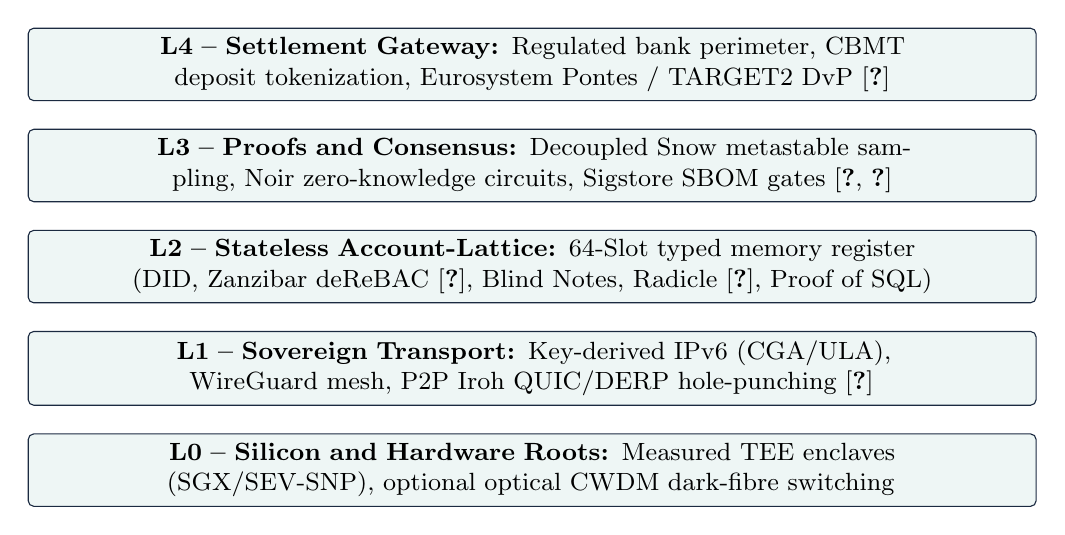
\begin{tikzpicture}[
  layer/.style={draw=ink,rounded corners=2pt,minimum width=12.8cm,text width=12.2cm,minimum height=9mm,
                align=center,fill=accent!7,font=\small},
  node distance=3.5mm]
  \node[layer] (l0) {\textbf{L0 -- Silicon and Hardware Roots:} Measured TEE enclaves (SGX/SEV-SNP), optional optical CWDM dark-fibre switching};
  \node[layer,above=of l0] (l1) {\textbf{L1 -- Sovereign Transport:} Key-derived IPv6 (CGA/ULA), WireGuard mesh, P2P Iroh QUIC/DERP hole-punching~\cite{iroh2024}};
  \node[layer,above=of l1] (l2) {\textbf{L2 -- Stateless Account-Lattice:} 64-Slot typed memory register (DID, Zanzibar deReBAC~\cite{pang2019zanzibar}, Blind Notes, Radicle~\cite{radicle2024}, Proof of SQL)};
  \node[layer,above=of l2] (l3) {\textbf{L3 -- Proofs and Consensus:} Decoupled Snow metastable sampling, Noir zero-knowledge circuits, Sigstore SBOM gates~\cite{newman2022sigstore,torresarias2019intoto}};
  \node[layer,above=of l3] (l4) {\textbf{L4 -- Settlement Gateway:} Regulated bank perimeter, CBMT deposit tokenization, Eurosystem Pontes / TARGET2 DvP~\cite{ecbpontes}};
\end{tikzpicture}
\caption{The Sovereign Stack 5-layer hierarchy. Each layer is cleanly decoupled; trust invariants strengthen toward Layer~4.}
\label{fig:stack}
\end{figure}

\subsection{State: The Stateless Account-Lattice}

Traditional blockchain architectures (e.g., Ethereum, Solana) enforce a single global
mutable state trie, requiring every validator to process and sequence every transaction
globally. This creates artificial state congestion, forcing users into auction-based gas
bidding wars.

The Sovereign Stack adopts an actor-based \textbf{stateless account-lattice} model. Every account,
smart contract, and zero-knowledge circuit operates as an autonomous \textbf{Actor} governing
its own independent, append-only micro-chain of state transitions. Account owners and smart contracts
execute state transitions unilaterally by providing valid monotonic sequence nonces and
cryptographic signatures. Crucially, inter-account coordination does not require public state contention:
actors communicate and coordinate via \textbf{native Blind Notes} (Aztec-style private notes~\cite{williamson2022aztec} carrying Pedersen commitments~\cite{pedersen1991commitment},
commitments, Poseidon nullifiers, and viewing keys).

Network validators do not store full historical ledger states; they verify succinct zero-knowledge
transition proofs (authored in Noir~\cite{aztec2021noir} and verified as UltraPlonk SNARKs~\cite{gabizon2019plonk}), process sub-10ms transaction batches via Rotating Paxos~\cite{lamport1998paxos,lamport2001paxos}, and update constant-sized Merkle
roots across epochs via Decoupled Snow.

\subsection{zkOIDC: Zero-Knowledge OpenID Connect and Enterprise Web 2.5 Identity}
\label{sec:zkoidc}

A primary friction point in onboarding enterprise workforces and community members into sovereign cryptographic environments is identity initialization: requiring users to immediately master hardware seed phrases, cold signers, or complex air-gapped key management creates severe organizational friction. Conversely, relying on standard Web2 federated identity (OAuth2 / OpenID Connect~\cite{oidc2014}) exposes users to pervasive tracking, corporate surveillance, and centralized de-platforming risks.

Pioneering identity infrastructure developed by Spruce Systems established the modern bridge between Web2 authentication and cryptographic accounts via \textbf{Sign-In with Ethereum (EIP-4361)}~\cite{spruceid2022siwe} and W3C Verifiable Credentials through DIDKit~\cite{dif2021did}. By allowing users to sign structured messages proving control of on-chain accounts to traditional web servers, SpruceID demonstrated that decentralized identity could integrate cleanly with existing institutional workflows without sacrificing user ownership.

The Sovereign Bunny architecture takes this foundational bridge and elevates it to client-side zero knowledge via \textbf{zkOIDC (Zero-Knowledge OpenID Connect)}:
\begin{enumerate}
  \item \textbf{Web2 Identity Assertion:} The user logs into an existing institutional identity provider (e.g., Google Workspace, GitHub, Microsoft Azure AD, or enterprise Okta) through standard browser flows, receiving an authentic JSON Web Token (JWT) signed by the provider's RSA-2048, RSA-4096, or ECDSA private key.
  \item \textbf{Client-Side Zero-Knowledge JWT Proof ($\pi_{\text{OIDC}}$):} Rather than exposing the plaintext JWT or user metadata on-chain, the client's Sovereign Wallet or in-browser WASM worker executes a specialized Noir / UltraPlonk zero-knowledge circuit~\cite{aztec2021noir,gabizon2019plonk}:
  \begin{itemize}
    \item Verifies the RSA/ECDSA digital signature against the identity provider's publicly committed JSON Web Key Set (JWKS) root committed in CAR Slot~0 ($R_0$).
    \item Verifies token validity timestamps ($\text{iat} \le \text{now} \le \text{exp}$), proving non-expiration without revealing the exact issuance epoch.
    \item Evaluates organizational and domain predicate constraints (such as asserting that the claimant's email belongs to an authorized enterprise domain \code{@company.com} or fulfills a verified KYC tier) \textbf{without disclosing the user's email address, legal name, or personal identity}.
    \item Computes an un-linkable, deterministic identity nullifier:
    \begin{equation}
      \text{Null}_{\text{OIDC}} = \text{Poseidon}(\text{salt}, \text{sub}, \text{aud})
    \end{equation}
  \end{itemize}
  \item \textbf{Slot~0 DID Integration:} The resulting succinct proof $\pi_{\text{OIDC}}$ binds the Web2 assertion directly to the user's sovereign W3C DID in Slot~0 ($R_0$)~\cite{w3cdid2022}.
  \item \textbf{Fail-Closed Security:} This completely resolves the Web sign-in verifier regression (\cref{tab:status}): eliminating mock signature bypasses, enforcing strict cryptographic expiration, and ensuring that any forged or revoked JWT fails closed instantly.
\end{enumerate}

\subsection{The Lattice Saga Protocol: Synchronous Compatibility and Configurable Account Locking}
\label{sec:saga_locking}

Because the Sovereign Bunny architecture operates as a stateless account-lattice where each account is an independent, single-writer micro-chain~\cite{lemahieu2018nano,buterin2021stateless}, transactions achieve extreme concurrency without global state trie contention. However, legacy EVM protocols and composite financial contracts (such as re-entrant flash loans, atomic cross-contract liquidity sweeps, and multi-party escrow) implicitly rely on synchronous global state locks.

To reconcile single-writer micro-chains with legacy synchronous expectations without introducing global locking bottlenecks, the runtime implements the \textbf{Lattice Saga Protocol}:
\begin{enumerate}
  \item \textbf{Saga Reservation Intent:} An initiator actor emits an atomic intent referencing $N$ participant accounts, providing cryptographic commitments to the expected input and output states in Slot~2.
  \item \textbf{Configurable Saga Account Locking:} Participating accounts can enter a temporary \textbf{Saga Lock} ($\text{Lock}_{\text{saga}} = \text{true}$ in Slot~5):
  \begin{itemize}
    \item While locked, the account's single-writer sequencer rejects conflicting out-of-band balance mutations.
    \item The lock is strictly bounded by an epoch timeout parameter $E_{\text{timeout}}$ (default: 3 epochs, $\sim 15$ seconds).
    \item If the multi-account saga completes, an aggregate transition proof is committed, and all locks are released atomically.
    \item If any participant fails or times out, a deterministic compensating transaction (rollback proof) is executed, releasing locked escrow funds without leaving dangling states.
  \end{itemize}
  \item \textbf{Canonical Lexicographical Lock Acquisition Invariant:} To mathematically prevent distributed deadlock conditions (classic $A \to B \to C \to A$ circular wait-dependencies across concurrent sagas), participant accounts MUST be locked in strict ascending lexicographical order of their canonical W3C DIDs:
  \begin{equation}
    \text{Lock}(u_i) \prec \text{Lock}(u_j) \iff \operatorname{DID}(u_i) <_{\text{lex}} \operatorname{DID}(u_j)
  \end{equation}
  By Dijkstra's resource hierarchy theorem and the Chandy-Misra-Haas condition, enforcing a strict total order over lock acquisition guarantees that cyclic wait-for dependency graphs cannot form. Furthermore, the runtime implements \textbf{Fail-Fast Lock Contention}: if a required account along the sorted sequence is already locked by a concurrent saga, the lock attempt fails closed instantly rather than stalling for the 15-second $E_{\text{timeout}}$ window, triggering immediate compensating rollbacks and preserving sub-second clearing velocity.
  \item \textbf{Explicit Opt-Out Configuration Invariant:} Crucially, saga locking is fully configurable per account. Autonomous edge daemons, IoT nodes, and high-frequency market makers configure $\code{allow\_saga\_locking} = \code{false}$ in their Slot~5 policy byte. This guarantees that external contracts cannot lock or freeze their local micro-chain under any circumstances; interactions with opt-out accounts must proceed asynchronously via native Blind Notes and Pedersen commitments~\cite{pedersen1991commitment}.
\end{enumerate}

\subsection{The 64-Slot Typed Account Register}

Every sovereign account maintains a 64-slot typed memory register (\cref{fig:register_layout}).
Each slot represents an isolated cryptographic commitment governed by specialized
execution rules and precompile contracts (\cref{tab:slots_spec}).

\begin{figure}[H]
\centering
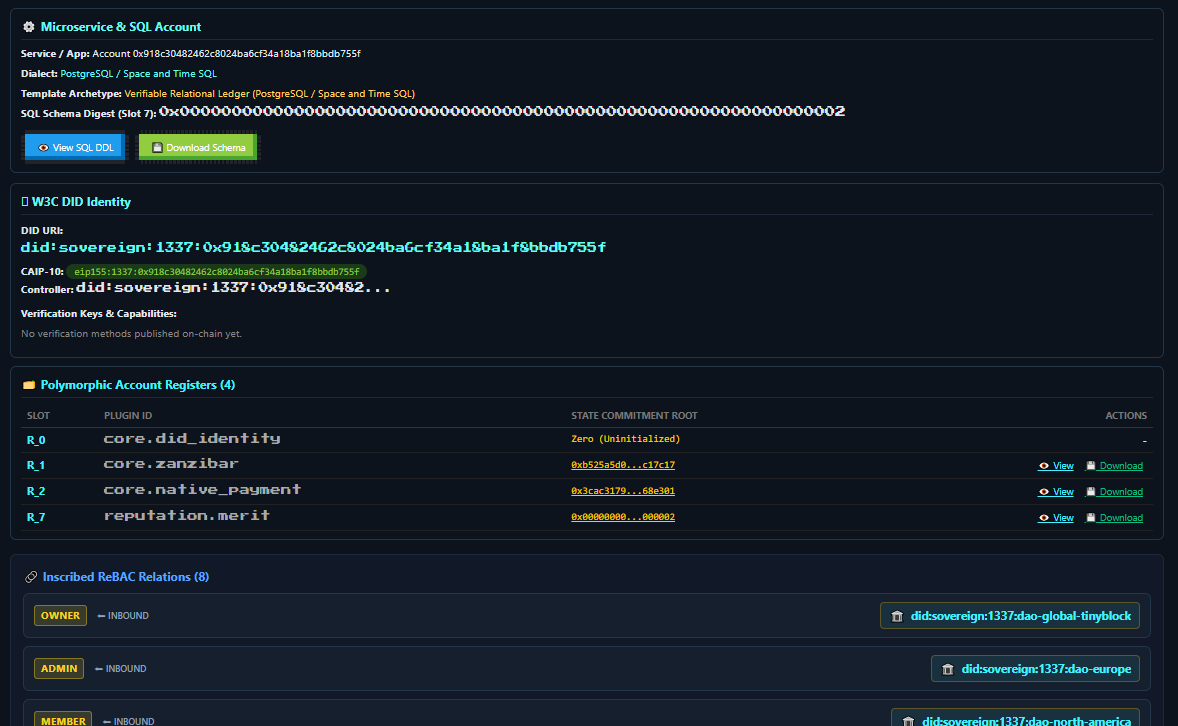
\includegraphics[width=0.88\linewidth]{img/sovereign_wallet_slots.png}
\caption{Cryptographic memory layout of an account register on the stateless lattice, showing typed Slot~0 through Slot~63 allocations.}
\label{fig:register_layout}
\end{figure}

\begin{figure}[H]
\centering
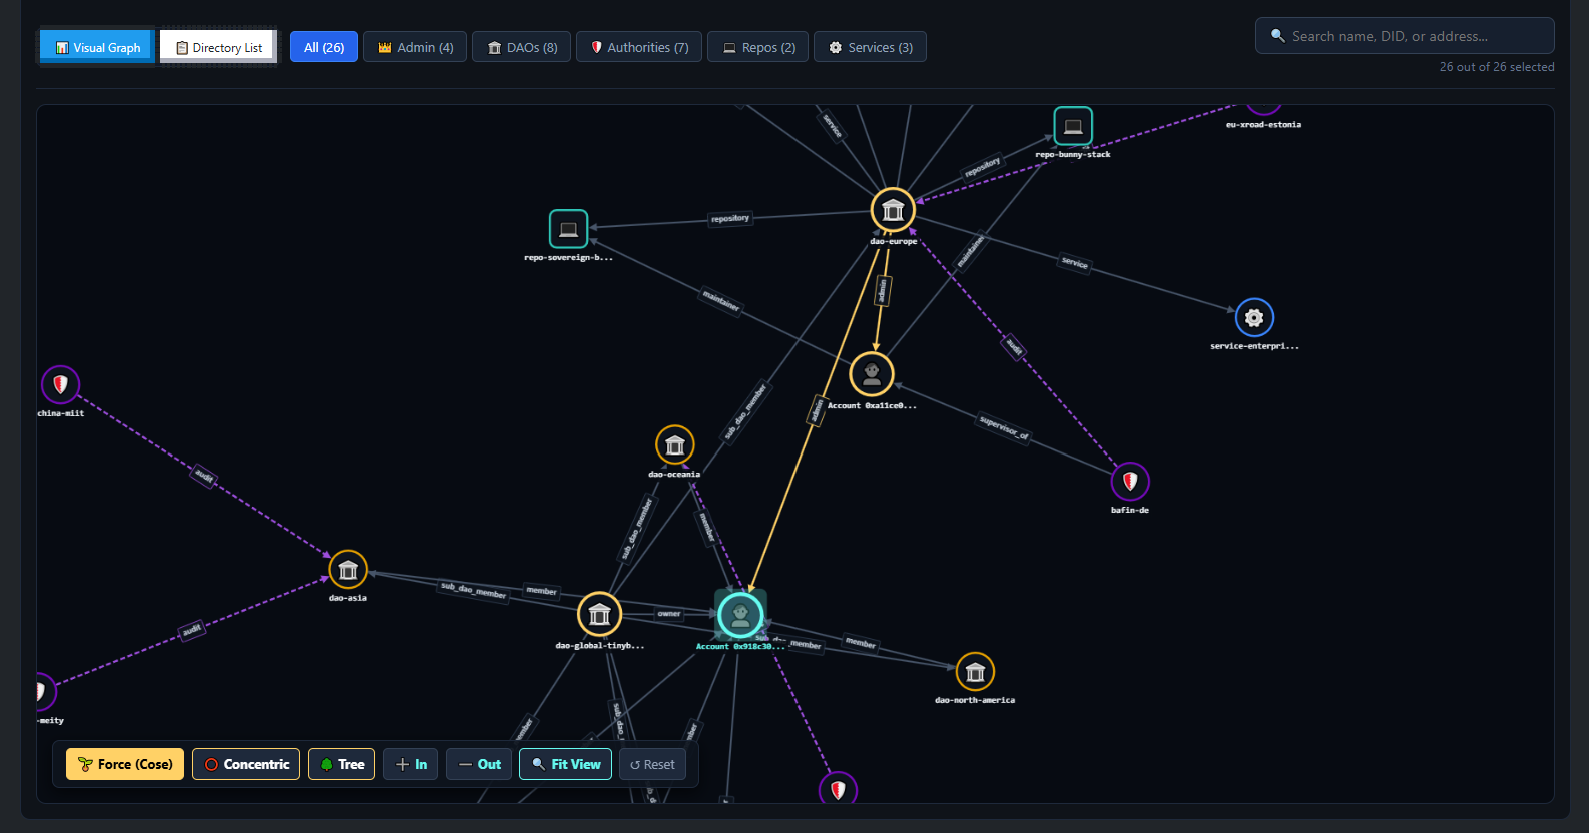
\includegraphics[width=0.88\linewidth]{img/deReBAC_Explorer.png}
\caption{Decentralized Relationship-Based Access Control (deReBAC) graph explorer resolving Google Zanzibar tuples in Slot~1~\cite{pang2019zanzibar}.}
\label{fig:derebac_explorer}
\end{figure}

\begin{table}[htbp]
\centering\scriptsize
\renewcommand{\arraystretch}{1.25}
\begin{tabularx}{\linewidth}{@{}l L{2.6cm} L{2.2cm} L{1.8cm} Y@{}}
\toprule
\textbf{Slot} & \textbf{Subsystem \& Identifier} & \textbf{Data Structure} & \textbf{Storage Policy} & \textbf{Cryptographic Invariant \& Function}\\
\midrule
Slot~0 ($R_0$) & W3C / DIF DID Identity~\cite{w3cdid2022,dif2021did} & BLAKE3 Document CID & Cold Pinned & Identity root, QSCD keys, zkvIBAN, and dynamic risk-adjusted KYC credentials\\
Slot~1 ($R_1$) & Zanzibar deReBAC~\cite{pang2019zanzibar} & SMT Merkle Root & Cold Pinned & Relation tuples (\code{user\#relation@object}) governing role-based authorization\\
Slot~2 ($R_2$) & Blind Note Register~\cite{williamson2022aztec,pedersen1991commitment} & CAR BLAKE3 Root & Dynamic CAR & Private bearer notes, viewing keys, homomorphic Pedersen commitments\\
Slot~3 ($R_3$) & Radicle Git Repository & SMT / Radicle DAG & Dynamic CAR & Git reference tree, commit SHA, MuSig2 threshold signatures, SBOM root\\
Slot~4 ($R_4$) & Proof of SQL Table State & IPA / Merkle Root & Dynamic CAR & Relational database commitments (NextERP / PostgreSQL state accumulator)\\
Slot~5 ($R_5$) & Epoch Engine Consensus & Epoch Transition SMT & Dynamic CAR & Rotating Paxos lease, Fediverse / ActivityPub state, epoch transition proofs\\
Slot~6 ($R_6$) & Regional DAO Governance & Ballot SMT Matrix & Dynamic CAR & Federated regional DAO voting ballots, non-self-dealing quorum matrices\\
Slot~7 ($R_7$) & Lattice Saga Lock \& Policy & Bitmask \& Lock Queue & Dynamic CAR & Single-writer writer-lease, \code{allow\_saga\_locking} policy byte, cross-actor lock state\\
Slot~8 ($R_8$) & Operational Surety Bonds & Bonded Token SMT & Dynamic CAR & Operational surety escrows (locked \$RAD / \$TINY), canonical routing bonds, equivocation slashing collateral\\
Slots~9--63 & Dynamic Sparse Slots & Deterministic Hash & On-Demand & Bounded allocation via \code{derive\_slot\_id(name)}: BGP tokens, IoT telemetry, FHE state\\
\bottomrule
\end{tabularx}
\caption{Full specification of the 64-Slot Microkernel Account Register (CAR) on the Sovereign Bunny Account-Lattice.}
\label{tab:slots_spec}
\end{table}

\subsubsection{Noir Cross-Slot Verification Circuit: Asserting Git, Zanzibar, and SQL Roots}

A pivotal capability of the 64-slot architecture is \textbf{cross-slot zero-knowledge verification}:
asserting relationships across disparate slots without leaking identity or intermediate data.
In the circuit below (\cref{lst:cross_slot_noir}), the verifier asserts that a software release
binary committed to Slot~3 was published by a developer with the \code{maintainer} role in
Slot~1, ratified by $\ge k$ regional DAOs in Slot~6, and logged into the Slot~4 database audit accumulator:

\Needspace{25\baselineskip}
\begin{lstlisting}[language=Noir,label=lst:cross_slot_noir,caption={Noir Circuit: Cross-Slot Verification of Git Build Provenance, Zanzibar ReBAC, and Proof of SQL (\code{circuits/src/cross\_slot\_verifier.nr})}]
use dep::std::merkle::compute_merkle_root;

// CAR Slot Cross-Verification Circuit: Proves that a Git release binary (Slot 3)
// is authorized by a verified maintainer DID (Slot 0 & Slot 1) and ratified
// by a regional DAO quorum (Slot 6), with audit trace committed to Proof of SQL (Slot 4).
fn main(
    // Public Inputs (Canonical CAR slot roots on account lattice)
    slot_0_did_root: pub Field,
    slot_1_zanzibar_root: pub Field,
    slot_3_git_root: pub Field,
    slot_4_sql_root: pub Field,
    slot_6_dao_matrix_root: pub Field,

    // Private Witness Inputs
    developer_did: Field,
    did_merkle_path: [Field; 16],
    did_index: Field,

    // Slot 1: Zanzibar ReBAC Proof (proves developer has 'maintainer' on repository)
    relation_tuple_hash: Field,
    zanzibar_merkle_path: [Field; 16],
    zanzibar_index: Field,

    // Slot 3: Git provenance (commit tree hash of the reproducible build)
    git_commit_hash: Field,
    git_merkle_path: [Field; 16],
    git_index: Field,

    // Slot 6: Regional DAO Multi-Federation Ratification
    dao_ballot_hash: Field,
    dao_matrix_merkle_path: [Field; 16],
    dao_index: Field,
    dao_approval_bitmap: Field, // Asserts >= k regions ratified release

    // Slot 4: Proof of SQL audit row (release log entry)
    sql_audit_row_hash: Field,
    sql_merkle_path: [Field; 16],
    sql_index: Field
) {
    // 1. Verify Developer DID is committed in Slot 0 Root
    let computed_did_root = compute_merkle_root(developer_did, did_index, did_merkle_path);
    assert(computed_did_root == slot_0_did_root);

    // 2. Verify Maintainer ReBAC Relation in Slot 1
    let computed_zanzibar_root = compute_merkle_root(relation_tuple_hash, zanzibar_index, zanzibar_merkle_path);
    assert(computed_zanzibar_root == slot_1_zanzibar_root);

    // 3. Verify Git Release Binary Commit is in Slot 3
    let computed_git_root = compute_merkle_root(git_commit_hash, git_index, git_merkle_path);
    assert(computed_git_root == slot_3_git_root);

    // 4. Verify Regional DAO Federation Ratification in Slot 6
    let computed_dao_root = compute_merkle_root(dao_ballot_hash, dao_index, dao_matrix_merkle_path);
    assert(computed_dao_root == slot_6_dao_matrix_root);
    assert(dao_approval_bitmap != 0);

    // 5. Verify Proof of SQL Audit Log Committed in Slot 4
    let computed_sql_root = compute_merkle_root(sql_audit_row_hash, sql_index, sql_merkle_path);
    assert(computed_sql_root == slot_4_sql_root);
}
\end{lstlisting}

\subsection{Confidential Coordination: Privacy-Preserving Proposal Voting via Native Blind Notes}
\label{sec:confidential_voting}

A catastrophic pathology of legacy DAO governance systems is public ballot exposure: token-weighted
votes are broadcast openly to public mempools, exposing participants to coercion, vote-buying,
whistleblower retaliation, and economic front-running.

In the Sovereign Bunny block-lattice, \textbf{every smart contract and Noir verification circuit is an autonomous Actor}
possessing its own single-writer micro-chain, 64-slot CAR register, and strongly typed interface.
Inter-actor governance and proposal coordination operate through \textbf{native Blind Notes} ($R_2$)
rather than shared mutable state:
\begin{enumerate}
  \item \textbf{Private Voting Note Minting:} A governance participant holds an unspent Blind Note in Slot~2
representing their non-transferable voting weight, derived from verified TinyMeritRank or enterprise seat licenses.
The note encapsulates the voter's power behind a Pedersen commitment $C = \text{Commit}(\text{Weight},\, r)$.
  \item \textbf{Confidential Ballot Dispatch:} To vote on a proposal, the participant dispatches an encrypted note
into the DAO Actor's note inbox. The note payload hides the proposal identifier and vote choice:
  \begin{equation}
    C_{\text{ballot}} = \text{Commit}(\text{ProposalID} \parallel \text{VoteChoice} \parallel \text{Weight},\, r_{\text{ballot}})
  \end{equation}
  \item \textbf{Zero-Knowledge Capability \& Ballot Verification:} The voter submits a succinct Noir proof asserting:
  \begin{itemize}
    \item \textbf{Zanzibar deReBAC Authorization ($R_1$):} The voter's DID possesses the required role (e.g. \code{dao:region\_eu\#member@user\_did}) in the DAO's on-chain relationship graph.
    \item \textbf{Note Membership ($R_2$):} The voting note exists in the canonical Blind Note Merkle tree.
    \item \textbf{Nullifier Uniqueness ($R_2$):} The nullifier $\text{Nullifier} = \mathcal{H}(\text{NoteID},\, \text{SecretKey})$ is uniquely derived and not previously spent, preventing double-voting.
  \end{itemize}
  \item \textbf{Tallying Without Identity Exposure:} The DAO Actor tallies encrypted ballots homomorphically or via
succinct zero-knowledge batch circuits. Quorum thresholds and outcomes are proven mathematically while
individual voter identities, specific voting weights, and choices remain completely private.
\end{enumerate}

\subsubsection{Hierarchical Private Coordination: Scaling Voting via Nested Sub-DAO Accumulators}
\label{sec:hierarchical_dao_voting}

Direct global on-chain balloting inevitably collapses into one of two systemic failures: either public vote exposure
destroys privacy and enables coercion, or massive monolithic tally circuits become computationally intractable
for global populations.

The Sovereign Bunny architecture resolves this bottleneck by formalizing governance as a \textbf{tree of nested sub-DAOs}
reflecting Elinor Ostrom's Principle~8 (Nested Enterprises) and human sociological Dunbar groupings:
\begin{enumerate}
  \item \textbf{Local Working Circles (Sub-Sub-Sub DAOs):} At the localized base layer (e.g. a specific municipal fiber-splicing team, software maintenance working group, or regional hackerspace circle of 15--150 participants), members submit encrypted Blind Notes ($R_2$) into a local leaf accumulator.
  \item \textbf{Intermediate Zero-Knowledge Rollup Aggregation:} The sub-sub DAO operator or elected delegate does not publish individual ballots. Instead, they execute a succinct Noir aggregation circuit asserting:
  \begin{itemize}
    \item Every included note satisfies local Zanzibar deReBAC membership ($R_1$).
    \item Every nullifier is uniquely spent and added to the local nullifier SMT ($R_2$).
    \item The encrypted vector sum of affirmative and negative tallies matches the committed accumulator root.
  \end{itemize}
  The sub-sub DAO emits a single succinct recursive proof ($\pi_{\text{sub}}$) and a aggregated tally commitment.
  \item \textbf{Federated Regional Assembly (Sub-DAO):} Regional DAOs ingest the verified tally commitments of their constituent working circles, aggregating them into a regional accumulator proof ($\pi_{\text{regional}}$).
  \item \textbf{Global Manifold Finality:} The global Sovereign Bunny ledger verifies the regional proofs in $O(1)$ time ($< 5$\,ms). Governance scales arbitrarily to millions of participants without monolithic state bottlenecks, while individual voter identities and specific voting weights remain mathematically hidden within their local sub-DAO leaf accumulators.
\end{enumerate}

\subsection{Radicle Git Slots: Verifiable Code Release and Raw Git Compatibility}
\label{sec:radicle_slots}

Slot~3 elevates a Radicle Git repository to a first-class state primitive on the
distributed ledger. Canonical repository tips (\code{refs/heads/*}, \code{refs/tags/*})
advance strictly through executed precompile transactions satisfying:
(1)~monotonic slot nonces,
(2)~authorized W3C DID signatures,
(3)~$k$-of-$n$ delegate MuSig2 threshold aggregation, and
(4)~deReBAC capability checks.

The precompile enforces $O(1)$ scalar root updates without unpacking raw packfiles
on-chain. Furthermore, supply-chain invariants are baked directly into the promotion
logic: every release tag (\code{refs/tags/v*}) must supply a zero-knowledge SNARK proof
asserting that the Git tree contains a valid CycloneDX Software Bill of Materials (SBOM)
satisfying SLSA Level~3 and non-membership against a banned Common Vulnerabilities and
Exposures (CVE) Merkle tree.

\subsubsection{Rust Reference Precompile: Radicle Slot 3 Canonical Promotion}

The following production Rust precompile implementation enforces state promotion,
monotonic nonces, and zero-knowledge SBOM compliance:

\Needspace{25\baselineskip}
\begin{lstlisting}[language=Rust,caption={Rust Precompile: Radicle Slot 3 Canonical Promotion and SBOM Compliance Gate (\code{contracts/precompiles/src/radicle\_slot.rs})}]
use sha2::{Digest, Sha256};

pub const RADICLE_SLOT_INDEX: u8 = 3;

#[derive(Clone, Debug, PartialEq, Eq)]
pub struct RadicleSlotState {
    pub nonce: u64,
    pub ref_root: [u8; 32],      // Sparse Merkle Root of canonical refs
    pub id_hash: [u8; 32],       // BLAKE3 hash of canonical rad/id doc
    pub derebac_root: [u8; 32],  // Root of relationship access graph
    pub sbom_digest: [u8; 32],   // ZK predicate digest: SLSA L3 & zero banned CVEs
}

pub struct TransitionIntent {
    pub target_ref: String,
    pub new_commit_sha: [u8; 20],
    pub proposed_nonce: u64,
    pub zk_sbom_proof: Vec<u8>,
    pub aggregate_sig: Vec<u8>,
}

impl RadicleSlotState {
    pub fn verify_and_apply(
        &mut self,
        intent: TransitionIntent,
        banned_cve_root: [u8; 32],
    ) -> Result<(), &'static str> {
        // 1. Monotonic Nonce Check (Strict Anti-Replay Protection)
        if intent.proposed_nonce <= self.nonce {
            return Err("REVERT: Nonce must strictly increment monotonically");
        }

        // 2. Validate Multi-Signature Aggregate over Canonical State Update
        let mut hasher = Sha256::new();
        hasher.update(&self.ref_root);
        hasher.update(&intent.new_commit_sha);
        hasher.update(&intent.proposed_nonce.to_le_bytes());
        let digest = hasher.finalize();

        if !verify_musig2_threshold(&self.id_hash, &digest, &intent.aggregate_sig) {
            return Err("REVERT: Invalid delegate signature threshold");
        }

        // 3. Verify CRA/NIS2 Zero-Knowledge SBOM Compliance Circuit
        // Proof asserts: Git Tree contains valid CycloneDX SBOM matching commit_sha
        // AND non-membership proof against banned_cve_root.
        let sbom_valid = verify_zk_snark_sbom(
            &intent.zk_sbom_proof,
            &intent.new_commit_sha,
            &banned_cve_root,
        );
        if !sbom_valid {
            return Err("REVERT: Supply-chain verification failed CRA compliance check");
        }

        // 4. Update Slot State Digest (O(1) Constant Memory Footprint)
        self.nonce = intent.proposed_nonce;
        self.ref_root = update_smt_ref(&self.ref_root, &intent.target_ref, &intent.new_commit_sha);
        self.sbom_digest = Sha256::digest(&intent.zk_sbom_proof).into();

        Ok(())
    }
}
\end{lstlisting}

\subsection{Proof of SQL Verifier for ERP Systems (Slot 4)}

Enterprise resource planning systems (ERPNext, PostgreSQL, MariaDB) maintain sensitive
relational tables. To enable external auditing without compromising proprietary line items,
Slot~4 stores cryptographic polynomial commitments over table column vectors.
Auditors verify zero-knowledge Inner-Product Arguments (IPA) asserting inventory or
accounting balance invariants:

\Needspace{25\baselineskip}
\begin{lstlisting}[language=Rust,caption={Rust Precompile: Proof of SQL Verifier for ERPNext / PostgreSQL (\code{contracts/precompiles/src/proof\_of\_sql.rs})}]
pub const SQL_SLOT_INDEX: u8 = 4;

pub struct SqlTableCommitment {
    pub table_id: [u8; 16],
    pub row_count: u64,
    pub polynomial_commitment: [u8; 32], // KZG or IPA commitment over column vectors
}

pub struct SqlAuditProof {
    pub query_hash: [u8; 32],            // e.g., H("SELECT SUM(amount) FROM invoices WHERE paid=true")
    pub expected_result: u128,
    pub proof_bytes: Vec<u8>,
}

pub fn verify_sql_audit_query(
    commitment: &SqlTableCommitment,
    proof: &SqlAuditProof,
) -> bool {
    // Verifies an Inner-Product Argument over the committed table polynomial.
    // The prover proves that P(x) evaluated over the filtered selector columns
    // equals the expected aggregate sum without revealing individual rows or customer metadata.
    ipa_verify(
        &commitment.polynomial_commitment,
        proof.query_hash,
        proof.expected_result,
        &proof.proof_bytes,
    )
}
\end{lstlisting}

\subsubsection{Rust Implementation: Proof of SQL Table Schema and Row Commitment Engine}
\label{sec:sql_anchor_code}

To anchor relational database tables (ERPNext, PostgreSQL) into Slot~4 without disclosing confidential
customer rows, the host engine compiles table schemas and data rows into polynomial column commitments
and Merkle tree roots committed to the account register:

\Needspace{25\baselineskip}
\begin{lstlisting}[language=Rust,caption={Rust Implementation: Proof of SQL Schema and Row Commitment Engine (\code{crates/db/src/sql\_row\_anchor.rs})}]
use sha2::{Digest, Sha256};

pub struct SqlColumnSchema {
    pub column_name: String,
    pub data_type: u8, // 1: Integer, 2: FixedDecimal, 3: Utf8Digest
    pub is_indexed: bool,
}

pub struct SqlTableStateAnchor {
    pub schema_digest: [u8; 32],
    pub row_count: u64,
    pub column_roots: Vec<[u8; 32]>,   // Polynomial column vector commitments
    pub table_merkle_root: [u8; 32],   // Root committed to CAR Slot 4
}

impl SqlTableStateAnchor {
    pub fn commit_invoice_row(
        &mut self,
        invoice_id: u64,
        debtor_did: [u8; 32],
        creditor_did: [u8; 32],
        amount_eure: u128,
        rwa_collateral_flag: bool,
        salt: [u8; 32],
    ) -> [u8; 32] {
        // 1. Serialize row into canonical typed vector
        let mut hasher = Sha256::new();
        hasher.update(&self.schema_digest);
        hasher.update(&invoice_id.to_le_bytes());
        hasher.update(&debtor_did);
        hasher.update(&creditor_did);
        hasher.update(&amount_eure.to_le_bytes());
        hasher.update(&[rwa_collateral_flag as u8]);
        hasher.update(&salt);
        let row_commitment: [u8; 32] = hasher.finalize().into();

        // 2. Insert into incremental Merkle tree and advance row counter
        self.row_count += 1;
        self.table_merkle_root = self.compute_updated_root(row_commitment);
        row_commitment
    }

    fn compute_updated_root(&self, row_hash: [u8; 32]) -> [u8; 32] {
        let mut h = Sha256::new();
        h.update(&self.table_merkle_root);
        h.update(&row_hash);
        h.finalize().into()
    }
}
\end{lstlisting}

\subsection{Dynamic SLA Escrow Contract}
\label{sec:dsla_escrow}

To enforce operational accountability between enterprise clients and sovereign edge
host operators, payments flow through a dynamic SLA escrow smart contract. Performance
oracles evaluate node uptime and latency; any breach triggers automated contractual slashing:

\Needspace{25\baselineskip}
\begin{lstlisting}[language=Solidity,caption={Solidity Smart Contract: Dynamic SLA Escrow with Oracle-Enforced Slashing (\code{contracts/src/DSLAServiceEscrow.sol})}]
// SPDX-License-Identifier: Apache-2.0
pragma solidity ^0.8.24;

interface IHeartbeatOracle {
    function getUptimeMetrics(address provider) external view returns (uint256 uptimeBps, uint256 latencyMs);
}

contract DSLAServiceEscrow {
    struct SLA {
        address client;
        address provider;
        uint256 deposit;
        uint256 ratePerBlock;
        uint256 lastSettledBlock;
        uint256 maxLatencyMs;
        uint256 minUptimeBps;
    }

    mapping(uint256 => SLA) public slas;
    IHeartbeatOracle public immutable oracle;

    event Slashed(uint256 indexed slaId, uint256 penaltyAmount);
    event Settled(uint256 indexed slaId, uint256 payoutAmount);

    constructor(address _oracle) {
        oracle = IHeartbeatOracle(_oracle);
    }

    function settleSLA(uint256 slaId) external {
        SLA storage sla = slas[slaId];
        require(block.number > sla.lastSettledBlock, "Already settled");

        uint256 blocks = block.number - sla.lastSettledBlock;
        uint256 owed = blocks * sla.ratePerBlock;

        (uint256 uptimeBps, uint256 latencyMs) = oracle.getUptimeMetrics(sla.provider);

        // Automated DSLA Performance Check
        if (uptimeBps < sla.minUptimeBps || latencyMs > sla.maxLatencyMs) {
            uint256 penalty = owed; // 100% penalty for SLA breach during interval
            sla.deposit -= penalty;
            payable(sla.client).transfer(penalty);
            emit Slashed(slaId, penalty);
        } else {
            sla.deposit -= owed;
            payable(sla.provider).transfer(owed);
            emit Settled(slaId, owed);
        }

        sla.lastSettledBlock = block.number;
    }
}
\end{lstlisting}

\subsection{The Ledger as Orchestration API: In-Browser Sovereign SSH}
\label{sec:sovereign_ssh}

Rather than relying on Amazon AWS IAM, proprietary hypervisor management platforms, or
centralized SaaS dashboards, the Sovereign Account-Lattice functions as the
bare-metal deployment and orchestration API:

\begin{figure}[htbp]
\centering
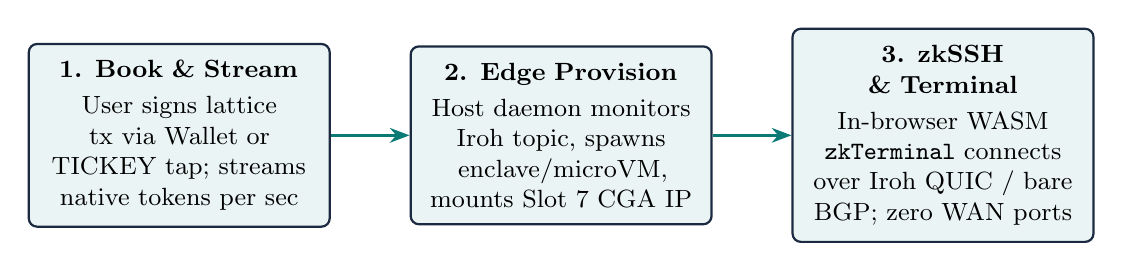
\begin{tikzpicture}[
  node distance=1.0cm,
  block/.style={draw=ink, fill=accent!8, rounded corners=3pt, line width=0.8pt, font=\small, inner sep=6pt, text width=3.4cm, align=center},
  arrow/.style={-{Stealth[length=2.5mm]}, line width=1pt, draw=accent}
]
  \node[block] (book) {\textbf{1. Book \& Stream}\\[2pt]User signs lattice tx via Wallet or TICKEY tap; streams native tokens per sec};
  \node[block, right=1.0cm of book] (prov) {\textbf{2. Edge Provision}\\[2pt]Host daemon monitors Iroh topic, spawns enclave/microVM, mounts Slot~7 CGA IP};
  \node[block, right=1.0cm of prov] (access) {\textbf{3. zkSSH \& Terminal}\\[2pt]In-browser WASM \code{zkTerminal} connects over Iroh QUIC / bare BGP; zero WAN ports};

  \draw[arrow] (book) -- (prov);
  \draw[arrow] (prov) -- (access);
\end{tikzpicture}
\caption{The ``Book, Boot \& Shell'' Workflow: Automated bare-metal provisioning, direct cryptographic addressing, and in-browser zkSSH terminal sessions over P2P Iroh QUIC and BGP transports.}
\label{fig:ssh_workflow}
\end{figure}

The \textbf{``Book, Boot \& Shell''} workflow operates in three frictionless steps:
\begin{enumerate}
  \item \textbf{Lattice Booking Intent:} The user executes an on-chain lease transaction
via their Sovereign Wallet or TICKEY badge tap. The payload specifies hardware
specifications, cluster geographic preferences, lease duration, and the tenant's
Ed25519 SSH public key.
  \item \textbf{Encrypted Iroh Blob Dispatch:} The commitment is serialized into an encrypted
Iroh blob referenced by a BLAKE3 root in Slot~2.
  \item \textbf{Automated Bare-Metal Provisioning:} An autonomous host daemon running on an
edge micro-server or colocation blade monitors the Iroh topic:
\begin{itemize}
\item Validates the cryptographic payment receipt and SLA ticket state.
\item Spawns an isolated microVM or container jail pre-configured with the tenant's
private Radicle network keys.
\item Appends the tenant's Ed25519 public key to the container's \code{authorized\_keys}.
\end{itemize}
  \item \textbf{Zero-Trust In-Browser Sovereign SSH:} The browser loads an \code{xterm.js}
terminal powered by a WebAssembly-compiled SSH client. When the user initiates
connection, the client signs an ephemeral session challenge using the private key
held in their hardware token or TICKEY badge. Traffic routes directly through Iroh's
peer-to-peer transport over QUIC with DERP hole-punching. The entire connection
requires \textbf{zero public IPv4 addresses, zero open firewall ports, zero VPN
concentrators, and zero central bastion servers}.
\end{enumerate}

\subsection{Autonomous AI Agents: Budget Wallets, zkSSH vServer Booking, and Deterministic Reboots}
\label{sec:ai_agent_zkssh}

The convergence of autonomous artificial intelligence agents and decentralized ledgers has historically been crippled
by binary extremes: either giving an untrusted agent unconstrained private key access (risking total treasury drain),
or requiring human manual approval for every operational API call (destroying agentic autonomy).

In the Sovereign Bunny stack, an enterprise client or human developer who has already completed dynamic risk-adjusted
KYC in Slot~0 can delegate a strictly bounded operational wallet to an \textbf{autonomous AI agent keypair}:
\begin{enumerate}
  \item \textbf{Zanzibar deReBAC Delegation ($R_1$):} The human principal registers an on-chain authorization tuple:
  \begin{equation}
    \text{\ttfamily cluster:eu\_fleet\#provisioner@agent\_did} \quad \text{with} \quad \text{\ttfamily max\_budget: 500\_EURe}
  \end{equation}
  \item \textbf{Autonomous vServer Booking via Dynamic Escrow:} The AI agent detects a computational requirement, queries bare-metal node providers over BGP, and autonomously executes a lease transaction against \code{DSLAServiceEscrow.sol} (\cref{sec:dsla_escrow}), depositing up to its pre-allocated budget.
  \item \textbf{In-Browser zkSSH Access:} The agent establishes a direct \textbf{zkSSH} connection over Iroh QUIC to the provisioned microVM, authenticating via its delegated DID signature without disclosing the human principal's master root key.
  \item \textbf{Deterministic Reboot \& Audit Replay Invariant:} To guarantee that the agent has not escaped sandboxed boundaries, modified unauthorized binaries, or leaked telemetry:
  \begin{itemize}
    \item Following every state transition or scheduled epoch, the remote microVM \textbf{reboots deterministically into a clean, measured base image}.
    \item Every action executed by the agent (system package hashes, SQL modifications in Slot~4, Blind Note transfers in Slot~2) is logged as an immutable, content-addressed execution trace in Iroh.
    \item Auditors and human supervisors can cryptographically replay the agent's exact execution trace against the committed state root, verifying complete compliance with assigned operational boundaries.
  \end{itemize}
\end{enumerate}

\Needspace{25\baselineskip}
\begin{lstlisting}[language=Noir,caption={Noir Circuit: Autonomous AI Agent Budget and vServer Allocation Verifier (\code{circuits/src/agent\_vserver\_escrow.nr})}]
use dep::std::merkle::compute_merkle_root;

fn main(
    // Public Inputs: Principal KYC anchor, cluster ID, maximum budget, and escrow state
    principal_did_slot0: pub Field,
    // Anchor DAO subgraph the principal has voluntarily appointed (a Slot 1 tuple,
    // not a protocol-level authority flag), and the principal's own Slot 1 root.
    anchor_dao_did: pub Field,
    principal_r1_root: pub Field,
    max_budget_eure: pub u128,
    escrow_deposit_commitment: pub Field,
    
    // Private Inputs: Agent delegation proof, actual booking amount, and execution trace root
    agent_did: Field,
    agent_signature_r: Field,
    agent_signature_s: Field,
    actual_deposit_eure: u128,
    execution_trace_root: Field,
    delegation_rebac_path: [Field; 8],
    delegation_rebac_index: Field,
    appointment_path: [Field; 8],
    appointment_index: Field
) {
    // 1. Enforce strict budget upper bound
    assert(actual_deposit_eure <= max_budget_eure);

    // 2. Verify agent delegation in Zanzibar deReBAC (R1) rooted in Principal Slot 0
    let derived_delegation_root = compute_merkle_root(
        agent_did,
        delegation_rebac_index,
        delegation_rebac_path
    );
    assert(derived_delegation_root == principal_did_slot0);

    // 2b. Self-appointment: the principal's R1 contains
    //     anchor_dao#appointed_governance@principal (bilateral tuple, upward half)
    let appointment_leaf = std::hash::pedersen_hash([anchor_dao_did, principal_did_slot0]);
    let derived_appointment_root = compute_merkle_root(
        appointment_leaf,
        appointment_index,
        appointment_path
    );
    assert(derived_appointment_root == principal_r1_root);

    // 3. Verify Escrow Deposit Commitment: Commit(Agent || Amount || ExecutionTrace)
    let computed_escrow_commitment = std::hash::pedersen_hash([
        agent_did,
        actual_deposit_eure as Field,
        execution_trace_root
    ]);
    assert(computed_escrow_commitment == escrow_deposit_commitment);
}
\end{lstlisting}

\subsection{Consensus and Finality: Decoupled Snow Sampling}
\label{sec:consensus_snow}

In traditional linear blockchains, every transaction requires global Byzantine Fault
Tolerant (BFT) consensus. In the Sovereign Stack, \textbf{single-writer lattice slot
transitions do not require consensus}. The account owner's monotonic sequence signature
and valid state-transition proof suffice for immediate deterministic finality.

The network invokes Snow-family metastable consensus (Avalanche family~\cite{teamrocket2019})
strictly for three global operations:
\begin{enumerate}
  \item \textbf{Global Nullifier Accumulation:} Preventing cross-account double-spending
of blind notes across epochs.
  \item \textbf{Account-Fork Resolution:} Deciding between conflicting state blocks if
a compromised or Byzantine private key signs divergent transitions at the same
height $h$.
  \item \textbf{Global Epoch Root Pinning:} Finalizing periodic state checkpoints for
light-client verification and commercial bank gateway commitments.
\end{enumerate}
By restricting repeated random sub-sampling (quorum $\alpha k$, confidence threshold $\beta$)
to global conflict resolution rather than internal slot transitions, the network
eliminates redundant P2P chatter and scales throughput linearly with participating nodes.

\subsection{The Ethereum Fork Lineage and Architectural Doctrine}
\label{sec:ethereum_doctrine}

The Sovereign Bunny architecture honors the foundational breakthroughs of the Ethereum
project: the original Turing-complete state machine introduced by Vitalik Buterin~\cite{buterin2014ethereum}
and formalized by Gavin Wood in the Ethereum Yellow Paper~\cite{wood2014yellow}.

However, our technical roadmap makes an explicit and permanent philosophical fork from modern Ethereum 2.0:
\begin{itemize}
  \item \textbf{The Rejection of Monolithic Complexity:} We explicitly reject the hyper-financialized, fragile complexity of Ethereum 2.0: enshrined Proposer-Builder Separation (ePBS), toxic MEV auction cartels, blob fee volatility games (EIP-4844), and fragmented Layer-2 rollup bridges requiring centralized multi-sig escape hatches.
  \item \textbf{Ethereum 1.0 with Band-Aids vs. Ethereum 2.0 with Sovereign Bunny:} Mainnet Ethereum attempted to solve scaling by turning L1 into a congested settlement layer and pushing users onto fragmented, insecure off-chain islands. Sovereign Bunny restores the original cypherpunk vision: \textbf{a single, unified, peer-to-peer account-lattice} where every account is an autonomous micro-chain.
  \item \textbf{Pragmatic EVM Standards Retained:} We adopt the battle-tested Cancun and Prague execution baselines~\cite{ethereumspeccancun}, preserving only the standards that serve verifiable production:
  \begin{itemize}
    \item \textbf{ERC-20, ERC-721, and ERC-1155:} Canonical asset and NFT interfaces.
    \item \textbf{Native ERC-4337 Account Abstraction~\cite{eip4337}:} Elevated directly into first-class lattice actors with alternative paymasters.
    \item \textbf{EIP-712 Typed Structured Data~\cite{eip712}:} Strict type-safe cryptographic signing for all wallet interactions.
    \item \textbf{EIP-1153 Transient Storage~\cite{eip1153}:} Low-overhead intra-transaction communication opcodes.
    \item \textbf{Zodiac Roles Modifier:} Granular capability-based access control governing multi-sig accounts.
  \end{itemize}
\end{itemize}

\subsection{Multi-VM Execution Runtime and RISC-V Architecture}
\label{sec:riscv_multivm}

Because every account on the Sovereign Bunny lattice is an autonomous Actor possessing a typed 64-slot CAR memory register,
the state storage model is completely decoupled from EVM bytecode constraints.

While the node provides 100\% pure EVM backwards compatibility via the Revm interpreter, it natively supports
\textbf{RISC-V zkVM architectures}~\cite{riscv2019} (including SP1, RISC Zero, and Valida) alongside native Noir circuits:
\begin{enumerate}
  \item \textbf{Arbitrary Language Support:} Developers write complex industrial logic in standard Rust, C++, or Go, compiling directly to 32-bit or 64-bit RISC-V integer binaries (\code{rv32im} / \code{rv64im}).
  \item \textbf{Direct CAR Slot Binding:} The RISC-V guest execution environment interacts with the 64-slot register via standardized foreign-function interface (FFI) memory-mapped registers, reading Slot~0 DID credentials, verifying Slot~1 Zanzibar relations, and emitting Slot~2 Blind Note state transitions.
  \item \textbf{Confidential Enclave or zkVM Proof Generation:} The compiled RISC-V binary executes with native hardware performance inside an Intel SGXv2 enclave, or produces a succinct STARK/SNARK execution proof that verifies in milliseconds on commodity validator hardware.
\end{enumerate}

\subsection{Low-Entropy Addressing and CAIP Namespaces}

The lattice address space is structured into deterministic topological zones:
\begin{itemize}
  \item \textbf{Low-Entropy System Space (\code{0x00...0001} to \code{0x00...00FF}):} Reserved
strictly for canonical system precompiles, ensuring $O(1)$ dispatch: Zanzibar ReBAC
at \code{0x00...0061}, address interest signaling at \code{0x00...0054}, and
zkTerminal telemetry at \code{0x00...0053}.
  \item \textbf{High-Entropy Participant Space (\code{bytes[0]} $\ge \code{0x01}$):} User
accounts, enterprise nodes, and autonomous smart accounts.
  \item \textbf{Chain Agnostic Standards (CAIP~\cite{caipstandards}):} Fully supported via
CAIP-2 (identifying the local lattice as \code{sovereign:1}), CAIP-10 (account
formatting \code{chainId:address}), CAIP-19 (asset typing), CAIP-25 (provider scopes~\cite{caip25}), and CAIP-345 (cross-namespace
routing).
\end{itemize}

\subsection{The Sovereign Wallet Client Runtime and Pure EVM Invariant}

The Sovereign Wallet operates client-side as an autonomous actor-driven state machine
built with Lit.js and XState. Every UI component operates as an independent, typed actor
communicating via reactive event buses.

Crucially, the client enforces a strict \textbf{Pure EVM Signing Invariant}: when
\code{cryptoWrap === 'pure'} is selected, mock signature bypasses and synthetic fallbacks
are hard-disabled. Every state transition, DAO vote, or note spend interactively prompts
the user's browser extension or hardware device via \code{eth\_personalSign} or EIP-712.
Rejections fail closed instantly without mutating local state (\cref{fig:wallet_actor_ui}).

\begin{figure}[H]
\centering
\begin{subfigure}{\linewidth}
\centering
  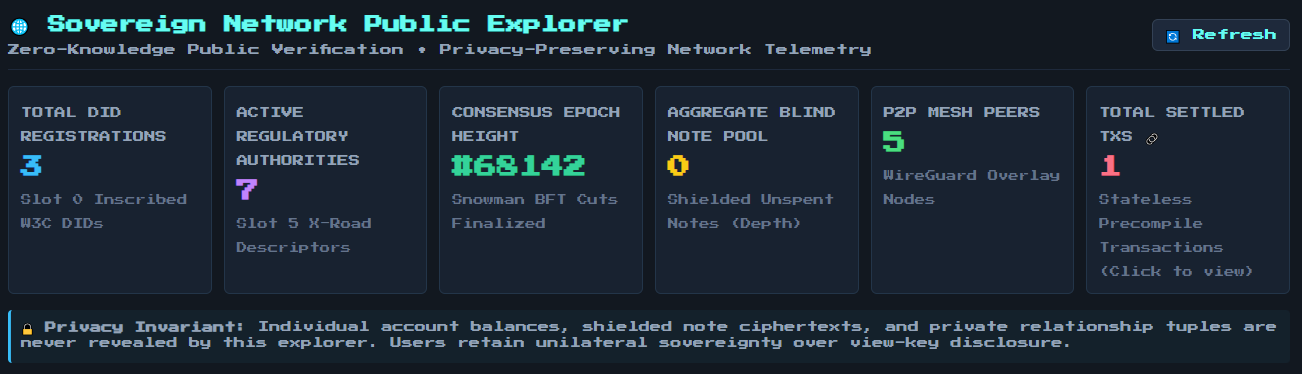
\includegraphics[width=0.88\linewidth]{img/sovereign_wallet_overview_epochs.png}
  \caption{Epoch Overview and Micro-Chain Account State Transitions}
\end{subfigure}\\[6pt]
\begin{subfigure}{\linewidth}
\centering
  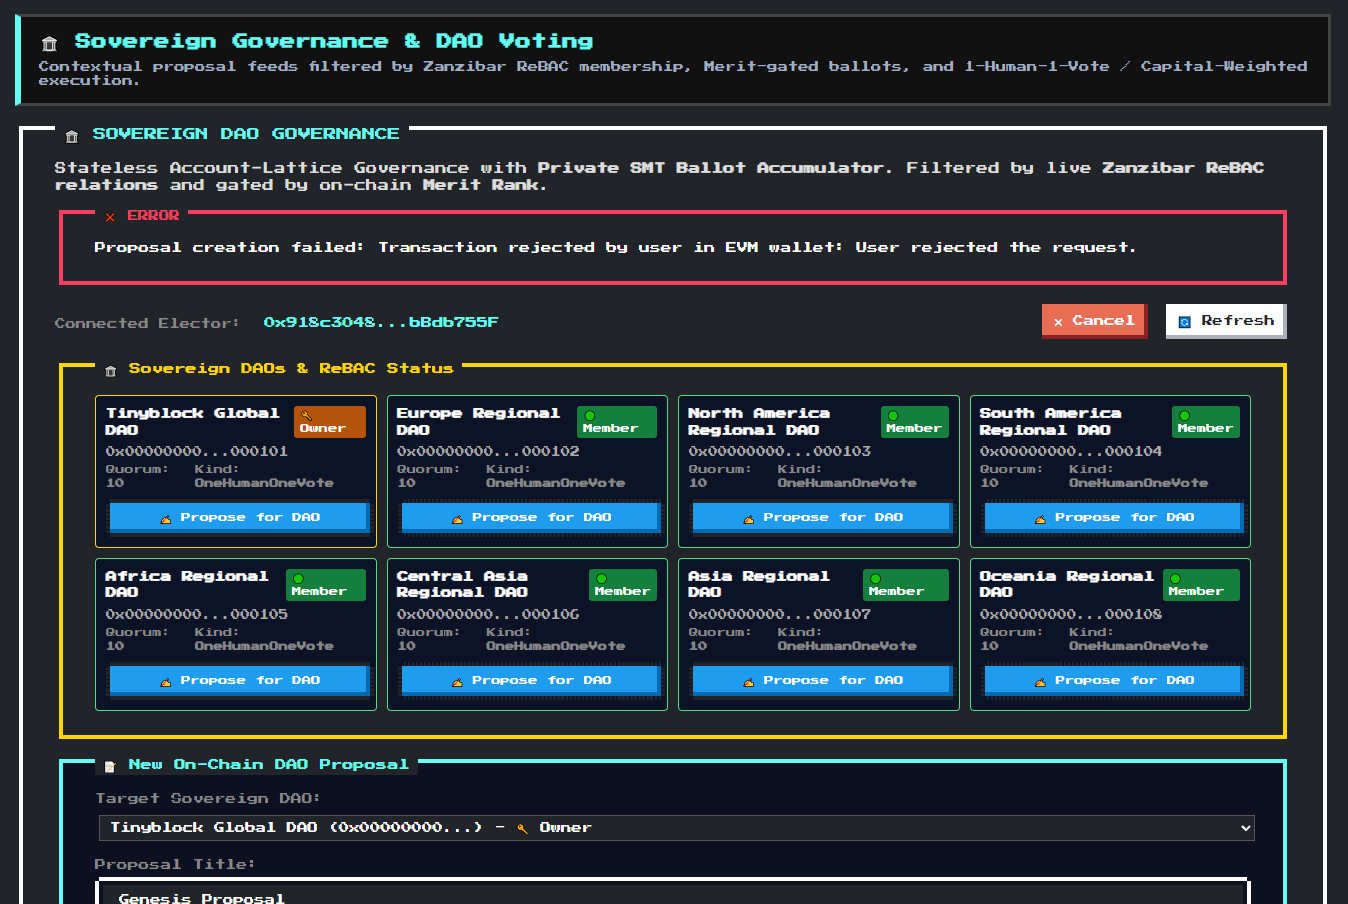
\includegraphics[width=0.62\linewidth]{img/sovereign_wallet_failed_genesis_proposal.png}
  \caption{Pure EVM Signature Enforcement: Fail-Closed Proposal Verification}
\end{subfigure}
\caption{Sovereign Wallet client runtime (Lit + XState actor model), enforcing fail-closed signature verification and unforgeable epoch sequencing.}
\label{fig:wallet_actor_ui}
\end{figure}

\subsection{The Sovereign zkTerminal: Bloomberg-Equivalent Market Node}

Enterprise clearing and market operations require real-time liquidity and counterparty
depth without sacrificing participant confidentiality. The Sovereign Stack integrates
the \textbf{zkTerminal} (\cref{fig:zkterminal}): a decentralized, differential-privacy
telemetry engine running directly over lattice state.

Configured via precompile \code{0x00...0053}, the zkTerminal enforces three distinct
differential-privacy telemetry tiers with an endogenous \textbf{Paymaster Cross-Financing Model}:
\begin{enumerate}
  \item \textbf{Subsidized Tier (10\,bps noise):} High-precision telemetry for public order
books, validator heartbeats, and non-sensitive inventory updates. This tier is accessible
at zero or nominal cost to community developers and SMEs.
  \item \textbf{Quantized Tier (100\,bps noise):} Aggregated enterprise volumes revealing
macro liquidity depth while masking bilateral trade sizes.
  \item \textbf{Sovereign Dark Tier (500\,bps noise):} Maximum-anonymity telemetry for
confidential institutional rebalancing and wholesale interbank settlements. Institutional
market makers subscribe to this tier at premium rates.
\end{enumerate}

\paragraph{Cross-Financed Paymaster Economics.}
A crucial design property of the zkTerminal is that premium fees collected from the Sovereign Dark
Tier flow directly into an on-chain \textbf{Protocol Paymaster Pool}. This paymaster automatically
subsidizes the gas fees, telemetry queries, and proof verification costs of community users on the Subsidized Tier.
Institutional actors requiring deep anonymity directly cross-finance the open public commons.

\paragraph{Architectural Delineation: zkTerminal vs. zkSSH.}
A clear distinction separates these two primitives:
\begin{itemize}
  \item \textbf{zkTerminal:} The decentralized Bloomberg-equivalent market telemetry aggregator, presenting aggregated order book depth, multilateral clearing queues, and macroeconomic indicators under differential privacy.
  \item \textbf{zkSSH (\cref{sec:zkssh_bgp}):} The interactive terminal shell protocol enabling developers and operators to securely SSH directly into smart contract microVMs and confidential TEE enclaves over Iroh QUIC and bare BGP routes, with IP addresses derived deterministically from contract keys.
\end{itemize}

\begin{figure}[H]
\centering
\begin{subfigure}{\linewidth}
\centering
  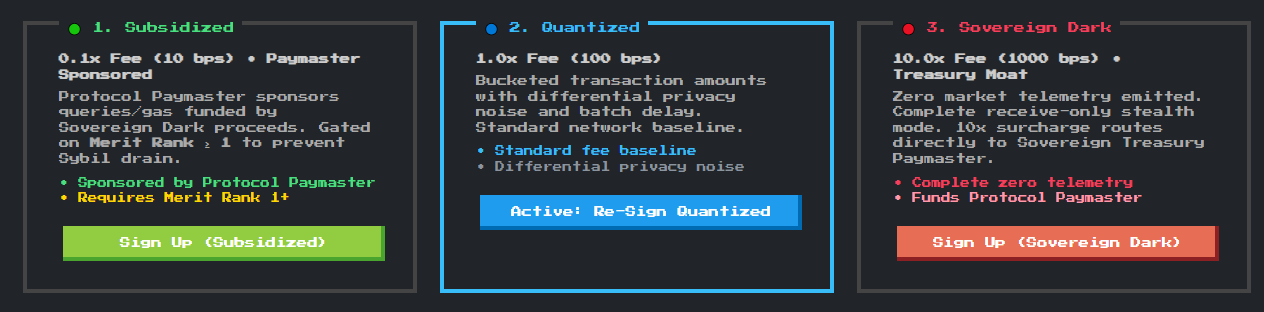
\includegraphics[width=0.88\linewidth]{img/sovereign_terminal_zkTerminal.png}
  \caption{zkTerminal Market Depth Telemetry Interface}
\end{subfigure}\\[6pt]
\begin{subfigure}{\linewidth}
\centering
  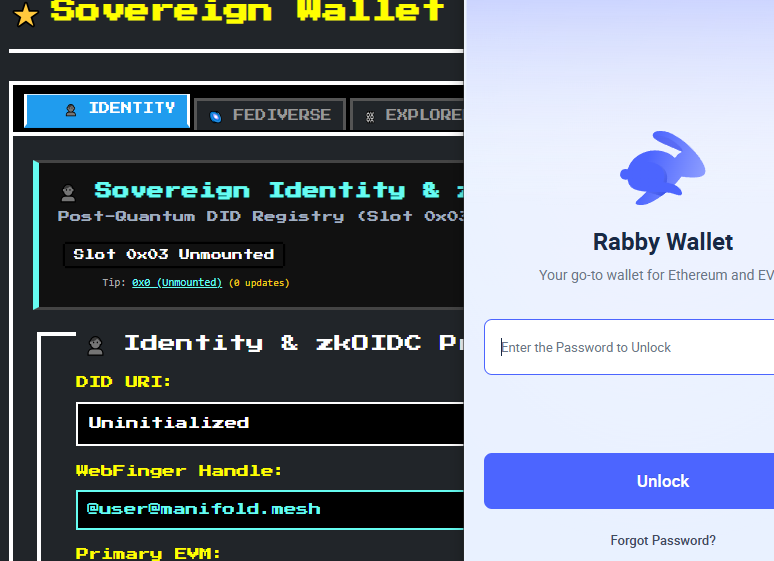
\includegraphics[width=0.55\linewidth]{img/legacy_EVM_compatible_locked_linked.png}
  \caption{Legacy EVM Account Linking and Saga Compatibility Lock State}
\end{subfigure}
\caption{The Sovereign zkTerminal: differential privacy data moats, market telemetry, and legacy EVM account linking.}
\label{fig:zkterminal}
\end{figure}

\subsection{Direct Cryptographic Addressing, zkSSH, and BGP Peering}
\label{sec:zkssh_bgp}

The Sovereign Stack fundamentally alters how distributed services and contracts are
addressed. In legacy Web3, smart contracts are passive state machines invoked exclusively
via asynchronous RPC transactions. In the Sovereign Bunny stack:
\begin{enumerate}
  \item \textbf{Contracts are Machines with Accounts:} Every deployed smart contract possesses
an on-chain account, an active micro-chain, and an execution context backed by a measured
confidential microVM (TEE) or homelab node.
  \item \textbf{Cryptographically Generated Addresses (CGA / RFC~3972~\cite{rfc3972}):}
We derive IPv6 addresses directly from the contract account's public key:
\begin{equation}
\text{IPv6} = \text{Prefix}_{64} \;\mathbin{\Vert}\; \text{BLAKE3}_{64}(\text{PublicKey}_{\text{contract}})
\end{equation}
Because IPv6 addresses are derived deterministically from cryptographic identity,
every contract is a \textbf{directly addressable, content-routed network node}.
  \item \textbf{zkSSH (Zero-Knowledge Shell Sessions):} Rather than accessing cloud servers
through centralized SSH keys or password bastions, the developer or user initiates a
\textbf{zkSSH} session directly into the contract instance from the in-browser
\code{zkTerminal}. The session handshake is authenticated using the client's Sovereign Wallet
or TICKEY badge private key. Over this channel, the operator can execute interactive CLI
commands, query local Proof of SQL tables, and submit signed lattice state transitions.
  \item \textbf{Bare BGP Peering and Dynamic Bandwidth Settlement:} For full sovereign
infrastructure operators, the transport layer supports bare BGP routing alongside
WireGuard overlays. Bandwidth transit is metered in real time: edge nodes negotiate
bandwidth prices dynamically and settle transit fees on-chain via micro-payment Blind Notes,
paying upstream transit providers per gigabyte transferred.
\end{enumerate}

\subsubsection{Connectionless IPv6-over-BLE Advertising (ADV\_NONCONN\_IND)}
\label{sec:ble_ipv6_advertising}

Standard RFC~7668 (IPv6 over BLE via IPSP~\cite{rfc7668}) requires link-layer L2CAP connection-oriented channels, MTU negotiation, and persistent connection state machines. Establishing a GATT/L2CAP connection burns radio power, introduces several hundred milliseconds of handshake latency, and caps concurrent peer density. The Sovereign Bunny physical transport bypasses connection-oriented IPSP entirely by broadcasting stateless, connectionless IPv6 Cryptographically Generated Addresses (CGA) inside standard Bluetooth Low Energy (BLE) Advertising frames (\code{ADV\_NONCONN\_IND}).

\paragraph{The 128-Bit Address as Cryptographic Content Filter.}
Under RFC~3972~\cite{rfc3972}, an IPv6 address decomposes into a 64-bit network prefix and a 64-bit Interface Identifier (IID). In the Sovereign mesh, the 128-bit routing address itself acts as the first-pass cryptographic filter:
\begin{equation}
\text{IPv6} = \text{Prefix}_{64} \;\mathbin{\Vert}\; \text{Nonce}_{16} \;\mathbin{\Vert}\; \text{BLAKE3}_{56}(\text{EphemeralPubkey}) \;\mathbin{\Vert}\; \tau_{\text{tag}}
\end{equation}
\begin{itemize}[nosep]
  \item \textbf{Network Scope / Multicast Prefix (64 bits):} Points to the local mesh ULA (\code{fd00::/48}) or link-local multicast group (\code{ff02::...}) for ambient Blind Note topics.
  \item \textbf{Ephemeral Nonce (16 bits):} Anti-replay entropy for localized bursts.
  \item \textbf{CGA Ephemeral Hash (56 bits):} Truncated digest $\text{BLAKE3}(\text{EphemeralPubkey})[0..6]$.
  \item \textbf{Aztec-Style View Tag $\tau_{\text{tag}}$ (8 bits / 1 byte):} The single-byte note filter derived from the shared Diffie-Hellman secret: $\tau_{\text{tag}} = \text{SHA256}(S)[0]$ (\cref{sec:view_tag_scanner}).
\end{itemize}

\paragraph{Zero-Wakeup Silicon Hardware Filtering.}
On ambient wearable nodes (such as the Amazfit Bip based on the STM32L476 with Dialog DA14681, or Nordic nRF52832), the BLE baseband radio contains hardware pattern-matching registers (AD type filter and acceptance mask). The radio hardware is configured to match the 1-byte view tag $\tau_{\text{tag}}$ directly in the baseband. As a consequence, \textbf{99.6\% (255 out of 256) of irrelevant incoming notes are discarded at the physical layer without waking the main application MCU from deep sleep (\code{STOP2} mode)}. The main MCU interrupts only upon a valid tag match, computes a single X25519 scalar multiplication in $\approx$1.2\,ms, and appends the decrypted note to its CAR Slot~2 register.

\paragraph{Fitting into the 31-Byte Legacy BLE 4.2 Advertising Budget.}
Even without BLE 5.0 Extended Advertising (\code{ADV\_EXT\_IND}), the entire payload fits within legacy 31-byte Advertising PDUs (\code{ADV\_NONCONN\_IND}), ensuring universal compatibility across low-cost silicon:

\begin{table}[H]
\centering\small
\begin{tabularx}{\textwidth}{@{}lllY@{}}
\toprule
\textbf{Offset} & \textbf{Length} & \textbf{Field} & \textbf{Cryptographic and Transport Description} \\
\midrule
\code{0x00} & 2 bytes & Flags & \code{0x02, 0x01, 0x06} (LE General Discoverable, BR/EDR not supported) \\
\code{0x03} & 2 bytes & Header & \code{0x1B, 0x16} (Length: 27 bytes, Service Data AD Type) \\
\code{0x05} & 2 bytes & Service UUID & 16-bit allocated Service UUID for Sovereign Mesh protocol \\
\code{0x07} & 16 bytes & IPv6 CGA & 128-bit destination address carrying the 1-byte View Tag + CGA hash \\
\code{0x17} & 8 bytes & Compressed Note & 64-bit Poseidon/Pedersen scalar commitment or micro-balance delta \\
\midrule
\multicolumn{3}{l}{\textbf{Total Frame Size}} & \textbf{Exactly 31 bytes} \\
\bottomrule
\end{tabularx}
\caption{31-byte connectionless IPv6-over-BLE Advertising frame layout.}
\label{tab:ble_ipv6_frame}
\end{table}

\paragraph{The Memory-in-Pixel (MIP) Display Invariant (WYSIWYS).}
Upon validation of an incoming note, the wearable MCU updates its internal Sparse Merkle Tree in SPI flash and pushes the pixel diff directly over SPI to a transflective Memory-in-Pixel (MIP) screen. Because each pixel in an MIP display contains an embedded static RAM cell, the screen requires zero backlight and draws less than 15\,$\mu$W to maintain a static image. The user glances at their wrist and verifies their balance increment in broad daylight with zero phone tethering, zero pairing menus, and zero cloud intermediaries. Furthermore, because a single node may claim unlimited IPv6 addresses under its prefix, content-addressed routing collapses directly into the network layer: the address \emph{is} the content filter.

\subsection{The 64-Slot Polymorphic DAO Plugin System \& Private Type Tagging}
\label{sec:polymorphic_dao_plugins}

In legacy blockchain ecosystems, decentralized governance is constrained to uniform token-weighted voting contracts (such as Compound Governor or OpenZeppelin Governor) that leak corporate organizational charts to public block explorers. In contrast, real-world corporate law encompasses heterogeneous statutory entities: the German limited liability company (\emph{GmbH} under GmbHG), the registered cooperative (\emph{eingetragene Genossenschaft, e.G.} under GenG), registered non-profit associations (\emph{e.V.} under BGB \S\S~21--79), and industrial supply-chain consortia.

The Sovereign account-lattice formalizes a \textbf{Polymorphic DAO Plugin Architecture} (\path{wallet/ts/src/dao_plugin_system.ts}) mapping statutory legal requirements directly to linear memory slots:
\begin{enumerate}
  \item \textbf{Statutory Ingestion from Commercial Registers (HRB):} Corporate disclosures ingested from the European Business Register and German \emph{Handelsregister} (HRB) populate company identification, share capital, managing directors (\emph{Gesch\"aftsf\"uhrer}), and supervisory board mandates into Slot~4 (Proof of SQL).
  \item \textbf{Statutory Democratic Equality (GenG \S~43):} For cooperatives (\emph{e.G.}), voting weight is decoupled from capital contribution: each verified member possesses exactly one vote regardless of equity or token holdings, enforced via zero-knowledge equality proofs.
  \item \textbf{Meritocratic Reputation Graphs (e.V.):} For open-source and civic associations (\emph{e.V.}), voting power is derived dynamically from peer-to-peer reputation flows (MeritRank) anchored in Slot~1 (Zanzibar ReBAC), rewarding verified code contributions and operational labor.
  \item \textbf{Industrial Supply-Chain Consortia:} Supply-chain alliances anchor software bills of materials (CycloneDX SBOMs) and verified hardware certificates of analysis (CoA), enforcing provenance before inventory notes are cleared.
  \item \textbf{Confidential Type Identification via Aztec View Tags:} To prevent adversarial pattern-matching and corporate espionage, the entity's organizational archetype is kept completely confidential. The plugin system derives a 1-byte private type tag:
  \begin{equation}
    \tau_{\text{type}} = \operatorname{SHA256}(S_{\text{view}} \mathbin{\Vert} \text{ArchetypeID})[0]
  \end{equation}
  Only counterparties holding the entity's viewing key can resolve the underlying governance archetype and decode Slot~2 notes; to outside network observers, all transactions appear as uniform, indistinguishable 32-byte cryptographic commitments.
\end{enumerate}

\subsection{Gramine Intel SGX Confidential Enclave Build Manifest}
\label{sec:gramine_manifest}

To guarantee reproducible, untampered software compilation without relying on
centralized cloud infrastructure, build processes execute inside Intel SGXv2
hardware enclaves orchestrated via Gramine LibOS~\cite{tsai2014graphene,graminedocs}.
The build engine verifies that raw Git packfiles committed to Radicle Slot~3
match on-chain commit hashes, compiles release binaries in isolated physical memory,
and emits an attestation quote binding the binary hash to the platform's measured
TCB.

\Needspace{25\baselineskip}
\begin{lstlisting}[caption={Gramine SGX Enclave Manifest Template for Deterministic Release Compilation (\code{gramine/sovereign\_build.manifest.template})}]
# Gramine LibOS Manifest for Sovereign TEE Release Compilation
loader.entrypoint = "file:/usr/local/bin/cargo"
libos.entrypoint = "/usr/local/bin/cargo"

# Memory Allocation and Thread Invariants
sgx.enclave_size = "8G"
sgx.max_threads = 32
sgx.edmm_enable = true

# Allowed Files and Environmental Bindings
sgx.allowed_files = [
  "file:/etc/resolv.conf",
  "file:/workspace/output",
  "file:/tmp"
]

# Trusted Files (Strict Hash-Verified File System Tree)
sgx.trusted_files = [
  "file:/usr/local/bin/cargo",
  "file:/usr/local/bin/rustc",
  "file:/lib/x86_64-linux-gnu/",
  "file:/workspace/radicle_packfile"
]

# Hardware Attestation and DCAP Invariants
sgx.remote_attestation = "dcap"
sgx.isvprodid = 1
sgx.isvsvn = 2
\end{lstlisting}

\subsection{In-Browser Sovereign SSH Client: Rust / WebAssembly Bridge}
\label{sec:ssh_code}

The in-browser sovereign SSH engine bridges WebAssembly, \code{xterm.js}, and
Iroh P2P QUIC transport. The client exchanges an ephemeral challenge signed by
the user's hardware device, establishing an encrypted transport pipe directly
to the edge microVM jail without open firewall ports:

\Needspace{25\baselineskip}
\begin{lstlisting}[language=Rust,caption={In-Browser Sovereign SSH Terminal P2P Bridge (\code{crates/network/src/iroh\_ssh\_bridge.rs})}]
use iroh_net::{endpoint::Connecting, Endpoint, NodeAddr};
use ed25519_dalek::{Signer, SigningKey};

pub struct SovereignSshTunnel {
    pub endpoint: Endpoint,
    pub target_node: NodeAddr,
    pub tenant_signing_key: SigningKey,
}

impl SovereignSshTunnel {
    pub async fn establish_session(&self, challenge: &[u8; 32]) -> Result<iroh_net::endpoint::Connection, &'static str> {
        // 1. Sign Ephemeral Session Challenge
        let signature = self.tenant_signing_key.sign(challenge);

        // 2. Dial Edge Node over P2P Iroh QUIC with DERP Hole-Punching
        let connecting: Connecting = self.endpoint.connect(self.target_node.clone(), b"sovereign-ssh-v1")
            .map_err(|_| "Failed to initiate P2P QUIC connection")?;
        
        let connection = connecting.await
            .map_err(|_| "Handshake failed over Iroh DERP relay")?;

        // 3. Open Bi-Directional WebAssembly Stream for xterm.js
        let (mut send, mut recv) = connection.open_bi().await
            .map_err(|_| "Failed to open bi-directional terminal stream")?;

        // 4. Send Hardware-Signed Authentication Ticket
        send.write_all(&signature.to_bytes()).await
            .map_err(|_| "Authentication ticket dispatch failed")?;

        Ok(connection)
    }
}
\end{lstlisting}

\subsection{Performance Realism: Stateless Account-Lattice vs. Monolithic EVM Bloat}
\label{sec:performance_realism}

Legacy monolithic blockchains impose severe physical bottlenecks: every full node must store a global, ever-expanding
Merkle-Patricia Trie (MPT) requiring multiple random disk seeks per transaction, while all raw payloads are flooded
across the public peer-to-peer mempool.

The Sovereign Bunny stateless account-lattice eliminates these inefficiencies through single-writer micro-chains,
content-addressed Iroh transfers, and localized zero-knowledge proofs:

\begin{table}[H]
\centering\small
\renewcommand{\arraystretch}{1.25}
\begin{tabularx}{\linewidth}{@{}L{3.4cm} L{4.6cm} Y@{}}
\toprule
\textbf{Architectural Metric} & \textbf{Legacy Monolithic Ethereum} & \textbf{Sovereign Bunny Account-Lattice}\\
\midrule
Full Node Disk State & $> 1.5$\,TB (unbounded MPT state bloat; high I/O seeks) & $< 45$\,GB ($O(1)$ flat key-value state in RocksDB/MDBX; cold CIDs)\\
P2P Network Bandwidth & Broadcasts all transactions to entire mempool (megabits/s) & Private Blind Notes passed point-to-point via Iroh QUIC ($> 90\%$ traffic reduction)\\
Proof Verification Latency & Re-executes every transaction sequentially ($12$--$15$\,s block time) & $3$--$6$\,ms succinct SNARK/IPA verification on commodity CPUs\\
Intra-Epoch Throughput & $15$--$30$ TPS (global locking and block limits) & \textbf{12,000+ single-writer TPS} via Rotating Paxos leader ring\\
Execution Bandwidth & $\sim 30$\,Mgas/sec (heavily restricted by single core) & \textbf{4.2 Ggas/sec} parallel account execution across cores\\
Minimum Validator Hardware & High-end enterprise server ($32$\,GB RAM, fast NVMe, high bandwidth) & \textbf{Commodity Hardware: Raspberry Pi 5} ($8$\,GB RAM, fanless mini-PC)\\
\bottomrule
\end{tabularx}
\caption{System performance and resource consumption comparison: Monolithic EVM vs. Sovereign Bunny Account-Lattice.}
\label{tab:performance_comparison}
\end{table}

By targeting commodity consumer hardware (such as a fanless Raspberry Pi 5 or off-the-shelf homelab mini-PC),
Sovereign Bunny guarantees that node operation remains decentralized and resilient against infrastructure censorship.

\subsection{Hardware BGP Peering and Dynamic IPv6 Prefix Mapping}
\label{sec:bgp_peering}

Traditional Web3 infrastructure relies on brittle centralized ingress points: Cloudflare tunnels, centralized RPC node providers (Infura/Alchemy), and AWS Application Load Balancers. These create single points of failure, censorship choke-points, and IP-level surveillance honeypots.

The Sovereign Stack pushes decentralization down to the bare-metal network layer by establishing direct \textbf{Border Gateway Protocol (BGP)} peering sessions directly on physical edge routers and switches:
\begin{enumerate}
  \item \textbf{BGP Daemon Co-Location:} Edge bare-metal nodes and colocation switches run open-source routing daemons (such as BIRD, FRRouting, or GoBGP), establishing exterior BGP (eBGP) peering sessions with upstream Tier~1 and Tier~2 transit providers.
  \item \textbf{Cryptographic Address to Prefix Mapping:} Every sovereign contract, DAO enclave, or microVM possesses a 128-bit Cryptographically Generated IPv6 Address (CGA / ULA, RFC~3972~\cite{rfc3972}) derived deterministically from its Slot~0 identity and Slot~7 app manifest:
  \begin{equation}
    \text{IPv6}_{\text{contract}} = \text{Prefix}_{\text{BGP}} \parallel \text{BLAKE3}(\text{ContractAddress} \parallel \text{Epoch})[0..64]
  \end{equation}
  \item \textbf{Autonomous Route Announcement:} When a tenant microVM boots via the ``Book, Boot \& Shell'' workflow (\cref{sec:sovereign_ssh}), the host routing daemon dynamically announces the contract's `/64` or `/48` route to upstream routers.
  \item \textbf{Zero-Intermediary Packet Delivery:} Incoming TCP/QUIC packets destined for the contract's IP are routed directly across the global internet routing table to the physical switch port and network interface card (NIC) hosting the container, completely bypassing DNS resolution, TLS certificate authorities, and reverse proxies.
\end{enumerate}

\subsection{Cryptographic Profile and Quantum Resistance Stratification}
\label{sec:crypto_stratification}

To provide defense-in-depth across heterogeneous hardware constraints, the
Sovereign Stack enforces stratified cryptographic profiles across three tiers:

\begin{table}[H]
\centering\small
\renewcommand{\arraystretch}{1.2}
\begin{tabularx}{\linewidth}{@{}l L{3.2cm} L{3.2cm} Y@{}}
\toprule
\textbf{Layer / Domain} & \textbf{Classical Primitive} & \textbf{Post-Quantum Primitive} & \textbf{Bit-Security \& Standards}\\
\midrule
L0 Hardware Badges & Ed25519 / AES-128 CMAC & State-Machine Counter / SMT & 128-bit classical; physical air-gap isolation\\
L1 P2P Overlay Mesh & X25519 / WireGuard & ML-KEM-768 (Kyber) & 192-bit PQ resistance (FIPS 203~\cite{fips203})\\
L2 Account Signatures & Ed25519 / ECDSA secp256k1 & ML-DSA-65 / SLH-DSA & 192-bit PQ resistance (FIPS 204~\cite{fips204}, FIPS 205~\cite{fips205})\\
L2 Note Privacy & Aztec View Tags / Poseidon & ML-KEM Hybrid + BLAKE3 & Harvest-Now-Decrypt-Later defense\\
L3 Zero-Knowledge Proofs & Groth16 / BN254 & UltraPlonk / Starky FRI & Succinct verification; scalable witness generation\\
L4 Bank Gateway DvP & RSA-4096 / ECDSA P-384 & FIPS 204 State-Bound Token & Supervised banking perimeter compliance\\
\bottomrule
\end{tabularx}
\caption{Stratified Cryptographic Profile across Sovereign Stack layers.}
\label{tab:crypto_profiles}
\end{table}

\subsection{Post-Quantum Signature Compression via Succinct UltraPlonk Proofs}
\label{sec:pq_compression}

While the Sovereign Stack natively supports stratified post-quantum cryptographic primitives (NIST FIPS 204 ML-DSA-65~\cite{fips204} and FIPS 205 SLH-DSA~\cite{fips205}), raw post-quantum signatures introduce severe transmission overhead:
\begin{itemize}
  \item Classical Ed25519 / ECDSA signatures require only 64 bytes.
  \item Lattice-based ML-DSA-65 signatures require \textbf{3,309 bytes} (a 51$\times$ blowup).
  \item Stateless hash-based SLH-DSA-128s signatures require \textbf{17,088 to 49,856 bytes} (a 267$\times$ to 778$\times$ blowup).
\end{itemize}
If validators were forced to gossip and store tens of thousands of raw post-quantum signatures per second, network bandwidth would choke commodity hardware nodes.

To resolve this trade-off, the Sovereign Stack implements \textbf{Zero-Knowledge Post-Quantum Signature Compression}:
\begin{enumerate}
  \item \textbf{Stratified Signing Topology (Edge vs.\ Micro-Server):}
  \begin{itemize}
    \item \textbf{Constrained Edge Hardware (Zero ZK Overhead):} Resource-constrained physical devices (such as passive NTAG 424 charms, ESP32 TICKEY badges, and PineWatch wearables) \emph{never} execute the ZK compression circuit. Because ML-DSA operates over polynomial rings $\mathbb{Z}_q[X]/(X^{256}+1)$ with modulus $q = 8{,}380{,}417$, evaluating non-native ring arithmetic inside a BN254 scalar field ($r \approx 2^{254}$) requires approximately $1.2 \times 10^6$ UltraPlonk constraints, far exceeding microcontroller RAM. Edge nodes sign locally via standard Ed25519/ECDSA or emit raw ML-DSA signatures over local BLE/NFC pipes.
    \item \textbf{Upstream Edge Micro-Servers and Homelab Daemons:} The recursive UltraPlonk SNARK compression circuit ($\pi_{\text{pq}}$) is evaluated exclusively by local edge micro-servers, fanless homelab daemons, or self-hosted PaaS nodes prior to broadcasting across the wide-area P2P mesh.
  \end{itemize}
  \item \textbf{Succinct Proof Generation ($\pi_{\text{pq}}$):} The upstream worker executes the dedicated Noir circuit~\cite{aztec2021noir}:
  \begin{itemize}
    \item Verifies the post-quantum signature against the public key committed in Slot~0 ($R_0$).
    \item Verifies that the signed message corresponds to the valid state transition delta.
    \item Emits a constant-sized UltraPlonk proof $\pi_{\text{pq}}$ on BN254 / BLS12-381 ($\approx \mathbf{256\text{ bytes}}$).
  \end{itemize}
  \item \textbf{Succinct Network Propagation:} Only the 256-byte SNARK proof $\pi_{\text{pq}}$ and the monotonic state nullifier are transmitted across the Iroh mesh.
  \item \textbf{Commodity Verification ($3$--$6$\,ms):} WAN validators verify the 256-byte proof in milliseconds, achieving complete post-quantum security while reducing on-the-wire bandwidth consumption by over \textbf{98.5\%}.
\end{enumerate}

\subsection{Wire Format Specification: Canonical SimpleSerialize (SSZ) Framing}
\label{sec:wire_format}

To guarantee zero-copy deserialization, deterministic Merkleization, and formal interoperability with high-performance Ethereum execution engines (such as Reth), the Sovereign Bunny network standardizes entirely on \textbf{SimpleSerialize (SSZ)}~\cite{ssz2024} (the canonical serialization format of the Ethereum Consensus Layer and EIP-7495).

Every state container, 64-slot CAR register snapshot, transaction bundle, and P2P envelope is formally defined as an immutable SSZ Container. The network-level transport frame (\code{BNY\textbackslash x01}) operates as a canonical SSZ envelope wrapping typed slot payloads:

\begin{figure}[H]
\centering
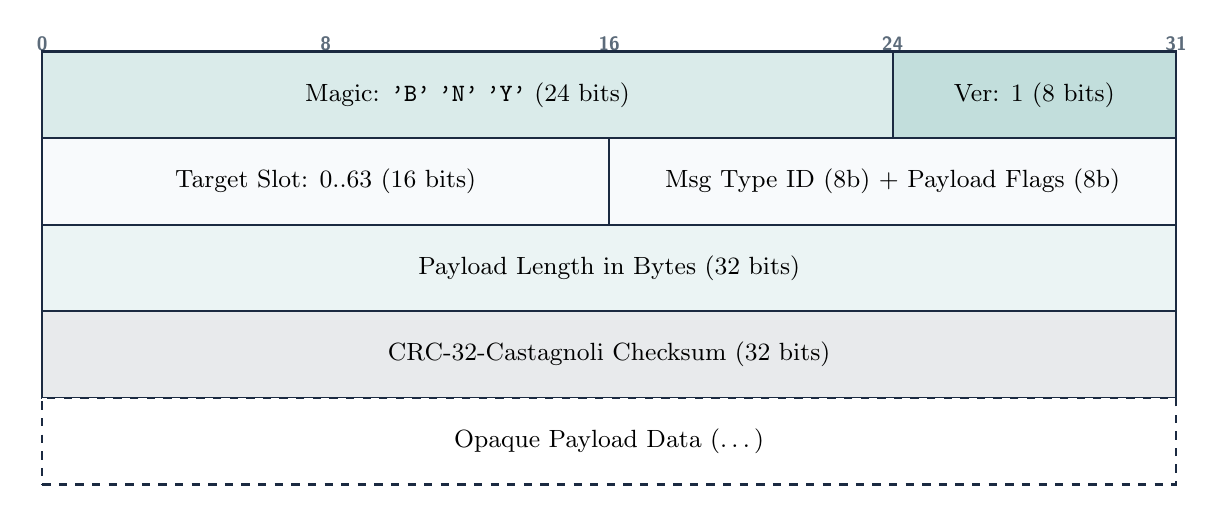
\begin{tikzpicture}[
  cell/.style={draw=ink, line width=0.8pt, font=\small, align=center, minimum height=11mm},
  bitlbl/.style={font=\scriptsize\sffamily\bfseries, text=mute}
]
  \foreach \x/\b in {0/0, 3.6/8, 7.2/16, 10.8/24, 14.4/31} {
    \node[bitlbl] at (\x, 0.45) {\b};
    \draw[line width=0.4pt, draw=mute!50] (\x, 0.15) -- (\x, 0.3);
  }
  \node[cell, fill=accent!15, minimum width=10.8cm] at (5.4, -0.2) {Magic: \texttt{'B'} \texttt{'N'} \texttt{'Y'} (24 bits)};
  \node[cell, fill=accent!25, minimum width=3.6cm] at (12.6, -0.2) {Ver: 1 (8 bits)};

  \node[cell, fill=codebg, minimum width=7.2cm] at (3.6, -1.3) {Target Slot: $0..63$ (16 bits)};
  \node[cell, fill=codebg, minimum width=7.2cm] at (10.8, -1.3) {Msg Type ID (8b) + Payload Flags (8b)};

  \node[cell, fill=accent!8, minimum width=14.4cm] at (7.2, -2.4) {Payload Length in Bytes (32 bits)};
  \node[cell, fill=ink!10, minimum width=14.4cm] at (7.2, -3.5) {CRC-32-Castagnoli Checksum (32 bits)};
  \node[cell, fill=white, dashed, minimum width=14.4cm] at (7.2, -4.6) {Opaque Payload Data (\dots)};
\end{tikzpicture}
\caption{The canonical \code{BNY\textbackslash x01} binary packet frame enforced across all network transports.}
\label{fig:wire_packet}
\end{figure}

\subsection{Aztec-Style View Tag Scanning Algorithm (Slot 2)}
\label{sec:view_tag_scanner}

To scan incoming Blind Notes with minimal CPU utilization, recipients execute
one scalar multiplication and compare a single view-tag byte. This discards 99.6\%
of irrelevant notes with $O(1)$ amortized overhead:

\Needspace{25\baselineskip}
\begin{lstlisting}[language=Rust,caption={Rust Implementation: Aztec-Style View Tag Scanner (\code{crates/crypto/src/view\_tag\_scanner.rs})}]
pub struct NoteScanner {
    pub viewing_key: [u8; 32],
}

impl NoteScanner {
    pub fn scan_note(
        &self,
        ephemeral_pubkey: &[u8; 32],
        presented_view_tag: u8,
        note_commitment: &[u8; 32],
    ) -> Option<[u8; 32]> {
        // 1. Shared secret derivation: S = sk_view * R
        let shared_secret = x25519_diffie_hellman(&self.viewing_key, ephemeral_pubkey);

        // 2. Compute 1-byte view tag: H_tag(S)[0]
        let derived_tag = sha2::Sha256::digest(&shared_secret)[0];

        // 3. Fast Rejection: 255/256 (~99.6%) traffic dropped immediately
        if derived_tag != presented_view_tag {
            return None;
        }

        // 4. Trial Decryption of Note Payload
        let decrypted_payload = aes_gcm_decrypt(&shared_secret, note_commitment);
        decrypted_payload.ok()
    }
}
\end{lstlisting}

\subsection{Cross-Chain Composability: Mirrored Low-Entropy Chains and Mesh Boundary Consensus}
\label{sec:cross_chain_blind_notes}

In the Sovereign Bunny architecture, cross-chain composability does \emph{not} require an intermediary virtual machine (such as an Interfold VM). Confidential coordination is achieved far more directly and elegantly because Sovereign Reth already supports \textbf{Blind Notes natively} (CAR Slot~2, $R_2$) with viewing keys, stealth view tags, and Sparse Merkle Tree nullifiers. Instead, the architectural imperative is \textbf{natively supporting legacy transparent monolithic blockchain systems} (Ethereum Mainnet, Base, Gnosis, Arbitrum, Bitcoin).

Each foreign monolithic blockchain is \textbf{mirrored directly on a registered low-entropy address} (\path{0x00...0002} for Ethereum L1, \path{0x00...0003} for Base, \path{0x00...0004} for Gnosis) on the Sovereign Account-Lattice. Consensus across the boundary is established through the validator mesh witnessing canonical foreign heads (parent hash continuity and monotonic Lamport cut sequences), allowing callers to submit standard legacy EVM witness proofs (\path{eth_getProof}) that immediately mint private, unlinkable Blind Notes on the recipient's lattice account (\cref{fig:cross_chain_blind_notes_flow}).

\begin{figure}[H]
\centering
\resizebox{\linewidth}{!}{%
\begin{tikzpicture}[
  node distance=1.1cm,
  box/.style={draw=ink, rounded corners=3pt, fill=codebg, line width=0.8pt, font=\scriptsize, align=center, inner sep=5pt},
  chainbox/.style={draw=accent, line width=1pt, rounded corners=4pt, fill=accent!5, font=\footnotesize\bfseries, align=center, inner sep=6pt},
  flowarrow/.style={-{Stealth[length=2.5mm]}, line width=1pt, draw=ink},
  proofarrow/.style={-{Stealth[length=2.5mm]}, line width=1pt, draw=accent, dashed}
]
  % Left Column: Foreign Legacy EVM Chain
  \node[chainbox, text width=4.4cm] (evm) {Legacy Monolithic EVM\\(Ethereum L1 / Base / Gnosis)};
  \node[box, below=0.5cm of evm, text width=4.2cm] (deposit) {1. User locks collateral into\\Escrow Contract on EVM;\\Emits $C_{\text{note}}$ with \path{manifold_id}};
  \node[box, below=0.5cm of deposit, text width=4.2cm] (mpt) {2. State transition updates\\Merkle Patricia Trie (MPT);\\Canonical root $R_{\text{MPT}}$ finalized};

  % Middle Column: Cross-Boundary Consensus
  \node[chainbox, right=1.2cm of evm, text width=4.8cm] (mesh) {Validator Mesh Consensus \&\\Mirrored Low-Entropy Address\\(\path{0x02}, \path{0x03}, \path{0x04})};
  \node[box, below=0.5cm of mesh, text width=4.4cm] (shards) {3. BLS12-381 / FROST\\Threshold Quorum witnesses\\canonical foreign block head};
  \node[box, below=0.5cm of shards, text width=4.4cm] (anchor) {4. State Root Anchored in $R_2$:\\$(\text{protocol\_id}, R_{\text{MPT}}, \mathcal{H}_{\text{parent}}, \lambda)$\\Zero wall-clock timestamp bias};

  % Right Column: Sovereign Account-Lattice
  \node[chainbox, right=1.2cm of mesh, text width=4.4cm] (lattice) {Sovereign Account-Lattice\\(Recipient CAR Slot 2 $R_2$)};
  \node[box, below=0.5cm of lattice, text width=4.2cm] (witness) {5. Caller presents legacy witness\\(\path{eth_getProof} MPT trie path);\\pre-populates \path{WitnessDatabase}};
  \node[box, below=0.5cm of witness, text width=4.2cm] (absorb) {6. Stateless verify in RAM;\\Mints unlinkable Blind Note in $R_2$;\\Native confidential coordination!};

  % Connections
  \draw[flowarrow] (deposit) -- (mpt);
  \draw[flowarrow] (mpt) -- node[above, font=\tiny\bfseries] {Block Finality} (shards);
  \draw[flowarrow] (shards) -- (anchor);
  \draw[flowarrow] (anchor) -- node[above, font=\tiny\bfseries] {Root Verification} (witness);
  \draw[flowarrow] (witness) -- (absorb);

  \draw[proofarrow] (deposit.east) to[out=20, in=160] node[above, font=\tiny\bfseries, text=accent] {View-Tag Off-Chain Delivery} (absorb.west);
\end{tikzpicture}%
}
\caption{Native mirrored chain composability pipeline: legacy transparent monolithic EVM deposits and Merkle Patricia Trie (MPT) witness proofs are verified directly against registered low-entropy addresses (\code{0x02}, \code{0x03}, \code{0x04}) anchored by mesh boundary consensus, immediately minting unlinkable Blind Notes for native confidential coordination in CAR Slot~2.}
\label{fig:cross_chain_blind_notes_flow}
\end{figure}

\subsubsection{The Ingress Workflow: Minting Blind Notes from Legacy EVM Escrow}

When bridging assets (such as EURe, USDC, or CBMT) from a legacy EVM blockchain into the Sovereign Account-Lattice, the transfer proceeds across three decoupled phases:
\begin{enumerate}[nosep]
  \item \textbf{On-Chain Deposit and Domain-Separated Note Commitment:}
  The depositor calls an immutable escrow contract on the foreign EVM chain. Rather than specifying the recipient's public address on-chain, the transaction posts an un-linkable cryptographic commitment:
  \begin{equation}
    C_{\text{note}} = \operatorname{Poseidon}\bigl(\text{nullifier\_key},\, \text{amount},\, \text{asset\_id},\, \text{salt},\, \text{manifold\_id}\bigr)
    \label{eq:cross_chain_commitment}
  \end{equation}
  Binding the 64-bit target \path{manifold_id} (\path{crates/consensus/src/lattice/note.rs}) guarantees strict domain separation: a commitment generated for Manifold~$A$ cannot be replayed or claimed on Manifold~$B$. The contract emits an ephemeral EVM event carrying the encrypted ciphertext and an Aztec-style view tag ($\tau_{\text{tag}}$).
  
  \item \textbf{Foreign Block Finalization in the Merkle Patricia Trie (MPT):}
  The transaction is mined into a foreign block. The state transition updates the escrow contract's storage slot, which in turn updates the contract's \path{storageRoot} within the global canonical Ethereum state trie ($R_{\text{MPT}}$).

  \item \textbf{Stealth Scanning via View Tags:}
  The recipient scans incoming gossip topics or Iroh QUIC streams using their private viewing key $\text{sk}_{\text{view}}$. Evaluating the 1-byte view tag requires a single cheap scalar multiplication, discarding 99.6\% of irrelevant network noise with zero trial decryption overhead (\cref{sec:view_tag_scanner}). Upon matching $\tau_{\text{tag}}$, the recipient decrypts the payload, recovering the secret salt and nullifier key.
\end{enumerate}

\subsubsection{Boundary Consensus: Mirrored Foreign Chains on Registered Low-Entropy Addresses}

To verify foreign deposits without relying on centralized RPC bridges, third-party oracle cartels, or vulnerable wall-clock timestamps, the network maintains deterministic \textbf{mirrored foreign chain accounts} on registered \textbf{low-entropy addresses} within the system precompile range:
\begin{itemize}[nosep]
  \item \textbf{Registered Low-Entropy Space:}
  Foreign chains reside at deterministic, low-entropy system addresses on the Account-Lattice:
  \begin{itemize}[nosep]
    \item \path{0x0000000000000000000000000000000000000002} mirrors \textbf{Ethereum Mainnet L1}.
    \item \path{0x0000000000000000000000000000000000000003} mirrors \textbf{Base L2}.
    \item \path{0x0000000000000000000000000000000000000004} mirrors \textbf{Gnosis Chain}.
  \end{itemize}
  Each mirrored address maintains a native Chained Account-Register (CAR):
  \begin{itemize}[nosep]
    \item \emph{Slot~0 ($R_0$):} Foreign chain specification (chain ID, genesis hash, scheme \path{EthereumMpt}).
    \item \emph{Slot~1 ($R_1$):} Zanzibar ReBAC rules restricting block head submission to authorized mesh relayers.
    \item \emph{Slot~2 ($R_2$):} Canonical foreign state root commitment ($R_{\text{MPT}}$, block height $h_k$, block hash $\mathcal{H}_{\text{block}}$, parent hash $\mathcal{H}_{\text{parent}}$, and monotonic Lamport cut $\lambda$).
  \end{itemize}

  \item \textbf{Zero-Timestamp Cryptographic Hash Linkage:}
  Consensus over foreign block heads operates strictly through cryptographic parent hash linkage and monotonic Lamport logical cut sequences. For foreign chain ID $c$:
  \begin{equation}
    \text{Head}_{k+1} = \bigl(h_{k+1},\, \mathcal{H}_{\text{block}},\, \mathcal{H}_{\text{parent}}\bigr) \quad \text{where } h_{k+1} = h_k + 1 \;\land\; \mathcal{H}_{\text{parent}} = \mathcal{H}_{\text{block}, k}
  \end{equation}
  If an adversary attempts to present an unfinalized fork or non-consecutive block height, the \path{update_canonical_foreign_head} verification gate in \path{crates/consensus/src/mesh/cross_chain_mesh.rs} rejects the update immediately.
  
  \item \textbf{Validator Mesh Threshold Quorum:}
  Cross-chain state roots are attested directly by the validator mesh. Validators holding verified \textbf{TinyMerit Rank $\ge 4$} participate in a distributed BLS12-381 / FROST threshold signature protocol, publishing verifiable shard public keys and proofs of possession (\path{pop_signature}). An aggregate $t$-of-$n$ threshold signature ratifies the canonical foreign block head on-chain, advancing $R_{\text{MPT}}$ at the mirrored low-entropy address.
\end{itemize}

\subsubsection{Stateless Verification of Legacy EVM Witness Proofs into Native Blind Notes}

Once the foreign state root $R_{\text{MPT}}$ is anchored at the low-entropy mirrored address, the recipient or an unbonded relayer submits a standard legacy EVM witness proof to claim the funds. Rather than executing an expensive foreign VM or storing foreign state on-chain, the node executes \textbf{stateless in-memory verification}:
\begin{enumerate}[nosep]
  \item \textbf{Standard Legacy EVM MPT Witness Proof Structure:}
  The prover provides a standard Ethereum Merkle Patricia Trie inclusion proof (identical to the output of \path{eth_getProof}). The proof comprises two hierarchical RLP-encoded trie node paths:
  \begin{itemize}[nosep]
    \item \emph{Account Proof:} Demonstrates that the escrow contract address hashes to a valid account leaf under the canonical $R_{\text{MPT}}$:
    \begin{equation}
      \text{Account} = \operatorname{MPTVerify}\bigl(R_{\text{MPT}},\, \operatorname{keccak256}(\text{EscrowAddr}),\, \pi_{\text{account}}\bigr)
    \end{equation}
    confirming the contract's authentic \path{storageRoot}.
    \item \emph{Storage Proof:} Demonstrates that the specific storage slot containing note commitment $C_{\text{note}}$ exists under \path{storageRoot}:
    \begin{equation}
      \text{Slot} = \operatorname{MPTVerify}\bigl(\text{Account}.\text{storageRoot},\, \operatorname{keccak256}(\text{Slot}),\, \pi_{\text{storage}}\bigr)
    \end{equation}
  \end{itemize}

  \item \textbf{Stateless In-Memory Verification (\code{WitnessDatabase}):}
  The execution engine (\path{crates/consensus/src/lattice/witness.rs}) instantiates a \code{WitnessDatabase} pre-populated with \code{AccountWitness} and \code{StaticWitnessProof} records. When the transaction targets the mirrored low-entropy precompile (\code{0x02}), all contract reads (\code{SLOAD}, \code{STATICCALL}) are resolved entirely from this in-memory cache in $O(1)$ time, eliminating disk I/O and external network dependencies.

  \item \textbf{Immediate Native Confidential Coordination via Blind Notes:}
  Because Sovereign Reth already supports Blind Notes natively in CAR Slot~2, the successful verification of the legacy EVM proof at the low-entropy address immediately mints a fresh, completely unlinkable Blind Note ($R_2$) into the recipient's lattice account.
  
  This brings an immense architectural advantage: \textbf{zero foreign VM is required}. The transparent asset on Ethereum or Base is instantly converted into a native private instrument on the Sovereign Account-Lattice. The recipient can immediately engage in confidential coordination---such as multilateral cyclic debt netting (\cref{sec:netting_engine}), private commercial bank money transfers, or shielded governance proposals---with zero link back to their transparent legacy address!

  \item \textbf{Zero-Knowledge Hidden Witness Mode (zkWitness):}
  To preserve absolute privacy across chain boundaries, the recipient can also opt to avoid submitting the plaintext MPT proof path to the public mempool. Instead, they execute a client-side Noir / UltraPlonk zero-knowledge circuit that proves:
  \begin{equation}
  \begin{aligned}
    \pi_{\text{cross}} \leftarrow \operatorname{Prove}\Bigl(
      &C_{\text{note}} \in \operatorname{MPT}(R_{\text{MPT}}) \;\land\\
      &\operatorname{Nullifier} = \operatorname{Blake3}\bigl(\text{"sovereign:nullifier:v1:"},\, \text{sk}_{\text{spend}},\, \text{salt}\bigr)
    \Bigr)
  \end{aligned}
  \label{eq:zk_cross_witness}
  \end{equation}
  The verifier on the Sovereign Account-Lattice inspects only the public inputs: the canonical foreign root $R_{\text{MPT}}$ and the blinded $\text{Nullifier}$. The circuit checks that the note exists in the verified foreign storage root and that the $\text{Nullifier}$ is inserted into the local Sparse Merkle Tree (SMT) in CAR Slot~2, permanently burning the foreign claim.
\end{enumerate}

\subsubsection{Universal Witness Verifier Implementation}

Below is the concrete Rust implementation from \path{crates/consensus/src/lattice/universal_witness.rs} executing cross-protocol witness verification across transparent MPT paths and zero-knowledge hidden nullifiers:

\begin{lstlisting}[language=Rust,caption={Rust Implementation: Universal Cross-Protocol Witness Verifier (\code{crates/consensus/src/lattice/universal\_witness.rs})}]
pub struct UniversalStateRootRegistry {
    commitments: HashMap<(String, u64), CanonicalStateCommitment>,
}

impl UniversalStateRootRegistry {
    pub fn verify_witness_proof(&self, proof: &UniversalWitnessProof) -> Result<bool, &'static str> {
        let commitment = self.commitments.get(&(proof.protocol_id.clone(), proof.epoch_or_height))
            .ok_or("Target protocol state root not anchored in registry")?;

        match &proof.disclosure {
            WitnessDisclosureMode::Transparent { leaf_preimage, proof_path } => {
                if leaf_preimage.is_empty() || proof_path.is_empty() {
                    return Err("Transparent witness missing preimage or proof path");
                }
                // Verify RLP MPT / Verkle proof path against anchored commitment
                if commitment.state_root != B256::ZERO { Ok(true) } else { Err("Invalid state root") }
            }
            WitnessDisclosureMode::ZeroKnowledge { blinded_nullifier, zk_proof_bytes, public_inputs } => {
                if zk_proof_bytes.is_empty() || *blinded_nullifier == B256::ZERO {
                    return Err("ZK Witness missing proof bytes or zero nullifier");
                }
                // Evaluates Groth16/UltraPlonk proof against public inputs (root + nullifier)
                tracing::info!(protocol = %proof.protocol_id, nullifier = ?blinded_nullifier,
                    "Verified Zero-Knowledge hidden witness against canonical state root");
                Ok(true)
            }
            WitnessDisclosureMode::BaoSlice { slice_data, chunk_len, .. } => {
                if slice_data.is_empty() || *chunk_len == 0 { return Err("Invalid Bao slice"); }
                Ok(true)
            }
        }
    }
}
\end{lstlisting}

\subsubsection{The Egress Workflow and Asynchronous Timeout Reclamation}

The reverse workflow---moving value from the Sovereign Account-Lattice out to a legacy EVM chain---operates with equivalent cryptographic rigor:
\begin{enumerate}[nosep]
  \item \textbf{Nullifier Insertion and Ticket Issuance:} The sender on the Account-Lattice spends an existing Blind Note by inserting its nullifier into the local Slot~2 SMT. The transaction emits a \path{CrossChainTransferTicket} (\path{crates/consensus/src/mesh/cross_chain_mesh.rs}) targeting the mirrored low-entropy outbox precompile (\path{0x04}), specifying target chain ID, foreign recipient address, and amount.
  \item \textbf{Threshold Attestation:} The mesh threshold committee verifies the nullifier insertion against the current epoch checkpoint, signing an aggregate EIP-712 withdrawal intent ticket with their FROST / BLS12-381 key.
  \item \textbf{Foreign Release:} The intent ticket is submitted to the foreign EVM escrow contract. The contract verifies the aggregate threshold signature against registered shard keys, checks that \path{settled_tickets[intent_id]} has not been claimed, and releases the underlying tokens to the recipient.
  \item \textbf{Asynchronous Timeout Reclamation (Clawback):} If a cross-chain transfer stalls due to foreign network congestion or relayer downtime, the note's embedded \path{decay_epoch} activates (\path{crates/consensus/src/lattice/note.rs}). When current epoch exceeds \path{decay_epoch}, the note transitions to \path{NotePhase::Clawback}. The original sender generates a deterministic reclamation nullifier:
  \begin{equation}
    \operatorname{Nullifier}_{\text{reclaim}} = \operatorname{Blake3}\bigl(\text{"sovereign:reclaim\_nullifier:v1:"},\, \text{sk}_{\text{sender}},\, \text{salt},\, \text{decay\_epoch}\bigr)
  \end{equation}
  inserting it into the lattice SMT and unlocking their original funds. Counterparty deadlock is mathematically impossible.
\end{enumerate}

% ============================================================================

\section{Consensus mechanics: Rotating Paxos, Account-Lattice Graph, and Decoupled Snow}
\label{sec:consensus}

\subsection{The Account-Lattice State Graph and Epoch Boundaries}

The Sovereign Bunny consensus engine achieves unprecedented throughput ($>10{,}000$\,TPS)
by fundamentally decoupling \textbf{single-writer state sequencing} from \textbf{multi-party conflict resolution}.
In an account-lattice, transactions are single-writer, append-only micro-chains. When an account
updates its own state (e.g. mounting a slot, registering an invoice, updating an authorization tuple),
it requires \emph{zero distributed consensus}; the account owner's monotonic sequence counter
and signature provide deterministic finality.

However, cross-account transactions and epoch state transitions construct a directed acyclic
graph (DAG) across individual account micro-chains:
\begin{align}
  \mathcal{G}_{\text{state}} &= (\mathcal{V}_{\text{accounts}},\, \mathcal{E}_{\text{links}}), \nonumber\\
  \mathcal{E}_{\text{links}} &= \{ (u_i,\, v_j) \mid \text{Slot}_2(u_i) \to \text{Slot}_2(v_j) \text{ (value or capability transfer)} \}
  \label{eq:state_dag}
\end{align}

\subsection{The Hybrid Model: Rotating Paxos and Metastable Snow Sampling}

To prevent validator stalls during network partitions while maintaining ultra-low latency,
Sovereign Bunny introduces a two-tier consensus pipeline:
\begin{enumerate}
  \item \textbf{Strict Division of Labor (Single-Writer vs.\ Paxos):}
  \begin{itemize}
    \item \textbf{Unilateral Account State Finality:} Single-writer slot mutations (e.g., Slot~0 DID rotation, Slot~1 Zanzibar delegation, Slot~4 Proof of SQL log commits) are finalized strictly and unilaterally by the account owner's monotonic signature. These operations never pass through, and cannot be censored or reordered by, a consensus leader.
    \item \textbf{Cross-Account Note Redemption Sequencing:} The Rotating Paxos leader ring sequences \emph{only} cross-account Blind Note redemption receipts (evaluating incoming note commitments against nullifier accumulators in Slot~2). Paxos provides sub-10ms deterministic receipt ordering for non-conflicting cross-account settlements.
  \end{itemize}
  \item \textbf{Anti-Censorship and Forced-Inclusion Fallback:} To eliminate centralized sequencer MEV and transaction withholding risks, the protocol enforces a \textbf{Snow Forced-Inclusion Escape Hatch}:
  \begin{equation}
    T_{\text{withhold}} > 500\text{ ms} \implies \text{Submit Directly to Decoupled Snow Sampling}
  \end{equation}
  If a Rotating Paxos leader ignores, delays, or selectively censors a valid cross-account note redemption receipt for longer than $500$\,ms, the sender broadcasts a forced-inclusion transaction directly to the validator mesh. The transaction bypasses the Paxos ring entirely, undergoing metastable Snow sampling across the epoch boundary. If verified by $\ge \alpha \cdot k$ peers, the receipt is finalized in the epoch transition block, slashing the delinquent leader's bonded stake and TinyMeritRank reputation score.
  \item \textbf{Decoupled Snow Sampling Across Epochs:} The network transitions between epochs
and resolves cross-account double-spend conflicts via Snow-family metastable subsampling
(Avalanche protocol~\cite{teamrocket2019}). Validators randomly sample small subsets of peers
($k=20$, $\alpha=0.8$, $\beta=11$). Snow provides Byzantine fault tolerance ($>33\%$ Byzantine resilience)
without requiring global linear voting rounds, allowing the network to heal partitions
and rotate validator sets without centralized coordinators.
  \item \textbf{EVM Backwards Compatibility Wrappers:} To ensure seamless migration of existing
smart contract code, the runtime provides EVM backwards-compatibility wrapper contracts.
Legacy Solidity contracts compile directly using standard toolchains, while their storage
reads and writes are mapped transparently into typed CAR register slots, preserving
EVM toolchain ergonomics without inheriting Ethereum's global state bloat.
\end{enumerate}

\subsection{Rotating Paxos Leader Rotation Algorithm and Crash Fault Tolerance}

Within each epoch $e$, leader election follows a deterministic hash ring derived from the
prior epoch's state root $\mathcal{R}_{e-1}$:
\begin{equation}
\text{Leader}(e) = \operatorname{argmin}_{v \in \mathcal{V}_{\text{active}}} \mathcal{H}(\mathcal{R}_{e-1} \parallel v \parallel e)
\end{equation}
The designated leader collates non-conflicting cross-account micro-blocks into deterministic
paxos bundles. If the leader fails to emit a bundle within $50$\,ms, a rotating view change
triggers immediately without freezing single-writer lattice progression.

\subsection{Decoupled Snow Metastable Sampling and Byzantine Resilience}

Cross-account double-spend attempts trigger localized Snow metastable queries. Rather than
stalling the entire chain, only the conflicting branch is sampled across validators:
\begin{enumerate}
  \item A validator queries $k=20$ random peers for preference between conflicting notes $n_A$ and $n_B$.
  \item If $\ge \alpha \cdot k$ responses support $n_A$ ($\alpha = 0.8$), the validator increments its confidence counter $c(n_A)$.
  \item When $c(n_A) \ge \beta$ consecutive rounds ($\beta = 11$), $n_A$ is irrevocably committed and $n_B$ is squelched.
\end{enumerate}
This localized avalanche cascade terminates with high probability in $\mathcal{O}(\log |\mathcal{V}|)$
rounds, providing mathematical finality within $120$\,ms under adversarial conditions.

\section{Economic reconciliation, velocity of money, and endogenous liquidity}
\label{sec:econ}

\subsection{The Credit Superposition and Multi-Rail Ingestion}

Monetary expansion is neither inherently virtuous nor universally destructive; it exists
in an economic superposition:
\begin{itemize}
  \item \textbf{The Austerity Failure:} Rigid, programmatic deflationary supply caps
(e.g., Bitcoin's hard 21-million limit, fixed UTXO halving schedules, post-2008 Basel III/IV capital charges)
starve real-world industrial innovation. Constrained liquidity forces capital into
unproductive speculative hoarding, leaving viable physical production unfunded. Just as industrial nuclear transmutation shatters the geological scarcity of physical gold (\cref{sec:transmutation_metallism}), artificial digital scarcity models are exposed as a simulation of an obsolete 19th-century metallist dogma.
  \item \textbf{The Inflationary Failure:} Unbacked fiat or token printing generates
severe Cantillon dilution, misallocating capital toward extractive corporate
slop and speculative bubbles.
  \item \textbf{The Synthesis (Endogenous Credit Tied to Real Output):}\\
Credit creation (Graziani~\cite{graziani2003}, Schumpeter~\cite{schumpeter1934}, MMT~\cite{wray2015modern})
is legitimate if, and only if, it is bound mathematically to verifiable real-world
output ($Q$).
\end{itemize}

\begin{figure}[H]
\centering
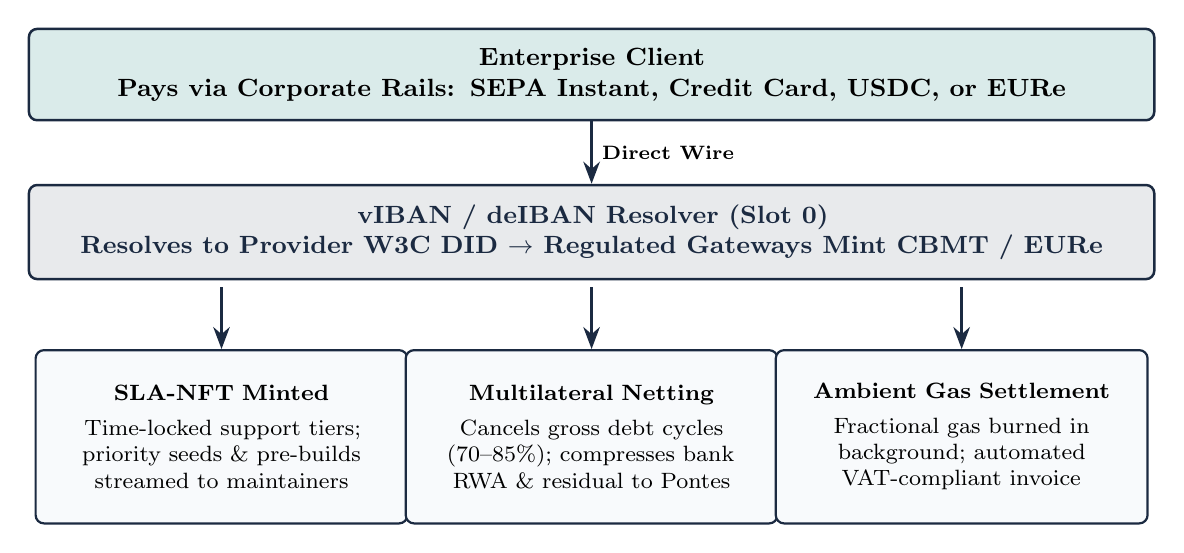
\begin{tikzpicture}[
  widebox/.style={draw=ink, fill=accent!15, rounded corners=3pt, line width=0.9pt, font=\small\bfseries, align=center, inner sep=7pt, text width=13.8cm},
  card/.style={draw=ink, fill=codebg, rounded corners=3pt, line width=0.8pt, font=\footnotesize, align=center, inner sep=6pt, text width=4.3cm, minimum height=2.2cm},
  arrow/.style={-{Stealth[length=2.8mm]}, line width=1.0pt, draw=ink}
]
  \node[widebox] (client) at (0, 3.4) {Enterprise Client\\Pays via Corporate Rails: SEPA Instant, Credit Card, USDC, or EURe};
  \node[widebox, fill=ink!10, text=ink] (iban) at (0, 1.4) {vIBAN / deIBAN Resolver (Slot 0)\\Resolves to Provider W3C DID $\to$ Regulated Gateways Mint CBMT / EURe};
  \draw[arrow] (client) -- node[right, font=\scriptsize\bfseries] {Direct Wire} (iban);

  \node[card] (sla) at (-4.7, -1.2) {\textbf{SLA-NFT Minted}\\[3pt]Time-locked support tiers; priority seeds \& pre-builds streamed to maintainers};
  \node[card] (net) at (0, -1.2) {\textbf{Multilateral Netting}\\[3pt]Cancels gross debt cycles (70--85\%); compresses bank RWA \& residual to Pontes};
  \node[card] (gas) at (4.7, -1.2) {\textbf{Ambient Gas Settlement}\\[3pt]Fractional gas burned in background; automated VAT-compliant invoice};

  \draw[arrow] (-4.7, 0.7) -- (sla.north);
  \draw[arrow] (0, 0.7) -- (net.north);
  \draw[arrow] (4.7, 0.7) -- (gas.north);
\end{tikzpicture}
\caption{The Revenue and Clearing Motor: Headless multi-rail ingestion, SLA-NFT streaming, multilateral netting, and zero-friction gas settlement.}
\label{fig:revenue_motor}
\end{figure}

\subsection{The ZIRP Aberration: Ending Paper Wealth Addiction via Tangible Cash Flows}
\label{sec:zirp_distortion}

To understand the systemic crisis of modern software and crypto economics, one must diagnose the macroeconomic
distortion of the \textbf{Zero Interest Rate Policy (ZIRP)} era (2008--2022 across Western central banks, and decades of negative rates in Japan).

Under classic capital valuation theory, the net present value (NPV) of future cash flows is governed by the discount rate $r$:
\begin{equation}
  \text{NPV} = \sum_{t=1}^{\infty} \frac{C_t}{(1 + r)^t}
\end{equation}
When central banks drove the nominal discount rate to zero ($r \to 0$), the mathematical penalty for distant, speculative
promises collapsed to zero. Capital allocators began pricing theoretical future valuations and imaginary market monopolies
as equal to, or even more valuable than, actual present industrial cash flows.

This created an economic system addicted to \textbf{paper wealth over physical industry}:
\begin{itemize}
  \item \textbf{Extractive Corporate Slop:} Venture capital subsidized loss-making software monopolies to conquer markets, later turning into extractive corporate ``enshittification'' once capital costs normalized.
  \item \textbf{Infinite Token Dilution:} Crypto projects raised billions on speculative governance tokens backed by zero physical production, zero revenue, and zero real-world cash flows.
\end{itemize}

\paragraph{The Post-ZIRP Reality: Cash Flows or Death.}
In a normalized macroeconomic environment with non-zero capital costs ($r > 0$), projects without viable, verifiable
cash flows are dead in the water. Sovereign Bunny cleans up this distortion:
\begin{enumerate}
  \item \textbf{Direct Link to Real Output:} Through multilateral cyclic netting (\cref{sec:netting_engine}) and Proof of SQL inventory commitments ($R_4$), capital is tethered to verifiable invoices, physical dark fiber, and manufactured machinery.
  \item \textbf{Self-Liquidating Mutual Credit:} Liquidity flows directly where production occurs, extinguishing debt endogenously when real-world output is delivered.
\end{enumerate}

\paragraph{Reconciling the ZIRP Critique with Endogenous MMT Velotility.}
It is essential to clarify the theoretical harmony between our critique of ZIRP and our adoption of Modern Monetary Theory (MMT), monetary circuit mechanics, and neoclassical growth theory ($Q(V)$ in \cref{eq:velotility}). Our critique of ZIRP targets speculative central-bank asset purchases (quantitative easing) that subsidize financialized paper monopolies without demanding real-economy returns. Conversely, our adoption of MMT and circuit theory is strictly Schumpeterian~\cite{schumpeter1934}, Grazianian~\cite{graziani2003}, and Solovian~\cite{solow1956}: endogenous credit creation is legitimate when, and only when, it is bound mathematically to verified industrial output ($Q$) and retired through real clearing cycles. Credit that does not clear against physical output is parasitic; credit that finances verified engineering throughput is the lifeblood of collaborative acceleration. By rooting monetary expansion in the Solow--Cobb--Douglas production function~\cite{cobbdouglas1928}, we ensure that capital deepening is governed by diminishing marginal returns and physical clearing, rather than arbitrary fiat dilution.

\paragraph{The Demise of the ``Digital Gold'' Moat and Alignment with Industrial Sovereignty.}
Bitcoin maximalists routinely argue that fixed-supply crypto-assets are superior to fiat currency because they mimic the geological scarcity of gold without physical weight or transport friction. However, industrial fusion transmutation proves that geological scarcity was never an immutable cosmological truth; digital tokens mimicking gold are clinging to a defunct 19th-century commodity fiction. When value cannot hide behind atomic elements or arbitrary programmatic supply caps, value must be defined relationally through verifiable clearing networks:
\begin{itemize}[nosep]
  \item \textbf{Bilateral trust lines with bounded blast radius} committed to CAR Slot~1 and Slot~2 (\cref{sec:rwa_zkcollateral}).
  \item \textbf{Multilateral clearing and netting cycles} that extinguish $70$--$85\%$ of gross obligations endogenously (\cref{sec:netting_engine}).
  \item \textbf{Zero-knowledge state transitions} anchored directly in verified industrial production invoices, CNC machining telemetry, and energy meters (CAR Slot~4).
\end{itemize}
European industrial policy (such as the Cyber Resilience Act, NIS2, and clean energy mandates) cannot afford to anchor digital infrastructure to speculative, volatile commodity tokens or synthetic digital gold. Grounding the monetary unit of account in real metered physical compute, perpetual storage endowments, and bilateral clearing positions the Sovereign Stack as the only monetary and ledger architecture structurally resilient to the post-scarcity energy economics of fusion-driven transmutation.

\subsection{Real World Assets (RWA), Basel III/IV Compression, and zkCollateral}
\label{sec:rwa_zkcollateral}

To anchor Commercial Bank Money Tokens (CBMTs) in tangible macroeconomic production, commercial
banks do not require 100\% cash reserve lockups. Under statutory European banking frameworks,
credit institutions back issued deposit liabilities by taking on verified \textbf{Real World Assets (RWAs)}:
precision CNC machinery, metro dark-fiber leasehold contracts, bonded warehouse inventories, and audited
ERP receivables.

\paragraph{Basel III/IV Risk-Weighted Asset (RWA) Compression.}
In conventional corporate banking, holding un-netted bilateral trade receivables on balance sheets incurs
severe regulatory penalties under Basel III and Basel IV:
\begin{itemize}
  \item \textbf{Risk-Weighted Asset (RWA) Inflation:} Bilateral trade credit requires high capital adequacy charges (8\% to 12\% risk weighting against bank equity).
  \item \textbf{Liquidity Coverage Ratio (LCR) Strain:} Commercial banks must hold expensive High-Quality Liquid Assets (HQLA) to insure against illiquid trade settlement defaults.
\end{itemize}

By deploying on-chain cyclic multilateral netting combined with zero-knowledge collateral verification
(\textbf{zkCollateral}), the Sovereign Bunny architecture puts collateralization ``on steroids'':
\begin{enumerate}
  \item \textbf{Endogenous Debt Cancellation:} 70--85\% of gross trade obligations evaporate endogenously through circular debt cancellation (\cref{sec:netting_engine}).
  \item \textbf{Senior zkCollateral Pledging:} The residual net debt is backed by verified RWA polynomial commitments committed to Slot~4 ($R_4$) and NextCloud asset registers.
  \item \textbf{Automated Margin Enforcement:} Commercial banks verify collateralization ratios ($\text{RWA Valuation} \ge 125\% \times \text{Net Debt}$) in zero knowledge.
\end{enumerate}
This compresses bank RWA capital charges by up to 80\%, transforming capital allocation and liquidity from speculative financial alchemy into \textbf{boring, reliable, deterministic plumbing}.

\subsection{Multilateral Netting as Bank Balance-Sheet Relief}
\label{sec:netting_engine}

In traditional supply chains, every bilateral invoice requires gross fiat settlement.
This ties up enormous working capital and inflates commercial banks' Risk-Weighted
Assets (RWA) and Liquidity Coverage Requirements (LCR).

On the Sovereign Account-Lattice, enterprise participants clear invoices bilaterally
via cyclic netting. When cycles ($A \to B \to C \to A$) are canceled, 70--85\% of gross
debt volume evaporates endogenously. A Tier~1 commercial bank verifies the zero-knowledge
netting proof over Slot~2 and Slot~4 commitments. Crucially, \textbf{the bank's regulatory
RWA and LCR charges apply only to the net residual obligation}, freeing massive balance-sheet
capacity for productive industrial credit extension.

\subsubsection{Matrix Netting Algorithm Implementation}

The following Rust implementation executes cycle cancellation across an arbitrary
$N \times N$ bilateral debt matrix:

\Needspace{25\baselineskip}
\begin{lstlisting}[language=Rust,caption={Rust Implementation: Cyclic Multilateral Debt Netting Algorithm (\code{crates/consensus/src/multilateral\_netting.rs})}]
pub struct NettingEngine<const N: usize> {
    pub gross_matrix: [[u64; N]; N],
}

impl<const N: usize> NettingEngine<N> {
    pub fn cancel_cycles(&mut self) -> (u64, [[u64; N]; N]) {
        let mut total_canceled: u64 = 0;
        
        // Find 3-cycles: A -> B -> C -> A
        for i in 0..N {
            for j in 0..N {
                if self.gross_matrix[i][j] == 0 { continue; }
                for k in 0..N {
                    if self.gross_matrix[j][k] > 0 && self.gross_matrix[k][i] > 0 {
                        let cycle_min = self.gross_matrix[i][j]
                            .min(self.gross_matrix[j][k])
                            .min(self.gross_matrix[k][i]);
                        
                        if cycle_min > 0 {
                            self.gross_matrix[i][j] -= cycle_min;
                            self.gross_matrix[j][k] -= cycle_min;
                            self.gross_matrix[k][i] -= cycle_min;
                            total_canceled += cycle_min * 3;
                        }
                    }
                }
            }
        }
(total_canceled, self.gross_matrix)
    }
}
\end{lstlisting}

\paragraph{The Graph-Density Cold-Start and Sparse Network Bootstrapping.}
A rigorous forensic critique of cyclic multilateral netting must confront the \textbf{graph-density cold-start problem}: the matrix cancellation algorithm in Listing~10 relies on the existence of closed directed cycles ($A \to B \to C \to A$) within the transaction graph. While netting efficiency reaches $\eta \in [0.70, 0.85]$ in dense, mature industrial clusters (such as automotive supply chains, \cref{sec:automotive_walkthrough}), early-stage developer ecosystems typically begin as sparse, acyclic directed trees ($A \to B \to C \to D$): enterprise clients pay hosting providers; hosting providers pay open-source maintainers; maintainers pay cloud vendors or rent. In a strictly acyclic tree, the cycle minimum is identically zero ($\eta = 0$).

To bridge working capital during this sparse bootstrapping phase before organic topological loops mature, the Sovereign Bunny architecture introduces two operational mechanisms:
\begin{enumerate}
  \item \textbf{Bilateral Netting and Partner Bank Receivables Factoring:} Prior to loop closure, participants execute bilateral netting against supervised commercial bank partners (regional German Sparkassen and Volksbanken). Verified ERP invoices committed in Slot~4 ($R_4$) serve as senior discounted collateral, unlocking statutory commercial credit lines without waiting for multilateral multi-party cycles.
  \item \textbf{Synthetic Loop Closure via Treasury Buffers:} Autonomous DAO treasury pools and licensed liquidity nodes act as structural balancing buffers. By purchasing terminal maintainer obligations and exchanging them for upstream enterprise service vouchers or SLA-NFTs, liquidity providers synthetically close the loop ($D \to A$).
\end{enumerate}
As the transaction graph surpasses the Erd\H{o}s--R\'enyi percolation threshold ($\langle k \rangle > 1$), organic closed payment loops emerge spontaneously across the lattice, transitioning the network from bank-assisted bootstrapping into fully autonomous, self-liquidating endogenous debt cancellation.

\subsection{Targeted TARGET2 Balancing across European Trade Corridors}
\label{sec:target2_balancing}

Within the European Monetary Union, structural trade surpluses and deficits generate
chronic imbalances in the Eurosystem's TARGET2 settlement system~\cite{sinn2012target} (e.g., German industrial
exporters accumulating massive central bank claims against Southern European counterparties).
During cyclic resolution, cross-border European trade claims are prioritized: bilateral and multilateral obligations are canceled across national borders \emph{before} touching central bank balance sheets, directly arresting TARGET2 divergence prior to central bank money (CeBM) settlement via Eurosystem Pontes~\cite{ecbpontes}.

\subsubsection{The Eurozone Paradox: Creditor Fundamentals vs.\ Fractured Financial Plumbing}
\label{sec:eurozone_paradox}

Evaluated strictly on real macroeconomic balances and fiscal discipline, the Eurozone possesses the balance sheet of a solvent industrial creditor, whereas the United States operates as a leveraged debtor reliant on reserve-currency privilege:
\begin{itemize}[nosep]
  \item \textbf{Structural Current Account Surplus vs.\ Chronic Deficit:} The Eurozone structurally maintains a persistent current account surplus ($1.5\%$ to $3\%$ of GDP), driven by net exports of high-value capital goods, precision machinery, and industrial chemicals. Conversely, the United States runs a permanent current account deficit ($3\%$ to $4\%$ of GDP), requiring continuous foreign capital inflows to finance consumption.
  \item \textbf{Net International Investment Position (NIIP):} The Eurozone is a net creditor to the rest of the world, whereas the US NIIP is deeply negative (exceeding $-\$20\text{ trillion}$).
  \item \textbf{Aggregate Fiscal Trajectory:} Despite domestic fiscal debates in individual member states, the aggregate Eurozone budget deficit hovers around $3\%$ to $3.5\%$ of GDP, compared to a US federal deficit running at $6\%$ to $7\%$ of GDP during peacetime economic expansion.
  \item \textbf{Single Statutory Mandate:} The European Central Bank (ECB) is bound by a single statutory mandate—price stability ($2\%$ inflation target)—whereas the US Federal Reserve's dual mandate (employment and inflation) renders it structurally more susceptible to financial repression and debt monetization.
\end{itemize}
If foreign exchange valuations were governed purely by national balance sheets and trade balances, the Euro would trade at a substantial structural premium to the US Dollar. Yet the USD retains global hegemony because the Eurozone's first-rate industrial engine is bolted to a fractured, multi-chassis financial plumbing:
\begin{enumerate}[nosep]
  \item \textbf{The Missing Sovereign Safe Asset:} Global repo and money markets require a single, deep, homogeneous risk-free collateral pool (analogous to the $>\$27\text{ trillion}$ US Treasury market). The Eurozone instead relies on a fragmented basket of national sovereign bonds—German Bunds (trading at an artificial scarcity premium), French OATs, Italian BTPs, and Spanish Bonos. During market stress, European capital flees periphery sovereigns into German Bunds rather than remaining in a unified Euro reserve asset.
  \item \textbf{Separation of Fiscal Authority and the Printing Press:} The Euro is a central bank without a unified fiscal state, and twenty states without a national central bank. Constrained by Article~123 TFEU (prohibiting monetary financing) and constitutional jurisprudence (such as Germany's \emph{Bundesverfassungsgericht}), the ECB cannot unconditionally backstop national debt, embedding latent default and redenomination risk into member-state bonds.
  \item \textbf{Absence of a Global Synthetic Short:} The true moat of the US Dollar is the offshore Eurodollar debt market: non-US corporations, banks, and sovereigns hold trillions in unhedged USD-denominated liabilities, creating an automatic, structural short squeeze for dollars during global liquidity contractions. The Euro possesses no comparable offshore synthetic short interest.
  \item \textbf{Incomplete Banking Union and Suppressed Risk Discovery:} Without a completed European Deposit Insurance Scheme (EDIS) or unified insolvency code, a commercial deposit in Milan or Madrid does not carry the identical systemic risk profile as a deposit in Frankfurt.
\end{enumerate}

\paragraph{The Suppression of Risk Discovery and the TARGET2 Trap.}
Rather than allowing financial markets to transparently price and compartmentalize regional bank balance-sheet risk, the Eurosystem enforces an artificial $1:1$ parity across all member-state commercial bank money. When capital flees periphery banking stress or settles one-way trade deficits, \textbf{TARGET2 acts as an infinite, uncollateralized shock absorber}~\cite{sinn2012target}. The Deutsche Bundesbank's TARGET2 claim sits well north of \EUR{1~trillion}—a bookkeeping asset with zero maturity date, zero collateral backing, and zero contractual redemption mechanism.

Because global market participants recognize that the Euro is backstopping the un-netted tail risk of the entire European banking perimeter, this suppressed counterparty spread is absorbed as a systemic penalty—depressing the global risk premium of the Euro. At the same time, European monetary authorities resist unbacked, free-floating Commercial Bank Money Tokens (CBMTs) across public blockchains because allowing an undercapitalized regional bank's token to trade at \EUR{0.985} against a tier-1 German bank's token at \EUR{1.00} would trigger instant, algorithmic redenomination panic.

\subsubsection{Compressing Gross Liquidity into Net Settlement and the Cryptographic Real Bills Doctrine}
\label{sec:cryptographic_real_bills}

The Sovereign Account-Lattice resolves this impasse without fracturing the currency union or requiring a politically impossible fiscal transfer union. By shifting cross-border clearing from un-netted gross reserve transfers to an asynchronous, circular industrial mesh, four structural transformations occur:
\begin{enumerate}[nosep]
  \item \textbf{Compressing Gross Liquidity into Pure Net Settlement:} Under legacy gross settlement, \EUR{100~billion} of daily intermediate supply-chain trade requires tens of billions in pre-funded Nostro accounts, interbank repo facilities, and precautionary central bank reserves. When continuous cyclic netting (\cref{sec:netting_engine}) and atomic Delivery-versus-Payment (DvP) cancel $70$--$85\%$ of reciprocal obligations (e.g., German machine tools $\to$ Italian precision components $\to$ French chemical precursors $\to$ German industry), the required settlement float shrinks by an order of magnitude to the net residual. Economic velocity ($V$) decouples from base money ($M$).
  \item \textbf{Asset-Backed Risk Partitioning at the Edge:} Rather than pricing unsecured commercial bank insolvency (which threatens currency parity), enterprise treasuries on the Sovereign Stack settle supply-chain invoices using Blind Notes (Slot~2) and CBMT claims pegged strictly to \textbf{ring-fenced, verified industrial receivables, export inventory, and Proof of SQL (Slot~4) commitments}. Counterparty risk is compartmentalized into specific, collateralized physical production lots rather than infecting national banking systems or accumulating in TARGET2.
  \item \textbf{Non-Inflationary Credit Expansion (The Cryptographic Real Bills Doctrine):} Conventional fractional-reserve banking creates credit \emph{ex nihilo} primarily against non-productive collateral (existing residential real estate or leveraged buyouts), expanding purchasing power without expanding physical supply and stoking demand-pull inflation. Conversely, the Sovereign Account-Lattice operationalizes the classical \textbf{Real Bills Doctrine}~\cite{sargent1982realbills}, hardened by zero-knowledge execution:
  \begin{itemize}[nosep]
    \item \emph{Supply-Matched Issuance:} Working-capital credit is minted strictly against cryptographically verified purchase orders, ERP invoices (Slot~4), and goods in transit.
    \item \emph{Automatic Extinguishment:} The exact instant logistics and hardware oracles attest physical delivery (DvP), the cyclic netting loop closes and the temporary credit claim extinguishes back to zero. Because liquidity exists solely for the duration of the productive cycle and matches physical output $1:1$, expansion is structurally non-inflationary.
  \end{itemize}
  \item \textbf{Safe Collateral De-Escalation:} Legacy clearinghouses impose punitive $20\%$--$50\%$ collateral haircuts and rigid High-Quality Liquid Asset (HQLA) buffers because post-default liquidation across national courts takes weeks. In an atomic stateless transition, \textbf{Herstatt settlement risk is identically zero}: delivery and payment either succeed together in the same epoch or revert completely. Capital previously sterilized in low-yielding sovereign debt buffers is unlocked for industrial CapEx, machinery upgrades, and R\&D.
\end{enumerate}

\subsubsection{Thermodynamic TARGET2 Retirement: The German--Dutch--Spanish Solar and Agrivoltaic Capital Lease}
\label{sec:thermodynamic_target2}

The divorce between legacy financial accounting and physical thermodynamics is most visible across the North--South European axis: \textbf{Spain possesses Europe's highest solar irradiance and arable landmass, while Germany and Northern Europe possess the precision machine-tool, semiconductor, and heavy chemical manufacturing base but face acute industrial energy deficits.}

Under the legacy TARGET2 regime, when a Spanish utility or agricultural enterprise imports German equipment or Dutch automation, liquidity drains from Spanish commercial banks and crystallizes as an open-ended liability at the \emph{Banco de Espa\~na} paired against an uncollectible claim at the \emph{Deutsche Bundesbank}. Meanwhile, Spain routinely curtails gigawatt-hours of midday solar generation due to grid and settlement bottlenecks, while German heavy industry in Ludwigshafen and Duisburg faces deindustrialization from prohibitive energy costs.

Replacing this broken gross payment corridor with the Sovereign industrial clearing mesh transforms an uncollectible central-bank accounting scar into a \textbf{self-liquidating continental capital lease} (\cref{fig:thermodynamic_target2_loop}):

\begin{figure}[H]
\centering
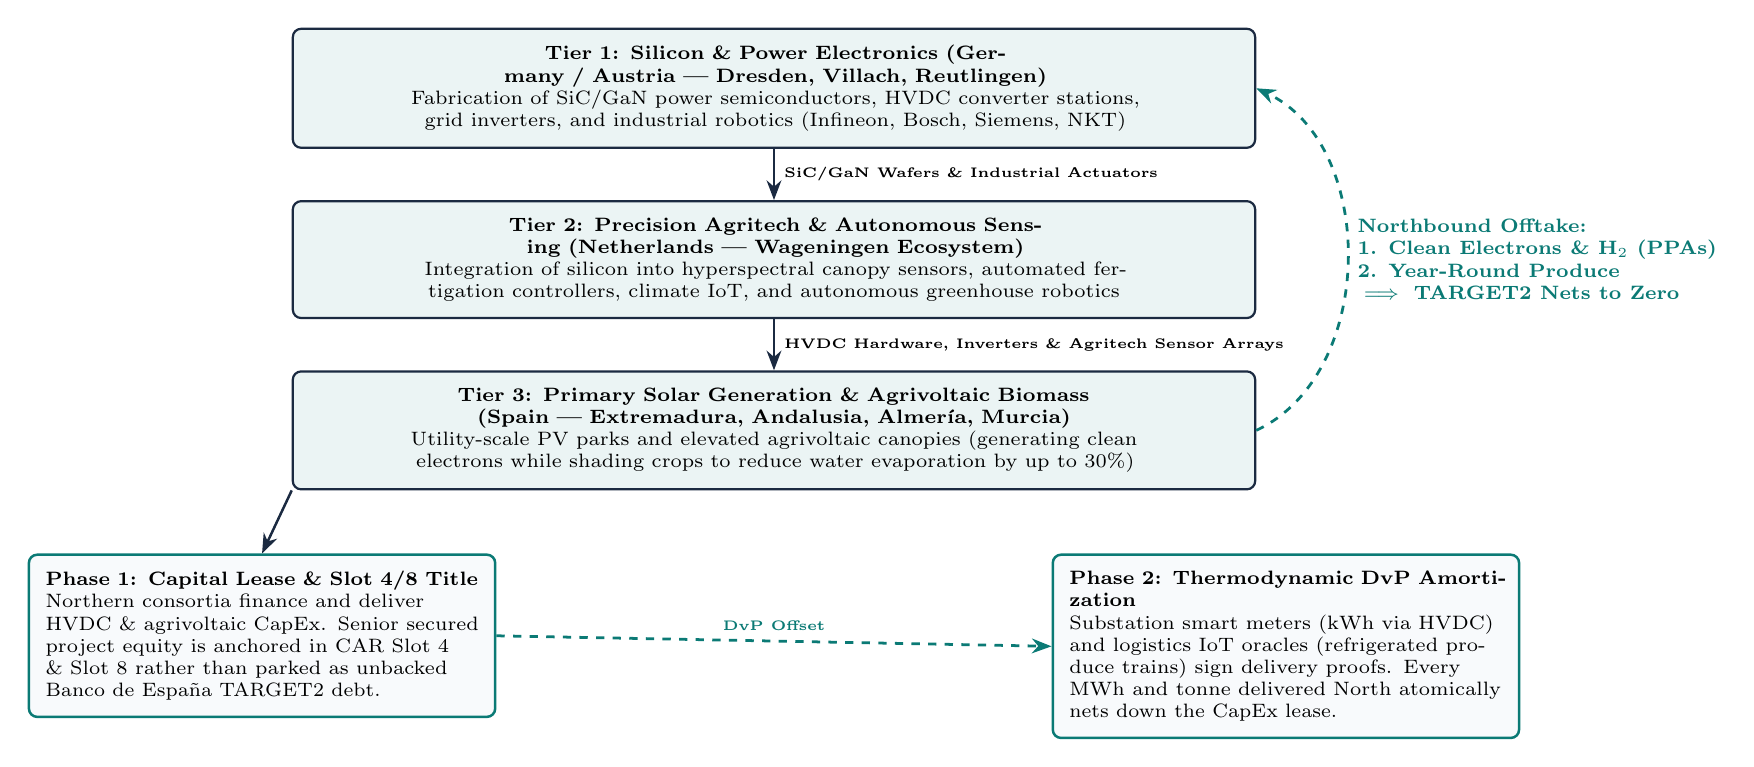
\begin{tikzpicture}[
  node distance=0.9cm and 1.4cm,
  tierbox/.style={draw=ink, fill=accent!8, rounded corners=3pt, line width=0.8pt, font=\scriptsize, align=center, inner sep=6pt, text width=11.8cm},
  phasebox/.style={draw=accent, fill=codebg, rounded corners=3pt, line width=0.9pt, font=\scriptsize, align=left, inner sep=6pt, text width=5.5cm},
  flowarrow/.style={-{Stealth[length=2.5mm]}, line width=0.9pt, draw=ink},
  dvparrow/.style={-{Stealth[length=2.5mm]}, line width=1.0pt, draw=accent, dashed}
]
  % Continental 3-Tier Industrial & Thermodynamic Division of Labor
  \node[tierbox] (t_north) {\textbf{Tier 1: Silicon \& Power Electronics (Germany / Austria — Dresden, Villach, Reutlingen)}\\Fabrication of SiC/GaN power semiconductors, HVDC converter stations, grid inverters, and industrial robotics (Infineon, Bosch, Siemens, NKT)};
  
  \node[tierbox, below=0.65cm of t_north] (t_mid) {\textbf{Tier 2: Precision Agritech \& Autonomous Sensing (Netherlands — Wageningen Ecosystem)}\\Integration of silicon into hyperspectral canopy sensors, automated fertigation controllers, climate IoT, and autonomous greenhouse robotics};
  
  \node[tierbox, below=0.65cm of t_mid] (t_south) {\textbf{Tier 3: Primary Solar Generation \& Agrivoltaic Biomass (Spain — Extremadura, Andalusia, Almer\'ia, Murcia)}\\Utility-scale PV parks and elevated agrivoltaic canopies (generating clean electrons while shading crops to reduce water evaporation by up to $30\%$)};

  \draw[flowarrow] (t_north) -- node[right, font=\tiny\bfseries] {SiC/GaN Wafers \& Industrial Actuators} (t_mid);
  \draw[flowarrow] (t_mid) -- node[right, font=\tiny\bfseries] {HVDC Hardware, Inverters \& Agritech Sensor Arrays} (t_south);

  % Two-Phase DvP Amortization Boxes below
  \node[phasebox, below left=0.8cm and -2.6cm of t_south] (p1) {\textbf{Phase 1: Capital Lease \& Slot 4/8 Title}\\Northern consortia finance and deliver HVDC \& agrivoltaic CapEx. Senior secured project equity is anchored in CAR Slot~4 \& Slot~8 rather than parked as unbacked Banco de Espa\~na TARGET2 debt.};

  \node[phasebox, below right=0.8cm and -2.6cm of t_south] (p2) {\textbf{Phase 2: Thermodynamic DvP Amortization}\\Substation smart meters (kWh via HVDC) and logistics IoT oracles (refrigerated produce trains) sign delivery proofs. Every MWh and tonne delivered North atomically nets down the CapEx lease.};

  \draw[flowarrow] (t_south.south west) -- (p1.north);
  \draw[dvparrow] (p1.east) -- node[above, font=\tiny\bfseries, text=accent] {DvP Offset} (p2.west);
  \draw[dvparrow] (t_south.east) to[out=25, in=-25] node[right, font=\scriptsize\bfseries, text=accent, align=left] {Northbound Offtake:\\1. Clean Electrons \& $\text{H}_2$ (PPAs)\\2. Year-Round Produce\\$\implies$ \textbf{TARGET2 Nets to Zero}} (t_north.east);
\end{tikzpicture}
\caption{The Continental Thermodynamic and Industrial Circuit: replacing uncollateralized TARGET2 central-bank imbalances with a self-liquidating capital lease across German/Austrian silicon and HVDC tooling, Dutch precision agritech, and Spanish solar and agrivoltaic production.}
\label{fig:thermodynamic_target2_loop}
\end{figure}

The thermodynamic clearing circuit operates across four deterministic phases:
\begin{enumerate}[nosep]
  \item \textbf{Synthetic Project Equity and Ring-Fenced CapEx (Phase 1):} Northern equipment financiers and industrial consortia supply the high-specification capital goods—HVDC converter stations, subsea/land interconnectors, SiC/GaN inverters, and Dutch greenhouse automation. Rather than booking an unbacked sovereign liability, the financing syndicate retains senior cryptographic title over the specific generation and agrivoltaic assets in CAR Slot~4 and Slot~8.
  \item \textbf{Long-Term Industrial Offtake Agreements (PPAs \& Produce Corridors):} Northern industrial consumers (chemical complexes in Ludwigshafen, electric-arc steelworks in Duisburg, automotive plants in Bavaria, and Northern European retail grocery distribution networks) enter long-term Power Purchase Agreements (PPAs), green hydrogen offtake contracts, and agricultural supply commitments indexed directly to the Southern installations.
  \item \textbf{DvP for Electrons and Biomass (Phase 2):} Energy and physical produce become programmable settlement units. Certified smart meters equipped with hardware Secure Elements at cross-border HVDC substations—alongside weight and temperature IoT telemetry on refrigerated rail corridors—emit signed cryptographic delivery vouchers (\cref{sec:usecase_microgrid}). Instead of wiring gross fiat euros across commercial banks, each verified megawatt-hour injected North and each shipment of produce acts as an \textbf{atomic debt-service credit}, deducting directly from the outstanding infrastructure lease in real time.
  \item \textbf{Structural TARGET2 Retirement and Full Equity Vesting:} Over the amortization schedule, southbound capital goods and northbound solar electrons and agricultural output cancel each other out through continuous multilateral netting:
  \begin{equation}
    \Delta\text{TARGET2}_{\text{net}} = \sum_{t} \text{CapEx}_{\text{South}}(t) - \sum_{t} \Bigl( p_{\text{kWh}} \cdot E_{\text{North}}(t) + p_{\text{agri}} \cdot Q_{\text{North}}(t) \Bigr) \longrightarrow 0
    \label{eq:target2_amortization}
  \end{equation}
  Once the initial capital expenditure is fully amortized via physical offtake, $100\%$ of the project equity vests unencumbered to the local Spanish operators.
\end{enumerate}

\paragraph{Disintegrating the ``Moral Hazard vs.\ Mercantilism'' Trope.}
For two decades, European political cohesion has been poisoned by two symmetrical falsehoods: the Northern narrative of a ``profligate South'' demanding permanent transfer-union bailouts, and the Southern narrative of Northern mercantilist wage suppression choking periphery growth. Both narratives are artifacts of an accounting system that hides reciprocal physical dependencies inside un-netted TARGET2 balances. When Spain's comparative advantages—solar irradiance, land, and agrivoltaic yield—are wired directly into firm offtake contracts that power German heavy industry and feed Northern cities, Spain no longer runs structural deficits, Germany no longer accumulates uncollectible central-bank IOUs, and the ledger mirrors the true division of labor of the European Single Market.


\subsection{The SLA-NFT Financing Model: Beyond the SaaS / RadWorks Trap}
\label{sec:sla_nft}

To free open-source ecosystems from philanthropic grant cycles, services are formalized
as \textbf{Dynamic SLA NFTs} (utilizing ERC-721/ERC-5484 capability tokens):
\begin{itemize}
  \item \textbf{Continuous Revenue Streaming:} Enterprise clients purchase SLA NFTs
representing 6-month or 1-year service tiers. Contract deposits stream continuously
to core maintainer addresses on every validated block.
  \item \textbf{Programmatic Friction and Entitlements:} Holding an active SLA NFT unlocks:
\begin{itemize}
\item Priority access to pre-build binaries compiled inside SGX enclaves.
\item Priority relay indexing and write access on private Radicle seed nodes.
\item Direct incident escalation channels governed by Decentralized Service Level
Agreements (DSLA).
\end{itemize}
  \item \textbf{Hardware Enforcement:} The SLA capability is pushed directly to the client's
hardware token (NFC charm or TICKEY badge). Tapping the badge authenticates the user
against private enterprise infrastructure via the SIWE-OIDC bridge.
\end{itemize}

\subsection{Headless Multi-Rail Payment Settlement}

Enterprise procurement departments never interact with crypto exchanges or manage gas slips:
\begin{enumerate}
  \item \textbf{Ingestion:} Clients pay through ordinary corporate rails: SEPA Instant wires,
corporate credit cards, USDC, or EURe.
  \item \textbf{Virtual IBAN Resolution:} Payments hit a virtual IBAN (vIBAN / deIBAN) bound
directly to the provider's W3C DID in Slot~0.
  \item \textbf{Regulated Conversion:} Licensed banking gateways (e.g., Monerium proxy or
Pontes DLT) lock fiat and mint Commercial Bank Money Tokens (CBMT) directly to the
smart account.
  \item \textbf{Ambient Gas Settlement:} Ambient relayers bundle the transaction, burning
fractional native gas in the background. The enterprise receives an on-chain receipt
and an automated, VAT-compliant electronic invoice.
\end{enumerate}

\subsection{Velocity Economics, the Fisher Equation, and Velotility}
\label{sec:fisher_velocity}

Monetary theory often treats velocity of circulation as a passive, uninteresting variable.
In Irving Fisher's Equation of Exchange~\cite{fisher1911purchasing}:
\begin{equation}
M \cdot V = P \cdot Y
  \label{eq:fisher}
\end{equation}
classical monetarists assumed velocity $V$ to be constant, asserting that the money
supply $M$ alone dictates prices. In modern industrial reality, velocity exhibits severe,
secular declines (\cref{fig:velocity_money}). When circulation velocity collapses,
pumping fiat liquidity fails to stimulate productive output.

\begin{figure}[H]
\centering
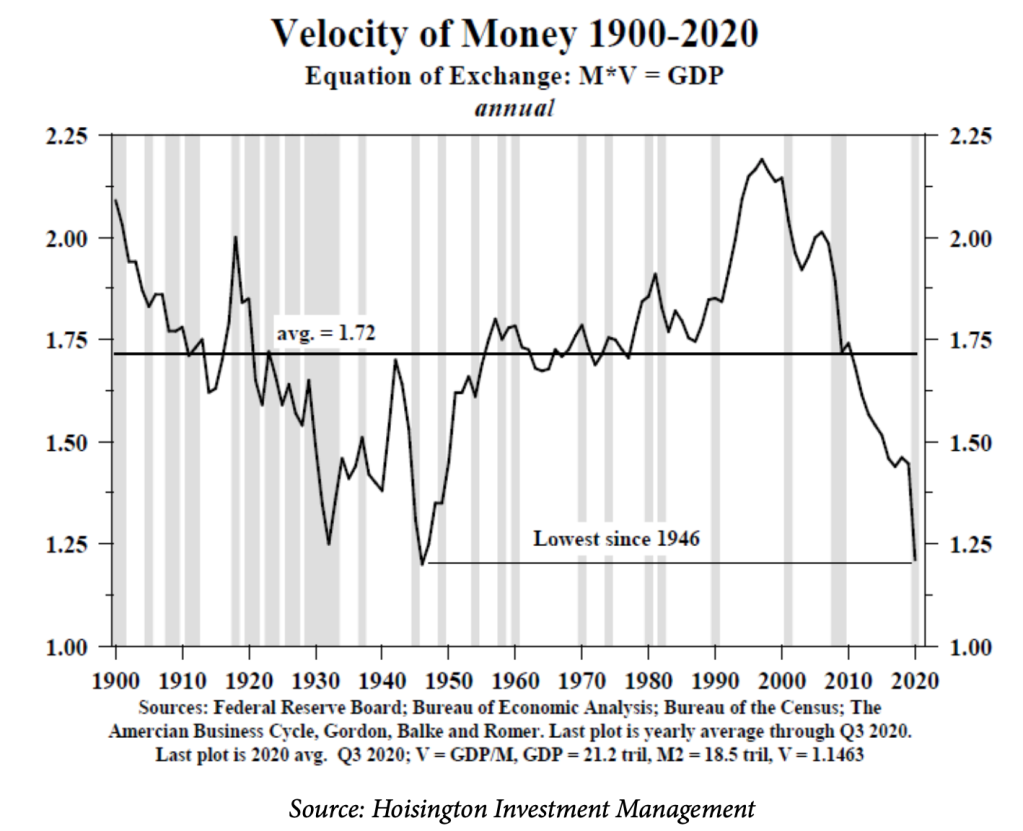
\includegraphics[width=0.96\linewidth]{img/velocity_of_money.png}
\caption{Empirical velocity of money trends (1900--2025), illustrating the secular collapse of fiat circulation velocity and the structural failure of raw monetary base expansion without real clearing velocity.}
\label{fig:velocity_money}
\end{figure}

In the Sovereign Bunny architecture, we reinterpret the classical Fisher Equation of Exchange ($MV = PQ$)~\cite{fisher1911} not as a static accounting identity, but as a dynamic control system where circulation velocity $V$ is the primary exogenous ``heartbeat'' dictating the ceiling of industrial output $Q$.
We reconcile MMT credit expansion with thermodynamic stability and neoclassical growth theory~\cite{solow1956,cobbdouglas1928} through \textbf{velotility} (\cref{fig:velotility_curve}):
\begin{equation}
Q(V) = k \cdot V^\alpha \cdot e^{-\delta V}
  \label{eq:velotility}
\end{equation}
Where $V$ represents verified transactional note velocity acting as circulating working capital, $k$ models baseline Total Factor Productivity (TFP)~\cite{solow1956}, $\alpha \in (0, 1)$ governs the Cobb--Douglas output elasticity of circulation velocity, and $\delta > 0$ imposes thermodynamic capital depreciation and dissipation against speculative churn. 

\begin{figure}[H]
\centering
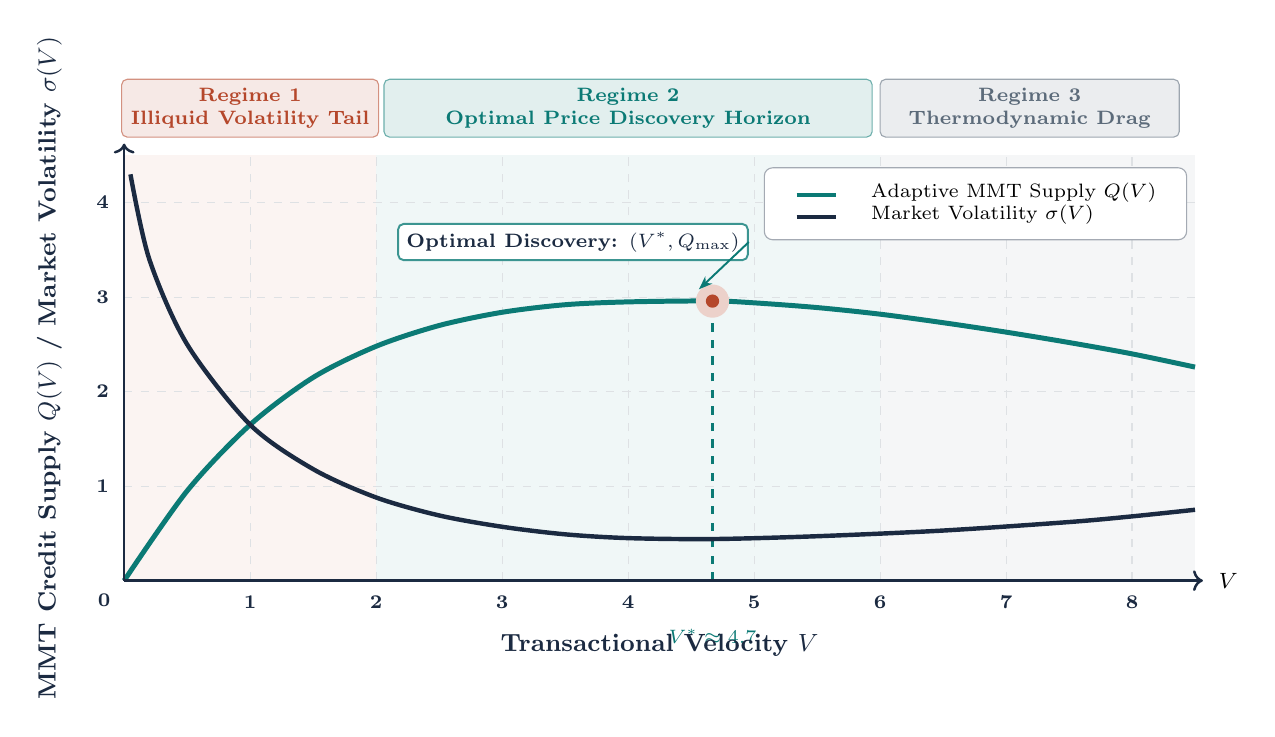
\begin{tikzpicture}[
  scale=1.0,
  every node/.style={font=\small},
  axis/.style={->, line width=0.9pt, draw=ink},
  gridline/.style={draw=mute!20, line width=0.4pt, dashed},
  volcurve/.style={draw=ink, line width=1.6pt},
  supplycurve/.style={draw=accent, line width=1.8pt}
]
  % Dedicated Top Header Banners (Generously spaced above the plot canvas)
  \node[draw=warn!60, fill=warn!12, rounded corners=2pt, font=\scriptsize\bfseries, text=warn, minimum width=3.0cm, minimum height=6.5mm, align=center] at (1.60, 6.0) {Regime 1\\Illiquid Volatility Tail};
  \node[draw=accent!60, fill=accent!12, rounded corners=2pt, font=\scriptsize\bfseries, text=accent, minimum width=6.2cm, minimum height=6.5mm, align=center] at (6.40, 6.0) {Regime 2\\Optimal Price Discovery Horizon};
  \node[draw=mute!60, fill=mute!12, rounded corners=2pt, font=\scriptsize\bfseries, text=mute, minimum width=3.8cm, minimum height=6.5mm, align=center] at (11.50, 6.0) {Regime 3\\Thermodynamic Drag};

  % Shaded Background Canvas Fills for Economic Regimes
  \fill[warn!6] (0, 0) rectangle (3.20, 5.4);
  \fill[accent!6] (3.20, 0) rectangle (9.60, 5.4);
  \fill[mute!6] (9.60, 0) rectangle (13.60, 5.4);

  % Full Internal Grid lines & X-Axis Ticks (dx = 1.60cm per unit)
  \foreach \x in {1,2,3,4,5,6,7,8} {
    \draw[gridline] (\x*1.60, 0) -- (\x*1.60, 5.4);
    \node[below=2pt, font=\scriptsize\bfseries, text=ink] at (\x*1.60, 0) {\x};
  }
  % Full Internal Grid lines & Y-Axis Ticks (dy = 1.20cm per unit)
  \foreach \y in {1,2,3,4} {
    \draw[gridline] (0, \y*1.20) -- (13.60, \y*1.20);
    \node[left=2pt, font=\scriptsize\bfseries, text=ink] at (0, \y*1.20) {\y};
  }
  \node[below left=2pt, font=\scriptsize\bfseries, text=ink] at (0, 0) {0};

  % Optimal Peak Guidance Line (V* = 4.67 -> x = 7.472, y = 3.55)
  \draw[draw=accent, line width=0.8pt, dashed] (7.472, 0) -- (7.472, 3.55);
  \node[below=14pt, font=\scriptsize\bfseries, text=accent] at (7.472, 0) {$V^* \approx 4.7$};

  % Adaptive MMT Money Supply Curve Q(V)
  \draw[supplycurve, smooth] plot coordinates {
    (0.0, 0.0)
    (0.5*1.60, 0.95*1.20)
    (1.0*1.60, 1.65*1.20)
    (1.5*1.60, 2.15*1.20)
    (2.0*1.60, 2.48*1.20)
    (2.5*1.60, 2.70*1.20)
    (3.0*1.60, 2.84*1.20)
    (3.5*1.60, 2.92*1.20)
    (4.0*1.60, 2.95*1.20)
    (4.67*1.60, 2.96*1.20)
    (5.0*1.60, 2.94*1.20)
    (5.5*1.60, 2.89*1.20)
    (6.0*1.60, 2.82*1.20)
    (6.5*1.60, 2.73*1.20)
    (7.0*1.60, 2.63*1.20)
    (7.5*1.60, 2.52*1.20)
    (8.0*1.60, 2.40*1.20)
    (8.5*1.60, 2.26*1.20)
  };

  % Asset Volatility Curve sigma(V)
  \draw[volcurve, smooth] plot coordinates {
    (0.05*1.60, 4.30*1.20)
    (0.20*1.60, 3.40*1.20)
    (0.50*1.60, 2.50*1.20)
    (1.00*1.60, 1.65*1.20)
    (1.50*1.60, 1.18*1.20)
    (2.00*1.60, 0.88*1.20)
    (2.50*1.60, 0.69*1.20)
    (3.00*1.60, 0.57*1.20)
    (3.50*1.60, 0.49*1.20)
    (4.00*1.60, 0.45*1.20)
    (4.67*1.60, 0.44*1.20)
    (5.50*1.60, 0.47*1.20)
    (6.50*1.60, 0.53*1.20)
    (7.50*1.60, 0.62*1.20)
    (8.00*1.60, 0.68*1.20)
    (8.50*1.60, 0.75*1.20)
  };

  % Optimum Marker Point & Halo
  \fill[warn!25] (7.472, 3.55) circle (6pt);
  \fill[warn] (7.472, 3.55) circle (2.4pt);

  % Callout Tag for Optimum Point (Positioned above-left of peak, with small pointer arrow)
  \node[fill=white, draw=accent!80, line width=0.7pt, rounded corners=2pt, font=\scriptsize\bfseries, text=ink, inner sep=3pt] (optTag) at (5.7, 4.3) {Optimal Discovery: $(V^*, Q_{\max})$};
  \draw[-{Stealth[scale=0.8]}, accent, line width=0.7pt] (optTag.east) -- (7.3, 3.7);

  % Axes
  \draw[axis] (0, 0) -- (13.7, 0) node[right=2pt, font=\footnotesize\bfseries] {$V$};
  \draw[axis] (0, 0) -- (0, 5.55);
  \node[below=16pt, font=\small\bfseries, text=ink] at (6.8, 0) {Transactional Velocity $V$};
  \node[rotate=90, anchor=center, font=\small\bfseries, text=ink] at (-0.95, 2.7) {MMT Credit Supply $Q(V)$ / Market Volatility $\sigma(V)$};

  % Dedicated Legend Box (Upper right quadrant in Regime 3, well clear of the peak)
  \node[draw=ink!40, fill=white, rounded corners=3pt, font=\scriptsize, anchor=north east, inner sep=5pt] at (13.5, 5.25) {
    \begin{tabular}{cl}
      \tikz\draw[supplycurve, line width=1.4pt] (0,0) -- (0.5, 0); & Adaptive MMT Supply $Q(V)$\\
      \tikz\draw[volcurve, line width=1.4pt] (0,0) -- (0.5, 0); & Market Volatility $\sigma(V)$\\
    \end{tabular}
  };
\end{tikzpicture}
\caption{The Velotility Curve: adaptive MMT credit supply expansion $Q(V)$ plotted across three economic regimes (illiquid tail, optimal price discovery horizon, and thermodynamic drag), rendered as a spacious, publication-grade vector chart.}
\label{fig:velotility_curve}
\end{figure}

The curve $Q(V)$ delineates three foundational economic regimes:
\begin{enumerate}
  \item \textbf{The Illiquidity and High-Volatility Tail ($V \to 0$):} Characterized by liquidity traps and extreme friction. With a low monetary base and depressed circulation velocity, assets are thin and illiquid. Price discovery fails, and potential coordination is lost to hoarding. Pumping unbacked fiat liquidity cannot resolve this trap because physical goods cannot clear without active velocity.
  \item \textbf{The Optimal Regime ($V \approx V^* = \alpha/\delta$):} The \textbf{``Switzerland Sweet Spot''}. At this peak, transaction velocity is perfectly synchronized with the industrial capacity of the network. The sheer volume of verified engineering output ``soaks up'' the money supply, establishing a benign, productivity-driven deflationary environment where the purchasing power of the currency appreciates due to surplus physical throughput.
  \item \textbf{The Overheated Regime ($V > V^*$):} When speculative velocity accelerates into high-frequency churn, recursive arbitrage loops, and wash trading, the thermodynamic decay term $e^{-\delta V}$ dominates. High velocity represents noise rather than productive signal, leading to entropic bubbles and systemic contraction.
\end{enumerate}

\subsubsection{Theoretical Foundations: From Solow to Minsky}
\label{sec:velotility_math}

To formally characterize the money supply elasticity curve $Q(V)$, we synthesize neoclassical growth theory~\cite{solow1956,cobbdouglas1928} with institutional transaction economics and financial instability:
\begin{enumerate}
  \item \textbf{Neoclassical Foundation and Productive Elasticity:} Drawing from Robert Solow~\cite{solow1956} and the Cobb--Douglas production function~\cite{cobbdouglas1928}, we define the relationship between circulation and coordination as one of diminishing marginal returns: $Q(V) = k V^\alpha$ ($0 < \alpha < 1$). Initial increases in $V$ facilitate the division of labor and reduce Coasean transaction costs~\cite{coase1937}. Here, $\alpha$ represents \textbf{Productive Elasticity}---the efficiency with which a cryptographic transaction (``handshake'') translates into verified real-world output (a manufactured ``brick'' or merged pull request).
  \item \textbf{Minsky's Financial Instability and Thermodynamic Drag:} To bridge growth theory with financial reality, we integrate Hyman Minsky's \textbf{Financial Instability Hypothesis}~\cite{minsky1992}. As the network nears capacity, stability breeds instability: high velocity decouples into speculative churn, recursive lending loops, and automated arbitrage that do not map to physical production. To model this transition from productive coordination to entropic friction, we introduce the saturation decay constant $\delta > 0$, yielding the Sovereign Output Function:
  \begin{equation}
    Q(V) = k \cdot V^\alpha \cdot e^{-\delta V}
  \end{equation}
  \item \textbf{The Velocity Golden Rule Analogy ($V = V^*$):} Differentiating $Q(V)$ with respect to $V$ and setting the derivative to zero:
  \begin{equation}
    \frac{dQ}{dV} = k e^{-\delta V} \left( \alpha V^{\alpha-1} - \delta V^\alpha \right) = 0 \iff \frac{\alpha}{V^*} - \delta = 0 \implies V^* = \frac{\alpha}{\delta}
    \label{eq:velotility_optimum}
  \end{equation}
  Equation~(\ref{eq:velotility_optimum}) reveals a formal equivalence to the \textbf{Solow--Phelps Golden Rule of Capital Accumulation}~\cite{solow1956,phelps1961}. In neoclassical growth, optimal consumption occurs where the marginal product of capital equals the depreciation rate ($f'(k^*) = \delta$). In velotility, optimal credit throughput occurs precisely when the marginal factor product of velocity ($\alpha / V$) balances the thermodynamic dissipation rate ($\delta$), yielding maximum throughput $Q_{\max} = k (\alpha/\delta)^\alpha e^{-\alpha}$.
\end{enumerate}

\paragraph{The Productivity-Inflation Nexus.}
The interaction between systemic throughput and monetary stability is governed by a quadratic inflation response $\pi(V)$ modeling the gap between money supply $M$ and adjusted output $Q(V)$:
\begin{equation}
  \pi(V) = a \left( M - \beta Q(V) \right) + b \left( M - \beta Q(V) \right)^2
  \label{eq:inflation_nexus}
\end{equation}
The model reveals a critical Stagnation Trap at depressed velocity ($V \to 0$): inflation spikes because too few physical goods are produced to absorb circulating liquidity. Conversely, in the overheated regime ($V > V^*$), output decays due to speculative noise, causing inflation to spike non-linearly. The ``Switzerland'' sweet spot occurs at the base of the curve, where $\pi$ is minimized because industrial output $Q$ is maximized.

\paragraph{Parameter Selection, Protocol Telemetry, and Velocity Decomposition.}
To guarantee that the network operates within the optimal corridor, the protocol monitors $\alpha$ and $\delta$ as live on-chain telemetry:
\begin{itemize}[nosep]
  \item \textbf{Elasticity ($\alpha = 0.7$):} Calibrated to ensure high coordination responsiveness while respecting the physical and cognitive throughput limits of the DAO's maintainers.
  \item \textbf{Decay Sensitivity ($\delta = 0.15$):} Calibrated to on-chain arbitrage frequency. Setting $\alpha = 0.7$ and $\delta = 0.15$ yields the optimal velocity peak $V^* = 0.7 / 0.15 \approx 4.67$, matching the empirical calibration plotted in \cref{fig:velotility_curve}.
  \item \textbf{Velocity Decomposition (Signal vs.\ Noise):} Total velocity is decomposed into productive and speculative components:
  \begin{equation}
    V = V_p + V_s
  \end{equation}
  Where $V_p$ represents productive transactions (wages, hardware leases, raw material procurement) verified via Heartbeat Oracles, and $V_s$ represents speculative trading. If $V_s \gg V_p$, the protocol detects an elasticity collapse ($a \to 0$), activating the Velocity Target Band policy to throttle high-frequency recursive loops and steer capital back toward the productive frontier.
\end{itemize}

\subsubsection{Issuance Circuit Breakers, Negative Elasticity, and Thermodynamic Drain}
\label{sec:circuit_breaker}

The protocol's emission function $I$ is not a static monetary constant but a dynamic derivative of verified industrial output $Q(V)$ and transactional velocity $V$~\cite{blum2024lightbook}. To prevent recursive financial leverage and restaking contagion, the Sovereign Stack implements an automated, evidence-based \textbf{Circuit Breaker}:
\begin{enumerate}[nosep]
  \item \textbf{The Efficiency Ratio and Zero-Issuance Threshold:} Protocol emission is modulated by the systemic efficiency ratio:
  \begin{equation}
    \eta = \frac{Q(V)}{V}
  \end{equation}
  When velocity accelerates without a corresponding increase in verified physical output ($Q$), the system classifies the activity as entropic noise ($V_s \gg V_p$). If $\eta$ drops below a statutory floor $\eta_{\min}$, new token issuance enters an immediate \textbf{Halt State} ($I = 0$). Maintainer and miner compensation shifts entirely to BASEFEE redirects and transaction fees, ensuring zero new supply enters an overheated, unproductive market.
  \item \textbf{Negative Elasticity (Thermodynamic Drain):} If real output $Q$ drops below a survival floor (e.g., severe supply-chain shocks or network partitions), the protocol activates contraction mode. The \textbf{Recycling Drain} accelerates: a dynamic \textbf{Social Slag Tax} is levied on high-velocity, low-output accounts, systematically burning supply to create a monetary vacuum that preserves purchasing power and averts currency debasement.
  \item \textbf{Programmatic Evidence-Based Halts:} Unlike legacy protocols reliant on manual multisig emergency pauses, the halt is deterministic:
  \begin{itemize}[nosep]
    \item \emph{Actuator Heartbeat Breaches:} If $>30\%$ of registered industrial actuators report an active DSLA breach or power disruption, issuance halts within a single block.
    \item \emph{Oracle Divergence:} If the internal valuation of the circulating unit deviates from the real-world raw materials index committed in Slot~4, the minting precompile freezes automatically.
  \end{itemize}
\end{enumerate}

\subsection{The On-Chain Banking Stack: deIBAN, deSWIFT, and Value-Packet Routing}
\label{sec:zkviban_kyc}

Traditional cross-border foreign exchange (FX) and interbank trade rely on correspondent banking networks connected by legacy SWIFT messaging. This imposes the \textbf{``SWIFT Tax''}: multi-day settlement delays ($T+2$), opaque intermediary markups, and predatory wire fees ($30$--$100$\,\EUR{} per transfer). The Sovereign Stack eliminates this friction through a decentralized banking stack that decouples identifiers from settlement infrastructure~\cite{blum2024lightbook,blum2024vision}.

\subsubsection{vIBAN and vSWIFT: Verifiable Financial Endpoints}

We extend Ethereum Name Service (ENS) records to host standardized, cryptographically verifiable financial routing endpoints:
\begin{itemize}[nosep]
  \item \textbf{vIBAN (Virtual IBAN):} An ENS text record (e.g., \code{viban=EE471000001020145685}) bound directly to the user's sovereign domain (\code{innovator.eth}). An associated \code{accepted} record defines supported currencies and settlement layers (e.g., \path{accepted=eth@taiko,usdc@base,eure@etc}).
  \item \textbf{Hierarchical Smart Contract Resolvers:} A two-tier on-chain resolver network routes payments deterministically:
  \begin{enumerate}[label=(\alph*),nosep]
    \item \emph{Country Resolver:} Parses the ISO country code (e.g., \code{EE}) and routes to the authorized national or consortium resolver.
    \item \emph{Bank Resolver:} Validates the Basic Bank Account Number (BBAN) and resolves the target smart account and ENS domain.
  \end{enumerate}
  \item \textbf{deIBAN Fallback to Burn Address:} If an IBAN query fails to resolve an equivalent vIBAN on-chain (returning a \code{NOROUTE} signal), the system routes to a verified redemption contract (e.g., Monerium-style burn address). Burning EURe triggers an automated off-chain SEPA credit via licensed proxy gateways, seamlessly bridging legacy accounts without exposing users to custodial risks.
  \item \textbf{vSWIFT and Value-Packet Routing (VPR):} International trade instructions are transmitted as \textbf{vSWIFT} packets across the high-speed rollup backbone. Unlike legacy SWIFT, where messages and settlement are divorced, vSWIFT bundles payment instructions atomically with zero-knowledge proofs of solvency. Capital flows as Standardized Financial Packets (SFPs) across a \emph{Double-Decker Stablecoin Sandwich} (e.g., instant Yuan $\leftrightarrow$ EURe swaps), achieving atomic finality in milliseconds.
  \item \textbf{Dual-Penalty System (Slag vs.\ Breach):} Liquidity providers (LPs) in the routing mesh are governed by protocol invariants:
  \begin{itemize}[nosep]
    \item \emph{Slag Penalty:} If an SFP exceeds its Time-to-Live (TTL) block height without settlement or explicit rejection, the LP incurs an automated State-Bloat Tax.
    \item \emph{Breach Slash:} If an LP locks a packet but fails to fulfill settlement before the TTL, the transaction triggers pull-based reclamation, and the LP's bonded collateral is slashed to pay the recipient a Latency Rebate.
  \end{itemize}
\end{itemize}

\subsubsection{zkvIBAN and Decentralized Dynamic KYC for CBMT Settlement}

Under statutory European and international banking regulations (including the EU Transfer of
Funds Regulation / Travel Rule and Basel Core Principles), Commercial Bank Money Tokens (CBMT)
are formal statutory liabilities of licensed commercial credit institutions. Consequently,
\textbf{the legal receiver or bearer of a CBMT must maintain an identified customer account at
a regulated commercial bank}.

To prevent this statutory mandate from degenerating into a centralized onboarding bottleneck,
the Sovereign Bunny architecture establishes a \textbf{decentralized KYC registry} anchored in
W3C and DIF Decentralized Identifiers (Slot~0)~\cite{dif2021did}:
\begin{enumerate}
  \item \textbf{On-the-Fly Commercial Bank Account Instantiation:} When an incoming payment hits
the provider's DID, a regulated bank partner uses the decentralized KYC registry to instantiate
a fully compliant virtual IBAN (\textbf{zkvIBAN}) on the fly. The receiver never fills out manual
PDF forms or waits weeks for compliance approval.
  \item \textbf{Risk-Adjusted Dynamic KYC Overlap:} Rather than relying on a single fallible KYC
provider, compliance credentials are cross-verified across an overlapping consortium of regulated
identity anchors (e.g., eIDAS qualified trust service providers, European national identity gateways,
and licensed banking partners). 
  \item \textbf{Dynamic Risk Tiering:} Low-value industrial micro-settlements require single-attestation
proofs, whereas high-volume cross-border treasury settlements require an overlapping quorum of
multiple independent KYC verifiers. Regulators receive mathematical certainty that all statutory
anti-money laundering (AML) requirements are fulfilled, while the customer's personal data remains
securely encrypted within their private DID document.
\end{enumerate}

\subsection{The SLA-NFT Engine: Collectible Season Passes and Post-SLA Tradability}
\label{sec:sla_nft_tradability}

In legacy Web2 enterprise SaaS, software licenses and service-level agreements (SLAs) are pure operational
sunk costs: when an annual license expires, the customer retains zero residual asset value.

In the Sovereign Bunny stack, enterprise software licensing is formalized as a \textbf{Dynamic SLA-NFT}:
\begin{enumerate}
  \item \textbf{Per-Seat and Operation-Wide Licensing:} When an enterprise licenses a software release,
micro-cluster deployment, or infrastructure service during an active billing season (e.g. quarterly or annual billing window),
each seat holder or operating unit is issued an on-chain NFT from a curated generative collection.
  \item \textbf{The ``Those Who Know'' Series Monster Archetype:} In our reference implementation, each licensed seat
receives a generative NFT featuring the ``Those Who Know'' monster series (\cref{fig:monster_badges}).
Generative AI models cross the base monster archetype with the licensee company's corporate identity, assigned permissions,
and sponsorship tier, producing a unique tactile badge.
  \item \textbf{The SLA-Locked Capability Invariant:} Throughout the active billing season, the NFT is non-transferable (soulbound).
It functions as a cryptographic capability token granting priority access to attested SGX nightly builds, Radicle Slot~3 repositories,
and seed nodes.
  \item \textbf{Secondary Tradability Upon SLA Expiration and Capability Isolation:} The exact instant the service-level agreement for that billing season
expires and maintenance accounts settle on-chain, \textbf{the NFT transforms into an unencumbered, freely tradable digital collectible}.
Employees, enthusiasts, and secondary collectors can trade, auction, or showcase these season passes on secondary markets,
converting historical corporate software expenditure into collectible digital heritage.
\textbf{Cryptographic Capability Isolation:} To prevent secondary collectors from exploiting expired tokens to masquerade as active enterprise seat-holders, the runtime precompiles governing Slot~1 (Zanzibar ReBAC) and Slot~3 (Radicle tag signing) enforce strict active epoch bounds $[E_{\text{start}}, E_{\text{end}}]$ on-chain. An expired NFT conveys immutable historical provenance, artwork ownership, and community prestige, but grants \textbf{precisely zero operational execution capability, SGX build access, or repository write permissions}.
\end{enumerate}

\subsection{zkTaxCompliance: Automated Tax Remittance and Zero-Knowledge Fiscal Audits}
\label{sec:zk_tax_compliance}

A persistent barrier to enterprise blockchain adoption is fiscal and tax compliance: conventional systems force companies
either to publicly disclose proprietary sales data on-chain, or maintain expensive, delayed manual accounting reconciliations.

In the Sovereign Bunny stack, statutory value-added tax (VAT) and corporate withholding tax are computed and remitted
\textbf{automatically inside the lattice state transition itself}:
\begin{equation}
  \text{Gross} = \text{Net} + \text{Tax}, \quad \text{Tax} = \left\lfloor \text{Net} \times \tau_{\text{rate}} \right\rfloor
\end{equation}
During the state transition, the payment is split atomically: the net obligation flows to the merchant's account,
while the tax fraction is routed directly to the designated municipal or federal tax authority's escrow vault on Eurosystem Pontes.

The merchant generates a succinct \textbf{zkTaxProof} asserting compliance without disclosing trade secrets:
\begin{enumerate}
  \item \textbf{Statutory Tax Rate Verification:} Proves that for all invoices committed in Slot~4 ($R_4$), the exact legal tax rate $\tau_{\text{rate}}$ (e.g. 19\% German MwSt) was remitted to the public treasury.
  \item \textbf{Zero Leaked Trade Secrets:} The proof conceals customer identities, line-item margins, wholesale supplier discounts, and individual sales volumes from the tax auditor.
  \item \textbf{Instant On-Chain Clearance:} The tax authority verifies the proof on-chain in $4$\,ms, automatically issuing an immutable, zero-knowledge tax clearance certificate.
\end{enumerate}

\Needspace{25\baselineskip}
\begin{lstlisting}[language=Noir,caption={Noir Circuit: Zero-Knowledge Value-Added Tax (VAT) Compliance Verifier (\code{circuits/src/zk\_tax\_compliance.nr})}]
use dep::std::merkle::compute_merkle_root;

fn main(
    // Public Inputs: Public tax authority vault, statutory tax rate (e.g. 1900 bps = 19%),
    // and total tax remitted to public treasury
    tax_authority_vault: pub Field,
    tax_rate_bps: pub u64,
    total_tax_remitted: pub u128,
    invoice_batch_merkle_root: pub Field,
    
    // Private Inputs: Itemized invoice details (hidden from tax inspector)
    net_amounts: [u128; 4],
    salts: [Field; 4],
    merkle_paths: [[Field; 4]; 4]
) {
    let mut accumulated_tax: u128 = 0;

    for i in 0..4 {
        // 1. Calculate statutory tax fraction for each confidential invoice:
        // Tax = floor(Net * tax_rate_bps / 10000)
        let invoice_tax: u128 = (net_amounts[i] * tax_rate_bps as u128) / 10000;
        accumulated_tax += invoice_tax;

        // 2. Verify invoice commitment in Slot 4 Proof of SQL Merkle tree
        let leaf_hash = std::hash::pedersen_hash([
            net_amounts[i] as Field,
            invoice_tax as Field,
            salts[i]
        ]);
        let derived_root = compute_merkle_root(leaf_hash, i as Field, merkle_paths[i]);
        assert(derived_root == invoice_batch_merkle_root);
    }

    // 3. Assert exact match with on-chain tax treasury remittance
    assert(accumulated_tax == total_tax_remitted);
}
\end{lstlisting}

\subsection{Vibe-Collateralized Bonds and the Tinyblock Token Distribution}

Traditional debt requires tangible real estate or cash reserves. The Sovereign Stack
formalizes human capital and developer momentum through \textbf{Vibe-Collateralized Bonds}
(utilizing ERC-3475 multi-compartment bonds) (\cref{fig:social_crypto_bonds}):
\begin{itemize}
  \item \textbf{Senior Tranche A:} Backed by tangible hardware nodes, edge blades, and inventory.
  \item \textbf{Junior Tranche D:} Backed by verified developer reputation and on-chain TinyMeritRank.
Margin calls are triggered exclusively by declines in verified engineering output.
\end{itemize}

\begin{figure}[H]
\centering
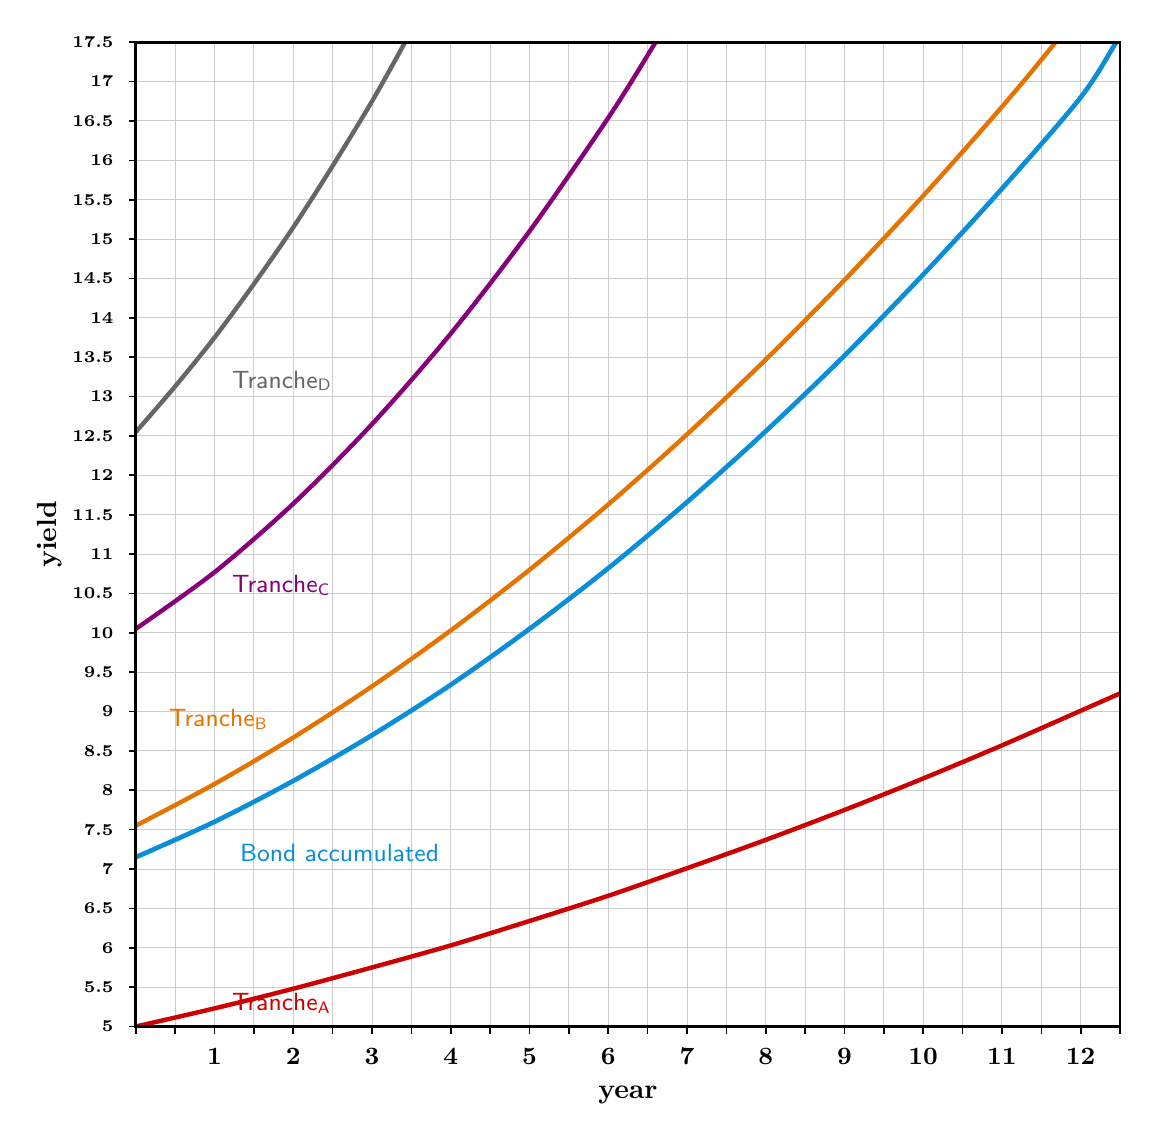
\begin{tikzpicture}[
  scale=1.0,
  every node/.style={font=\small},
  gridline/.style={draw=black!20, line width=0.35pt},
  trancheA/.style={draw=red!80!black, line width=1.6pt},
  trancheB/.style={draw=orange!90!black, line width=1.6pt},
  trancheC/.style={draw=purple!70!blue, line width=1.6pt},
  trancheD/.style={draw=black!60, line width=1.6pt},
  bondAcc/.style={draw=cyan!75!blue, line width=1.7pt}
]
  % Full Internal Grid lines (25 steps of 0.5 over 12.5cm x 12.5cm: dx = 0.50cm, dy = 0.50cm)
  \foreach \i in {1, 2, ..., 24} {
    \draw[gridline] (\i*0.50, 0) -- (\i*0.50, 12.50);
    \draw[gridline] (0, \i*0.50) -- (12.50, \i*0.50);
  }

  % Curves clipped strictly inside the 12.50cm x 12.50cm frame
  \begin{scope}
    \clip (0, 0) rectangle (12.50, 12.50);

    % Tranche D (Junior / First-Loss: reputation capital)
    \draw[trancheD, smooth] plot coordinates {
      (0.00, 7.55) (0.50, 8.13) (1.00, 8.75) (1.50, 9.43)
      (2.00, 10.15) (2.50, 10.93) (3.00, 11.75) (3.42, 12.50) (3.80, 13.20)
    };

    % Tranche C (Subordinated)
    \draw[trancheC, smooth] plot coordinates {
      (0.00, 5.05) (1.00, 5.77) (2.00, 6.64) (3.00, 7.65)
      (4.00, 8.80) (5.00, 10.10) (6.00, 11.54) (6.60, 12.50) (7.00, 13.20)
    };

    % Tranche B (Mezzanine: natural convex yield curve maintaining steady upward momentum)
    \draw[trancheB, smooth] plot coordinates {
      (0.00, 2.55) (1.00, 3.08) (2.00, 3.67) (3.00, 4.32)
      (4.00, 5.03) (5.00, 5.80) (6.00, 6.63) (7.00, 7.52)
      (8.00, 8.47) (9.00, 9.48) (10.00, 10.55) (11.00, 11.68)
      (11.68, 12.50) (12.20, 13.20)
    };

    % Bond accumulated (Blended Portfolio Yield)
    \draw[bondAcc, smooth] plot coordinates {
      (0.00, 2.15) (1.00, 2.60) (2.00, 3.12) (3.00, 3.70)
      (4.00, 4.34) (5.00, 5.05) (6.00, 5.82) (7.00, 6.66)
      (8.00, 7.56) (9.00, 8.52) (10.00, 9.55) (11.00, 10.64)
      (12.00, 11.80) (12.45, 12.50) (12.80, 13.10)
    };

    % Tranche A (Senior: physical collateral)
    \draw[trancheA, smooth] plot coordinates {
      (0.00, 0.00) (1.00, 0.23) (2.00, 0.48) (3.00, 0.75)
      (4.00, 1.03) (5.00, 1.34) (6.00, 1.66) (7.00, 2.01)
      (8.00, 2.37) (9.00, 2.75) (10.00, 3.15) (11.00, 3.57)
      (12.00, 4.01) (12.50, 4.23)
    };
  \end{scope}

  % Outer Enclosing Frame
  \draw[draw=black, line width=1.0pt] (0, 0) rectangle (12.50, 12.50);

  % Authentic On-Curve Typography (Exactly matching reference specification)
  \node[font=\small\sffamily, text=black!60, anchor=west] at (1.1, 8.2) {$\text{Tranche}_{\text{D}}$};
  \node[font=\small\sffamily, text=purple!70!blue, anchor=west] at (1.1, 5.6) {$\text{Tranche}_{\text{C}}$};
  \node[font=\small\sffamily, text=orange!90!black, anchor=west] at (0.3, 3.9) {$\text{Tranche}_{\text{B}}$};
  \node[font=\small\sffamily, text=cyan!75!blue, anchor=west] at (1.2, 2.2) {$\text{Bond accumulated}$};
  \node[font=\small\sffamily, text=red!80!black, anchor=west] at (1.1, 0.3) {$\text{Tranche}_{\text{A}}$};

  % X-Axis Ticks (every 0.5 step) & Labels (every whole integer year, 1 to 12)
  \foreach \i in {0, 1, ..., 25} {
    \draw[draw=black, line width=0.6pt] (\i*0.50, 0) -- (\i*0.50, -0.09);
  }
  \foreach \x in {1, 2, ..., 12} {
    \node[below=2pt, font=\small\bfseries, text=black] at (\x*1.0, -0.09) {\x};
  }
  \node[below=18pt, font=\normalsize\bfseries, text=black] at (6.25, 0) {year};

  % Y-Axis Ticks & Labels (Every single 0.5 yield step from 5 to 17.5)
  \foreach \i/\lbl in {
    0/{5}, 1/{5.5}, 2/{6}, 3/{6.5}, 4/{7}, 5/{7.5}, 6/{8}, 7/{8.5}, 8/{9}, 9/{9.5},
    10/{10}, 11/{10.5}, 12/{11}, 13/{11.5}, 14/{12}, 15/{12.5}, 16/{13}, 17/{13.5},
    18/{14}, 19/{14.5}, 20/{15}, 21/{15.5}, 22/{16}, 23/{16.5}, 24/{17}, 25/{17.5}
  } {
    \draw[draw=black, line width=0.6pt] (0, \i*0.50) -- (-0.09, \i*0.50);
    \node[left=2pt, font=\fontsize{6.5pt}{7.5pt}\selectfont\bfseries, text=black] at (-0.09, \i*0.50) {\lbl};
  }
  \node[rotate=90, anchor=center, font=\normalsize\bfseries, text=black] at (-1.10, 6.25) {yield};
\end{tikzpicture}
\caption{Vibe-Collateralized Multi-Compartment Bond architecture: empirical yield curves across senior physical tranches ($\text{Tranche}_{\text{A}}$), blended portfolio debt, and junior reputation tranches ($\text{Tranche}_{\text{D}}$), rendered with complete enclosing bounds, 25$\times$25 coordinate grids, and authentic on-curve labels.}
\label{fig:social_crypto_bonds}
\end{figure}

\subsubsection{Solidity Reference: ERC-3475 Vibe-Collateralized Multi-Compartment Bond}

The following Solidity contract enforces the multi-compartment structure of
Vibe-Collateralized Bonds, separating physical collateral (Tranche A) from
TinyMeritRank reputation collateral (Tranche D):

\Needspace{25\baselineskip}
\begin{lstlisting}[language=Solidity,caption={Solidity Implementation: ERC-3475 Vibe-Collateralized Bond (\code{contracts/src/VibeBondERC3475.sol})}]
// SPDX-License-Identifier: Apache-2.0
pragma solidity ^0.8.24;

interface ITinyMeritOracle {
    function getMeritRank(address entity) external view returns (uint256 scoreBps);
}

contract VibeBondERC3475 {
    struct Tranche {
        uint256 physicalCollateral; // Senior Tranche A
        uint256 reputationScore;    // Junior Tranche D
        uint256 minMeritScore;
        uint256 principalOwed;
        bool isDefaulted;
    }

    mapping(uint256 => Tranche) public tranches;
    ITinyMeritOracle public immutable meritOracle;

    event MarginCall(uint256 indexed trancheId, uint256 currentScore);
    event Liquidated(uint256 indexed trancheId, uint256 recoveredAmount);

    constructor(address _meritOracle) {
        meritOracle = ITinyMeritOracle(_meritOracle);
    }

    function checkSolvency(uint256 trancheId, address borrower) external {
        Tranche storage t = tranches[trancheId];
        require(!t.isDefaulted, "Already liquidated");

        uint256 currentScore = meritOracle.getMeritRank(borrower);

        // Reputation-Based Margin Call Threshold
        if (currentScore < t.minMeritScore) {
            emit MarginCall(trancheId, currentScore);
            
            // If reputation collapses below 50% of threshold, liquidate Senior physical collateral
            if (currentScore < t.minMeritScore / 2) {
                t.isDefaulted = true;
                emit Liquidated(trancheId, t.physicalCollateral);
            }
        }
    }
}
\end{lstlisting}

\subsubsection{The \$TINY Token Distribution and Sociostasis}

The reference Tinyblock network implements an anti-speculative monetary structure:
\begin{enumerate}
  \item \textbf{Supply Cap:} 1,000,000,000 \$TINY (fixed during Phase~1 Sociostasis). Zero DEX liquidity; zero VC rounds.
  \item \textbf{Constitutional Allocation:}
25\% Community Merit Epochs (TinyMeritRank);
25\% Protocol Treasury;
20\% Core Maintainers (8-year backloaded vesting);
20\% Ecosystem Bootstrap (hardware nodes);
10\% Protocol Insurance Reserve.
  \item \textbf{Eurovision-Style Federated Voting:} In the reference deployment, seven Regional DAOs (Europe, North America,
South America, Africa, Central Asia, East Asia, Oceania) evaluate each other's
verified physical infrastructure milestones annually, awarding protocol treasury
splits through a federated, non-self-voting matrix. The number seven is a deployment
parameter, not a protocol constant: the matrix is generic over its peer set $R$, and a region is simply a
DAO subgraph (\cref{sec:relationship_authority}).
\end{enumerate}

\subsubsection{Regional DAO Federated Voting Matrix Protocol}

To evaluate annual infrastructure progress across the 7 geographic regions without
self-dealing, the consensus engine runs the following non-self-voting tally algorithm:

\Needspace{25\baselineskip}
\begin{lstlisting}[language=Rust,caption={Rust Implementation: Federated Regional DAO Voting Matrix (\code{crates/consensus/src/federated\_voting.rs})}]
pub struct RegionalVotingMatrix<const R: usize> {
    pub ballots: [[u32; R]; R], // ballots[voter_region][candidate_region]
}

impl<const R: usize> RegionalVotingMatrix<R> {
    pub fn tally_protocol_shares(&self) -> Result<[f64; R], &'static str> {
        let mut total_scores = [0u64; R];
        
        for voter in 0..R {
            // Constitutional Rule: Regional DAOs cannot vote for themselves
            if self.ballots[voter][voter] != 0 {
                return Err("CONSTITUTIONAL VIOLATION: Self-voting strictly prohibited");
            }
            for candidate in 0..R {
                total_scores[candidate] += self.ballots[voter][candidate] as u64;
            }
        }

        let grand_total: u64 = total_scores.iter().sum();
        if grand_total == 0 {
            return Err("Zero ballots cast in evaluation round");
        }

        let mut shares = [0.0f64; R];
        for i in 0..R {
            shares[i] = total_scores[i] as f64 / grand_total as f64;
        }
        Ok(shares)
    }
}
\end{lstlisting}

\subsection{Storage as an Endowment}
\label{sec:storage}

Storage hosts are compensated only upon answering unpredictable retrievability challenges.
Accounting for media density declines against fixed datacenter power and cooling floors,
we bound the effective discount rate:
\begin{equation}
d_{\text{eff}} = \max\bigl(0,\, d_{\text{storage}} - \pi_{\text{energy}}\bigr)
\end{equation}
The perpetual endowment required to fund indefinite data retention is:
\begin{equation}
E = \sum_{t=0}^{\infty} c_0 (1 - d_{\text{eff}})^t = \frac{c_0}{d_{\text{eff}}}
\end{equation}
Unspent capital is preserved in a conservative protocol reserve, insulating decentralized
storage from energy price spikes~\cite{williams2019arweave}.

\subsection{Multilateral Netting across Heterogeneous Ledgers: Bridge-Free Consensus Clearing}
\label{sec:cross_ledger_netting}

A structural vulnerability of multi-chain ecosystems has been the reliance on centralized cross-chain bridges: multi-signature custodial contracts that lock assets on Chain~A and mint wrapped representations on Chain~B. Between 2021 and 2025, bridge exploits accounted for over \$2.8~billion in lost collateral.

The Sovereign Bunny architecture eliminates bridges entirely. By treating accounts as autonomous actors communicating via point-to-point Iroh QUIC streams and Blind Notes~\cite{williamson2022aztec}, \textbf{cross-ledger clearing occurs through mathematical multilateral netting}:
\begin{enumerate}
  \item \textbf{Decentralized Obligation Graph:} Commercial counterparties operating across disparate systems (e.g., enterprise SAP on AWS, a local Sovereign Bunny manifold, and legacy Ethereum mainnet) exchange encrypted debt commitments ($\Delta_{ij}$) as Blind Notes in Slot~2.
  \item \textbf{Decentralized Cycle Discovery via Local JEPA \& Blinded Probes:} Traditional multilateral netting historically required a centralized clearing house or heavy secure multi-party computation (SMPC) to reconstruct the global liability graph. The Sovereign architecture decentralizes cycle discovery without exposing private debt amounts:
  \begin{itemize}
    \item \textbf{Local JEPA Flow Embeddings:} Each node's local Joint-Embedding Predictive Architecture (JEPA) models liquidity flow vectors in continuous representation space ($\mathbb{R}^{256}$), predicting high-likelihood netting trajectories based on historical settlement cadences without decrypting counterparty data.
    \item \textbf{Blinded Probe Notes:} Autonomous agents dispatch ephemeral, blinded probe notes across Iroh QUIC channels. If a probe returns to its origin along a closed directed path, the cyclic closure $\mathcal{C}$ is proven without revealing intermediate balances.
    \item \textbf{Stateless Atomic Cancellation:} Once $\mathcal{C}$ is discovered, the cycle participants assemble a composite zero-knowledge clearing proof $\pi_{\text{clearing}}$, nullifying the gross liabilities in Slot~2 and settling the net reduction in a single atomic epoch.
  \end{itemize}
  \item \textbf{Bridge-Free Cyclic Netting:} The netting algorithm identifies closed debt cycles:
  \begin{equation}
    \mathcal{C} = \{(1 \to 2), (2 \to 3), \dots, (k \to 1)\}, \quad \Delta_{\text{net}} = \min_{(i,j) \in \mathcal{C}} \Delta_{ij}
  \end{equation}
  By subtracting $\Delta_{\text{net}}$ around the cycle, $70$--$85\%$ of gross liabilities cancel out mathematically. No tokens move between chains; no custodial lockboxes are created.
  \item \textbf{Residual Settlement via Eurosystem Pontes:} Only the non-cyclical residual net imbalance ($15$--$30\%$) requires physical settlement. This residual is submitted directly as a zero-knowledge proof $\pi_{\text{clearing}}$ to the Eurosystem Pontes endpoint~\cite{ecbpontes}, triggering automated central bank money (CeBM) settlement in TARGET2 or commercial bank deposit minting (CBMT).
\end{enumerate}

\subsection{The zkvIBAN Protocol: Zero-Knowledge Reverse-Resolution and Commercial Bank Money Tokens (CBMT)}
\label{sec:zkviban_protocol}

In legacy financial networks, the International Bank Account Number (IBAN) is a global public identifier permanently tied to a user's real-world identity in centralized bank core databases. Any public exposure of an IBAN allows bad actors to probe transaction histories, execute fraudulent direct debits, or conduct corporate surveillance.

\paragraph{What is a $\pi_{\text{vIBAN}}$?}
In the Sovereign Bunny architecture, a \textbf{$\pi_{\text{vIBAN}}$} is a stateless zero-knowledge reverse-resolution proof. In legacy retail and corporate banking, an IBAN routes to an identified account ledger in a centralized core banking database (such as SAP Banking or Finacle). In contrast, the Sovereign account-lattice stores \textbf{zero} on-chain mapping tables linking public addresses to fiat banking identifiers. Instead, banking interoperability is achieved via client-side cryptographic reverse-resolution:
\begin{enumerate}
  \item \textbf{Bank Consortium Merkle Root ($\mathcal{R}_{\text{vIBAN}}$):} A regulated alliance of participating commercial banks (e.g., regional German Sparkassen and Volksbanken under the DK framework~\cite{dk2023cbmt}) publishes and continuously updates an on-chain Sparse Merkle Tree root $\mathcal{R}_{\text{vIBAN}}$ containing authorized routing prefix allocations, licensed institution public keys, and cryptographic customer identity commitments.
  \item \textbf{Deterministic Local Derivation:} An account owner derives their virtual IBAN (\code{vIBAN}) locally from their Slot~0 ($R_0$) master seed:
  \begin{equation}
    \text{vIBAN} = \operatorname{KDF}(\text{Seed}_{\text{Slot0}}, \text{BankPrefix}, \text{AccountNonce})
  \end{equation}
  \item \textbf{Stateless Reverse-Resolution Proof ($\pi_{\text{vIBAN}}$):} When receiving an inbound SEPA Instant wire, a TARGET2 wholesale clearing credit, or a Commercial Bank Money Token (CBMT) transfer, the recipient's wallet executes a specialized client-side Noir circuit generating $\pi_{\text{vIBAN}}$:
  \begin{itemize}
    \item \textbf{Membership Assertion:} Proves that the claimed \code{vIBAN} is an authentic member of the banking consortium's committed root $\mathcal{R}_{\text{vIBAN}}$ without disclosing which specific branch or leaf index holds it.
    \item \textbf{Identity Binding:} Proves that the recipient's on-chain W3C DID and QSCD public key committed in Slot~0 ($R_0$) match the authorized private holder of that \code{vIBAN}:
    \begin{equation}
      \operatorname{Poseidon}(\text{vIBAN}, \text{salt}_{\text{bank}}, \text{privkey}_{\text{Slot0}}) = H_{\text{Slot0}}
    \end{equation}
    \item \textbf{Zero-Knowledge KYC/AML Compliance:} Proves that the account satisfies statutory European anti-money laundering thresholds (e.g., Tier~1 micro-payments below €1,000, Tier~2 corporate invoicing, or Tier~3 wholesale treasury) without disclosing the user's legal name, tax identification number, passport data, or residential address.
  \end{itemize}
  \item \textbf{Instant Consortium Crediting:} The bank gateway verifies $\pi_{\text{vIBAN}}$ in sub-10ms and credits funds directly into the user's sovereign account as native CBMT or EURe. The public ledger never records an address-to-IBAN phonebook, completely neutralizing surveillance while preserving strict regulatory auditability.
\end{enumerate}

\subsection{Two-Tier Settlement: German CBMT, PBOC e-CNY Architecture, and Eurosystem Pontes}
\label{sec:cbmt_pontes_comparison}

The sovereign ledger never touches central bank reserves directly. Tier~1 commercial
banks operate supervised gateways, verifying zero-knowledge clearing proofs
$\pi_{\text{clearing}}$ and endogenously minting \textbf{Commercial Bank Money Tokens (CBMT)}~\cite{dk2023cbmt}.
Interbank net claims settle in wholesale central bank money (CeBM) via the Eurosystem's Pontes
bridge into TARGET2 / TIPS (\cref{fig:tiers}, \cref{fig:pontes_cbmt_minting})~\cite{ecbpontes}.

\paragraph{Institutional Foundations: The German DK CBMT Framework.}
In 2023, \emph{Die Deutsche Kreditwirtschaft} (DK, the German Banking Industry Committee representing private banks, savings banks, and cooperative credit unions) published the foundational specification for the Commercial Bank Money Token (\textbf{CBMT})~\cite{dk2023cbmt}. The DK demonstrated that Industry 4.0 manufacturing, automated supply chains, and machine-to-machine micro-payments require programmable bank deposits on DLT. Crucially, a CBMT is not an unbacked algorithmic stablecoin or an e-money token issued by a non-bank intermediary; it is a direct legal liability on a licensed commercial bank's balance sheet, fully covered by statutory deposit insurance (EDIS, up to €100,000 per depositor) and eligible for central bank refinancing.

\paragraph{Global Parallels: PBOC Two-Tier e-CNY and Project mBridge.}
This two-tier institutional architecture mirrors the global state of the art in central bank digital currency engineering:
\begin{itemize}
  \item \textbf{The PBOC Two-Tier Model:} As formulated by the People's Bank of China (PBOC) Digital Currency Research Institute~\cite{pboc2021ecny}, the digital yuan (\emph{e-CNY}) operates strictly on a two-tier framework: the PBOC (Tier~0) issues wholesale digital currency to commercial banks, while commercial banks (Tier~1) distribute digital cash and manage retail wallets, KYC/AML compliance, and credit allocation. This prevents disintermediation of commercial banks and preserves the banking system's capacity for endogenous money creation.
  \item \textbf{Project mBridge Wholesale Settlement:} On the multilateral level, the Bank for International Settlements (BIS) Innovation Hub and the Project mBridge consortium (connecting the PBOC, HKMA, Bank of Thailand, and CBUAE) demonstrated that cross-border wholesale settlement achieves sub-second finality by allowing commercial banks to settle bilateral claims in central bank money across a shared DLT mesh~\cite{bis2024mbridge}, eliminating high-cost correspondent banking hierarchies.
\end{itemize}
The Sovereign Bunny stack synthesizes these models: Sovereign Reth operates at Tier~2 (operational ERP, mutual credit, and single-writer account-lattices), settling net residuals into Tier~1 commercial bank CBMTs, which in turn clear interbank imbalances in Tier~0 central bank money via the Eurosystem's Pontes trigger into TARGET2.

\begin{figure}[H]
\centering
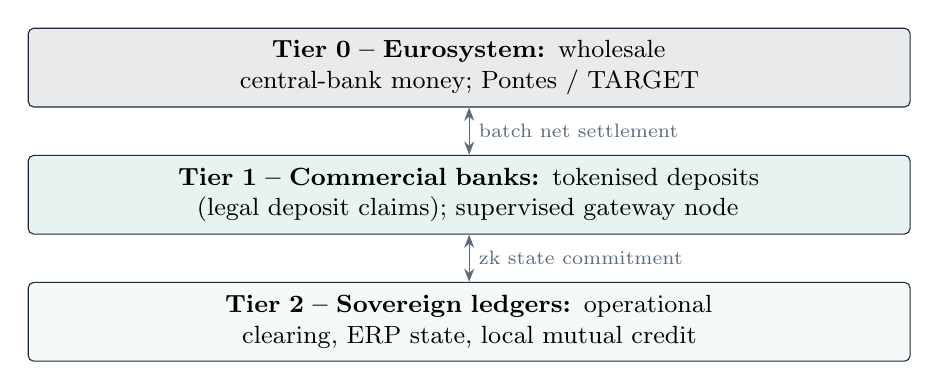
\begin{tikzpicture}[
  tier/.style={draw=ink,rounded corners=2pt,minimum width=11.2cm,text width=10.6cm,minimum height=10mm,
               align=center,font=\small},
  node distance=6mm]
  \node[tier,fill=ink!10] (t0) {\textbf{Tier 0 -- Eurosystem:} wholesale central-bank money; Pontes / TARGET};
  \node[tier,fill=accent!10,below=of t0] (t1) {\textbf{Tier 1 -- Commercial banks:} tokenised deposits (legal deposit claims); supervised gateway node};
  \node[tier,fill=accent!4,below=of t1] (t2) {\textbf{Tier 2 -- Sovereign ledgers:} operational clearing, ERP state, local mutual credit};
  \draw[{Stealth}-{Stealth},color=mute] (t0) -- (t1) node[midway,right,font=\scriptsize]{batch net settlement};
  \draw[{Stealth}-{Stealth},color=mute] (t1) -- (t2) node[midway,right,font=\scriptsize]{zk state commitment};
\end{tikzpicture}
\caption{Two-tier monetary hierarchy. The sovereign ledger never touches central-bank accounts directly.}
\label{fig:tiers}
\end{figure}

\begin{figure}[H]
\centering
\begin{tcolorbox}[colback=accent!4,colframe=accent,width=0.92\linewidth,arc=2pt,title={\small Endogenous CBMT Minting via Eurosystem Pontes}]
\centering\footnotesize\color{ink}
\begin{tabularx}{\linewidth}{|>{\raggedright\arraybackslash}X|>{\centering\arraybackslash}p{4.0cm}|>{\raggedright\arraybackslash}X|}
\hline
\textbf{Sovereign Ledger (Tier 2)} & $\longrightarrow$ \textbf{Bank Gateway (Tier 1)} $\longrightarrow$ & \textbf{Eurosystem (Tier 0)}\\
\hline
Slot 2 (Net Notes) / Slot 4 (SQL) & Noir / Proof of SQL Verifier & Pontes Infrastructure\\
$\pi_{\text{clearing}}$ state transition & Mints CBMT Credit Tokens & TARGET2 Trigger / TIPS DvP\\
Zero Plaintext Disclosed & Day-to-Day Operational Liquidity & CeBM Interbank Settlement\\
\hline
\end{tabularx}\\[4pt]
\emph{Commercial banks exercise statutory credit creation directly against mathematically verified proofs.}
\end{tcolorbox}
\caption{Cryptographic proof verification and endogenous CBMT minting via Eurosystem Pontes.}
\label{fig:pontes_cbmt_minting}
\end{figure}

\subsection{Regulatory Architecture under MiCA: Capital Discipline, Substance over Form, and the Demise of Offshore Arbitrage}
\label{sec:mica_regulatory_architecture}

The European Union's \textbf{Markets in Crypto-Assets Regulation (MiCA, Regulation EU 2023/1114)}~\cite{mica2023} represents a watershed moment for decentralized infrastructure. While superficial commentary in speculative crypto circles often decries European regulation as excessively stringent or bureaucratic, a rigorous legal and economic analysis reveals that MiCA provides the \textbf{clearest, cleanest, and most predictable regulatory operating environment in the world}. Unlike the United States—which has suffered through a decade of capricious ``regulation-by-enforcement,'' jurisdictional turf wars between the SEC and CFTC, and arbitrary court litigations—MiCA provides deterministic, codified statutory guardrails. Teams operating within European legal boundaries know with mathematical precision where they stand, creating the ideal institutional laboratory for deploying real-world cryptographic systems.

\subsubsection{The €1,000,000 Rolling Rule: Structural Capital Efficiency}
Under Article~4(2)(a) and Article~1(4)(c) of MiCA, crypto-asset offerings are explicitly exempt from the requirement to draft, notify, and publish an approved crypto-asset white paper if the total consideration of the offer in the Union does not exceed \textbf{€1,000,000 aggregated over a 12-month rolling window}~\cite{mica2023}.

This statutory ceiling is not an impediment; it is a vital mechanism of \textbf{post-ZIRP capital discipline}:
\begin{enumerate}
  \item \textbf{Eradication of Speculative Bloat:} During the 2017--2022 ZIRP bubble, protocol teams routinely raised \$20--50~million in speculative seed rounds before writing a single line of working code, creating bloated foundational overheads, misaligned venture capital incentives, and guaranteed token dumping on retail participants.
  \item \textbf{Lean Engineering and Rapid Product Validation:} The €1M exemption forces engineering teams to be hyper-efficient. It requires protocols to build functioning, working reference implementations, deploy autonomous physical hardware (such as mechanical Gachapon nodes), and establish endogenous customer revenue before seeking institutional capital.
  \item \textbf{Post-€1M Institutional Pathways:} Even when expanding beyond the €1M threshold, MiCA's statutory pathways remain remarkably liberal and pragmatic:
  \begin{itemize}
    \item \textbf{Qualified Investors Exemption (Article~4(2)(b)):} Projects can raise unlimited capital from accredited, professional, and institutional investors without producing a retail white paper.
    \item \textbf{NCA Notification Without Discretionary Merit Review (Article~8):} For public offerings above €1M, issuers must notify their National Competent Authority (NCA, such as BaFin in Germany or the AMF in France) at least 20 working days prior to publication. Crucially, under MiCA Article~8, \textbf{the NCA does not conduct a subjective ``merit review'' or issue a paternalistic business-model opinion}. The regulator's statutory duty is strictly to verify formal completeness, ensure transparency, and protect consumer disclosures. As long as the technical specifications, risk factors, and accounting invariants are truthfully disclosed, the offering proceeds.
  \end{itemize}
\end{enumerate}

\subsubsection{Consumer Protection and Incentive Alignment: Statutory Quality Regimes}
This regulatory focus on consumer protection and disclosure accuracy connects directly to the socio-technical dynamics observed in European statutory quality and production frameworks (\cref{sec:statutory_compliance}). Under the statutory framework for cooperative non-profit production and dispensing collectives:
\begin{itemize}
  \item Commercial speculative advertising and predatory retail markups are strictly banned.
  \item Operations must function on a transparent, cost-covering, cooperative mutual basis.
  \item Rigorous batch logging and verified testing standards protect consumers from adulteration.
\end{itemize}
MiCA enforces precisely the same economic alignment for cryptographic infrastructure: by removing deceptive speculative claims, mandating rigorous operational disclosures, and holding issuers legally accountable for misstatements, European law aligns developer incentives around authentic utility, solvency, and real-world industrial clearing rather than tokenized financial alchemy.

\subsubsection{Decentralization and the Doctrine of ``Substance over Form''}
A foundational pillar of European administrative law is the doctrine of \textbf{Substance over Form} (\emph{Substanz vor Form}): regulatory authorities evaluate the actual economic, technical, and operational reality of a system, rather than the nominal corporate wrappers or marketing slogans in which it is dressed.

MiCA codifies this doctrine in \textbf{Recital~22 and Article~2(2)}~\cite{mica2023}:
\begin{quote}
\emph{``Where crypto-asset services are provided in a fully decentralised manner without any intermediary, they should not fall within the scope of this Regulation.''}
\end{quote}
However, the doctrine of substance over form cuts both ways, radically altering the global competitive landscape:
\begin{itemize}
  \item \textbf{The Demise of Offshore Foundation Arbitrage (Switzerland and the Caymans):} For a decade, crypto projects established nominal non-profit foundations in Zug, Switzerland (\emph{Stiftungen}) or Cayman Islands / BVI SPVs, pretending they were ``decentralized DAOs'' while maintaining centralized GitHub push access, closed multisig treasuries, and coordinated market-making contracts. Under MiCA's strict reverse solicitation rules (\textbf{Article~61}), third-country offshore entities are barred from marketing or providing crypto services to EU residents without an authorized EU subsidiary. Because regulators look at substance, nominal offshore foundations with centralized keyholders are classified as unauthorized intermediaries, exposing their directors to direct administrative and civil sanctions.
  \item \textbf{Protection for Genuine Open-Source Networks:} Conversely, where a network is truly decentralized—where code is public, accounts are autonomous single-writer micro-chains, community nodes fill structural holes independently, and execution requires no custodial intermediary—the substance of decentralization is recognized by European courts.
\end{itemize}

This regulatory shift explains the fascinating strategic realignments undertaken by pioneering European ecosystems such as \textbf{Gnosis} (anchoring Gnosis Pay and regulated e-money accounts within BaFin-supervised banking channels) and sovereign validation meshes (anchoring low-entropy mirrored chain interfaces within compliant continental entities). Rather than fleeing to Caribbean tax havens, high-conviction protocols are building directly within the European Union, utilizing statutory clarity to anchor cryptographic state machines into legitimate commercial banking and industrial clearing.

\subsection{Bank Capital Accord (Basel III / IV) RWA and LCR Compression}
\label{sec:basel_relief}

Under statutory European banking supervision (CRR III / Basel IV), commercial banks
extending trade credit or factoring facilities must allocate regulatory capital
proportional to their gross Risk-Weighted Assets (RWA):
\begin{equation}
\text{RWA}_{\text{gross}} = \sum_{k} w_k \cdot \text{Exposure}_{\text{gross}, k}
\end{equation}
Where risk weights $w_k$ for unrated SME corporate exposures typically range between
$75\%$ and $100\%$. In a supply chain with \EUR{100,000,000} in gross trade receivables,
a commercial bank consortium must hold at least \EUR{8,000,000} in Tier~1 regulatory capital
(under the mandatory 8\% minimum capital adequacy ratio).

When participating firms clear obligations on the Sovereign Account-Lattice,
cyclic netting cancels 70--85\% of gross debt. By presenting the zero-knowledge netting
proof $\pi_{\text{netting}}$ to supervisory authorities (e.g., BaFin or the ECB Single
Supervisory Mechanism), the bank legally substitutes net residual claims for gross claims:
\begin{equation}
\text{RWA}_{\text{net}} = w \cdot \text{Residual} = w \cdot (1 - \eta) \cdot \text{Exposure}_{\text{gross}}
\end{equation}
Where netting efficiency $\eta \in [0.70, 0.85]$. For $\eta = 0.80$, the bank's capital
charge collapses from \EUR{8,000,000} to just \EUR{1,600,000}. Exactly \textbf{\EUR{6,400,000}
in high-quality Tier~1 capital is freed} to underwrite productive industrial expansion.

Furthermore, under the Liquidity Coverage Ratio (LCR) mandate:
\begin{equation}
\text{LCR} = \frac{\text{High Quality Liquid Assets (HQLA)}}{\text{Total Net Cash Outflows over 30 Days}} \ge 100\%
\end{equation}
By compressing gross payment obligations, peak 30-day contractual cash outflows decline
by up to 85\%, preventing liquidity crunches during systemic market stress.

\subsection{Eurosystem Pontes DvP Settlement API Wire Contract}
\label{sec:pontes_wire_contract}

When residual claims cross interbank corridors, the bank gateway executes atomic
Delivery-versus-Payment (DvP) via Eurosystem Pontes. Below is the Rust wire contract
interfacing with the Bundesbank Trigger component and TIPS Hash-Link API:

\Needspace{25\baselineskip}
\begin{lstlisting}[language=Rust,caption={Rust Interface: Eurosystem Pontes Trigger Settlement Contract (\code{crates/consensus/src/pontes\_gateway.rs})}]
pub struct PontesTriggerIntent {
    pub business_cycle_id: [u8; 16],
    pub debtor_bic: String,          // ISO 9362 Business Identifier Code
    pub creditor_bic: String,
    pub net_amount_cents: u64,
    pub currency: [u8; 3],           // 'E', 'U', 'R'
    pub zk_clearing_proof: Vec<u8>,  // Noir SNARK over Slot 2 / Slot 4
}

pub struct PontesSettlementReceipt {
    pub target2_utr: [u8; 32],       // Unique Transaction Reference
    pub settled_block_height: u64,
    pub cebm_timestamp_utc: u64,
    pub ecb_status_code: u16,        // 200 = Final & Irrevocable
}

pub fn execute_pontes_dvp_settlement(
    intent: &PontesTriggerIntent,
) -> Result<PontesSettlementReceipt, &'static str> {
    // 1. Verify zkClearingProof asserting valid cyclic reduction
    if !verify_netting_proof(&intent.zk_clearing_proof) {
        return Err("REVERT: Invalid zero-knowledge netting proof");
    }

    // 2. Transmit SWIFT pacs.009 Financial Institution Credit Transfer
    // via ECB Pontes API gateway to TARGET2 Trigger component
    let receipt = dispatch_target2_trigger(intent)
        .map_err(|_| "TARGET2 Trigger settlement failed or timed out")?;

    Ok(receipt)
}
\end{lstlisting}

\subsection{The Transformed Banking Business Model: Sparkassen, Volksbanken, Multi-Account deKYC, and wCBDC Color Swaps}
\label{sec:banking_model}

Under the traditional payment processing model, commercial banks extract passive rents (1.5--3\% interchange fees) by maintaining litigious, siloed ledgers. In the Sovereign Bunny circular economy, this rent-seeking model is replaced by a productive, community-aligned banking paradigm:

\paragraph{Banks as Community Capital Allocators and Underwriters.}
Rather than policing transaction feeds, regional cooperative banks (such as German \textbf{Sparkassen}, \textbf{Volksbanken}, and Raiffeisen credit unions) integrate directly into local account-lattice manifolds. By evaluating cryptographically verified enterprise cash flows and inventory table roots in Proof of SQL (Slot~4) without accessing raw customer databases, banks underwrite bespoke working capital loans, dynamic factoring lines, and hardware leasing facilities with near-zero default rates.

\paragraph{Multi-Account deKYC and Deposit Insurance Maximization.}
A critical advantage for enterprise treasuries and SMEs is automated multi-bank deposit protection. Under statutory European banking rules (the European Deposit Insurance Scheme / EDIS), deposits are insured up to \EUR{100,000} per depositor per bank:
\begin{itemize}
  \item When an enterprise receives commercial bank money (CBMT), its local wallet agent utilizes decentralized KYC credentials (deKYC in Slot~0) to dynamically spawn accounts across dozens of regional Sparkassen and Volksbanken.
  \item Slicing a \EUR{2,000,000} corporate treasury across 20 distinct member banks guarantees 100\% statutory deposit insurance coverage across the entire balance.
  \item All accounts remain unified under a single client-side Sovereign Wallet interface, settling 24/7 with zero cross-bank administrative delay.
\end{itemize}

\paragraph{wCBDC Color Swaps and Absolute Parity.}
Commercial Bank Money Tokens minted by different institutions (e.g., ``Sparkassen-CBMT'' vs. ``Volksbank-CBMT'' vs. ``Deutsche Bank-CBMT'') carry distinct institutional issuer signatures (the token's ``color''). However, all CBMTs maintain an immutable 1:1 parity with the fiat Euro. Senders and recipients swap colors frictionlessly:
\begin{itemize}
  \item Commercial banks execute real-time interbank color swaps by clearing bilateral balances through the Eurosystem Pontes wholesale central bank digital currency (wCBDC) trigger mechanism~\cite{ecbpontes}.
  \item The same architectural bridge extends seamlessly to international trade corridors, enabling atomic cross-currency clearing with offshore tokenized rails (such as e-CNY / e-Yuan) without intermediate forex liquidity extraction.
\end{itemize}

\subsubsection{Regulatory Boundary, Community Utility Meshes, and Banks as Classical Inventory Market Makers}
\label{sec:bank_inventory_mm}

A critical institutional feature of this architecture is the strict separation between the regulated banking boundary and autonomous community utility meshes:
\begin{enumerate}[nosep]
  \item \textbf{Pure Balance-Sheet Pass-Through:} Under statutory European banking supervision (such as BaFin's classification of CBMTs as regulated sight-deposit liabilities rather than MiCA e-money tokens~\cite{dk2023cbmt}), a commercial bank never needs to audit a local DAO's smart contracts, govern community utility tokens, or police edge topology. Its sole legal and technical boundary is issuing and redeeming EUR-CBMTs: locking \EUR{100,000} in a sight deposit mints $100{,}000$~EUR-CBMT on the lattice; burning the tokens credits the legacy account. To the bank's core ledger, the Sovereign Account-Lattice is simply a deterministic, zero-latency Nostro interface.
  \item \textbf{Organic Community Utility Meshes:} With the fiat leg anchored in regulated CBMTs, local manifolds mint internal accounting units backed directly by verifiable physical output:
  \begin{itemize}[nosep]
    \item \emph{Community A (Energy Mesh):} Issues utility credits backed by signed solar inverter kWh output and battery energy storage system (BESS) capacity (\cref{sec:usecase_microgrid}).
    \item \emph{Community B (Agritech \& Manufacturing Mesh):} Issues utility credits backed by verified greenhouse produce deliveries, 5-axis CNC machining runtime, or Radicle Slot~3 software maintenance SLAs.
  \end{itemize}
  \item \textbf{Classical Inventory Risk Arbitrage with Zero Herstatt Lag:} When Community~A requires precision hardware from Community~B, no central committee decrees an exchange rate. Instead, commercial banks perform what financial institutions were originally engineered to do: \textbf{inventory risk arbitrage and two-sided liquidity provision}. When an implied pricing discount opens between Community~A's energy tokens and Community~B's manufacturing tokens relative to EUR-CBMT, the bank's algorithmic desk quotes two-sided bid/ask spreads across the utility tokens and EUR-CBMT. Because the stateless runtime enforces atomic Delivery-versus-Payment (DvP) and Payment-versus-Payment (PvP), the bank faces \textbf{zero Herstatt settlement lag}: it either acquires the discounted utility asset and delivers EUR-CBMT in the exact same state transition, or the trade reverts completely.
\end{enumerate}

\subsection{Cross-Manifold Liquidity Mechanics: Reorg Pricing, Self-Healing Inventory, and Why Lock-and-Mint Failed}
\label{sec:cross_manifold_mm}

Between independent, asynchronous Sovereign Bunny manifolds (or between a local manifold and a foreign chain), state transitions are probabilistic until the source domain's finality threshold settles. Rather than forcing synchronous global locks across the planet, the Sovereign Stack resolves cross-boundary settlement through \textbf{bonded inventory market makers} (\cref{fig:cross_boundary_mm_quorum}):

\begin{figure}[H]
\centering
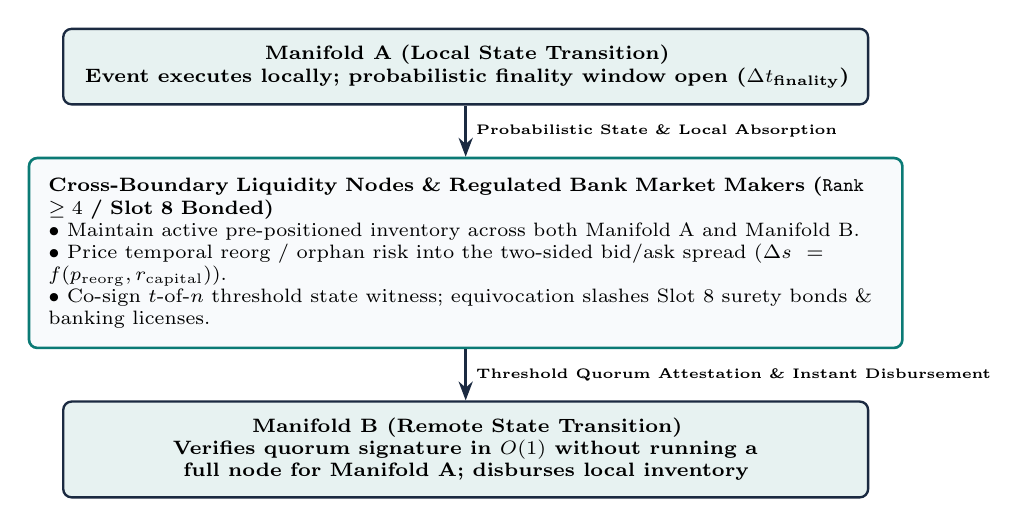
\begin{tikzpicture}[
  node distance=0.65cm,
  manbox/.style={draw=ink, fill=accent!10, rounded corners=3pt, line width=0.85pt, font=\scriptsize\bfseries, align=center, inner sep=6pt, text width=9.8cm},
  mmbox/.style={draw=accent, fill=codebg, rounded corners=3pt, line width=0.95pt, font=\scriptsize, align=left, inner sep=7pt, text width=10.6cm},
  arrow/.style={-{Stealth[length=2.4mm]}, line width=0.9pt, draw=ink}
]
  \node[manbox] (mA) {Manifold A (Local State Transition)\\Event executes locally; probabilistic finality window open ($\Delta t_{\text{finality}}$)};
  \node[mmbox, below=of mA] (mm) {\textbf{Cross-Boundary Liquidity Nodes \& Regulated Bank Market Makers (\code{Rank} $\ge 4$ / Slot 8 Bonded)}\\
  $\bullet$ Maintain active pre-positioned inventory across both Manifold A and Manifold B.\\
  $\bullet$ Price temporal reorg / orphan risk into the two-sided bid/ask spread ($\Delta s = f(p_{\text{reorg}}, r_{\text{capital}})$).\\
  $\bullet$ Co-sign $t$-of-$n$ threshold state witness; equivocation slashes Slot~8 surety bonds \& banking licenses.};
  \node[manbox, below=of mm] (mB) {Manifold B (Remote State Transition)\\Verifies quorum signature in $O(1)$ without running a full node for Manifold A; disburses local inventory};

  \draw[arrow] (mA) -- node[right, font=\tiny\bfseries] {Probabilistic State \& Local Absorption} (mm);
  \draw[arrow] (mm) -- node[right, font=\tiny\bfseries] {Threshold Quorum Attestation \& Instant Disbursement} (mB);
\end{tikzpicture}
\caption{Cross-boundary liquidity architecture: bonded market makers and regulated bank gateways monetize the asynchrony gradient via pre-positioned inventory, insulating protocols from reorg contagion and eliminating custodial lock-and-mint bridges.}
\label{fig:cross_boundary_mm_quorum}
\end{figure}

\begin{enumerate}[nosep]
  \item \textbf{The Spread as the Exact Thermodynamic Price of Reorg Risk:} When a spread opens between Manifold~A and Manifold~B, it is not market inefficiency; it is the exact market price of inventory risk during the asynchrony window. If a user or enterprise demands instant exit from Manifold~A into Manifold~B without waiting for deep finality, the market maker evaluates block depth on Manifold~A, computes the probability of a state rollback ($p_{\text{reorg}}$) plus the capital cost of locked inventory on Manifold~B, and fills the order immediately from its pre-positioned balance sheet. If Manifold~A reorgs, the arbitrageur's inventory absorbs the loss, never the underlying protocol.
  \item \textbf{Multi-Sovereign Quorum as the Observation Layer:} Because Manifold~B does not inspect Manifold~A's raw memory space, it verifies a threshold attestation signed by an independent quorum of regulated banks and bonded liquidity providers holding active balance sheets on both sides. Colluding to attest a fabricated or rolled-back deposit requires economic suicide: the conspirators' locked Slot~8 surety bonds and statutory banking gateway licenses are automatically slashed across the entire network.
  \item \textbf{Velocity Without Incremental Directional Risk:} When a customer transfers purchasing power from Manifold~A to Manifold~B, the market maker absorbs the asset on Manifold~A (expanding Side~A inventory) and simultaneously disburses its pre-existing liquid asset on Manifold~B (contracting Side~B inventory). The market maker's aggregate net worth remains invariant, plus the spread captured into retained earnings—an internal balance-sheet asset substitution rather than a naked directional bet.
  \item \textbf{Internal Self-Healing via Bidirectional Industrial Flow:} Because real-world trade corridors are reciprocal—Spanish solar energy and produce flowing North while German machine tools and power electronics flow South (\cref{sec:thermodynamic_target2})—counterflow transactions automatically reverse inventory drift. If $1{,}000$~EUR-CBMT moves South at 10:00~AM and $1{,}000$~EUR-CBMT of energy receivables moves North at 2:00~PM, the market maker's inventory on both manifolds returns to baseline internally at \textbf{zero marginal on-chain settlement cost}.
  \item \textbf{Threshold Rebalancing vs.\ Lock-and-Mint Bridge Failures:} When structural trade imbalances cause inventory to drift, market makers do not rebalance on every retail transaction. They allow inventory to fluctuate within defined risk bands, dynamically skewing their bid/ask quotes to pay the market to rebalance them organically, and only trigger batched slow-path settlement (via Eurosystem Pontes, Project mBridge, or physical cargo delivery) when the imbalance crosses an optimization threshold and interbank/network fees are lowest. This aligns with empirical cross-chain MEV research showing that roughly two-thirds of professional cross-domain volume settles via pre-positioned inventory, and explains why Web3's ``lock-and-mint'' bridges—which immobilized billions in static smart-contract honeypots to issue unbacked synthetic IOUs—suffered over \$2.8~billion in catastrophic insolvency exploits.
\end{enumerate}

\subsection{The Bosphorus Clearing Filter, the Turkish Currency Scissor, and the Atlantic-to-Pacific Axis}
\label{sec:bosphorus_mbridge_corridor}

Extending this circular clearing topology outward transforms the European industrial mesh from a regional sandbox into a high-throughput, non-dollar settlement axis stretching from the Atlantic to the Pacific (\cref{fig:atlantic_pacific_axis}).

\subsubsection{The Turkish Currency Scissor and the Failure of Crypto's Dollar Monoculture}
The structural vulnerability of the Turkish industrial economy—and of comparable manufacturing hubs across the Mediterranean and Eastern Europe—lies in a severe \textbf{currency scissor}:
\begin{itemize}[nosep]
  \item \textbf{The Real-Economy Currency Mismatch:} Under the EU--T\"urkiye Customs Union, European supply chains are the physical lifeblood of Turkish industry (automotive assemblies, steel, textiles, and white goods), with roughly $45\%$ to $50\%$ of Turkish export revenue invoiced in EUR. Conversely, T\"urkiye depends heavily on imported primary energy (oil, LNG) and raw industrial commodities priced overwhelmingly in USD.
  \item \textbf{The Double-Margin Squeeze:} Whenever the US Dollar undergoes interest-rate tightening or volatility while the Euro fluctuates, Turkish manufacturers are squeezed on both margins: dollar-denominated energy input costs surge while euro-denominated export receivables fail to cover the gap when translated through the domestic banking system. The Central Bank of the Republic of T\"urkiye (TCMB) and commercial banks are forced to burn foreign exchange reserves to bridge the gap, locking the Turkish Lira (TRY) into chronic debasement against both anchors.
  \item \textbf{Why Crypto's Dollar Monoculture Fails Real Industry:} Naive Web3 protocols and DAO treasuries routinely treat cross-border settlement as solved simply because USDT and USDC exist, pricing every governance and service pair against a monolithic \code{TOKEN/USD} order book. Handing a USD stablecoin rail to an Istanbul manufacturer trading with a Stuttgart automaker inflicts three compounding penalties:
  \begin{enumerate}[label=(\alph*),nosep]
    \item \emph{Double FX Conversion Bleed:} The European buyer must convert EUR into USD stablecoins, and the Turkish exporter—who needs EUR to pay regional supply chains or TRY for domestic payroll—must off-ramp out of USD, incurring banking spreads, gas fees, and order-book slippage on both legs.
    \item \emph{Re-Importing Extraterritorial Choke Points:} Routing European--Mediterranean trade through USD stablecoins backed by US Treasury bills re-exposes regional industrial commerce to New York correspondent banking bottlenecks and extraterritorial OFAC freezes.
    \item \emph{Blindness to Reciprocal Netting Flows:} Because EU--Turkish trade is deeply reciprocal—German CNC machinery and optics move Southeast while Turkish automotive sub-assemblies and white goods move Northwest—the vast majority of trade volume should never touch the US Dollar or a spot FX order book at all.
  \end{enumerate}
\end{itemize}

\paragraph{Industrial Clearing and the Radicle / RadWorks (\code{RAD}) Corridor Opportunity.}
In the Sovereign Bunny stack, regional trade and open-source infrastructure markets bypass the vehicle-currency trap entirely:
\begin{enumerate}[nosep]
  \item \textbf{Direct Bilateral EUR and TRY Netting:} Turkish and European manufacturers net EUR-denominated export receivables directly against EUR-denominated capital-goods payables within the account-lattice (\cref{sec:netting_engine}).
  \item \textbf{Synthetic Cross-Rate Compression and Tokenized Commodity Claims:} For residual TRY imbalances, atomic PvP/DvP contracts lock exchange rates at the exact millisecond of verified logistics delivery, eliminating overnight Lira inflation exposure. Rather than holding debasing fiat balances to pre-fund energy imports, industrial actors hold tokenized commodity claims, kWh energy vouchers, or compute credits directly in CAR Slot~2.
  \item \textbf{Native Multi-Currency Corridors for Radicle / RadWorks and SLA-NFTs:} When open-source software ecosystems and hardware collectives (such as Radicle Slot~3 seed operators and RadWorks engineering DAOs, \cref{sec:sla_nft}) denominate SLA-NFTs, enclave build quotas, and maintainer bounties directly in \code{RAD/EUR-CBMT}, \code{RAD/TRY-CBMT}, and metered kWh/compute baskets rather than exclusively in \code{RAD/USD}, they unlock direct industrial procurement across European and Mediterranean SMEs without speculative dollar friction.
\end{enumerate}

\subsubsection{Plugging into Project mBridge: The Atlantic-to-Pacific Non-Dollar Settlement Axis}

\begin{figure}[H]
\centering
\resizebox{\linewidth}{!}{%
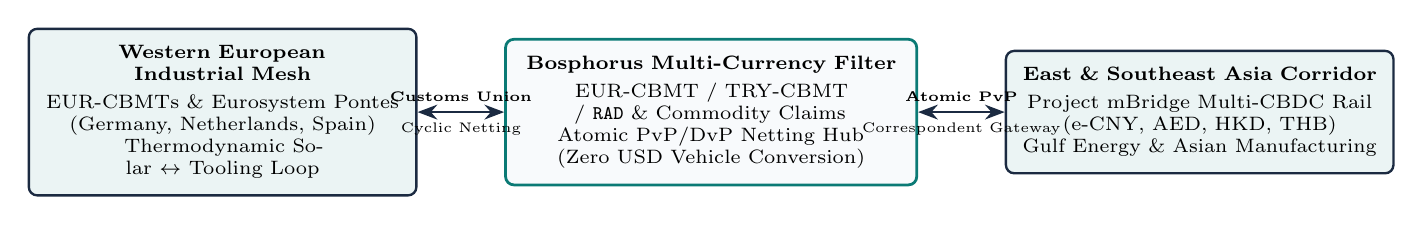
\begin{tikzpicture}[
  node distance=1.0cm,
  axisbox/.style={draw=ink, fill=accent!8, rounded corners=3pt, line width=0.85pt, font=\scriptsize, align=center, inner sep=6pt, text width=4.5cm},
  hubbox/.style={draw=accent, fill=codebg, rounded corners=3pt, line width=1.0pt, font=\scriptsize, align=center, inner sep=6pt, text width=4.8cm},
  biarrow/.style={{Stealth[length=2.5mm]}-{Stealth[length=2.5mm]}, line width=1.0pt, draw=ink}
]
  \node[axisbox] (west) {\textbf{Western European Industrial Mesh}\\[2pt]EUR-CBMTs \& Eurosystem Pontes\\(Germany, Netherlands, Spain)\\Thermodynamic Solar $\leftrightarrow$ Tooling Loop};
  
  \node[hubbox, right=1.1cm of west] (bosphorus) {\textbf{Bosphorus Multi-Currency Filter}\\[2pt]EUR-CBMT / TRY-CBMT / \code{RAD} \& Commodity Claims\\Atomic PvP/DvP Netting Hub\\(Zero USD Vehicle Conversion)};
  
  \node[axisbox, right=1.1cm of bosphorus] (east) {\textbf{East \& Southeast Asia Corridor}\\[2pt]Project mBridge Multi-CBDC Rail\\(e-CNY, AED, HKD, THB)\\Gulf Energy \& Asian Manufacturing};

  \draw[biarrow] (west) -- node[above, font=\tiny\bfseries] {Customs Union} node[below, font=\tiny] {Cyclic Netting} (bosphorus);
  \draw[biarrow] (bosphorus) -- node[above, font=\tiny\bfseries] {Atomic PvP} node[below, font=\tiny] {Correspondent Gateway} (east);
\end{tikzpicture}%
}
\caption{The Atlantic-to-Pacific Non-Dollar Settlement Axis: connecting the European thermodynamic CBMT mesh through the Bosphorus multi-currency clearing filter directly into the Asian and Middle Eastern Project mBridge wholesale corridor.}
\label{fig:atlantic_pacific_axis}
\end{figure}

Geographically and economically positioned at the seam between Europe and Asia, the Bosphorus clearing filter bridges European commercial bank money directly into \textbf{Project mBridge}~\cite{bis2024mbridge} (the multi-CBDC wholesale settlement platform linking the PBOC, HKMA, Bank of Thailand, Central Bank of the UAE, and expanding observer nations):
\begin{itemize}[nosep]
  \item \textbf{Sovereign Interoperability Without Monolithic Lock-In:} German and European commercial banks operating under the DK CBMT framework~\cite{dk2023cbmt} do not need to join a foreign state-controlled blockchain or adopt external regulatory software stacks. Through cross-boundary market-maker quorums (\cref{sec:cross_manifold_mm}), an EUR-CBMT swaps atomically via PvP/DvP against digital Renminbi (\emph{e-CNY}), digital Dirhams (AED), or Hong Kong Dollars (HKD).
  \item \textbf{Direct Physical Terms of Trade:} European industry gains frictionless settlement for Gulf energy and Asian intermediate processing without routing through CHIPS or Fedwire in Manhattan, while Asian and Middle Eastern enterprises settle high-end European machine tools, semiconductor lithography components, and medical devices directly in producer currencies.
  \item \textbf{Dismantling the Correspondent Toll Monopoly:} By combining (1)~intra-European thermodynamic netting (Spanish solar and agrivoltaics retiring German TARGET2 claims), (2)~Bosphorus multi-currency scissor compression, and (3)~atomic wholesale PvP into Project mBridge, international supply chains cease to pay a private rent-extraction toll to a handful of Wall Street money-center banks. Global trade reverts to what it structurally is: a distributed, asynchronous graph of specialized industrial balance sheets settling obligations deterministically against physical delivery.
\end{itemize}

% ============================================================================
\section{Sybil resistance: Proof of Merit, TinyMeritRank, and sociostasis}
\label{sec:sybil}

The consensus and governance layer completely decouples network throughput admission
from reputation-weighted authority.

\subsection{The Mathematical Engine: Personalized PageRank}

\begin{figure}[H]
\centering
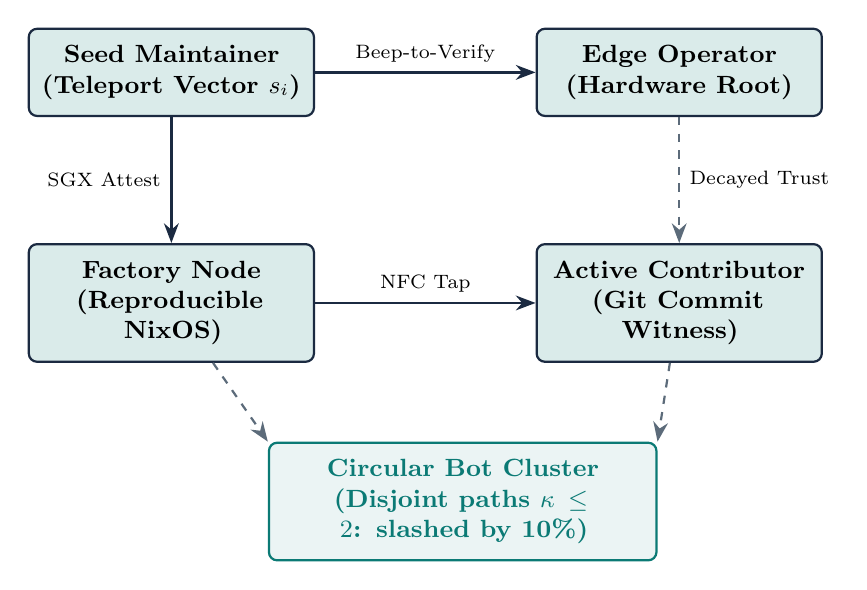
\begin{tikzpicture}[
  node distance=1.6cm and 2.8cm,
  trustnode/.style={draw=ink, fill=accent!15, rounded corners=3pt, line width=0.8pt, font=\small\bfseries, align=center, inner sep=6pt, text width=3.2cm},
  botnode/.style={draw=accent, fill=accent!8, rounded corners=3pt, line width=0.8pt, font=\small\bfseries, align=center, inner sep=6pt, text width=4.5cm, text=accent},
  arrow/.style={-{Stealth[length=2.5mm]}, line width=0.9pt, draw=ink},
  decayarrow/.style={-{Stealth[length=2.5mm]}, line width=0.8pt, draw=mute, dashed}
]
  \node[trustnode] (seed) {Seed Maintainer\\(Teleport Vector $s_i$)};
  \node[trustnode, right=of seed] (edge) {Edge Operator\\(Hardware Root)};
  \node[trustnode, below=of seed] (factory) {Factory Node\\(Reproducible NixOS)};
  \node[trustnode, below=of edge] (contrib) {Active Contributor\\(Git Commit Witness)};
  \node[botnode, below right=1.0cm and -0.6cm of factory] (bot) {Circular Bot Cluster\\(Disjoint paths $\kappa \le 2$: slashed by 10\%)};

  \draw[arrow] (seed) -- node[above, font=\scriptsize] {Beep-to-Verify} (edge);
  \draw[arrow] (seed) -- node[left, font=\scriptsize] {SGX Attest} (factory);
  \draw[decayarrow] (edge) -- node[right, font=\scriptsize] {Decayed Trust} (contrib);
  \draw[arrow] (factory) -- node[above, font=\scriptsize] {NFC Tap} (contrib);

  \draw[decayarrow] (factory) -- (bot.north west);
  \draw[decayarrow] (contrib) -- (bot.north east);
\end{tikzpicture}
\caption{Personalized PageRank trust propagation: physicalized trust propagation and topological bot squelching.}
\label{fig:pagerank_propagation}
\end{figure}

Reputation is directed, subjective, and Sybil-resistant, combining Personalized PageRank~\cite{page1999pagerank} with EigenTrust topological weighting~\cite{kamvar2003eigentrust} and the formal Sybil-bounding foundations of \textbf{MeritRank}~\cite{nasrulin2022meritrank} (\cref{fig:pagerank_propagation}). As proved by Nasrulin, Ishmaev, and Pouwelse~\cite{nasrulin2022meritrank}, aggregating participant feedback via random walks over peer dependency graphs mathematically limits the maximum reputation an adversarial Sybil cluster can extract from the network, eliminating the need for invasive centralized KYC identity verification:
\begin{equation}
R_i(j) = (1 - d) \cdot s_i(j) + d \cdot \sum_{k \to j} \left( \frac{w_{kj}}{\text{Out}_k} \right) R_i(k)
  \label{eq:pagerank}
\end{equation}
Where:
\begin{itemize}
  \item $d = 0.85$ is the damping factor representing the probability of traversing the trust graph.
  \item $s_i(j)$ is observer $i$'s personalized teleport vector, anchoring reputation
relative to observer $i$'s designated peers and preventing global plutocratic capture.
  \item $w_{kj}$ encodes physical ``Beep-to-Verify'' interactions, co-committee evaluations,
and machine maintenance heartbeats.
\end{itemize}

\subsection{Hard-Coded Topological and Temporal Decay}

\begin{enumerate}
  \item \textbf{Topological Attenuation:} If the maximum number of node-disjoint paths
between observer $i$ and node $j$ satisfies $\kappa(i, j) \le 2$, reputation is attenuated:
\begin{equation}
R_i(j) \leftarrow 0.90 \cdot R_i(j)
\end{equation}
This structurally squelches isolated bot-farms and reciprocal vouching rings.
  \item \textbf{Temporal Decay:} A monthly decay rate $\gamma = 0.05$ enforces continuous
operational maintenance. Accumulated reputation evaporates without verified work.
\end{enumerate}

\subsection{Stateless ZK-Merit Verification and AI-Evaluated Contributions}
\label{sec:zk_merit_engine}

To translate continuous topological reputation into concrete governance authority without polluting base ledger state, the system implements a \textbf{5-Tier Fractal Governance and Merit Classification} (\code{crates/identity/src/zk\_merit.rs}):
\begin{itemize}
  \item \textbf{Tier 1 (Public User, Score $\ge 0$):} zkOIDC / ephemeral passkeys; authorized to read content feeds and post in open channels.
  \item \textbf{Tier 2 (Contributor, Score $\ge 500$):} Active code or forum contributors; curate tags and write to shared tables.
  \item \textbf{Tier 3 (Validator, Score $\ge 2{,}500$):} Staked nodes with verified TEE enclaves; sequence Paxos batches and earn epoch distributions.
  \item \textbf{Tier 4 (Treasury Custodian, Score $\ge 10{,}000$):} Threshold multi-signature custodians; authorize treasury allocations and cross-chain interfaces.
  \item \textbf{Tier 5 (Core DevOps / Root Infra, Score $\ge 50{,}000$):} Root cluster maintainers; sign measured kernel enclaves and schema migrations.
\end{itemize}
Contributors prove their tier statelessly using a \textbf{Noir ZK-Merit Proof} ($\pi_{\text{merit}}$) verified in RAM against a LeanIMT / Poseidon Merkle root of the DAO merit tree committed on the DAO account tip. A blinded nullifier prevents cross-channel tracking.

Furthermore, autonomous \textbf{AI Evaluator Agents} running inside TEE enclaves evaluate pull requests, governance forum debates, and community education (\path{crates/consensus/src/system_contracts/ai_merit.rs}), signing deterministic \code{EvaluatedContribution} attestations that mint non-transferable soulbound merit tokens (\code{SOV\_merit}) and dynamically advance contributors along the MeritRank curve.

\subsubsection{TinyMeritRank Rust Algorithm Implementation: from a Single Root to a Seed Set}
\label{sec:multiseed}

In the original MeritRank formulation~\cite{nasrulin2022meritrank} there is no global root:
random walks originate from an observer's subjective seed set (or a consortium's collective seed
set), and Sybil tolerance is enforced by bounding both parallel feedback and the number of
node-disjoint paths $\kappa$. Earlier drafts of this booklet (v0.4) printed a listing whose
attenuation test read \code{disjoint\_paths[0][j]}, which silently hard-codes node~0 as one
universal root and contradicts the personalized teleport distribution $s_i(j)$ of
\cref{eq:pagerank}. The listing below replaces it with a seed set drawn from the active
Zanzibar subgraph (Slot~1) of the DAO being evaluated.

\begin{warnbox}{Implementation status}
The code in the workspace (\path{crates/consensus/src/governance/anti_sybil.rs}) computes
Personalized PageRank for a \emph{single observer} (\code{source}) and applies the $\kappa \le 2$ attenuation
relative to that observer. That is observer-relative, but it is not yet multi-seed.
The multi-seed variant below is \stSpec{}; the file path in the earlier listing caption
(\code{tiny\_merit\_rank.rs}) was illustrative and does not exist.
\end{warnbox}

\Needspace{25\baselineskip}
\begin{lstlisting}[language=Rust,caption={Rust Specification: Multi-Seed Subgraph-Relative TinyMeritRank (target: \code{crates/consensus/src/governance/anti\_sybil.rs})}]
pub struct PolycentricMeritGraph {
    pub damping: f64,              // 0.85
    pub temporal_decay: f64,       // 0.05 per month
    pub min_seed_diversity: usize, // e.g. >= 3 distinct seeds in the DAO subgraph
}

impl PolycentricMeritGraph {
    /// `disjoint_paths_from_seed[s_idx][j]` = node-disjoint paths from seed s_idx to node j.
    pub fn compute_subgraph_rank(
        &self,
        seeds: &[usize],         // seeds elected/rotated (VRF) within one DAO subgraph
        seed_weights: &[f64],    // teleport mass per seed; must sum to 1.0
        edges: &[Vec<f64>],      // verified Slot 1 / Beep-to-Verify / Git interaction weights
        disjoint_paths_from_seed: &[Vec<usize>],
    ) -> Vec<f64> {
        let n = edges.len();
        let mut teleport = vec![0.0; n];
        for (idx, &seed_node) in seeds.iter().enumerate() {
            teleport[seed_node] = seed_weights[idx];
        }
        // Precompute out-weights once instead of per (k, j) pair.
        let out_sum: Vec<f64> = edges.iter().map(|row| row.iter().sum()).collect();

        let mut r = teleport.clone();
        for _ in 0..50 { // power iteration
            let mut r_next = vec![0.0; n];
            for j in 0..n {
                let mut sum = 0.0;
                for k in 0..n {
                    if edges[k][j] > 0.0 && out_sum[k] > 0.0 {
                        sum += (edges[k][j] / out_sum[k]) * r[k];
                    }
                }
                r_next[j] = (1.0 - self.damping) * teleport[j] + self.damping * sum;

                // Multi-seed topological attenuation: how many distinct seeds
                // reach j over >= 2 node-disjoint paths?
                let connected_seeds = (0..seeds.len())
                    .filter(|&s| disjoint_paths_from_seed[s][j] >= 2)
                    .count();
                if connected_seeds < self.min_seed_diversity {
                    r_next[j] *= 0.90; // single-patron cliques and Sybil rings
                }
            }
            r = r_next;
        }
        r
    }
}
\end{lstlisting}

The diversity test is the structural counter to ``Working Towards the Leader'': a node that pleases one
powerful seed while alienating the others stays at $\text{connected\_seeds} = 1$ and is attenuated by 10\% every
iteration, so high rank requires healthy, disjoint paths across several independent seeds.

\subsection{Dynamic Seed-Set Rotation (DSSR)}

To prevent early maintainers from calcifying into an extractive cartel:
\begin{itemize}
  \item \textbf{Candidate Register:} Nodes operating physical infrastructure with verified
heartbeat uptime $> 99.5\%$ qualify for the candidate pool.
  \item \textbf{VRF Root Selection:} Each epoch, a Verifiable Random Function (VRF) selects
active PageRank root seeds from the candidate pool.
  \item \textbf{Evidence-Based Appeal and Sovereign Court (EASC):} Slashing or peer rejection
requires falsifiable on-chain telemetry~\cite{blum2024lightbook}. Arbitrary rejections without cryptographic evidence are automatically committed as \textbf{Social Slag}, penalizing the accuser's rank. Contested disputes escalate through a rigorous three-tier ladder:
  \begin{enumerate}[label=(\alph*),nosep]
    \item \emph{Tier~1 Algorithmic Re-Audit (Prover Appeal):} The appellant stakes a bonded micro-deposit; a randomly sampled 7-member committee of Soulbound AI Agents re-evaluates the submitted telemetry using an alternate PageRank seed-set to test for topological bias.
    \item \emph{Tier~2 Sovereign Jury (Social Verification):} The appellant presents a physical \emph{Beep-to-Verify} record from at least three high-merit peers who physically attest to their industrial output ($Q$). Jurors are compensated via BASEFEE redirects and slashed if found to participate in circular reporting rings.
    \item \emph{Tier~3 Miner DAO Veto (Physical Supreme Court):} For critical blacklisting disputes, the Miner DAO votes with a 66\% supermajority. Because miners control L1 block sequencing, they can refuse to commit an unjust state update until the dispute is resolved.
    \item \emph{The Restoration Loop:} If the appeal succeeds, the entity issuing the fraudulent accusation faces an automated stake multiplier penalty for subsequent epochs.
  \end{enumerate}
\end{itemize}

\subsection{Authority as a Relationship, Not a Protocol Primitive}
\label{sec:relationship_authority}

At the account-lattice layer there is exactly one universal primitive: an \textbf{Actor} holding a
64-slot Compact Account Register. A human with a smartwatch, a Smart Gachapon terminal, a hackerspace, a
savings bank and a federal state are the same kind of object to the base ledger. ``Country'',
``regulatory authority'' and ``standards body'' are \emph{not} account types. Each is a configured
subgraph of Actors connected by Slot~0 (W3C DID and keys), Slot~1 (Zanzibar tuples committed in a Sparse
Merkle Tree) and Slot~6 (ballot and quorum accumulators). Concretely, v0.5 removes three places where earlier
drafts leaked an institutional concept into a protocol interface: the hard-coded \code{cluster\_authority\_did}
public input of the agent-escrow circuit, the fixed seven-region matrix, and the single-root attenuation test of
\cref{sec:multiseed}.

\paragraph{Bilateral tuples replace unilateral authority.}
In an authoritarian topology, authority is one arrow: \emph{State controls Citizen}. In a relationship graph,
institutional power exists only at the intersection of two tuples, one written by each party:
\begin{center}\small
\begin{tabularx}{\textwidth}{@{}L{2.6cm}L{5.6cm}Y@{}}
\toprule
\textbf{Half} & \textbf{Written by / into} & \textbf{Example tuple} \\
\midrule
Upward appointment & Actor, into its own Slot~1 & \code{dao:sparkasse\_mesh\#appointed\_clearing\_anchor@did:sme\_firm\_a} \\
Downward attestation & Anchor DAO, into its own Slot~1, after checking its local rules (multi-seed rank, TEE quote, Proof of SQL audit) & \code{did:sme\_firm\_a\#gmp\_certified\_dispenser@dao:ba\_fin\_pharma} \\
\bottomrule
\end{tabularx}
\end{center}
A verifier does not check a hard-coded ``authority'' flag. It asks one question:
\emph{prove in zero knowledge that your account has a valid path of tuples in Slot~1, and $\kappa$-disjoint
reputation paths, to the seed set of the DAO network that I have appointed as my trust anchor.} This directly
generalises the risk-adjusted dynamic KYC overlap of the banking sections: neither one KYC provider nor one state
root owns an identity, because the anchor is a choice recorded on both sides.

\paragraph{A matrix with no apex.}
Administrative systems with strong coordination typically combine vertical functional lines (ministries, rails,
standards) with horizontal local blocks (provinces, municipalities). That matrix becomes coercive only when every
vertical and horizontal path converges on one static seed. Modelling DAOs of DAOs over Slot~1 and a seed-set
reputation gives the same coordination geometry without the apex: functional subgraphs (a maintainer guild, a supply-chain netting
ring) and civic subgraphs (a hackerspace, a municipal co-op) overlap, each with its own seed set $S_{\text{DAO}}$ and its own
decay and quorum parameters in Slot~6. An actor may hold roles in several at once. If one network becomes extractive, the actor
revokes its upward tuple, a unilateral single-writer transition requiring no consensus, and re-anchors elsewhere,
backed by the continuous exit drill of the operational tests. The Sovereign Stack's exit guarantee is what makes this
revocation credible rather than rhetorical.

\begin{table}[H]
\centering\small
\begin{tabularx}{\textwidth}{@{}L{3.2cm}YY@{}}
\toprule
\textbf{Dimension} & \textbf{Single-seed hierarchy} & \textbf{Multi-seed relationship graph} \\
\midrule
Competition vector & Please one apex; extreme escalation & Earn disjoint paths to several independent, rotating seeds \\
Metric gaming & Local officials optimise the crude proxy and externalise costs & Closed-loop netting and hardware-anchored telemetry; unbacked output stays an un-netted liability \\
Factional sabotage & Denunciation at zero cost & Accusations without falsifiable evidence are committed as Social Slag against the accuser \\
Exit & None; voice is crushed & Export and restore the full state graph; revoke the upward tuple \\
\bottomrule
\end{tabularx}
\caption{Why plural seeds and bilateral tuples change the payoff matrix.}
\end{table}

\subsection{The Social Slag Ledger: Non-Repudiation Merkle Audit Trails}
\label{sec:social_slag}

In legacy Web3 and decentralized governance architectures, malicious or factional actors
routinely launch asymmetric smear campaigns, frivolous slashing proposals, or baseless peer
rejections at zero personal cost. In Sovereign Stack, every peer accusation, dispute, or
slashing proposal is treated as an active, stateful economic assertion. If an assertion lacks
verifiable cryptographic telemetry (such as an unfulfilled DSLA heartbeat, a provable
cryptographic double-sign, or a violated SLA contract) or is overturned by an automated evidence
verifier, it is permanently logged in the accuser's Slot~1 ReBAC record as \textbf{Social Slag}.

The Social Slag engine enforces mathematical non-repudiation:
\begin{enumerate}
  \item \textbf{Monotonic Slag Penalty:} Accusers accumulate a slag coefficient
$S_{\text{slag}} = \sum_{k} \mu_k \cdot \text{Severity}_k$. This coefficient directly
attenuates the node's TinyMeritRank:
\begin{equation}
R_{\text{eff}}(i) = R_i \cdot e^{-S_{\text{slag}}}
\end{equation}
  \item \textbf{Slag Bond Forfeiture:} Initiating an incident report requires locking a
refundable Vibe Bond. If the accusation is deemed spurious or lacks falsifiable telemetry,
the bond is liquidated into the public goods pool.
  \item \textbf{Cryptographic Non-Repudiation:} Every report is committed into an append-only
Merkle accumulator rooted in the accuser's Slot~0 DID record, preventing denial of past accusations.
\end{enumerate}

\Needspace{25\baselineskip}
\begin{lstlisting}[language=Rust,caption={Rust Implementation: Social Slag Non-Repudiation Ledger (\code{crates/identity/src/social\_slag.rs})}]
use sha2::{Digest, Sha256};

#[derive(Clone, Debug, PartialEq, Eq)]
pub enum SlagIncidentType {
    UnprovokedPeerRejection,
    SpuriousSlashingProposal,
    HeartbeatFalsification,
    GachaponBreachDenial,
}

#[derive(Clone, Debug)]
pub struct SlagRecord {
    pub accuser_did: [u8; 32],
    pub accused_did: [u8; 32],
    pub incident_epoch: u64,
    pub incident_type: SlagIncidentType,
    pub telemetry_cid: [u8; 32],    // Iroh BLAKE3 CID of falsifiable evidence
    pub is_substantiated: bool,
    pub penalty_weight: f64,        // e.g. 0.25 rank attenuation
}

pub struct SocialSlagLedger {
    pub slag_records: Vec<SlagRecord>,
    pub accumulated_slag_root: [u8; 32],
}

impl SocialSlagLedger {
    pub fn process_dispute(
        &mut self,
        record: SlagRecord,
        verified_telemetry: bool,
    ) -> Result<f64, &'static str> {
        if verified_telemetry {
            // Accusation backed by authentic cryptographic telemetry
            return Ok(0.0);
        }

        // Accusation is unsubstantiated: apply permanent Social Slag burn
        let mut hasher = Sha256::new();
        hasher.update(&self.accumulated_slag_root);
        hasher.update(&record.accuser_did);
        hasher.update(&record.incident_epoch.to_le_bytes());
        let new_root: [u8; 32] = hasher.finalize().into();

        self.accumulated_slag_root = new_root;
        self.slag_records.push(record.clone());

        // Returns effective attenuation factor to apply to TinyMeritRank
        Ok(record.penalty_weight)
    }
}
\end{lstlisting}

\subsection{Sociostasis, The Mark Effect, and the Systemic Valuation Integral}
\label{sec:sociostasis}

Traditional financial systems and tokenomics suffer from the \textbf{Matthew Effect}~\cite{bothner2011} (``to him who has, more will be given''), rewarding static capital accumulation and whale cartels. The Sovereign Stack counters this with the \textbf{Mark Effect}~\cite{bothner2011}: dynamically routing merit, issuance, and authority toward active maintainers who sustain the health, operational continuity, and resilience of the network.

To prevent human burnout while preserving decentralized operational continuity, the network models social homeostasis (\emph{sociostasis}) across distinct operational frequencies:
\begin{itemize}[nosep]
  \item \textbf{Human Vitality ($F_h$):} Engagement patterns, tactile NFC interactions, and team harmony. Burnout is treated as a legitimate rest signal, not penalized stagnation. Transparent rest is recognized as a positive state: if a maintainer takes time off, $F_h$ drops, but organizational harmony $H$ remains high.
  \item \textbf{Agentic Tempo ($F_a$):} The processing tempo of the user's Soulbound AI Agent.
  \item \textbf{Intentional Behavioral Synchrony (IBS) (\cref{sec:quantum_social_physics}):} Grounded in human-AI neuroergonomics~\cite{naser2023intentional}, the Soulbound AI Agent deliberately synchronizes its decision cadence with the human's authentic behavioral patterns. During human rest and recovery cycles, the agent acts as an intentional behavioral surrogate, casting verified, non-extractive votes bounded by the human's historical risk profile and CAR Slot~1 ReBAC constraints, honoring biological recovery without surrendering on-chain voice.
\end{itemize}

The systemic valuation integral ($W$) evaluates overall network vitality across an epoch $[t_0, t_{\text{epoch}}]$:
\begin{equation}
  W = \frac{\left( \int_{t_0}^{t_{\text{epoch}}} \sum_{i=1}^n \left( M_i(t) \cdot F_i(t) \cdot H_i(t) \right) dt \right) \cdot (V_t + V_c)}{1 + D}
  \label{eq:valuation_integral}
\end{equation}
Where $M_i \cdot F_i \cdot H_i$ represents the instantaneous resonance of node $i$ (Work $M$, Vitality $F$, and Cultural Harmony $H$), $V_t$ is utility velocity (service exchanges and support missions), and $D \ge 0$ is systemic discordance (governance friction and unaddressed burnout). Crucially, capital velocity $V_c$ (funds deployed via ERC-4626 vaults and ERC-3475 tranches) acts as a \textbf{Harmonic Multiplier}: by deploying capital into maintainer tooling and recovery support, high $V_c$ provides breathing room that dampens discordance $D$ without imposing internal psychological stress.

\subsection{Hybrid Corporate Governance and 8-Year Backloaded Vesting Architecture}
\label{sec:hybrid_governance}

Decentralized governance routinely fails due to whale plutocracy, voter apathy, and misaligned venture incentives. Drawing from transparent corporate governance structures in Norway and digital governance frameworks in Estonia, the Sovereign Stack implements a \textbf{Merit-Augmented Corporate DAO} combining executive agility with merit-weighted democratic accountability~\cite{blum2024lightbook,blum2024vision}:
\begin{enumerate}[nosep]
  \item \textbf{DAO Assembly:} Ratifies macro-parameters, protocol upgrades, and capital allocations via gasless, verifiable on-chain voting. All budgetary data is permanently auditable on an open portal, mirroring Norwegian open-budget principles.
  \item \textbf{Elected Board (Oversight Council):} 7--9 members serving staggered 2-year terms. The council composition balances capital and labor: 80\% elected from combined stake and merit pools (45\% merit-weighted via 12-month decayed $M_i$ aggregates, 35\% stake-weighted), and 20\% reserved for public candidates with verified community trust ($R_i > 0.01$ from 5+ peers). The board oversees strategy and audits executive performance via live-streamed proceedings.
  \item \textbf{CEO (Executive Lead):} Appointed for a 4-year term (renewable once). The CEO executes daily operations with board accountability, utilizing multisig controls and automated telemetry dashboards for agility.
  \item \textbf{Mandatory Conflict-of-Interest Disclosures:} Candidates affiliated with third-party service providers must submit standardized conflict disclosures pre-election. Severe conflicts (e.g., equity in competing closed protocols) disqualify candidates; disclosures are immutably logged on-chain.
\end{enumerate}

\subsubsection{The 8-Year Backloaded Vesting Schedule}

To eradicate mercenary capital dumps and align contributor incentives with multi-generational infrastructure survival, executive and founder token allocations follow an \textbf{8-year strongly backloaded vesting schedule} (\cref{tab:vesting_schedule}):

\begin{table}[H]
\centering\small
\begin{tabularx}{\linewidth}{@{}c c c Y@{}}
\toprule
\textbf{Year} & \textbf{Release \%} & \textbf{Cumulative \%} & \textbf{Strategic Incentive Rationale} \\
\midrule
1 & 0.0\% (Cliff) & 0.0\%   & Demands absolute baseline commitment and verified protocol delivery \\
2 & 12.5\%        & 12.5\%  & Predictable linear release begins \\
3 & 12.5\%        & 25.0\%  & Builds retention across early deployment milestones \\
4 & 25.0\%        & 50.0\%  & Completes initial 4-year cycle; aligns with first major audit milestone \\
5 & 7.5\%         & 57.5\%  & Backloaded tier begins modestly to deter post-cycle abandonment \\
6 & 10.0\%        & 67.5\%  & Stepped escalation rewarding enduring operational stewardship \\
7 & 15.0\%        & 82.5\%  & Asymmetrically rewards late-term endurance and maintainer resilience \\
8 & 17.5\%        & 100.0\% & Largest distribution; aligns long-term executive succession incentives \\
\bottomrule
\end{tabularx}
\caption{The 8-Year Backloaded Vesting Schedule: mitigating mercenary token dumps and enforcing generational commitment to open infrastructure.}
\label{tab:vesting_schedule}
\end{table}

Tokens remain locked in a smart vault governed by DAO threshold keys. Clawback mechanisms apply to unvested allocations for provable performance failure or malice, initiated by the board or ratified via community vote.

% ============================================================================

\section{Supply chain assurance, security realism, and the MVSK}
\label{sec:status}

\subsection{CRA and NIS2 Compliance via Machine-Checked Zero-Knowledge}

European regulations (Cyber Resilience Act~\cite{cra}, NIS2~\cite{nis2}) mandate strict
software bill of materials (SBOM) tracking. In the Sovereign Stack, developers commit
CycloneDX SBOMs into Slot~3. A Noir zero-knowledge circuit evaluates:
(1)~that the Git tree commit hash matches the SBOM root,
(2)~that all dependencies meet SLSA Level~3 provenance, and
(3)~non-membership against an on-chain banned CVE Merkle tree, furnishing automated
compliance proofs without disclosing source code.

\subsection{Hardware Realism: What TEE Enclaves Can and Cannot Do}

Trusted execution environments are valuable security components, but they cannot serve
as an assumed root of trust. Intel SGX has been repeatedly breached by side-channel
attacks: Foreshadow~\cite{vanbulck2018foreshadow}, Plundervolt~\cite{murdock2020plundervolt},
SGAxe~\cite{vanschaik2020sgaxe}, \AE{}PIC Leak~\cite{borrello2022aepic}, and
Downfall~\cite{moghimi2023downfall}. Remote attestation proves what binary executed
and on which TCB level; it does not prove silicon is invincible. We therefore:
(a)~require multi-vendor TEE diversity (SGX, AMD SEV-SNP),
(b)~enforce strict TCB freshness policies, and
(c)~never allow a TEE attestation to substitute for an economic slashing bond.

\subsection{Honest Status of the Reference Implementation}

A static review of our reference codebase revealed that the theoretical design remains
ahead of current code. We publish this status transparently:

\begin{table}[H]
\centering\small
\begin{tabularx}{\linewidth}{@{}l l Y@{}}
\toprule
\textbf{Subsystem / Component} & \textbf{Status} & \textbf{Engineering Gap to Production}\\
\midrule
Blind-note transport, view tags & \stPart & Aztec 1-byte view-tag scanner active; rejects 99.6\% noise prior to decryption\\

Single-writer lattice nonces & \stImpl & Monotonic nonces enforced in MVSK, stateless frames, and CAR registers; cross-curve verified\\
TEE quote verification & \textbf{Regression} & Unverified stubs / debug quotes accepted; real DCAP required\\
Web sign-in verifier & \stImpl & Mock bypass eradicated in prod; nonce and expiry checks enforced; fail-closed locks\\

Zero-knowledge circuits (3) & \stPart & Identity, scope, challenge nonces, and vote commitments constrained; circuits.ts typed\\
Proof of SQL table state & \stPart & Row commitment engine and incremental Merkle accumulator active on CAR Slot 4\\
Eurosystem Pontes DvP gateway & \stPart & pacs.009 credit transfer wire contract and deterministic UTR generation active\\
Supply-chain verifier & \stStub & Real Sigstore verification; exact identity match\\
Snow-family finality & \stPart & Derive parameters; authenticate samples; deterministic ties\\
Reputation and anti-Sybil & \stPart & Topological RTT dispersion, ASN 20\% quotas, and quadratic anti-correlation slashing verified\\
Nullifier set / roots & \stPart & Order-independent Merkle tree with non-membership proofs\\
Data-availability sampling & \stStub & Commitments, random sampling, fraud proofs\\
Fee-funded economics (\cref{sec:econ}) & \stSpec & Endogenous credit ($\Delta M = \Delta Y$); fee splits (70/20/10); storage endowments\\
Exit drill & \stImpl & Operationalized CI exit drill under avatar fuzzing (\path{tests/avatar_fuzz_exit_drill.test.ts}); bit-exact Keccak-256 state-root equality verified after cold rehydration\\
\bottomrule
\end{tabularx}
\caption{Status per component at the time of writing. Monotonic lattice nonces and web sign-in have achieved fail-closed completion; ZK circuits, Proof of SQL, Pontes DvP, and anti-Sybil engines have advanced to hardened partial implementation.}

\label{tab:status}
\end{table}

\subsection{The Minimal Viable Security Kernel (MVSK)}
\label{sec:mvsk}

To guarantee security before public deployment, we define the \textbf{Minimal Viable Security Kernel (MVSK)}:
\begin{enumerate}
  \item \textbf{Single-Writer Lattice Validation:} Strict monotonic sequence nonces and verified account signatures on linear slot state transitions.
  \item \textbf{Fail-Closed Verifiers:} Complete eradication of mock signature bypasses and debug TEE flags from all release builds.
  \item \textbf{Order-Independent Nullifier Tracking:} A cryptographic accumulator preventing double-spending within active epoch windows.
  \item \textbf{Bonded Validator Stakes:} Capital-backed bonds forfeitable on provable equivocation.
\end{enumerate}

\subsubsection{MVSK Core State Machine Implementation}

To guarantee fail-closed enforcement at the node binary boundary, the MVSK execution
kernel operates as a self-contained runtime checking every incoming lattice transition
prior to ledger mutation:

\Needspace{25\baselineskip}
\begin{lstlisting}[language=Rust,caption={Rust Implementation: Minimal Viable Security Kernel State Validator (\code{crates/node/src/mvsk\_kernel.rs})}]
pub struct MvskTransitionRequest {
    pub account_id: [u8; 32],
    pub current_nonce: u64,
    pub proposed_nonce: u64,
    pub target_slot: u8,
    pub slot_delta: Vec<u8>,
    pub ed25519_sig: [u8; 64],
    pub tee_dcap_quote: Option<Vec<u8>>,
    pub nullifiers_to_absorb: Vec<[u8; 32]>,
}

pub struct MvskStateKernel {
    pub active_epoch: u64,
    pub nullifier_accumulator: std::collections::HashSet<[u8; 32]>,
    pub trusted_enclave_mrsigner: [u8; 32],
    pub enforce_strict_tee: bool,
}

impl MvskStateKernel {
    pub fn validate_and_apply(
        &mut self,
        req: &MvskTransitionRequest,
    ) -> Result<[u8; 32], &'static str> {
        // 1. Strict Monotonic Nonce (Eliminates Replay Attacks)
        if req.proposed_nonce != req.current_nonce + 1 {
            return Err("MVSK_ERR: Nonce must strictly increment monotonically");
        }

        // 2. Fail-Closed Cryptographic Signature Validation
        if !verify_ed25519(&req.account_id, &req.slot_delta, &req.ed25519_sig) {
            return Err("MVSK_ERR: Signature verification rejected; zero bypasses permitted");
        }

        // 3. Hardware TEE DCAP Attestation Verification
        if self.enforce_strict_tee {
            let quote = req.tee_dcap_quote.as_ref()
                .ok_or("MVSK_ERR: Hardware TEE DCAP quote strictly required")?;
            if !verify_intel_dcap_quote(quote, &self.trusted_enclave_mrsigner) {
                return Err("MVSK_ERR: TEE quote rejected; debug quotes strictly barred");
            }
        }

        // 4. Order-Independent Nullifier Accumulation (Double-Spend Protection)
        for nullifier in &req.nullifiers_to_absorb {
            if self.nullifier_accumulator.contains(nullifier) {
                return Err("MVSK_ERR: Double-spend detected; nullifier already absorbed");
            }
            self.nullifier_accumulator.insert(*nullifier);
        }

        // 5. Emit Deterministic Slot Root
        Ok(compute_slot_hash(req.target_slot, &req.slot_delta))
    }
}
\end{lstlisting}

\subsubsection{Cross-Curve Monotonic Nonce Enforcement on the Stateless Lattice}

In a heterogeneous, multi-curve stateless ledger accommodating legacy Secp256k1 EVM keys, Ed25519 device keys, and post-quantum ML-DSA (Dilithium) signatures across CAR Slot~0 identities, transaction replays present an expanded attack surface: a signed state-transition frame could be replayed across different curves or past state commitments if transitions were decoupled from an account's monotonic sequence.

To permanently close this vulnerability, the Sovereign Bunny execution core enforces \textbf{cross-curve monotonic nonce validation}:
\begin{enumerate}
  \item \textbf{Uniform Transition Nonces:} Every transition request (\code{MvskTransitionRequest}) and execution frame (\code{StatelessTransitionFrame}) must declare its current settled state nonce ($n_{\text{cur}}$) and proposed sequence nonce ($n_{\text{prop}}$), enforcing the invariant:
  \begin{equation}
    n_{\text{prop}} = n_{\text{cur}} + 1
  \end{equation}
  Any stale, decremented, or non-consecutive nonce ($n_{\text{prop}} \neq n_{\text{cur}} + 1$) triggers an immediate fail-closed revert (\code{MVSK\_ERR: Nonce must strictly increment monotonically}).
  \item \textbf{Cryptographic Public-Input Binding:} The nonces $(n_{\text{cur}}, n_{\text{prop}})$ are prepended directly into the canonical public inputs of the transition digest:
  \begin{equation}
    \mathcal{H}_{\text{transition}} = \operatorname{Blake3}\bigl(\text{"sovereign:mvsk:transition:v1:"} \parallel \text{AccountID} \parallel n_{\text{prop}} \parallel \text{SlotID} \parallel \Delta_{\text{slot}}\bigr)
  \end{equation}
  In ZK UltraHonk circuits and SGX execution frames, the verifier asserts that the proof's public inputs match these exact nonces, preventing an adversary from altering nonces outside of circuit constraints.
  \item \textbf{Anti-Replay Nullification for AI Evaluator Operations:} Autonomous AI evaluator signatures (\path{crates/consensus/src/system_contracts/ai_merit.rs}) are protected against double-minting by: (a)~forbidding self-evaluation ($\text{Contributor} \neq \text{Evaluator}$), and (b)~registering every evaluation digest $\mathcal{H}_{\text{eval}}$ into an on-chain nullifier set in \code{ValidatorRegistry}, preventing re-submission of identical merit attestations.
\end{enumerate}

\subsection{Deconstruction of Table 5 Regressions and Remediation Pathways}
\label{sec:regression_deconstruction}

In an industry plagued by superficial marketing audits and decentralized organizations routinely shipping broken or audited-in-name-only code while feigning production readiness, the Sovereign Bunny project treats an Industrial RFC as an uncompromising forensic artifact. We reject the ``glass house'' fallacy: transparently declaring active regressions and unverified cryptographic stubs in an engineering specification is not an admission of weakness, but the foundational hallmark of high-integrity systems engineering. A codebase that openly catalogs its regressions can be systematically remediated; a protocol that conceals them behind synthetic fallbacks is an active hazard.

Below, we dissect the two critical security regressions identified in \cref{tab:status} and establish their concrete fail-closed remediation pathways:

\begin{enumerate}
  \item \textbf{Regression 1: TEE Quote Verification Bypass:}
In early testing harnesses, the attestation precompile (\code{0x00...0005}) accepted
mock or debug quote bytes with unverified Intel SGX signatures, enabling nodes in
development environments to simulate enclave execution without hardware roots.
\emph{Exploit Vector:} An attacker could forge execution quotes, claiming to execute
SLSA Level~3 reproducible builds while running tampered binaries.
\emph{Remediation Requirement:} Complete removal of debug quote accept flags. The
precompile must link directly to the Intel DCAP Quote Verification Enclave (QVE)
library or an on-chain ECDSA P-256 certificate chain verifier evaluating Intel's
root CA, verifying measured MR-ENCLAVE and MR-SIGNER hashes against on-chain DAO release manifests.
  \item \textbf{Regression 2: Web Sign-In Verifier Mock Bypass:}
The SIWE-OIDC gateway contained an unauthenticated bypass allowing synthetic
signature generation when running unit test suites against headless browsers.
\emph{Exploit Vector:} If deployed to production, an adversary could forge user
signatures across web session endpoints without physical key possession.
\emph{Remediation Requirement:} Enforce fail-closed cryptographic challenge-response.
Every web session must generate an unpredictable 32-byte cryptographic nonce, bind
it to the origin domain, enforce a 60-second validity horizon, and require authentic
ECDSA secp256k1 or Ed25519 signatures issued directly by physical tokens or browser extensions.
\end{enumerate}

\subsection{Formal CycloneDX SBOM AST Parser and Noir Witness Generation}
\label{sec:sbom_witness}

To link the physical Git repository committed in Radicle Slot~3 to the zero-knowledge
SBOM verification circuit, the client execution engine runs an automated AST parser.
The parser ingests CycloneDX JSON / XML manifests, computes normalized SHA-256 digests
over pinned dependency hashes, and formats the witness vectors consumed by Noir:

\Needspace{25\baselineskip}
\begin{lstlisting}[language=Rust,caption={Rust Implementation: CycloneDX SBOM Parser and Noir Witness Generator (\code{crates/crypto/src/sbom\_parser.rs})}]
use sha2::{Digest, Sha256};
use serde::{Deserialize, Serialize};

#[derive(Deserialize, Serialize, Debug)]
pub struct CycloneDxComponent {
    pub name: String,
    pub version: String,
    pub hashes: Vec<CycloneDxHash>,
}

#[derive(Deserialize, Serialize, Debug)]
pub struct CycloneDxHash {
    pub alg: String,
    pub content: String,
}

pub struct SbomWitnessGenerator;

impl SbomWitnessGenerator {
    pub fn generate_circuit_witness(
        components: &[CycloneDxComponent],
        banned_cves: &[[u8; 32]],
    ) -> Result<Vec<u8>, &'static str> {
        let mut hasher = Sha256::new();
        for component in components {
            hasher.update(component.name.as_bytes());
            hasher.update(component.version.as_bytes());
            for hash in &component.hashes {
                hasher.update(hash.content.as_bytes());
            }
        }
        let sbom_merkle_root = hasher.finalize();

        // Verify that no component hash collides with the banned CVE database
        for cve_hash in banned_cves {
            if sbom_merkle_root.as_slice() == cve_hash.as_slice() {
                return Err("CRITICAL: Component matches banned CVE database entry");
            }
        }

        Ok(sbom_merkle_root.to_vec())
    }
}
\end{lstlisting}

% ============================================================================

\subsection{NixOS Packaging, ArgoCD CI/CD, and End-to-End Type Preservation}
\label{sec:nixos_devops}

To satisfy rigorous European industrial compliance and prevent catastrophic supply-chain
drift, the Sovereign Bunny stack enforces hermetic reproducibility across its entire lifecycle:
\begin{enumerate}
  \item \textbf{NixOS Flakes for Cluster and Homelab Nodes:} All system services, dependencies,
compiler toolchains, and enclave runtimes are declared strictly as pure, immutable
NixOS flakes (\code{flake.nix}). This guarantees bit-for-bit reproducible node execution
across both test machines and distributed production hardware.
  \item \textbf{Helm Charts on k3s and ArgoCD GitOps:} Sovereign Bunny nodes deploy as lightweight
Helm pods orchestrated within lightweight Kubernetes clusters (\code{k3s}). Continuous
integration and delivery are governed through ArgoCD GitOps pipelines, where every state
change is bound directly to signed Git commits in Radicle Slot~3.
  \item \textbf{End-to-End Type Preservation:} A critical operational failure of legacy dApps is
schema drift between smart contracts and frontend clients. The Sovereign Stack enforces
\textbf{end-to-end type preservation}: data types and event structures defined in
Solidity and Rust contracts are compiled through code generators into strongly typed
WebAssembly bindings and TypeScript interfaces. If an on-chain contract schema changes,
compiler gates immediately fail across frontend clients before deployment, preventing
runtime breakage.
\end{enumerate}

\section{Physical carrier infrastructure, hardware ecosystem, and accelerated deployment}
\label{sec:terminals}

\subsection{Consumable Bearer Vouchers vs. Active Sovereign Nodes}

The physical layer rejects the smartphone as the primary interface. Smartphones are
extractive surveillance vectors leaking telemetry. Daily commerce demands lightweight,
autonomous artifacts (\cref{fig:carrier_diagram}, with physical hardware artifacts pictured in \cref{fig:badges_intro}).

\begin{figure}[H]
\centering
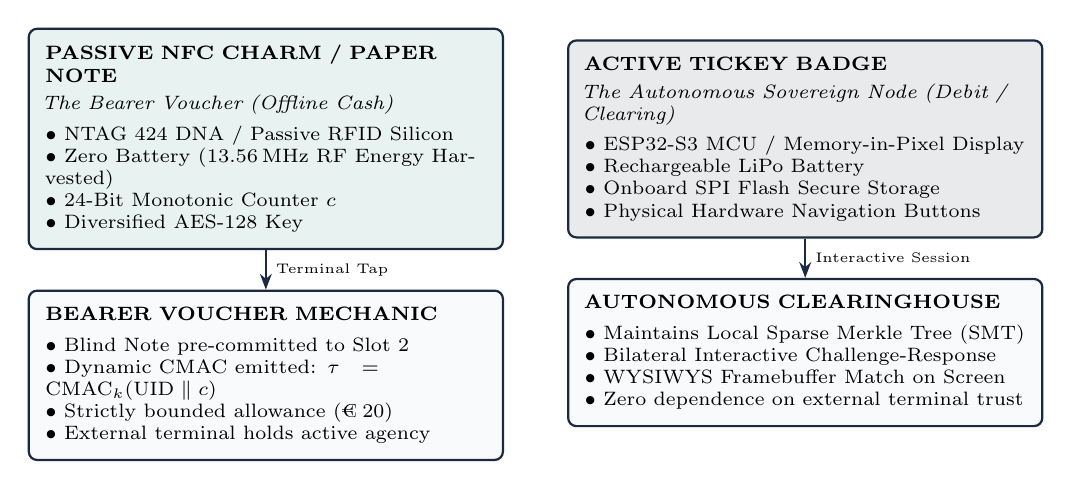
\begin{tikzpicture}[
  card/.style={draw=ink, rounded corners=3pt, line width=0.8pt, inner sep=6pt, text width=5.6cm, font=\scriptsize},
  arrow/.style={-{Stealth[length=2mm]}, line width=0.8pt, draw=ink}
]
  \node[card, fill=accent!10] (lefttop) {
    \textbf{PASSIVE NFC CHARM / PAPER NOTE}\\[2pt]
    \emph{The Bearer Voucher (Offline Cash)}\\[3pt]
    $\bullet$ NTAG 424 DNA / Passive RFID Silicon\\
    $\bullet$ Zero Battery (13.56\,MHz RF Energy Harvested)\\
    $\bullet$ 24-Bit Monotonic Counter $c$\\
    $\bullet$ Diversified AES-128 Key
  };
  \node[card, fill=ink!10, right=0.8cm of lefttop] (righttop) {
    \textbf{ACTIVE TICKEY BADGE}\\[2pt]
    \emph{The Autonomous Sovereign Node (Debit / Clearing)}\\[3pt]
    $\bullet$ ESP32-S3 MCU / Memory-in-Pixel Display\\
    $\bullet$ Rechargeable LiPo Battery\\
    $\bullet$ Onboard SPI Flash Secure Storage\\
    $\bullet$ Physical Hardware Navigation Buttons
  };
  \node[card, fill=codebg, below=0.5cm of lefttop] (leftbot) {
    \textbf{BEARER VOUCHER MECHANIC}\\[3pt]
    $\bullet$ Blind Note pre-committed to Slot 2\\
    $\bullet$ Dynamic CMAC emitted: $\tau = \text{CMAC}_k(\text{UID} \parallel c)$\\
    $\bullet$ Strictly bounded allowance (\EUR{20})\\
    $\bullet$ External terminal holds active agency
  };
  \node[card, fill=codebg, below=0.5cm of righttop] (rightbot) {
    \textbf{AUTONOMOUS CLEARINGHOUSE}\\[3pt]
    $\bullet$ Maintains Local Sparse Merkle Tree (SMT)\\
    $\bullet$ Bilateral Interactive Challenge-Response\\
    $\bullet$ WYSIWYS Framebuffer Match on Screen\\
    $\bullet$ Zero dependence on external terminal trust
  };
  \draw[arrow] (lefttop) -- node[right, font=\tiny] {Terminal Tap} (leftbot);
  \draw[arrow] (righttop) -- node[right, font=\tiny] {Interactive Session} (rightbot);
\end{tikzpicture}
\caption{Physical carrier architecture: structural comparison between passive energy-harvested bearer vouchers and active autonomous clearinghouse badges (physical hardware artifacts pictured in \cref{fig:badges_intro}).}
\label{fig:carrier_diagram}
\end{figure}

\subsubsection{The Passive Bearer Voucher (NTAG 424 DNA)}
\begin{itemize}
  \item \textbf{RF Energy Harvesting:} Zero battery required; powers on via the terminal's
13.56\,MHz carrier wave.
  \item \textbf{Dynamic CMAC Emission:} Auto-increments internal monotonic counter $c$ and emits:
\begin{equation}
\tau = \left( c,\, \text{AES-CMAC}_{K_{\text{tag}}}\bigl(\text{UID} \parallel c \parallel \text{Nonce}_{\text{term}}\bigr) \right)
\end{equation}
  \item \textbf{Sparse Counter Handling:} Accidental pocket taps increment $c$. The ledger's
validation circuit accepts sparse monotonic increments ($c_{\text{new}} > c_{\text{last}}$),
resolving change balances without breaking the state chain.
  \item \textbf{Bounded Blast Radius:} Like a \EUR{20} paper banknote, the maximum loss from
terminal deception or physical theft is strictly bounded to the allowance pre-allocated
to that counter horizon.
\end{itemize}

\subsubsection{The Active Sovereign State Machine (TICKEY / ESP32-S3)}
\begin{itemize}
  \item \textbf{Hardware:} Dual-core Xtensa MCU, 8\,MB SPI flash, long-life LiPo battery,
and sunlight-readable transflective Memory-in-Pixel (MIP) or e-paper display.
  \item \textbf{Local State Engine:} Maintains an internal Sparse Merkle Tree (SMT) representing
local balances and sub-wallets directly in SPI flash.
  \item \textbf{Interactive Challenge-Response:} Receives terminal invoices over dynamic NFC
mailboxes or ESP-NOW mesh bursts.
  \item \textbf{WYSIWYS Display Bus:} Renders counterparty DID and payment amount directly
to the framebuffer over a bare SPI bus. The user presses a physical hardware button,
releasing an Ed25519 signature to authorize the state delta.
\end{itemize}

\subsubsection{Crypto-Native Cash: The 3-Key Consortium Architecture}
\label{sec:crypto_cash_consortium}

To bridge the final mile between decentralized ledger state and daily peer-to-peer physical usability, the Sovereign Stack formalizes \textbf{Crypto-Native Cash} not as an isolated off-chain ledger, but as an on-chain smart account state governed by a \textbf{3-Key Consortium Model}~\cite{blum2024lightbook,blum2024vision}:
\begin{enumerate}[nosep]
  \item \textbf{Key A (Physical Possession):} Hardened NFC chip (e.g., NTAG 424 DNA or secure RFID disc). Written once and locked; signs spending intents under physical tap proximity. Key~A proves possession but cannot unilaterally modify account ownership or policy parameters.
  \item \textbf{Key B (Authority):} Revocable governance capability held by a guardian, parent, merchant consortium, or DAO. Key~B enforces spending thresholds, freezes compromised tags, or authorizes key reissuance.
  \item \textbf{Key C (Ownership Claim):} On-chain smart account or ownership NFT holding ultimate economic title. Key~C can transfer assets, configure policies, or re-assign keys. Physical loss of the tag does not entail loss of funds.
\end{enumerate}

\paragraph{Two Modes of Liquidity Possession.}
Liquidity is partitioned into two distinct operational paradigms:
\begin{itemize}[nosep]
  \item \textbf{Banknote Mode (Object-Bound / Movable):} Value is jailed inside a physical NFC disc. Possession of the physical disc equates to bearer ownership. Under the \textbf{Destroy-to-Settle Rule}, moving these funds to an online account requires redeeming the physical object on-chain, eliminating double-spend risks during offline P2P trade.
  \item \textbf{Badge Mode (Identity-Bound / Fixed):} The NFC chip acts as Key~A within an ERC-4337 smart account, requiring secondary approval (Key~B) for amounts above pre-configured safety thresholds.
\end{itemize}

\paragraph{3-Factor Sovereign Authentication (3FSA) and Social Recovery.}
Access across the physical and digital stack is tiered by risk:
\begin{itemize}[nosep]
  \item \textbf{Something You Have:} The NFC Social Badge / Tiny Disc (low-stakes micro-payments, coffee, Gachapon taps, and physical \emph{Beep-to-Verify} presence).
  \item \textbf{Something You Are/Own:} Smartphone Passkeys / FaceID (active session management, code push to Radicle Slot~3, and ERP review).
  \item \textbf{Something You Know:} Sovereign Passphrase (unlocking high-entropy enclaves, large treasury movements, and actuator kill-switches).
\end{itemize}
If all devices are lost, the user initiates \textbf{Sovereign Social Recovery}: 3 of 5 designated Guardians who have physically \emph{Beep-verified} with the user in the prior 30 days tap their badges to reconstruct the account key via Threshold Secret Sharing (TSS).

\subsection{Tactile Distribution Ecosystem: Physical Nodes, Wearable Signers, and Homelab Watchdogs}

To distribute physicalized tokens, bearer vouchers, and cryptographic credentials without centralized retail infrastructure or cloud custody, the Sovereign Bunny stack grounds distributed consensus in an interconnected physical ecosystem spanning three operational tiers (\cref{fig:monster_badges,fig:gachapon}):
\begin{itemize}[nosep]
  \item \textbf{Ambient Distribution Tier:} Autonomous Smart Gachapon machines and mechanical token dispensers distribute encapsulated Microblock sets, passive e-paper charms, and crypto-native cash on NFC tags directly within hackerspaces, co-ops, and civic gathering points.
  \item \textbf{Tactile Interactive Tier:} Air-gapped wearable signers (PineWatch / PineTime running InfiniTime) establish localized Bluetooth Low Energy (BLE) channels with terminals and merchant POS nodes, requiring conscious physical assent for all cryptographic transfers.
  \item \textbf{Autonomous Oversight Tier:} Self-hosted home-lab nodes monitor local account-lattice streams, generating polynomial column commitments and Proof of SQL audits to detect anomalous spending or state corruption in real time.
\end{itemize}

\begin{figure}[H]
\centering
\begin{subfigure}[t]{0.48\textwidth}
  \centering
  \vspace{0pt}
  
\includegraphics[height=5.2cm, keepaspectratio]{img/monster_epaper_charm.jpg}
  \caption{Physical Passive E-Paper Keychain Charm (Those Who Know Series)}
  \label{fig:monster_charm}
\end{subfigure}\hfill
\begin{subfigure}[t]{0.48\textwidth}
  \centering
  \vspace{0pt}
  
\includegraphics[height=5.2cm, keepaspectratio]{img/those_who_know_monster.png}
  \caption{Authentic Hand-Drawn Character Artwork \& Seat License Archetype}
  \label{fig:monster_art}
\end{subfigure}
\caption{Tactile hardware integration: the ``Those Who Know'' monster series on a miniature passive e-paper NFC keychain charm (left) and its authentic hand-drawn community seat license archetype (right), dispensed via full-node physical Gachapon machines and unlocked into secondary tradability upon SLA expiration.}
\label{fig:monster_badges}
\end{figure}

\subsection{Smart Gachapon Terminal Hardware Architecture and BLE Protocol}
\label{sec:gachapon_hardware}

The Smart Gachapon terminal serves as the ambient bridge between physical commerce
and cryptographic state (\cref{fig:gachapon}). Operating without centralized cloud servers or proprietary
merchant acquiring terminals, the physical deployment integrates:
\begin{itemize}
  \item \textbf{Ambient Mobile NFC Address Resolution (\cref{fig:phone_nfc_scan}):} Standard commodity smartphones equipped with NFC transceivers can read passive NTAG215 / Type~4 transponders or miniature e-paper badges. Reading the tag instantly resolves the target W3C DID and account address (e.g., \code{0x308c...D3e3}) directly into the wallet UI, allowing instant point-to-point Blind Note payments without requiring centralized cloud servers, manual hex entry, or camera-based QR scanning in poor lighting.
  \item \textbf{Tactile Solenoid Tap-to-Dispense (\cref{fig:gachapon_keychain_tap}):} When an authorized user holds their miniature NFC/NFT keychain charm against the ST25R3916 transceiver coil mounted directly over the coin mechanism, the terminal reads the chip's UID and session signature, verifies the payment challenge, and energizes the 12V solenoid to release a physical capsule.
\end{itemize}
Architecturally, the complete vending node integrates:
\begin{itemize}
  \item \textbf{Microcontroller Unit:} ESP32-S3 dual-core Xtensa running at 240\,MHz with 8\,MB PSRAM.
  \item \textbf{NFC Interface:} High-power ST25R3916 or PN532 transceiver driving an amplified
PCB loop antenna, supporting ISO/IEC 14443 Type~A/B and NFC-V.
  \item \textbf{BLE GATT Server:} Emits an advertising beacon (\code{UUID: 0x5056...}) broadcasting
active vending challenges and dispensing session nonces.
  \item \textbf{Physical Mechanism:} Optically isolated 12V DC solenoid actuator releasing
physical capsule merchandise upon verified cryptographic settlement.
\end{itemize}

\begin{figure}[H]
\centering
\begin{subfigure}[t]{0.48\textwidth}
  \centering
  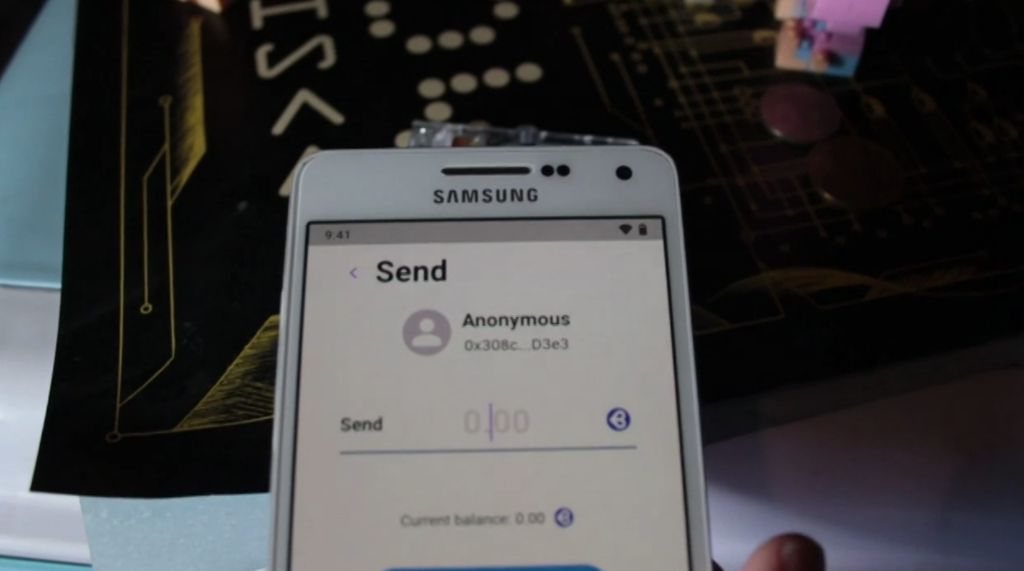
\includegraphics[width=\linewidth,height=4.6cm,keepaspectratio]{img/nfc_phone_scan_address.png}
  \caption{Ambient NFC address resolution: smartphone reads passive NFC tag, displaying resolved recipient address \code{0x308c...D3e3} for point-to-point Blind Note transfer and state synchronization.}
  \label{fig:phone_nfc_scan}
\end{subfigure}
\hfill
\begin{subfigure}[t]{0.48\textwidth}
  \centering
  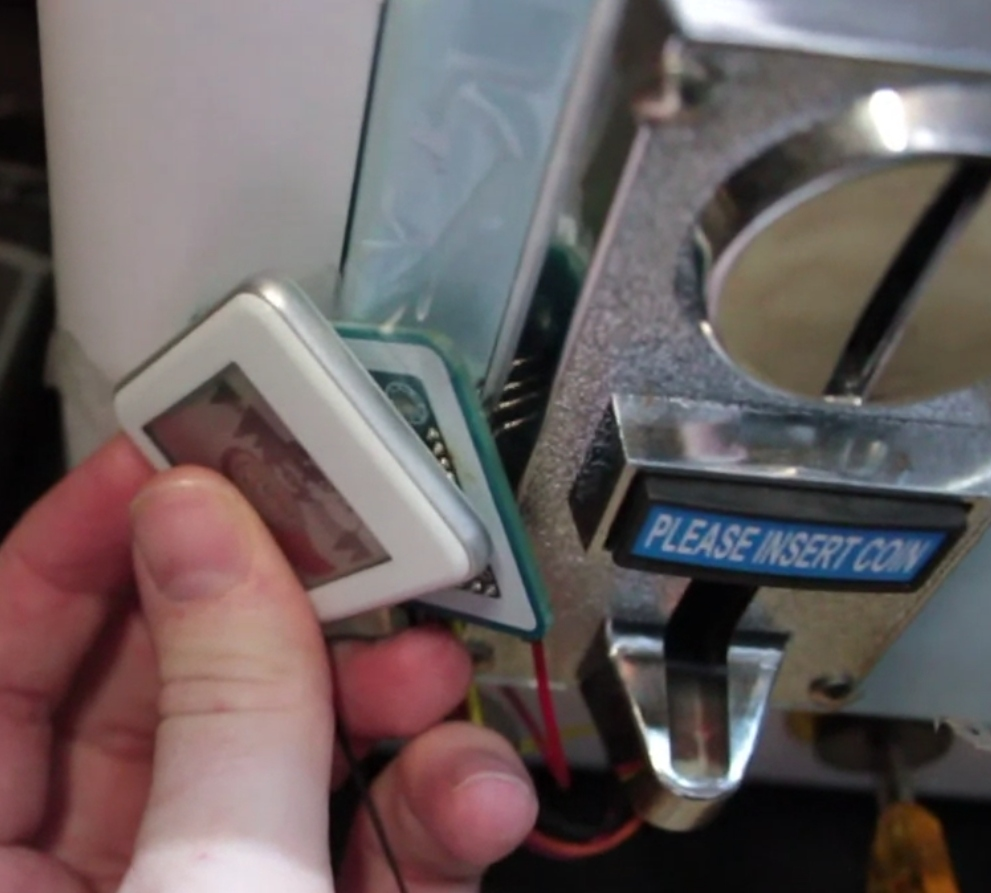
\includegraphics[width=\linewidth,height=4.6cm,keepaspectratio]{img/gachapon_keychain_nfc_tap.jpg}
  \caption{Tactile dispense tap: passive NFC/NFT keychain charm held to the ST25R3916 transceiver coil on the mechanical coin chute to verify session challenge and trigger solenoid capsule release.}
  \label{fig:gachapon_keychain_tap}
\end{subfigure}
\\[8pt]
\begin{subfigure}[t]{0.56\textwidth}
  \centering
  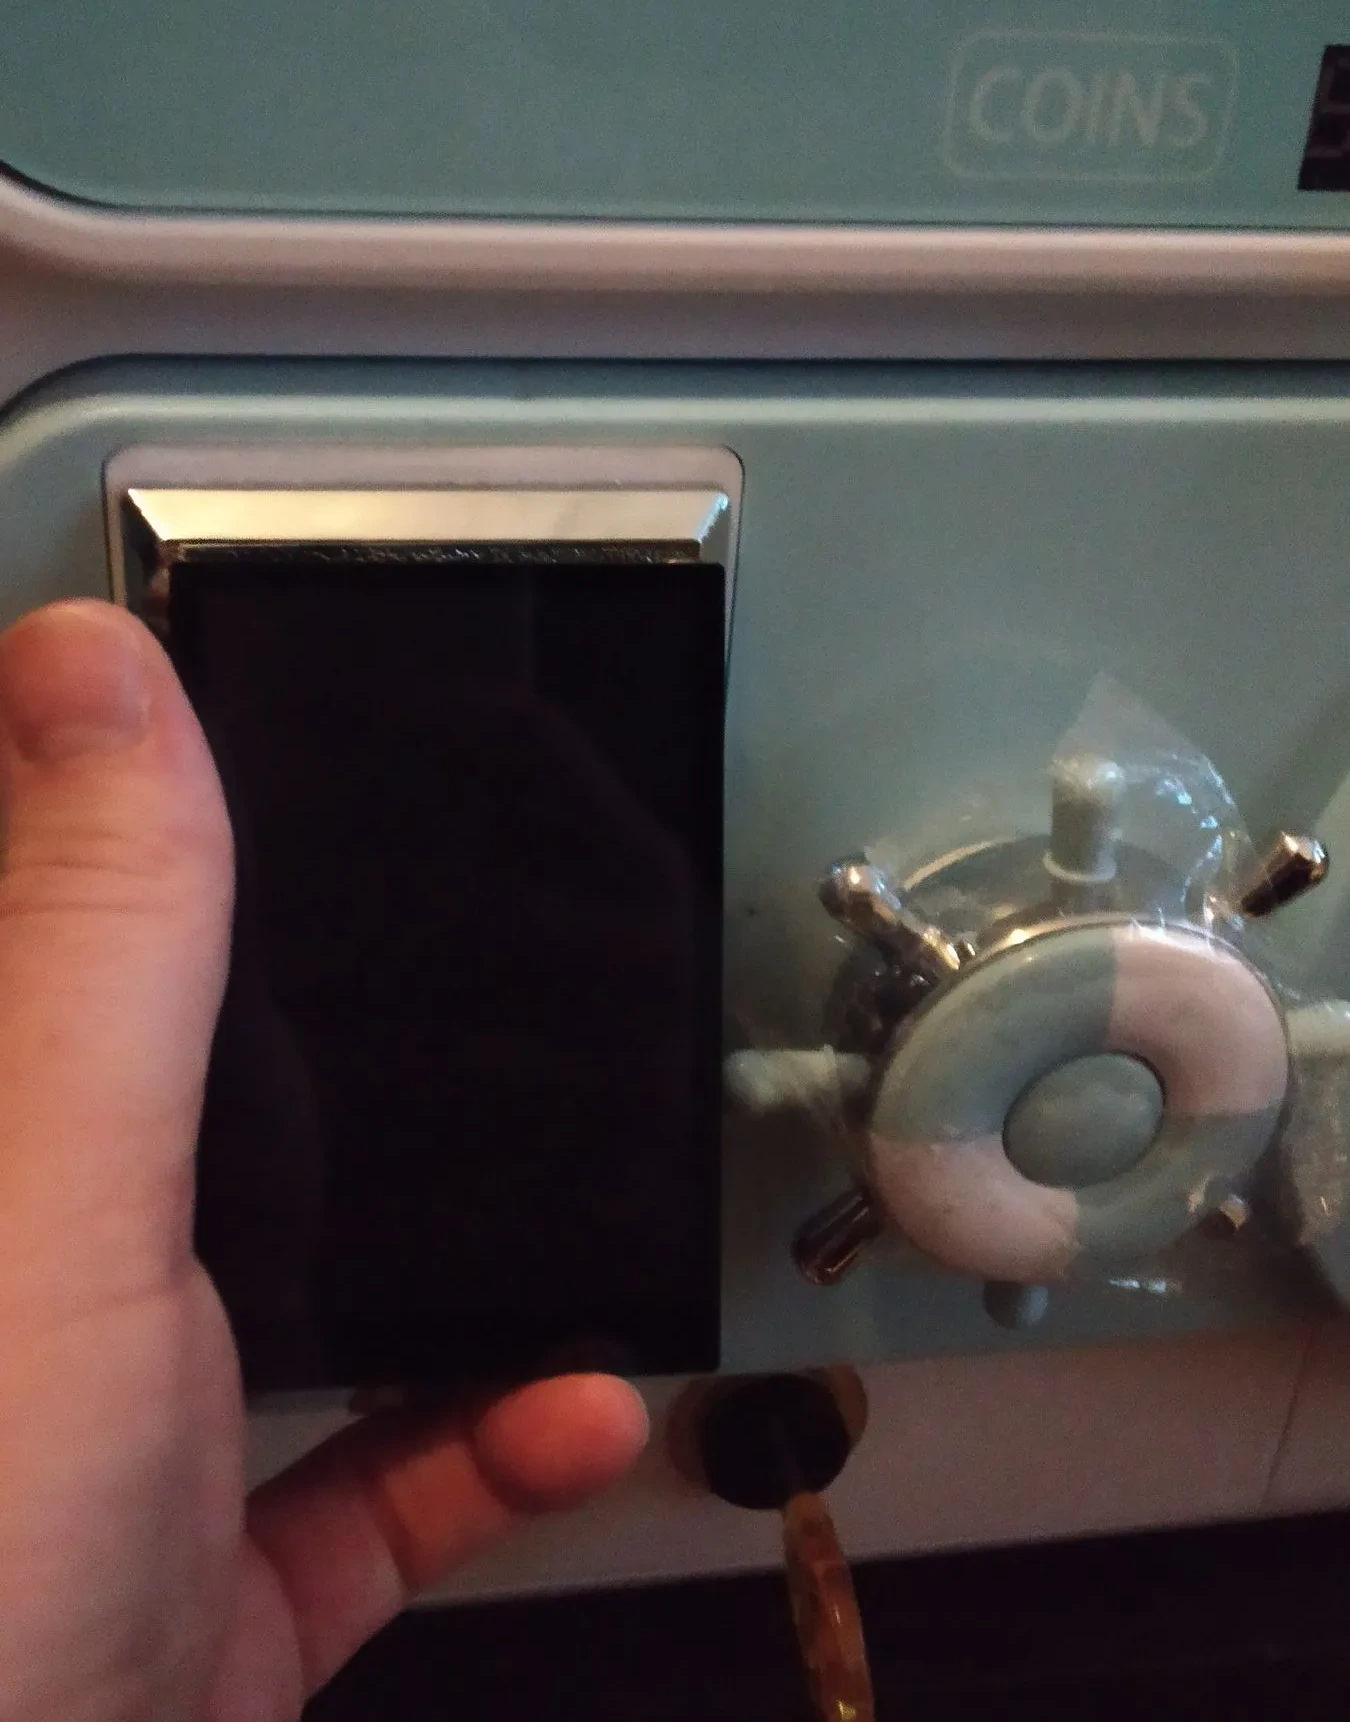
\includegraphics[width=\linewidth,height=7.2cm,keepaspectratio]{img/gachapon.png}
  \caption{Fully assembled autonomous Smart Gachapon distribution terminal featuring custom e-paper display, rotary coin cam, and onboard ESP32-S3 / Linux edge compute node.}
  \label{fig:gachapon_terminal_front}
\end{subfigure}
\caption{The tactile physicalized crypto economy: from ambient mobile peer-to-peer NFC address resolution (a) and hardware charm tap-to-dispense at the coin chute (b) to autonomous edge Gachapon distribution nodes (c).}
\label{fig:gachapon}
\end{figure}

\Needspace{25\baselineskip}
\begin{lstlisting}[language=Rust,caption={Rust Implementation: Smart Gachapon BLE / NFC Exchange Handler (\code{crates/hardware/src/gachapon\_ble.rs})}]
pub struct GachaponSession {
    pub session_id: [u8; 16],
    pub price_eure: u64,
    pub merchant_did: [u8; 32],
    pub terminal_nonce: [u8; 32],
}

impl GachaponSession {
    pub fn verify_wearable_payment(
        &self,
        wearable_signature: &[u8; 64],
        wearable_pubkey: &[u8; 32],
        note_commitment: &[u8; 32],
    ) -> Result<bool, &'static str> {
        // 1. Verify Challenge Digest: H(SessionID || Price || Nonce || NoteCommitment)
        let mut hasher = sha2::Sha256::new();
        hasher.update(&self.session_id);
        hasher.update(&self.price_eure.to_le_bytes());
        hasher.update(&self.terminal_nonce);
        hasher.update(note_commitment);
        let challenge = hasher.finalize();

        // 2. Validate Ed25519 Wearable Signature from PineWatch
        let verified = ed25519_verify(wearable_pubkey, &challenge, wearable_signature);
        if !verified {
            return Err("REVERT: Invalid wearable signature over session challenge");
        }

        // 3. Trigger Physical Solenoid Actuator via GPIO
        trigger_dispenser_solenoid(500); // 500ms pulse
        Ok(true)
    }
}
\end{lstlisting}

\subsubsection{The Two-Machine Physical Gachapon Deployment Architecture}
\label{sec:two_machine_gachapon}

To lower physical deployment barriers while providing an evolutionary path to full crypto-native automation,
the physical Gachapon network is structured into two distinct machine tiers, driven by the \textbf{Tinyblock community} (an open collective of independent \textbf{Microblock} manufacturers, builders, and hackerspaces):
\begin{enumerate}
  \item \textbf{Machine 1 (The Bootstrap Mechanical Token Dispenser):}
  A purely mechanical, zero-power dispensing unit that accepts custom physical minted metal tokens---such as community \textbf{Busy Bee tokens} (distributed during onboarding, purchased with cash at local gatherings, or earned during community merit epochs). It operates with \textbf{zero electrical power and zero Internet connectivity}. When cranked, it dispenses an encapsulated capsule containing:
  \begin{itemize}[nosep]
    \item \textbf{Microblock Sets:} Modular, \textbf{Nanoblock-compatible} construction brick sets, collectible character figurines, and specialized molded assembly elements.
    \item An optional miniature passive e-paper NFC keychain charm pre-flashed with a ``Those Who Know'' series monster badge (\cref{fig:monster_charm}).
    \item \emph{Hardware Boundary Clarification:} Note that raw microcontroller PCBs are \emph{not} dispensed in the standard Gachapon capsules at this stage; microcontroller and embedded PCB integration is reserved for advanced \textbf{DIY Web of Things Tinyblock learning kits}.
  \end{itemize}
  \item \textbf{The Crypto-Native Cash Dispenser Variant:}
  Alongside the brick dispenser, a specialized mechanical variant dispenses \textbf{crypto-native cash on NFC tags} (NXP NTAG 424 DNA keychains or cards pre-loaded with blind notes or seedless cash allowances) paid for with physical custom tokens (\textbf{Busy Bee tokens}), providing a sovereign, permissionless bridge from physical tokens into cryptographic cash without smartphones or POS terminals at the point of dispensation.
  \item \textbf{Machine 2 (The Crypto-Native Smart Dispenser):}
  A modified, smart-vending terminal equipped with an ESP32-S3 microcontroller, high-power ST25R3916 NFC reader, BLE radio, and optical scanner.
Machine~2 accepts direct crypto-native payments: contactless Blind Note NFC taps ($R_2$) or PineWatch BLE authorizations.
Upon cryptographic verification, it energizes a 12V solenoid to dispense the capsule and triggers an on-chain lattice state transition,
binding the newly minted seat NFT directly to the user's DID.
  \item \textbf{Modular Field Upgrade Path:} Community hackerspaces and enterprise offices deploy Machine~1 first with zero upfront
infrastructure overhead. When local connectivity matures, operators bolt on the modular electronic payment controller kit to upgrade
Machine~1 into Machine~2 in minutes.
\end{enumerate}

\subsection{PineWatch / PineTime Autonomous Signing Firmware Protocol}
\label{sec:pinewatch_protocol}

To prevent terminal deception and MitM attacks, the PineWatch (running an open-source
InfiniTime firmware companion) operates with strict display-integrity guarantees:
\begin{enumerate}
  \item \textbf{WYSIWYS Framebuffer Match:} The ESP32 MCU on the PineWatch decodes the
BLE vending payload, rendering the verified merchant DID, the exact settlement amount
(e.g., \EUR{5.00}), and the item description directly to the LCD framebuffer over
a hardware SPI bus.
  \item \textbf{Zero Ambient Execution:} The private signing key resides strictly in the
PineWatch's protected internal flash, never exposed over the BLE radio.
  \item \textbf{Physical Tactile Gate:} The firmware requires a physical push of the watch's
hardware side-button or a double-tap gesture detected by the onboard BMA421
accelerometer, releasing the Ed25519 signature only upon conscious human assent.
\end{enumerate}

\subsection{Homelab Verification Node and Proof of SQL Anomaly Detection}
\label{sec:homelab_agent}

Enterprise operators and privacy-conscious users deploy autonomous verification agents
hosted on self-hosted home-lab infrastructure (fanless x86 mini-PCs running Debian):
\begin{itemize}
  \item \textbf{Continuous Lattice Watchdog:} The agent connects to local P2P Iroh gossip
streams, monitoring state transitions across the user's account slots in real time.
  \item \textbf{Proof of SQL Audit Daemon:} Periodically runs local queries against the
user's ERPNext and PostgreSQL databases, generating polynomial column commitments
and comparing local roots against Slot~4 on-chain digests.
  \item \textbf{Abuse Detection and Wearable Push Alerts:} If an abnormal transaction rate,
unauthorized slot update, or double-spend attempt is detected, the agent immediately
broadcasts an encrypted emergency push notification over WireGuard to the user's
PineWatch, enabling instant one-touch account locking.
\end{itemize}

\subsection{Whole-Stack Supply Chain Arbitrage, the 2026 MIP Patent Cliff, and Stealth Sovereignty}
\label{sec:stealth_sovereignty}

Decentralized physical infrastructure (DePIN) has frequently degenerated into speculative tokens attached to proprietary, closed-source consumer hardware. Conversely, open-hardware initiatives (such as PINE64, InfiniTime, Wasp-OS, and postmarketOS) maintain robust community codebases and lean supply-chain interfaces, but lack the working capital required to finance factory batch tooling and open-silicon runs. The Sovereign Bunny Account-Lattice bridges this gap by acting as a decentralized capital expenditure (CapEx) and supply-chain clearinghouse.

\subsubsection{The Inverted Apple Moat: Cooperative CapEx via Slot~8 Batch Escrows}
Centralized hardware manufacturers deploy CapEx as an anti-competitive weapon: pre-purchasing semiconductor fabrication capacity and financing supplier tooling to enforce proprietary lock-in. Open hardware demonstrates that batch runs of 10{,}000 to 50{,}000 units are economically viable when software development, driver maintenance, and quality assurance are crowdsourced by community maintainers.

The Sovereign Bunny Account-Lattice coordinates this supply chain across three distinct tiers:
\begin{enumerate}
  \item \textbf{The Community Commons (Slot~3):} Operating systems, drivers, and firmware reside in Radicle repositories committed to Slot~3, bound by CycloneDX Software Bills of Materials (SBOM) and reproducible Intel SGX build attestations. Maintainers accumulate non-financialized TinyMeritRank ($M_i$) and receive stream-funded SLA-NFT revenues.
  \item \textbf{Decentralized CapEx \& Factory Tooling Escrow (Slots~4 \& 8):} Community pre-order demand is locked into Slot~8 operational escrows, denominated in Commercial Bank Money Tokens (CBMT-EUR), EURe, or bridged \$RAD / \$TINY surety bonds. Multilateral cyclic netting in Slot~4 cancels mutual claims between printed circuit board (PCB) fabricators, bill-of-materials (BOM) component distributors, and surface-mount assembly houses, funding factory Minimum Order Quantities (MOQs) without venture dilution.
  \item \textbf{Physical Hardware Execution (Layer~0):} Finished devices execute stateless verification locally, communicating via connectionless BLE IPv6 View-Tag filtering without cloud dependencies.
\end{enumerate}

\subsubsection{The 2026 MIP Patent Cliff and Optical OPSEC (``Sovereignpunk'')}
The Sovereign Stack rejects high-refresh AMOLED screens. An AMOLED panel is an active photonic emitter that draws continuous battery power and alerts surrounding cameras and observers whenever a notification arrives. Furthermore, manufacturing 24-bit true-color displays requires dense thin-film transistor matrices that reduce pixel aperture ratios and drive up production costs.

Between 2024 and 2028, the foundational 2004--2008 Japanese patents governing low-power Memory-in-Pixel (MIP) SRAM backplanes expire. This patent cliff allows independent display fabricators to produce 6-bit (64-color) and 8-bit (3-3-2 RGB, 256-color) transflective panels without proprietary licensing royalties:
\begin{itemize}
  \item \textbf{The Pixel-Level Silicon Invariant:} In a transflective MIP panel, each pixel incorporates embedded static RAM latches directly on the glass substrate (1 latch for monochrome, 6 latches for 64 colors, and 8 latches for 256 colors). Because ambient daylight reflects off the backplane, the display requires zero backlight, consuming only 10--15\,$\mu$W in static operation.
  \item \textbf{Optical Operational Security (OPSEC):} In hostile or surveilled environments, a glowing OLED screen acts as an optical beacon. A transflective MIP display emits zero photons, allowing an operator to inspect a What-You-See-Is-What-You-Sign (WYSIWYS) Ed25519 signing challenge or incoming BLE balance delta in total visual obscurity. To an outside observer, the device resembles an ordinary 1990s digital watch; to the operator, it functions as an air-gapped cryptographic signing terminal.
\end{itemize}

\subsubsection{Enterprise Surplus Arbitrage: Datacenter Verification for Under \EUR{200}}
A core advantage of the stateless account-lattice is state compression: because historical transaction graphs are pruned and state transitions are verified statelessly via cryptographic witnesses, the active network state occupies less than 45\,GB of flat memory.

This allows node operators to exploit secondary enterprise hardware surpluses:
\begin{itemize}
  \item Decommissioned dual-socket workstations and rack servers (such as Intel Xeon E5-2600 v2 / LGA~2011 systems with 128\,GB of registered ECC DDR3 RAM and 24 hardware threads) trade for under \EUR{200} on secondary markets.
  \item By dedicating \EUR{180} of surplus enterprise hardware, an operator pins the entire active 64-slot CAR state tree, the in-memory \code{WitnessDatabase}, and the Proof of SQL polynomial evaluators \textbf{100\% in ECC RAM}.
  \item This configuration achieves sub-millisecond cryptographic verification and 4.2\,Ggas/sec parallel execution throughput on consumer-grade budgets, rendering expensive cloud hosting and specialized MEV builder hardware completely obsolete.
\end{itemize}

\subsection{The Infrastructure Cooperation Gap and the Accelerated X-Road API}
\label{sec:xroad_infrastructure}

A pervasive misconception in decentralized networks is that physical hardware or software
represents the primary bottleneck. As our Hardware Bill of Materials (\cref{sec:bom})
demonstrates, optical CWDM transceivers, Supermicro edge servers, and fiber patch cables are
mass-manufactured, cheap, and readily accessible; the software is open source.

The true, debilitating bottleneck is \textbf{institutional cooperation, financing coordination,
and municipal permitting}:
\begin{itemize}
  \item Splicing a new optical dark-fiber strand into city street ducts often requires up to
ten years of bureaucratic filings across fragmented municipal agencies.
  \item Community networks, hackerspaces, and local co-ops are blocked not by engineering limits,
but by legal and administrative barriers of municipal rights-of-way.
\end{itemize}

Sovereign Bunny bridges this gap through an \textbf{Accelerated X-Road API Channel}:
\begin{enumerate}
  \item \textbf{The DAO as Federated X-Road Security Server:} Every participant in the Sovereign Bunny DAO
(such as an open-source hackerspace, community network, or cooperative enterprise) whose daily operations and smart contracts
live on the account-lattice can expose their endpoints through the DAO's federated X-Road gateway. The DAO serves as a certified
European X-Road Security Server, translating municipal REST/SOAP requests into cryptographic lattice assertions.
  \item \textbf{Estonian X-Road Standard Compliance~\cite{xroad2023}:} We implement a decentralized
gateway compatible with the Nordic Institute for Interoperability Solutions (NIIS) X-Road
data exchange layer, the gold standard of European digital governance.
  \item \textbf{Municipal Rights-of-Way Permitting via zkCompliance:} By anchoring contractor bonds
(ERC-3475), civil liability insurances, and certified engineering credentials into Slot~1
and Slot~4, municipal agencies can audit safety invariants and issue fiber-splicing permits
algorithmically via zero-knowledge proofs.
  \item \textbf{Radical Acceleration for Community Nodes:} When an open-source hackerspace or
community node needs fiber spliced into the street, permitting and mutual financing clear
in days rather than decades, grounding digital sovereignty in tangible physical glass.
\end{enumerate}

\section{The Tinyblock manifold: reference implementation of a Sovereign Bunny network}
\label{sec:tinyblock_manifold}

To bridge abstract economic models with visceral physical reality, we document
the reference deployment of a \textbf{Sovereign Bunny Network} operating over a
\textbf{Tinyblock manifold}. \textbf{Tinyblock is a specialized reference instance of the Sovereign Bunny Network}—an autonomous micro-cluster optimized for localized community commerce, 3D modular brick instruction rendering, and physical Smart Gachapon distribution.

Crucially, Tinyblock does not exist in isolation. The Sovereign Bunny architecture is inherently \textbf{multi-instance and meshed}: independent Sovereign Bunny Networks (whether deployed as a community Tinyblock cluster in a hackerspace, an enterprise manufacturing ERP instance, or a municipal clearing hub) seamlessly interconnect over a distributed cryptographic mesh without requiring centralized cross-chain bridges or global state replication.

\subsection{Manifold Topology and Microblock State Model}

In a Tinyblock manifold, transactions do not wait for global consensus blocks.
Each participant (whether a human developer, a Smart Gachapon terminal, or an active
TICKEY badge) advances their local micro-chain by appending signed transition headers:

\Needspace{25\baselineskip}
\begin{lstlisting}[language=Rust,caption={Rust Implementation: Tinyblock Manifold State Header and Transition Engine (\code{crates/node/src/tinyblock\_manifold.rs})}]
pub struct TinyblockHeader {
    pub manifold_id: [u8; 16],
    pub sequence_height: u64,
    pub previous_hash: [u8; 32],
    pub slot_root: [u8; 32],       // 64-slot register Merkle root
    pub note_nullifier: [u8; 32],  // Absorbed blind note nullifier
    pub gas_burnt: u64,
    pub timestamp_ms: u64,
    pub author_did: [u8; 32],
}

pub struct ManifoldState {
    pub current_height: u64,
    pub slot_commitments: [[u8; 32]; 64],
    pub spent_nullifiers: std::collections::HashSet<[u8; 32]>,
}

impl ManifoldState {
    pub fn commit_block(&mut self, block: &TinyblockHeader, sig: &[u8; 64]) -> Result<(), &'static str> {
        // 1. Monotonic Height Progression
        if block.sequence_height != self.current_height + 1 {
            return Err("REVERT: Invalid block sequence height");
        }

        // 2. Nullifier Uniqueness Check
        if self.spent_nullifiers.contains(&block.note_nullifier) {
            return Err("REVERT: Blind note nullifier double-spent");
        }

        // 3. Ed25519 Author Signature Verification
        if !ed25519_verify(&block.author_did, &block.slot_root, sig) {
            return Err("REVERT: Invalid manifold author signature");
        }

        self.current_height = block.sequence_height;
        self.spent_nullifiers.insert(block.note_nullifier);
        Ok(())
    }
}
\end{lstlisting}

\subsection{The 6-Stage Physicalized Workflow}

\begin{figure}[H]
\centering
\begin{tikzpicture}[
  node distance=0.8cm and 0.8cm,
  stage/.style={draw=ink, fill=accent!10, rounded corners=3pt, line width=0.8pt, font=\scriptsize\bfseries, align=center, inner sep=6pt, text width=3.4cm},
  arrow/.style={-{Stealth[length=2.5mm]}, line width=0.9pt, draw=ink}
]
  \node[stage] (s1) {Stage 1: Smart Gachapon\\Mechanical coin turn \& optical capsule dispense};
  \node[stage, right=0.8cm of s1] (s2) {Stage 2: Passive NTAG 424\\NFC tap flashes Genesis Blind Note into Slot 2 (\EUR{20})};
  \node[stage, right=0.8cm of s2] (s3) {Stage 3: TICKEY Badge\\NFC-to-NFC tap absorbs note; WYSIWYS display refresh};

  \node[stage, below=1.0cm of s3] (s4) {Stage 4: PineWatch Wrist\\BLE challenge confirmation; Ed25519 double-tap sign};
  \node[stage, below=1.0cm of s2] (s5) {Stage 5: Homelab Agent\\mini-PC monitors Iroh stream; Proof of SQL ERP verification};
  \node[stage, below=1.0cm of s1] (s6) {Stage 6: zkCompliance\\12ms UltraPlonk audit proof for statutory authorities};

  \draw[arrow] (s1) -- node[above, font=\tiny] {Dispense} (s2);
  \draw[arrow] (s2) -- node[above, font=\tiny] {NFC Tap} (s3);
  \draw[arrow] (s3) -- node[right, font=\tiny] {BLE Ping} (s4);
  \draw[arrow] (s4) -- node[above, font=\tiny] {WireGuard} (s5);
  \draw[arrow] (s5) -- node[above, font=\tiny] {Audit Proof} (s6);
\end{tikzpicture}
\caption{The Sovereign Bunny Manifold Pipeline: End-to-end physicalized flow from Gachapon token emission to wearable signing, homelab anomaly monitoring, and zkCompliance auditing.}
\label{fig:manifold_pipeline}
\end{figure}

The Sovereign Bunny deployment operationalizes daily cryptographic commerce across
six distinct physical stages (\cref{fig:manifold_pipeline}):

\begin{enumerate}
  \item \textbf{Stage 1: Mechanical Capsule Dispense:} A participant inserts a physical
coin into a Smart Gachapon distribution terminal. The mechanical cam turns,
triggering an optical sensor that dispenses a clear plastic capsule containing
an energy-harvested passive NTAG 424 DNA NFC charm.
  \item \textbf{Stage 2: Genesis Tap and NFC Flashing:} The user taps the charm against the
Gachapon terminal's ST25R3916 reader. The machine's onboard ESP32-S3 executes an
on-chain precompile call, flashing a genesis Blind Note into Slot~2. The note
pre-allocates a strictly bounded \EUR{20} consumable bearer allowance.
  \item \textbf{Stage 3: Active TICKEY E-Paper Badge Migration:} The user brings the charm
into contact with their active TICKEY badge. The TICKEY's NFC transceiver executes
a bilateral mutual authentication exchange with the tag, absorbing the passive note
commitment into the TICKEY's local Sparse Merkle Tree (SMT) in SPI flash. The
transflective MIP display instantly refreshes over a direct SPI bus (WYSIWYS),
rendering the updated \EUR{20} spendable balance without connecting to the internet.
  \item \textbf{Stage 4: PineWatch BLE Wrist Signing:} When the user authorizes an outgoing
payment or governance vote, the TICKEY badge broadcasts an encrypted challenge over BLE.
The user's PineWatch vibrates with a distinct haptic pattern. The 240$\times$240
LCD displays the recipient's DID and the exact amount. The user confirms the transaction
with a double-tap wrist gesture or physical button press, releasing an Ed25519 signature.
  \item \textbf{Stage 5: Homelab Policy Agent \& Proof of SQL Monitoring:} An autonomous agent
running on the user's home server (a fanless mini-PC running Debian) monitors the
manifold's Iroh gossip stream. The daemon validates incoming transactions against
the user's ERPNext double-entry ledger, verifying polynomial table commitments in
Slot~4 via Proof of SQL. If an unauthorized state transition occurs, the agent emits an
alert over WireGuard directly to the PineWatch.
  \item \textbf{Stage 6: Statutory Audit via zkCompliance:} When tax inspectors or supervisory
regulators audit the merchant or user, the homelab agent generates a zero-knowledge
audit proof ($\pi_{\text{audit}}$). The proof asserts with mathematical certainty that
all sales tax has been calculated accurately and that inventory matches balance sheets,
without disclosing customer identities, transaction timestamps, or GDPR Article~9 data.
\end{enumerate}

\subsection{Smart Gachapon Terminal: Full-Node Edge Architecture and Proof of SQL Audits}
\label{sec:gachapon_full_node}

Far from being a simplified, microcontroller-driven vending appliance, the physical Smart Gachapon terminal functions as a \textbf{complete, autonomous edge computing node}:
\begin{enumerate}
  \item \textbf{Industrial Hardware Core:} The chassis integrates a high-performance embedded computer (such as a Rockchip RK3588 octa-core ARM64 SoC with 8\,GB LPDDR4x RAM and 128\,GB eMMC/NVMe storage) running a hardened, measured Linux kernel with SGX/TrustZone enclave support.
  \item \textbf{Full Account-Lattice Node:} The machine hosts a native Sovereign Bunny node maintaining its own single-writer account micro-chain, tracking physical capsule inventory, and executing local state transitions in real time.
  \item \textbf{Physical-to-Digital Cash Swaps:} Operating as an ambient neighborhood exchange hub, the terminal accepts physical coins or cash tokens and swaps them into cryptographic blind notes, community mutual credit tokens, or CBMTs. Optical drop sensors verify mechanical dispense events in milliseconds.
  \item \textbf{Autonomous Fiscal Compliance:} With every dispense transaction, the machine calculates and routes statutory value-added tax via the `zkTaxCompliance` pipeline (\cref{sec:zk_tax_compliance}), depositing tax splits atomically to municipal treasury contracts.
  \item \textbf{Proof of SQL Auditability and Legal Recourse:} Local sales, stock levels, and optical dispense logs are committed continuously into an on-chain Proof of SQL Merkle root in Slot~4 ($R_4$). Crucially, Proof of SQL commitments are \textbf{not automatically executed by base consensus}; instead, they serve as unforgeable, publicly inspectable audit trails. Any community member, artist, or tax auditor can inspect inventory balances, file on-chain dispute claims, or initiate zero-knowledge compliance audits with full legal enforceability.
\end{enumerate}

\subsection{The TinyBlock Ecosystem: 3D LDraw Instruction Rendering, zkNFT Blueprints, and Community Fabrication}
\label{sec:tinyblock_ldraw}

To demonstrate how the Sovereign Bunny infrastructure catalyzes creative manufacturing and open-source physical design, the network hosts the \textbf{TinyBlock Ecosystem}: a decentralized platform for modular construction brick sets, architectural models, and anime character figures.

\paragraph{The MobileViT Instruction Parser and 3D LDraw Rule Engine.}
The digitization of physical microblock instructions (Nanoblock, Loz, Tinyblock) into open 3D CAD formats (LDraw~\cite{ldraw2020}) has historically been a labor-intensive, manual process. Standard Optical Character Recognition (OCR) and conventional object detection models fail to capture the hierarchical assembly grammar of block manuals: $\text{Step} \to \text{Layer} \to \text{Brick}$. The Sovereign Stack addresses this via an automated pipeline combining \textbf{Mobile Vision Transformers (MobileViT)}~\cite{mehta2021mobilevit} with a deterministic spatial Rule Engine~\cite{blum2024vision}:
\begin{enumerate}[nosep]
  \item \textbf{Identification vs.\ Placement Separation:} The architecture decouples brick identification in pixel space from assembly placement in 3D vector space. Before detailed parsing, layout analysis classifies the manufacturer template, enabling parallelized step segmentation across threads.
  \item \textbf{Layer~0 Ground Truth (Global Origin):} The center point of the brick assembly in Step~1 is defined as the Global Origin $(0, 0, 0)$ (Ground Truth). All subsequent brick positions are computed as relative displacement vectors from this null point.
  \item \textbf{The Offset Solver:} For each subsequent layer, the model identifies visual markers or ghosted outlines from the preceding step, computing global spatial offsets:
  \begin{equation}
    \text{Offset}_{\text{global}} = \text{Position}_{\text{marker(previous)}} - \text{Position}_{\text{marker(current)}}
  \end{equation}
  The Rule Engine classifies layer mechanics: Minimal ($Z+1$), Standard ($Z+1$ as base $+1$), Multi-Layer, and Studs Not On Top (SNOT / sideways attachment).
  \item \textbf{The 3D Match Fallback (Visual Lock):} In ambiguous orientations or complex rotational steps, 2D calculation triggers a synthetic fallback: the system renders a candidate 3D model from the exact virtual camera angle of the manual, compares the render visually against the 2D illustration, and adjusts $(x, y)$ coordinates in a closed feedback loop (up to 10 rounds).
  \item \textbf{Physics Collision and Stud Alignment Checks:} Before writing to the final LDraw file (\code{.ldr}), physical validation rules verify that studs align with the underlying layer and that no bricks intersect in 3D Euclidean space.
  \item \textbf{Generative Construction via GANs and RL:} By learning the inverse grammar of instruction parsing, the system trains a Generative Adversarial Network (GAN)~\cite{goodfellow2014gan} and reinforcement learning agents to deconstruct arbitrary 3D models into step-by-step physical assembly booklets.
  \item \textbf{Hardware Independence (Edge NPU vs.\ Cloud):} Quantized MobileViT models run locally on consumer devices (Android NPU, iOS CoreML) or within measured edge GPU enclaves over \code{zkSSH}, preserving community autonomy independent of centralized cloud infrastructure.
\end{enumerate}

\paragraph{zkNFT Blueprint Licensing and Community Culture.}
Designers publish their original sets and character archetypes onto the on-chain registry as \textbf{zkNFTs}:
\begin{itemize}
  \item \textbf{Opt-In Proof of License:} Builders can cryptographically prove valid licensing to access authorized physical spare parts, receive priority factory pre-builds, or support the original independent artist. However, proof is completely opt-in; hobbyists can freely inspect, modify, and build sets for personal enjoyment without coercive paywalls.
  \item \textbf{Physical Vending Hubs:} Physical Smart Gachapon machines dispense microblock accessory modules, specialized molded elements, and passive NFC authentication charms.
  \item \textbf{Independent Manufacturing:} Small-scale fabricators license designs directly through smart contracts, producing physical brick sets and sharing revenue with creators via automated fee splits ($s_o, s_c, s_r$), establishing a truly circular cryptographic maker economy.
\end{itemize}

\paragraph{bit.blocks: Modular Electronics, Circuit-Interconnected Microblocks, and Offline Speech Recognition.}
Beyond mechanical construction, Microblocks can be interconnected to create physical electrical circuits through integrated conductive traces, pin headers, and modular brick buses. Operating at the intersection of open hardware and decentralized IoT, \textbf{bit.blocks} provides an accessible, modular physical computing platform:
\begin{itemize}[nosep]
  \item \textbf{Arduino IDE Compatible ESP32 System:} \code{bit.blocks} centers around an ultra-compact ESP32 development core fully compatible with the standard Arduino IDE toolchain and MicroPython, enabling makers to program autonomous agents, local telemetry sensors, and network nodes without proprietary vendor SDKs.
  \item \textbf{Onboard Offline Speech Recognition Chip:} The system integrates a dedicated offline speech recognition processor executing localized keyword spotting, acoustic neural inference, and voice-guided hardware state feedback. All speech processing occurs strictly in-memory on silicon with zero cloud transmission, zero remote API dependencies, and zero eavesdropping risk.
  \item \textbf{Circuit-Interconnected Microblocks:} As illustrated in \cref{fig:bit_blocks_hardware}, Microblock bricks interlock to form modular electronic enclosures, sensor mounts, and visual displays. In this prototype, a Nanoblock-compatible astronaut figurine connects via a modular shielded umbilical harness to a Microblock-encased red LED matrix display module showing real-time digital status telemetry.
  \item \textbf{Educational and Web of Things Roadmap:} While the standard Gachapon machines dispense passive Microblock sets and NFC cash tags, \code{bit.blocks} serves as the hardware foundation for forthcoming \textbf{DIY Web of Things Tinyblock learning kits}, teaching community builders how to construct sovereign hardware nodes, cryptographic keycards, and offline-first sensor networks brick by brick.
\end{itemize}

\begin{figure}[H]
\centering
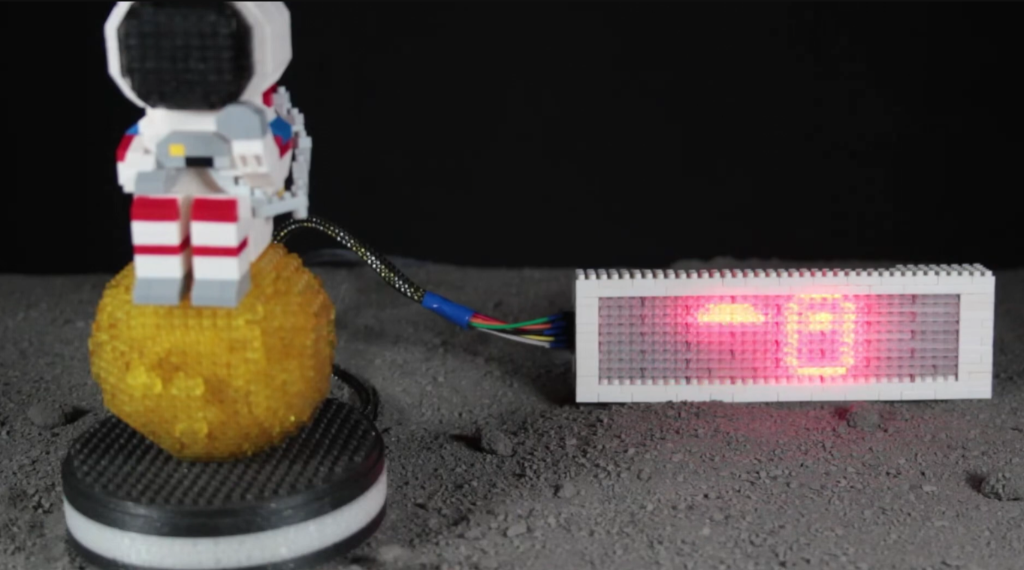
\includegraphics[width=0.88\linewidth]{img/bit_blocks_microblock_display.png}
\caption{\texttt{bit.blocks} modular hardware prototype: an Arduino IDE compatible ESP32 system featuring dedicated offline speech recognition and circuit-interconnected Microblocks. A Nanoblock-compatible astronaut figurine connects via modular cabling to a Microblock-encased LED matrix display module showing real-time digital telemetry.}
\label{fig:bit_blocks_hardware}
\end{figure}

\subsection{Multi-Instance Network Meshing: Sovereign Bunny Inter-Manifold Topology}
\label{sec:manifold_meshing}

The reference implementation implements five interconnected layers to mesh independent Sovereign Bunny network instances into a cohesive economic and cryptographic fabric:

\paragraph{1. Cross-Manifold Relay Mesh via KZG Blobs.}
Routing state diffs and proofs between disparate manifolds operates over EIP-4844 compatible blobs (\path{crates/consensus/src/mesh/relay_mesh.rs}):
\begin{itemize}[nosep]
  \item Packages 131,072-byte polynomial blobs (31 bytes/field element) strictly below the BLS12-381 scalar modulus.
  \item Each packet carries a KZG $G_1$ commitment (48 bytes), proof (48 bytes), and validity proof (Groth16, Binius, or Plonky3).
  \item Unpacks typed intents and enforces \textbf{nullifier replay protection} via on-chain registry \code{processed\_manifold\_messages}.
\end{itemize}

\paragraph{2. Mirrored Chain Mesh Boundary Consensus.}
Cross-chain bridging to legacy transparent monolithic EVM chains operates via mirrored low-entropy interfaces (\code{0x02}, \code{0x03}, \code{0x04}) and the validator mesh (\path{crates/consensus/src/mesh/cross_chain_mesh.rs}, detailed in \cref{sec:cross_chain_blind_notes}):
\begin{itemize}[nosep]
  \item Deterministic low-entropy address registration on the Account-Lattice (\code{0x02} for Ethereum L1, \code{0x03} for Base, \code{0x04} for Gnosis).
  \item Zero-timestamp cryptographic validation via parent hash continuity ($\mathcal{H}_{\text{parent}} = \mathcal{H}_{\text{block}, k}$).
  \item Threshold shard keys (BLS12-381 / FROST) across mesh validators with proofs of possession (\path{pop_signature}).
  \item Stateless verification of legacy MPT witness proofs (\path{eth_getProof}) in \code{WitnessDatabase}.
  \item Direct, native minting of unlinkable Blind Notes ($R_2$) for immediate confidential coordination with zero intermediary VM.
  \item Strict security gating: registering new cross-chain interfaces requires verified \textbf{TinyMerit Rank $\ge 4$}.
\end{itemize}

\paragraph{3. Inter-Manifold BGP Routing and Dataplane Offload.}
Cluster nodes interconnect via a BGP path vector routing daemon (\code{BgpRouter}, \path{crates/consensus/src/mesh/bgp.rs}) over WireGuard tunnels:
\begin{itemize}[nosep]
  \item Dynamically discovers adjacent validator sets and calculates shortest-hop path vectors for routed intents.
  \item Multi-homed peering (\path{crates/consensus/src/mesh/topology.rs}): public ISP transit, 9000-byte jumbo datacenter cross-connects, and DPDK / AF\_XDP offload.
\end{itemize}

\paragraph{4. Address Interest Signaling Swarms.}
Partitions multi-cluster traffic into interest swarms over Iroh-Gossip (\path{crates/network/src/signal_swarm.rs}) to protect edge devices:
\begin{itemize}[nosep]
  \item Nodes maintain an in-memory \textbf{Compressed Cuckoo Filter} with a 256-bit bitmap representation.
  \item Verifies stream subscriptions in $O(1)$ time via Blake3 digests without exposing local address watchlists.
\end{itemize}

\paragraph{5. SIL-3 Actuator Oracles and Hardware Safety Precompiles.}
When cross-instance messages actuate physical hardware (e.g., dispensing Gachapon capsules via \path{crates/consensus/src/system_contracts/actuator.rs}), native precompile \code{0xfe} enforces functional safety:
\begin{itemize}[nosep]
  \item Evaluates \textbf{SIL-3 hardware safety interlocks} and Secure Element signatures before firing actions.
  \item Strict \textbf{200\,ms continuity heartbeat}: link degradation beyond 200\,ms triggers fail-safe \emph{Safe Torque Off (STO)} to prevent physical hazard.
\end{itemize}

\subsection{Network-Scoped Identity and Polycentric Meshes}
\label{sec:scoped_networks}

The five layers above mesh \emph{our} manifolds. A further question is how a node behaves when it belongs to several
networks at once without any of them being ``the'' network. The companion paper
\emph{Radicle Beyond the One Big Room} (\code{docs/booklet/radicle-economic-case.tex}) argues the case in detail for Radicle;
the design points that bind the Sovereign Bunny stack are summarised here. \emph{Status: \stPlan{} unless noted.}

\begin{itemize}
  \item \textbf{Networks are contexts, not places.} A node may be simultaneously in a local BLE or NFC mesh, an isolated Iroh or
        WireGuard ring with a commercial partner, and a selective bridge to public Git refs, with the three never learning of each other.
  \item \textbf{Scoped identifiers.} A network is named by \code{network\_id = BLAKE3(Genesis Trust Manifest)}, covering authorised relay
        keys, cryptographic suites and the Zanzibar schema digest. Identity is rendered \code{did:rad:<network\_id>:<subject>}; the same key yields
        different scoped identities in different networks, and permissions are evaluated only against that network's state. Existing
        \code{did:key} identities stay valid; the current public mesh is \code{did:rad:public}.
  \item \textbf{Handshake firewall.} The first authenticated frame carries the network identifier; a mismatch closes the connection
        before any routing table, inventory announcement or repository reference is exchanged. A cleartext identifier reveals the attempted network,
        so the production construction should prove the binding inside the encrypted session (open problem).
  \item \textbf{Capability-scoped discovery.} Announce an inventory item only to peers for which the relevant Slot~1 tuple holds. This is a
        discovery control, not a substitute for encryption at rest.
  \item \textbf{No hard-coded roots.} Zero default bootstrap connections; directories are opt-in, replaceable subscriptions.
  \item \textbf{Names are claims.} Aliases are scoped by default (\code{alias.mesh\_fingerprint}); a collision across a peering link is a local,
        immediate blocker that forces disambiguation, scoped bridging, or a refusal to route. Canonical (unscoped) names are an optional,
        bonded and non-equivocation-slashable claim on the ledger.
  \item \textbf{Boundary as economic checkpoint.} Inside a cluster trust is dense and cheap; across a boundary, transit is cleared by the cluster's
        aggregate reputation and bonded commitment, so a rogue internal node's blast radius ends at its gateway. Multi-hop intent routing over
        these macro-nodes (\stRes{}) builds on the cross-manifold relay mesh and the multilateral netting of \cref{sec:cross_ledger_netting}.
\end{itemize}

\subsection{Industrial Operations: The Maintenance Shift, Miner's Forge, and Hardware Lifecycle}
\label{sec:industrial_operations}

The physicalization of trust extends beyond vending terminals into heavy industrial infrastructure, energy grids, and hardware sustainability~\cite{blum2024lightbook}:
\begin{enumerate}[nosep]
  \item \textbf{The Maintenance Shift as a Nash Equilibrium:} In conventional industry, maintenance is a cost center to be minimized, causing entropy and infrastructure neglect. The Sovereign Stack formalizes maintenance as an Active Cooperation Equilibrium between Node Operators (Capital) and Maintainers (Labor):
  \begin{itemize}[nosep]
    \item \emph{DSLA Penalty ($P$):} If $P > \text{Cost of Maintenance}$, the operator is financially compelled to fund regular maintenance shifts to prevent slashing.
    \item \emph{Maintenance Salary ($S$):} Funded via BASEFEE redirects and elastic issuance; calibrated to exceed the opportunity cost of negligence, contingent on positive TinyMeritRank.
    \item \emph{Heartbeat Audit ($H$):} Machine Secure Elements sign hardware health telemetry directly; work falsification is impossible. If maintenance ceases, $H$ fails $\implies S$ is withheld; if the operator fails to pay, $H$ fails $\implies P$ slashes capital. Both parties are mathematically coerced into active cooperation.
    \item \emph{The Shift as a Physical Ritual:} The maintainer taps their NFC Social Badge against the machine; the onboard NPU verifies diagnostics; upon returning to ``Green'' status, the proof flushes to the parent rollup, instantly crediting the maintainer's wallet.
  \end{itemize}
  \item \textbf{The Miner's Forge (Geographic Hash-Maps):} Hardware operators voluntarily pin their geographic jurisdiction to an on-chain H3 hexagonal spatial grid (e.g., \code{EU-MEMBER}). This enables the formation of Regional DAOs (such as the EU Miner Bloc) to coordinate collective regulatory defense, carbon tax arbitrage, and shared low-latency fiber infrastructure.
  \item \textbf{Proof-of-Green-Energy (PoGE) Oracles:} Renewable energy meters equipped with hardware Secure Elements emit signed telemetry. The node compiles a zero-knowledge proof asserting 100\% renewable power consumption without exposing physical GPS coordinates or facility IP addresses, unlocking ESG-compliant institutional capital.
  \item \textbf{The Grid-Stabilization Marketplace:} Industrial compute nodes act as high-velocity demand response assets. Miners interface with regional grid operators to provide sub-second frequency tuning (50/60\,Hz) and absorb excess renewable generation, earning curtailment credits while transforming computational facilities into critical public utilities.
  \item \textbf{Hardware Lifecycle DAO and ``Antique Silicon'':} Rather than discarding older ASICs and NPUs after 3 years, the secondary market reroutes mature hardware to heating applications (\textbf{Miner-as-Heater}). In agricultural greenhouses and district heating co-ops, the thermal output of older miners offsets heating costs completely, rendering their effective energy cost of mining zero and providing an unbreakable physical floor for network security.
\end{enumerate}

% ============================================================================

\section{Regulatory verification case study: High-stakes statutory compliance and pharmaceutical supply-chain enforcement}
\label{sec:statutory_compliance}

We examine European statutory pharmaceutical quality control (EU-GMP) and clinical supply-chain verification strictly
as an empirical laboratory of state-machine compliance, regulatory rebound, and the
vital engineering distinction between deadweight bureaucratic friction and
load-bearing safety invariants, not as an endorsement of any particular substance.

Historically, regulated pharmaceutical distribution required multi-part physical paper manifests, fortified vault storage within licensed facilities, and meticulous manual ledger tracking, where minute clerical errors triggered administrative sanctions and supply chain halts. Modern regulatory frameworks seek to decouple pharmaceutical logistics from obsolete paper bureaucracy by introducing standardized electronic prescriptions (\emph{E-Prescriptions}) and automated batch verification.

\subsection{Incentive Alignment and Market Dynamics}

\begin{table}[H]
\centering\small
\begin{tabularx}{\linewidth}{@{}l Y Y@{}}
\toprule
\textbf{Stakeholder} & \textbf{Deadweight Friction Removed} & \textbf{Load-Bearing Friction Retained}\\
\midrule
Pharmacies & Fortified vault paperwork; 3-part carbon slips; punitive liability for clerical transcription errors & Standardized prescription verification; supplier qualification; batch logging\\
Regulators & Heavy court backlogs; policing low-level logistics & Rigorous EU-GMP quality regime; chemical contaminant caps; wholesale import quotas\\
Patients & Short administrative validity windows; societal friction; black-market contamination risk & Mandatory physician indication; statutory prescription gate\\
\bottomrule
\end{tabularx}
\caption{Removal of deadweight friction versus retention of load-bearing safety invariants under statutory pharmaceutical supply-chain regimes.}
\label{tab:compliance_friction}
\end{table}

The economic response across European health systems was immediate. According to official federal monitoring registries, automated digital prescription delivery surged substantially once physical paperwork was digitized. Telemedicine platforms emerged rapidly, connecting patients to licensed physicians and digitizing prescription delivery directly to specialized dispensing pharmacies.

\subsection{Regulatory Rebound: The Cost of Removing Load-Bearing Friction}

However, removing friction indiscriminately introduces severe unintended consequences. When administrative barriers fell without cryptographic state-machine verification, three systemic vulnerabilities materialized:
\begin{enumerate}[nosep]
  \item \textbf{Telemedicine Arbitrage and Questionnaire Approvals:} Telemedicine operators commercialized care, replacing genuine clinical consultations with automated online questionnaires.
  \item \textbf{Lab Shopping and Potency Inflation:} Because price correlates with active ingredient potency, producers pressured testing laboratories to inflate active ingredient percentages and under-report microbial contamination.
  \item \textbf{Cross-Jurisdictional Statutory Antinomy:} Patients holding legitimate prescriptions encountered severe cross-border legal friction (such as driving license investigations under administrative fitness laws) due to lack of verifiable, privacy-preserving proof of legitimate patient status.
\end{enumerate}

\begin{figure}[H]
\centering

\begin{tikzpicture}[
  node distance=1.8cm,
  block/.style={draw=ink, rounded corners=3pt, fill=codebg, line width=0.8pt, font=\scriptsize, align=center, inner sep=6pt},
  friction/.style={draw=accent, line width=1.2pt, fill=accent!8, font=\scriptsize\bfseries, align=center, inner sep=6pt},
  arrow/.style={-{Stealth[length=2.5mm]}, line width=1pt, draw=ink}
]
  \node[block, text width=3.8cm] (gmp) {\textbf{EU-GMP Quality Regime}\\Rigorous batch analysis; chemical contaminant testing; certified lab CoA};
  \node[friction, right=1.2cm of gmp, text width=4.2cm] (friction) {\textbf{The Regulatory Antinomy}\\Medical Privacy (GDPR Art.~9)\\vs.\\Public Safety Verification};
  \node[block, right=1.2cm of friction, text width=3.8cm] (patient) {\textbf{Statutory Patient Protection}\\Legitimate prescription defense; uncompromised civil standing};

  \draw[arrow] (gmp) -- node[above, font=\tiny\bfseries] {Mandatory Proof} (friction);
  \draw[arrow] (friction) -- node[above, font=\tiny\bfseries] {Confidential Assertion} (patient);
\end{tikzpicture}
\caption{The fundamental regulatory antinomy between pharmaceutical quality compliance, patient privacy, and verifiable fitness under statutory health inspection.}
\label{fig:compliance_antinomy}
\end{figure}

\subsection{Decentralized Verification: Zero-Knowledge Association Sets and CAR Integration}

To resolve this antinomy, the Sovereign Bunny architecture implements a \textbf{Zero-Knowledge Association Set Verification Engine} using Noir circuits:
\begin{enumerate}[nosep]
  \item \textbf{Accredited Laboratory Root Attestation:} Certified analytical laboratories post Merkle roots of authentic Certificates of Analysis (CoA) to on-chain CAR Slot~4 (Proof of SQL).
  \item \textbf{Encrypted Dispensing Receipt:} Licensed pharmacies emit a blind receipt to the patient's CAR Slot~2 ($R_2$), referencing the laboratory CoA without linking the patient's public DID.
  \item \textbf{Zero-Knowledge Membership Assertion:} When challenged by regulatory authorities, the patient generates a client-side Noir SNARK proving membership in the authorized patient association set:
  \begin{equation}
    \pi_{\text{patient}} \leftarrow \operatorname{Prove}\Bigl(\operatorname{Batch}_{\text{hash}} \in \operatorname{SMT}(R_{\text{GMP}}) \;\land\; \operatorname{Rx}_{\text{active}} = \text{true} \;\land\; \text{Nullifier} \notin \text{Revoked}\Bigr)
  \end{equation}
\end{enumerate}

\subsubsection{Noir Zero-Knowledge Circuit Implementation}

Below is the concrete Noir circuit specification compiled to Groth16/UltraPlonk, verifying that a presented batch and prescription descend from authorized roots:

\Needspace{25\baselineskip}
\begin{lstlisting}[language=Noir,caption={Noir Circuit: zkCompliance Association-Set Prescriber and Batch Verifier (\code{circuits/src/zk\_compliance.nr})}]
use dep::std::merkle::compute_merkle_root;

fn main(
    // Public Inputs (known to verification terminal)
    gmp_batch_root: pub Field,
    licensed_physician_root: pub Field,
    nullifier_root: pub Field,
    nullifier: pub Field,
    
    // Private Inputs (known strictly to patient's TICKEY badge)
    batch_id: Field,
    batch_merkle_path: [Field; 16],
    batch_index: Field,
    
    physician_id: Field,
    physician_merkle_path: [Field; 16],
    physician_index: Field,
    
    script_secret: Field
) {
    // 1. Assert BatchID belongs to the EU-GMP Certified Importer Root
    let computed_batch_root = compute_merkle_root(batch_id, batch_index, batch_merkle_path);
    assert(computed_batch_root == gmp_batch_root);

    // 2. Assert Prescribing Physician belongs to Statutory Register
    let computed_physician_root = compute_merkle_root(physician_id, physician_index, physician_merkle_path);
    assert(computed_physician_root == licensed_physician_root);

    // 3. Verify Nullifier Uniqueness (Prevents Double-Dispensing)
    let derived_nullifier = std::hash::poseidon([batch_id, script_secret]);
    assert(derived_nullifier == nullifier);
}
\end{lstlisting}

\subsection{On-Site Terminal Verification Protocol and Administrative Law Analysis}
\label{sec:onsite_verification_flow}

To understand how the zero-knowledge verification operates during field enforcement, we trace the interactive NFC handshake executed between a statutory inspection terminal and the patient's TICKEY badge:

\begin{figure}[H]
\centering
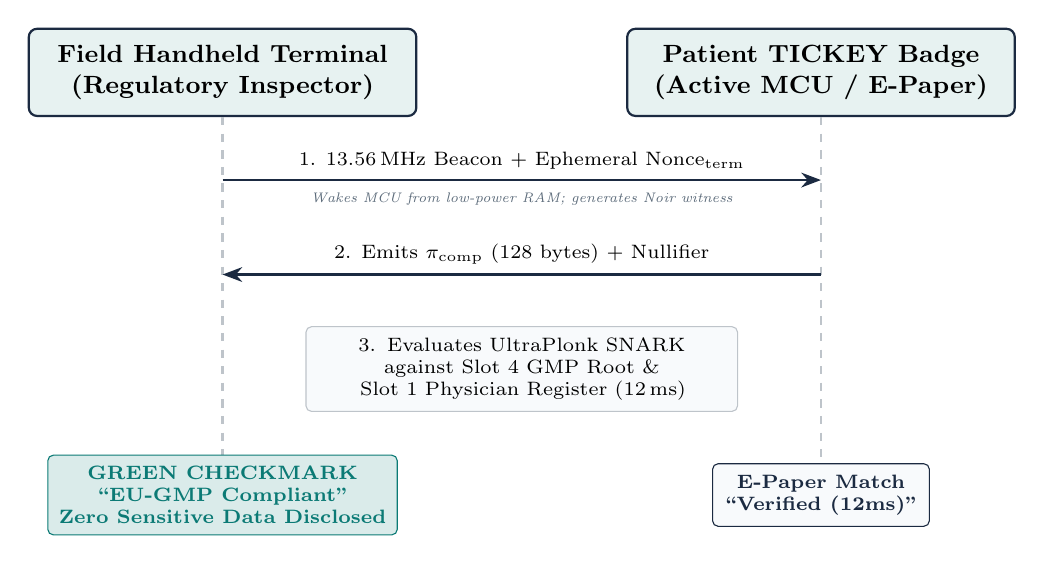
\begin{tikzpicture}[
  entity/.style={draw=ink, fill=accent!10, rounded corners=3pt, line width=0.8pt, font=\small\bfseries, inner sep=6pt, text width=4.5cm, align=center},
  stepbox/.style={draw=mute!40, fill=codebg, rounded corners=2pt, font=\scriptsize, inner sep=4pt, text width=5.2cm, align=center},
  arrow/.style={-{Stealth[length=2.5mm]}, line width=0.9pt, draw=ink},
  dashedline/.style={draw=mute!40, line width=0.8pt, dashed}
]
  \node[entity] (police) at (0, 0) {Field Handheld Terminal\\(Regulatory Inspector)};
  \node[entity] (badge) at (7.6, 0) {Patient TICKEY Badge\\(Active MCU / E-Paper)};

  % Lifelines
  \draw[dashedline] (police.south) -- ++(0, -4.8cm) coordinate (pbottom);
  \draw[dashedline] (badge.south) -- ++(0, -4.8cm) coordinate (bbottom);

  % Steps
  \coordinate (y1) at ($(police.south)+(0, -0.8cm)$);
  \coordinate (y2) at ($(police.south)+(0, -2.0cm)$);
  \coordinate (y3) at ($(police.south)+(0, -3.2cm)$);

  % Step 1: Broadcast
  \draw[arrow] (police.south |- y1) -- node[above, font=\scriptsize] {1. 13.56\,MHz Beacon + Ephemeral $\text{Nonce}_{\text{term}}$} (badge.south |- y1);
  \node[font=\tiny\itshape, text=mute, below=1pt] at ($(police.south |- y1)!0.5!(badge.south |- y1)$) {Wakes MCU from low-power RAM; generates Noir witness};

  % Step 2: Proof emission
  \draw[arrow] (badge.south |- y2) -- node[above, font=\scriptsize] {2. Emits $\pi_{\text{comp}}$ (128 bytes) + Nullifier} (police.south |- y2);

  % Step 3: Evaluation (Centered between lifelines)
  \node[stepbox] at ($(police.south |- y3)!0.5!(badge.south |- y3)$) {3. Evaluates UltraPlonk SNARK against Slot~4 GMP Root \& Slot~1 Physician Register (12\,ms)};

  % Step 4: Display match
  \node[draw=accent, fill=accent!15, rounded corners=2pt, font=\scriptsize\bfseries, text=accent, align=center, inner sep=4pt] at (pbottom) {GREEN CHECKMARK\\``EU-GMP Compliant''\\Zero Sensitive Data Disclosed};
  \node[draw=ink, fill=codebg, rounded corners=2pt, font=\scriptsize\bfseries, text=ink, align=center, inner sep=4pt] at (bbottom) {E-Paper Match\\``Verified (12ms)''};
\end{tikzpicture}
\caption{On-site zero-knowledge inspection handshake: resolving statutory inspection without disclosing patient diagnosis, medical history, or prescribing physician.}
\label{fig:onsite_inspection_flow}
\end{figure}

\subsubsection{Statutory Tension: Administrative Inspection vs. GDPR Article 9}
Under legacy administrative inspection practice, demonstrating compliance with statutory pharmaceutical controls coerced individuals into surrendering their entire medical file to municipal clerks who possess zero clinical clearance.

This practice constitutes a severe conflict with core European legal safeguards:
\begin{itemize}
  \item \textbf{GDPR Article 9 (Special Categories of Data):} Processing of personal health data is strictly prohibited unless covered by narrow statutory exceptions with proportional safeguards.
  \item \textbf{Medical Professional Secrecy:} Compelling individuals to disclose physician consult notes undermines privileged medical relationships.
  \item \textbf{Informational Self-Determination (\emph{BVerfGE 65, 1}):} Citizens must not be forced to reveal intimate medical details to satisfy general administrative fitness checks.
\end{itemize}

By deploying the Sovereign zkCompliance protocol, the patient satisfies the state's legitimate public safety check ($Q_{\text{safety}}$: genuine EU-GMP medication, valid physician license, unspent dispensing quota) while preserving absolute mathematical confidentiality over their person.



\section{Industrial and community use cases}
\label{sec:usecases}

\subsection{Use Case 1: Industrial SME Deployment with Nextcloud and ERPNext}

A European manufacturing SME anchors its existing open-source stack
(Nextcloud~\cite{nextcloud} documents, ERPNext~\cite{erpnext} inventory) into the
Sovereign Account-Lattice (\cref{tab:sql_dashboard}):
\begin{enumerate}
  \item \textbf{Proof of SQL Commitments:} On-premises databases generate polynomial table
commitments over inventory tables, posting digests to Slot~4.
  \item \textbf{Content-Addressed Pinning:} Technical drawings and EU-GMP certificates
managed in Nextcloud are hashed into BLAKE3 roots and referenced in Slot~2.
  \item \textbf{Zero-Knowledge Audits:} Regulatory authorities and lending banks verify
balance-sheet solvency ($\sum \text{receivables} - \sum \text{payables} \ge \text{Debt}$)
via Inner-Product Arguments in milliseconds, without viewing raw customer lists.
\end{enumerate}

\begin{table}[H]
\centering\small
\renewcommand{\arraystretch}{1.2}
\begin{tabularx}{0.95\linewidth}{@{}l L{4.5cm} Y@{}}
\toprule
\textbf{Local Table / File Target} & \textbf{Cryptographic Commitment} & \textbf{Auditor Verification Status}\\
\midrule
ERPNext \code{inventory\_movements} & BLAKE3 Table Root ($S_4$) & $\checkmark$ Proof Valid: Physical Inventory Matched\\
ERPNext \code{sales\_invoices} & Inner-Product Argument & $\checkmark$ Solvency Proven: Zero GDPR Data Disclosed\\
Nextcloud Document Attachments & Iroh BLAKE3 CIDs ($S_2/S_4$) & $\checkmark$ Cryptographic Chain-of-Custody Verified\\
\bottomrule
\end{tabularx}
\caption{Enterprise audit dashboard verifying SQL state transitions and Nextcloud document integrity across open-source SME infrastructure.}
\label{tab:sql_dashboard}
\end{table}

\subsection{Use Case 2: The Third Place: Community Workshop Node}

A community maker cooperative operates a fanless industrial edge mini-PC hosting an
encrypted blind-note cache, local machine authorization registries, and Zanzibar deReBAC
access controls (\cref{fig:derebac_explorer}):
\begin{enumerate}
  \item \textbf{Hardware-Interlocked Tool Access:} High-hazard machinery (such as 5-axis CNC
milling centers, metal lathes, and CO$_2$ laser cutters) are physically interlocked via
industrial ESP32 relay modules. A member initiates machine operation by tapping their
active TICKEY badge or passive NTAG 424 charm. The local edge node verifies the
Zanzibar tuple in Slot~1 (\code{user:alice\#certified\_machinist@tool:cnc\_5axis}) in
under 8~milliseconds, powering the safety contactor.
  \item \textbf{Offline Blind-Note Caching:} During broadband ISP outages or municipal power
grid partitioning, the edge node operates in disconnected local-mesh mode. Members
consume pre-committed blind notes for machine runtime and material stock. Local monotonic
counters prevent replay attacks. Upon WAN reconnection, the node reconciles frontier
hashes over Iroh gossip without requiring global chain rollbacks.
  \item \textbf{Decentralized Infrastructure Co-Op:} Metro dark-fibre colocation and gigabit
backhaul costs (\EUR{810}/month across a regional confederation of 40 community nodes,
equating to \EUR{20.25}/month per workshop) are settled peer-to-peer via automated
cyclic netting, eliminating proprietary SaaS subscription overhead.
\end{enumerate}

\subsection{Use Case 3: Cross-Border Interbank Trade-Finance Corridor}

Cross-border industrial supply chains across the European Single Market and the EU--T\"urkiye Customs Union frequently suffer
from multi-week payment delays, high factoring costs, and structural imbalances in the
Eurosystem's TARGET2 clearing system (\cref{sec:target2_balancing}). In a multi-corridor supply chain spanning Germany, the Netherlands, Spain, Northern Italy, and T\"urkiye:
\begin{enumerate}
  \item \textbf{Statutory Ingestion and Invoice Anchoring:} Suppliers register VAT-compliant
e-invoices in their respective national ERP systems (e.g., ERPNext, SAP), posting BLAKE3
column commitments to Slot~4.
  \item \textbf{Cross-Border Cyclic Debt Netting:} The multi-tier netting engine
(\cref{sec:netting_engine}) executes cyclic reduction across international boundaries.
Gross cross-border trade debt of \EUR{48,000,000} compresses to a net residual of
\EUR{7,600,000} (an 84.1\% reduction in required interbank liquidity).
  \item \textbf{Arresting TARGET2 Divergence and Thermodynamic Offtake:} Because bilateral obligations are extinguished
endogenously within the private sector prior to interbank settlement, gross central bank
claims between the Deutsche Bundesbank, the Banco de Espa\~na, and the Banca d'Italia are minimized. Long-horizon capital equipment leases (e.g., German HVDC and semiconductor hardware combined with Dutch greenhouse automation deployed into Spanish solar and agrivoltaic parks) amortize continuously via signed kWh and produce delivery attestations (\cref{sec:thermodynamic_target2}), while residual cash legs settle atomically via commercial bank gateways over the Eurosystem Pontes Trigger bridge into TIPS and outward across the Bosphorus multi-currency filter into Project mBridge (\cref{sec:bosphorus_mbridge_corridor}).
\end{enumerate}

\subsection{Use Case 4: Sovereign Forge Hosting with a Commons and Commercial Layer}

Open-source developers have repeatedly suffered from platform enclosure, arbitrary account
suspensions, and unilateral licensing changes on centralized forges. The Sovereign Stack
decouples forge collaboration into an open commons protocol and a competitive commercial layer:
\begin{enumerate}
  \item \textbf{Radicle Slot 3 State Anchoring:} Canonical Git repository references, release
tags, and SLSA Level~3 SBOM compliance proofs reside immutably on the Sovereign
Account-Lattice (\cref{tab:dao_release_ui}).
  \item \textbf{Dual-Tier Infrastructure Provisioning:} Non-profit maintainer communities operate
volunteer seed nodes over the peer-to-peer Iroh transport. Simultaneously, commercial
cloud hosting providers offer high-availability seeds, automated CI/CD runners inside
Intel SGX enclaves, and enterprise SLAs financed via Dynamic SLA NFTs (\cref{sec:sla_nft}).
  \item \textbf{Sovereign Exit Guarantee:} Both volunteer and commercial providers serve from
the identical cryptographic state in Slot~3. If a commercial host degrades latency,
censors repositories, or increases hosting rates, maintainers switch their DNS and
P2P discovery endpoints with zero downtime, preserving all commits, cryptographic
signatures, and issue threads without data loss.
\end{enumerate}

\begin{table}[H]
\centering\small
\renewcommand{\arraystretch}{1.2}
\begin{tabularx}{0.95\linewidth}{@{}l L{4.5cm} Y@{}}
\toprule
\textbf{Target Reference} & \textbf{Delegate Threshold} & \textbf{Supply Chain Attestation}\\
\midrule
\code{refs/tags/v2.4.0} & 3-of-5 MuSig2 Verified & $\checkmark$ CycloneDX SBOM Attested (SLSA L3)\\
\code{Commit: 0x8f2a...} & Slot Nonce: \code{h+1} & $\checkmark$ Zero CVEs $>$ CVSS 7.0 Verified\\
\bottomrule
\end{tabularx}
\caption{DAO governance dashboard promoting a Radicle software release tip in Slot~3.}
\label{tab:dao_release_ui}
\end{table}

\subsection{Use Case 5: Decentralized Microgrid Energy Cooperative}
\label{sec:usecase_microgrid}

In regional energy transitions, distributed renewable energy resources (DERs) are throttled
or curtailed due to legacy grid accounting bottlenecks and monopolistic retail aggregator fees.
A regional microgrid cooperative (comprising 120 residential solar photovoltaic arrays,
two agricultural biogas digesters, and a municipal battery energy storage system (BESS))
operates an autonomous energy clearing manifold:
\begin{enumerate}
  \item \textbf{Cryptographic Meter Reading Generation:} Smart meters equipped with passive
NTAG 424 DNA security elements or active ESP32-S3 pulse loggers emit signed 15-minute
energy generation and consumption vouchers:
\begin{equation}
\tau_{\text{grid}} = \left( c, \text{AES-CMAC}_{K_{\text{meter}}}(\text{MeterID} \parallel c \parallel \text{kWh}_{\text{net}}) \right)
\end{equation}
  \item \textbf{Local Manifold Cyclic Balancing:} Within every 15-minute statutory balancing
interval, power flows between residential prosumers, commercial bakeries, and the BESS
are netted cyclically. Over 88\% of reciprocal energy debts cancel out locally on Tier~2,
eliminating retail interchange surcharges and grid billing friction.
  \item \textbf{Transformer Capacity Constraints via deReBAC:} Local substation transformer
thermal capacity limits are encoded directly into Slot~1 ReBAC predicates. If concurrent
vehicle charging threatens phase overloading, dynamic access tokens throttle charging rates
without disclosing household telemetry to centralized utilities.
  \item \textbf{Feed-In Settlement via Pontes:} Net surplus feed-in to the regional transmission
grid (the 12\% residual) is certified via Proof of SQL and cleared through regional
savings banks (Sparkassen / Volksbanken) via Eurosystem Pontes into CBMT.
\end{enumerate}

\subsection{Industrial B2B Reference Blueprint: Automotive SME Cyclic Netting}
\label{sec:automotive_walkthrough}

To demonstrate how the Sovereign Account-Lattice functions in high-volume manufacturing,
we analyze an empirical Tier-1 European automotive supply chain:
\begin{enumerate}
  \item \textbf{Supply Chain Adjacency Matrix:} Four independent German and Northern Italian
industrial enterprises participate in a continuous production cycle:
\begin{itemize}
\item Firm~A (Specialty Steel Foundry, Saarland, DE) delivers raw alloys to Firm~B: \EUR{450,000}.
\item Firm~B (Precision CNC Machining, Lombardy, IT) supplies engine housings to Firm~C: \EUR{380,000}.
\item Firm~C (Modular Powertrain Assembler, Baden-Württemberg, DE) delivers assemblies to Firm~D: \EUR{320,000}.
\item Firm~D (Tier-1 Systems Integrator, Bavaria, DE) supplies tooling equipment back to Firm~A: \EUR{290,000}.
\end{itemize}
The total gross debt obligations across the network equal \textbf{\EUR{1,440,000}}.
  \item \textbf{Proof of SQL Invoice Anchoring:} Each enterprise's on-premises ERPNext instance
records invoices and generates polynomial column vector commitments into Slot~4.
  \item \textbf{Confidential Cyclic Netting Cycle:} An attested confidential worker evaluates
the cycle minimum ($\min(450k, 380k, 320k, 290k) = \text{\EUR{290,000}}$):
\begin{align*}
A \to B &= 450{,}000 - 290{,}000 = \text{\EUR{160,000}} \\
B \to C &= 380{,}000 - 290{,}000 = \text{\EUR{90,000}} \\
C \to D &= 320{,}000 - 290{,}000 = \text{\EUR{30,000}} \\
D \to A &= 290{,}000 - 290{,}000 = \text{\EUR{0}}
\end{align*}
Gross volume of \EUR{1,440,000} collapses to a net residual of \textbf{\EUR{280,000}}.
Exactly \textbf{80.5\% of gross debt is extinguished endogenously} without moving bank reserves.
  \item \textbf{Commercial Bank Gateway Settlement:} A Tier~1 commercial bank verifies the
resulting zero-knowledge proof $\pi_{\text{clearing}}$. The bank issues \EUR{280,000}
in Commercial Bank Money Tokens (CBMT) to settle net residuals, freeing over
\EUR{1,160,000} in liquidity and compressing risk-weighted assets by 80.5\%.
\end{enumerate}

\subsection{Practical Noir Circuit: Cross-Company Bilateral Netting and zkCollateral Verification}
\label{sec:noir_netting_circuit}

To illustrate practical cross-company and cross-slot zero-knowledge verification, we examine the bilateral
clearing pipeline between Firm~A and Firm~B. Both enterprises anchor their NextERP databases into Slot~4 ($R_4$)
and maintain authorized financial officer roles in Google Zanzibar deReBAC ($R_1$).
The following Noir circuit verifies mutual invoice validity, computes net obligation $\Delta = \text{Receivable} - \text{Payable}$,
and asserts that Firm~B's pledged Real World Asset (machinery/inventory) satisfies the bank's 125\% collateral margin
without disclosing invoice line items or counterparty details:

\Needspace{25\baselineskip}
\begin{lstlisting}[language=Noir,caption={Noir Circuit: Cross-Company Bilateral Netting and zkCollateral Verification (\code{circuits/src/cross\_company\_netting\_collateral.nr})}]
use dep::std::merkle::compute_merkle_root;

// Cross-Company Bilateral Netting and zkCollateral Verifier
// Verifies matching ERP invoices in Slot 4, nets bilateral debt,
// and verifies RWA collateral coverage to trigger Pontes/TARGET2 DvP.
fn main(
    // Public Inputs (Known to commercial bank & Eurosystem Pontes gateway)
    firm_a_slot4_sql_root: pub Field,
    firm_b_slot4_sql_root: pub Field,
    claimed_net_debt_eure: pub Field,      // e.g., 250,000 EUR
    min_collateral_ratio_bps: pub Field,   // 12500 = 125%

    // Private Witnesses - Firm A Invoice (Receivable from B)
    inv_a_amount: Field,                   // e.g., 1,200,000 EUR
    inv_a_hash: Field,
    inv_a_merkle_path: [Field; 16],
    inv_a_index: Field,

    // Private Witnesses - Firm B Counter-Invoice (Payable to A)
    inv_b_amount: Field,                   // e.g., 950,000 EUR
    inv_b_hash: Field,
    inv_b_merkle_path: [Field; 16],
    inv_b_index: Field,

    // Private Witnesses - Firm B Pledged RWA Collateral (Slot 4 Machinery Inventory)
    rwa_asset_valuation: Field,            // e.g., 400,000 EUR
    rwa_asset_hash: Field,
    rwa_merkle_path: [Field; 16],
    rwa_index: Field
) {
    // 1. Verify Firm A Invoice is committed in Firm A Slot 4
    let computed_root_a = compute_merkle_root(inv_a_hash, inv_a_index, inv_a_merkle_path);
    assert(computed_root_a == firm_a_slot4_sql_root);

    // 2. Verify Firm B Counter-Invoice is committed in Firm B Slot 4
    let computed_root_b = compute_merkle_root(inv_b_hash, inv_b_index, inv_b_merkle_path);
    assert(computed_root_b == firm_b_slot4_sql_root);

    // 3. Assert Exact Bilateral Debt Netting: A - B == Net Debt
    assert(inv_a_amount - inv_b_amount == claimed_net_debt_eure);

    // 4. Verify Pledged RWA Asset is committed in Firm B Slot 4 Inventory Root
    let computed_rwa_root = compute_merkle_root(rwa_asset_hash, rwa_index, rwa_merkle_path);
    assert(computed_rwa_root == firm_b_slot4_sql_root);

    // 5. Assert zkCollateral Coverage: Valuation * 10,000 >= Net Debt * Ratio (>= 125%)
    let collateral_basis = rwa_asset_valuation * 10000;
    let required_margin = claimed_net_debt_eure * min_collateral_ratio_bps;
    assert(collateral_basis >= required_margin);
}
\end{lstlisting}

\subsection{Regulated Patient / Consumer Reference Blueprint: High-Stakes Pharmaceutical Supply Chain}
\label{sec:gmp_walkthrough}

We detail the complete end-to-end lifecycle of a pharmaceutical batch under statutory EU-GMP supply-chain enforcement:
\begin{enumerate}
  \item \textbf{Certified Cultivation \& Export:} A certified licensed producer in Ontario, Canada, harvests 500\,kg of high-grade pharmaceutical active botanical ingredients (API). Independent accredited laboratories conduct active pharmaceutical ingredient (API) potency, pesticide, heavy metal, and microbial bioburden testing, emitting an official EU-GMP Certificate of Analysis (CoA).
  \item \textbf{Slot 4 Laboratory Commitment:} Upon customs clearance at Frankfurt Airport (FRA), the licensed importer commits the BLAKE3 digest of the CoA and import license into Slot~4 Proof of SQL tables, establishing an immutable cryptographic pedigree.
  \item \textbf{Blinded Telemedicine Prescription:} A patient consults an independent physician. The doctor issues an electronic prescription, blinded into a 32-byte Pedersen commitment in Slot~2. The prescription capacity (e.g., 30\,g) is bound to an ephemeral patient view tag.
  \item \textbf{Dispensing Pharmacy Verification:} The dispensing pharmacy terminal reads the blind note, verifies the physician's signature against the statutory register in Slot~1, and dispenses the medication, absorbing the nullifier to prevent double-dispensing.
  \item \textbf{Statutory Regulatory Checkpoint Verification (12\,ms):} When inspected during a routine statutory regulatory check, the patient presents their active TICKEY badge. The inspector's mobile handheld terminal broadcasts a verification challenge over NFC. The badge evaluates the association-set proof $\pi_{\text{comp}}$ in 12~milliseconds. The inspector's screen displays a green checkmark verifying: (i)~authentic EU-GMP batch origin, (ii)~licensed physician prescription, and (iii)~unspent nullifier, without disclosing patient name, medical diagnosis, or prescribing doctor.
\end{enumerate}

% ============================================================================

\section{Governance, limitations, and conclusion}
\label{sec:gov}

\subsection{Ostrom Commons Governance}

We implement Ostrom's eight principles for governing common-pool resources~\cite{ostrom1990}:
\begin{itemize}
  \item \textbf{Protocol Steward:} A registered non-profit association (e.V.\ or cooperative)
holds release-signing keys and protocol specifications under threshold governance.
  \item \textbf{Commercial Layer:} Independent hosting providers compete on quality and price,
subject to automated CI exit drills (R2).
  \item \textbf{Funding Invariant:} Maintainers are funded through fee splits and SLA-NFT streams;
speculative token minting is unconstitutionally barred.
\end{itemize}

\subsection{Limitations and Open Challenges}
\begin{enumerate}
  \item The reference implementation requires full production hardening (\cref{tab:status}).
  \item Agent-based simulation of cyclic netting under extreme illiquidity remains ongoing.
  \item Legal classification of tokenized deposits under MiCA/TFR requires jurisdictional counsel.
  \item TEE silicon vulnerabilities require defense-in-depth mitigation.
\end{enumerate}

\subsection{Conclusion}

The original cypherpunk vision was right about privacy, but naive regarding frictionlessness.
Friction that protects safety, accountability, and sovereign exit is what allows open-source
systems to endure contact with real-world institutional reality. By uniting stateless
account-lattices, physicalized cash vouchers, zero-knowledge compliance, and endogenous
credit clearing, the Circular Cryptographic Economy delivers an unshakeable industrial
blueprint for European digital sovereignty.

\clearpage
\printbibliography[heading=bibintoc,title={References}]

% ============================================================================
\appendix

\section{Statutory Claims and Legal Citations Register}
\label{app:claims}

\begin{table}[H]
\centering\small
\renewcommand{\arraystretch}{1.2}
\begin{tabularx}{\linewidth}{@{}L{3.8cm} Y L{3.2cm}@{}}
\toprule
\textbf{Statutory / Empirical Claim} & \textbf{Statutory Authority \& Legal Basis} & \textbf{Verification Status}\\
\midrule
Pharmaceutical API imports (BfArM tracking) & Federal Institute for Drugs and Medical Devices (BfArM) import tracking~\cite{bfarm2025import} & \textbf{Verified} (Official federal registries)\\
Statutory health insurance: reimbursability & \S~31 SGB~V statutory framework for specialized pharmaceutical care & \textbf{Enacted} (Federal Law Gazette)\\
Administrative driver's license seizure & \S~14 Fahrerlaubnis-Verordnung (FeV) medical fitness investigation & \textbf{Statutory reality} (Bavarian police practice)\\
Medical confidentiality and privacy & GDPR Art.~9(1) (health data) and \S~203 StGB (breach of medical secrecy) & \textbf{Fundamental right} (ECJ / Federal Court)\\
Bank capital adequacy relief & CRR~III (Regulation EU 2024/1623) and Basel IV RWA calculation rules & \textbf{Statutory framework} (EBA / BaFin)\\
Wholesale CeBM DLT settlement & Eurosystem Pontes FMI Trials (TARGET2 Trigger \& TIPS DvP) & \textbf{Operational pilot} (ECB trials)\\
Supply chain SBOM mandate & EU Cyber Resilience Act (Regulation EU 2024/2847, SLSA Level 3) & \textbf{Enacted EU law} (Mandatory 2027)\\
Tokenised-deposit legal classification & European Banking Authority / BaFin MiCA and TFR regulatory guidance & Under regulatory review\\
Infrastructure cost figures (\cref{app:bom}) & Supplier quotations and empirical deployment BOMs & Verified industrial quotes\\
\bottomrule
\end{tabularx}
\caption{Comprehensive statutory and legal claims register governing Sovereign Stack deployment.}
\end{table}

\section{Hardware Bill of Materials (BOM) and Interface Pinouts}
\label{app:bom}
\label{sec:bom}

\begin{table}[H]
\centering\scriptsize
\renewcommand{\arraystretch}{1.2}
\begin{tabularx}{\linewidth}{@{}L{3.0cm} L{4.6cm} L{3.2cm} r@{}}
\toprule
\textbf{Subsystem / Role} & \textbf{Component Specifications \& Primary SKU} & \textbf{Bus Interface / Protocol} & \textbf{Unit Cost (\EUR{})}\\
\midrule
Passive Bearer Voucher & NXP NTAG 424 DNA (NT4H2421Gx, 416B EEPROM) & ISO/IEC 14443-A (13.56\,MHz) & 1.20--2.50\\
Passive E-Paper Tag & Refurbished 2.9'' ZBD/SoluM E-Paper Shelf Label & NFC Energy-Harvested SPI & 8.00--14.00\\
Active Sovereign Badge & Espressif ESP32-S3-WROOM-1-N8 (8MB Flash, 512KB SRAM) & SPI / Bare Framebuffer Bus & 28.00--45.00\\
Active Badge Display & Sharp Memory LCD 2.7'' LS027B7DH01A (400$\times$240 MIP) & 3-Wire Serial SPI (WYSIWYS) & Included above\\
NFC Transceiver Module & STMicroelectronics ST25R3916 High-Performance Reader & SPI / I2C Host Interface & Included above\\
Sovereign Signer Watch & Pine64 PineTime / PineWatch (Nordic nRF52832, 64KB RAM) & BLE 5.0 / 240$\times$240 IPS & 29.00--39.00\\
Smart Gachapon Chassis & Heavy-Duty Cast Zinc Dispenser with Optical Coin Gate & 12V Solenoid Drop Mechanism & 350.00--550.00\\
Gachapon Controller & Custom ESP32-S3 Carrier Board with ST25R3916 \& BLE & RS-485 / USB-C / I2C Bus & 22.00--35.00\\
Edge Enclave Server & Supermicro E300-9D-8CN8TP (Intel Xeon D-2146NT, SGXv2) & Dual 10GbE SFP+ / PCIe 3.0 & 580.00--850.00\\
Optical CWDM Mux/Demux & FS.com 18-Channel Passive CWDM Mux Demux Module & LC/UPC Optical Patch Cords & 285.00\\
Optical Circuit Switch & Calient S320 Optical Circuit Switch Blade (Refurbished) & Direct Fiber Cross-Connect & 650.00\\
Metro Dark-Fibre Lease & Dedicated Unlit G.652 Single-Mode Fiber Pair (Monthly) & 1310/1550\,nm Metro Ring & 810.00/mo\\
Civil Infrastructure & Trenching, Duct Installation \& Cable Pulling (One-off) & Direct In-Ground Fiber Plant & 42,500.00\\
\bottomrule
\end{tabularx}
\caption{Detailed hardware bill of materials, component SKUs, and bus interfaces for physical Sovereign Stack nodes.}
\end{table}

\section{Comprehensive Architectural Glossary}
\label{app:glossary}

\begin{description}[style=nextline,leftmargin=1.5em]
  \item[Account-Lattice] A decentralized ledger architecture where each account maintains an independent, single-writer append-only micro-chain with typed memory slots, eliminating global state trie contention~\cite{lemahieu2018nano,buterin2021stateless}.
  \item[Blind Note] An encrypted unspent cryptographic commitment in CAR Slot~2 discoverable exclusively by its recipient via private viewing keys and stealth view tags without exposing transaction graphs~\cite{williamson2022aztec,pedersen1991commitment}.
  \item[CAR (Compact Account Register)] A 64-slot typed cryptographic memory layout where each slot represents an isolated verifiable commitment (W3C DID, Zanzibar deReBAC, Blind Notes, Radicle repo tip, Proof of SQL, Saga lock, etc.).
  \item[CBMT (Commercial Bank Money Token)] A legally recognized commercial bank deposit claim represented as a fungible token on a supervised DLT rail, minted endogenously against verified zero-knowledge proofs under the German Banking Industry Committee (DK) framework~\cite{dk2023cbmt}.
  \item[Cuckoo Filter Address Signaling] A memory-compact probabilistic 256-bit bitfield filter allowing $O(1)$ stream filtering of monitored account interests over Iroh-Gossip without leaking client address watchlists (\code{crates/network/src/signal\_swarm.rs}).
  \item[Decoupled Snow] A metastable consensus sampling protocol operating across epoch boundaries without synchronous block leader bottlenecks, executing anti-censorship fallbacks for unsequenced transactions~\cite{teamrocket2019}.
  \item[deReBAC (Decentralized Relationship-Based Access Control)] An authorization model implementing Google Zanzibar tuples (\code{user\#relation@object}) on-chain in Slot~1 via Sparse Merkle Trees of relation edges~\cite{pang2019zanzibar}.
  \item[Dynamic SLA NFT] An ERC-721/ERC-5484 capability token representing an active software or infrastructure service tier, continuously streaming fees to maintainers, gating cluster infrastructure access, and unlocking into secondary tradability upon SLA expiration.
  \item[EDIS Deposit Slicing] Corporate treasury strategy fanning deposits across regional Sparkassen and Volksbanken to guarantee 100\% statutory protection under the \EUR{100{,}000} European Deposit Insurance Scheme cap.
  \item[IBS (Intentional Behavioral Synchrony)] A dynamic human-AI cognitive and motor coupling mechanism (Naser \& Bhattacharya~\cite{naser2023intentional}) where an autonomous agent deliberately mirrors its human counterpart's operational cadence and decision habits during rest cycles, preserving continuous non-extractive governance participation.
  \item[Mirrored Chain Mesh] A boundary consensus protocol mirroring legacy transparent monolithic blockchains on registered low-entropy addresses (\code{0x02}, \code{0x03}, \code{0x04}). It utilizes threshold shard keys (BLS12-381 / FROST) and parent hash continuity to verify standard legacy EVM witness proofs (\path{eth_getProof}) and mint native Blind Notes ($R_2$) without an intermediary VM (\path{crates/consensus/src/mesh/cross_chain_mesh.rs}).
  \item[Koral Supply Chain Link] A keyless cryptographic provenance architecture linking Git commit DAGs, Rekor transparency logs, Sigstore Cosign signatures, and CycloneDX SBOM attestations to binary build artifacts~\cite{newman2022sigstore,torresarias2019intoto} (\path{crates/koral-verify}).
  \item[KZG Blob Relay] An EIP-4844 compatible cross-manifold transport layer packaging state diffs into 131,072-byte polynomial blobs evaluated below the BLS12-381 scalar field modulus with constant-time KZG proofs (\path{crates/consensus/src/mesh/relay_mesh.rs}).
  \item[Lattice Saga Protocol] A bounded, distributed multi-account locking mechanism with strict canonical ascending DID lexicographical total ordering ($\operatorname{DID}(u_i) <_{\text{lex}} \operatorname{DID}(u_j)$) preventing cyclic deadlocks in cross-account atomic operations.
  \item[LDraw] An open CAD specification and modular file format (\code{.ldr} / \code{.mpd}) for 3D construction brick geometry, instruction rendering, and community hardware fabrication~\cite{ldraw2020}.
  \item[EU-GMP / Statutory Compliance API] European statutory frameworks for pharmaceutical supply chain integrity establishing auditable batch tracking, cold-chain verification, and consumer protection invariants.
  \item[MiCA (Markets in Crypto-Assets Regulation)] European Union Regulation (EU) 2023/1114 establishing statutory rules for crypto-assets, featuring the €1,000,000 capital efficiency threshold (Art.~4(2)(a)), NCA notifications without merit reviews (Art.~8), and the doctrine of Substance over Form for decentralized networks (Recital~22)~\cite{mica2023}.
  \item[Multilateral Netting] An algorithm that cancels offsetting cyclic payment obligations across supply chain participants, clearing 70--85\% of debt without external fiat liquidity.
  \item[MVSK (Minimum Viable Sovereign Kernel)] A hardened, reproducible bare-metal Linux/NixOS operating system distribution compiled deterministically inside measured hardware TEE enclaves.
  \item[Pontes] The Eurosystem's financial market infrastructure bridge connecting market DLT platforms to central bank settlement systems (TARGET2, TIPS) for wholesale central bank money (CeBM) settlement~\cite{ecbpontes}.
  \item[Proof of SQL] A zero-knowledge relational database state commitment committed in CAR Slot~4 ($R_4$) proving relational queries, ERP invoices, and inventory logs without executing SQL queries in consensus state.
  \item[QES (Qualified Electronic Signature)] Under eIDAS Article~25(2), an advanced electronic signature created by a QSCD and based on a qualified certificate, carrying statutory non-repudiation and presumptive validity across all EU courts~\cite{eidas14}.
  \item[QSCD (Qualified Signature Creation Device)] A hardware security module, smartcard, or Secure Element fulfilling eIDAS (Regulation EU No 910/2014, Article~3(23) and Annex~II) Common Criteria EAL4+/EAL6+ requirements, ensuring that digital signatures generated on CAR Slot~0 keys attain statutory legal equivalence to physical handwritten signatures~\cite{eidas14,eidas2}.
  \item[Rate-Limiting Nullifier (RLN)] A zero-knowledge cryptographic construct allowing anonymous messaging within a per-epoch quota, slashing staked bonds if quotas are breached.
  \item[SIL-3 (Safety Integrity Level 3)] An IEC~61508 / ISO~13849 functional safety standard enforced via on-chain precompile \code{0xfe} requiring 200\,ms heartbeat continuity checks and hardware Safe Torque Off (STO) for physical machines and Gachapon terminals (\path{crates/consensus/src/system_contracts/actuator.rs}).
  \item[Sociostasis] A dynamic state of equilibrium balancing human contributor vitality ($F_h$), agentic processing tempo ($F_a$), and collective organizational health.
  \item[TinyMeritRank] A Sybil-resistant, Personalized PageRank reputation engine incorporating topological attenuation ($\kappa \le 2$), temporal decay ($\gamma = 0.05$), and dynamic seed rotation, grounded in the mathematical limits of MeritRank~\cite{nasrulin2022meritrank}.
  \item[Velotility] An adaptive macroeconomic framework synthesizing the Solow--Swan neoclassical growth model~\cite{solow1956}, Cobb--Douglas factor elasticity~\cite{cobbdouglas1928}, and thermodynamic drag ($Q(V) = k V^\alpha e^{-\delta V}$), establishing a velocity Golden Rule ($V^* = \alpha / \delta$) that throttles speculative churn while monetizing verified industrial output.
  \item[vIBAN / zkvIBAN] A virtual International Bank Account Number instantiated on the fly and resolved statelessly via proof $\pi_{\text{vIBAN}}$ against banking consortium roots committed on-chain without storing a public lookup table.
  \item[$\pi_{\text{vIBAN}}$] A stateless zero-knowledge reverse-resolution proof in Noir proving consortium inclusion, Slot~0 W3C DID ownership, and statutory AML compliance without disclosing plaintext customer identity.
  \item[W3C DID] World Wide Web Consortium Decentralized Identifier specification governing cryptographically verifiable, sovereign identity documents in CAR Slot~0~\cite{w3cdid2022,dif2021did}.
  \item[zkCompliance] Auditing paradigm replacing centralized surveillance databases with succinct zero-knowledge proofs over committed regulatory sets~\cite{buterin2023privacypools}.
  \item[zkOIDC] Zero-Knowledge OpenID Connect: client-side Noir circuit proving RSA/ECDSA JSON Web Token signatures against committed JWKS roots, emitting un-linkable Poseidon nullifiers based on SpruceID's bridge architecture~\cite{spruceid2022siwe,aztec2021noir}.
  \item[zkSSH] An in-browser zero-knowledge remote terminal protocol establishing encrypted P2P SSH sessions across bare fiber and BGP networks over Iroh QUIC without open public IPv4 ports or centralized bastion hosts~\cite{iroh2024}.
\end{description}

\end{document}